%---------------------------------------------------------------------------%
%-                                                                         -%
%-                           LaTeX Template                                -%
%-                                                                         -%
%---------------------------------------------------------------------------%
%- Copyright (C) Huangrui Mo <huangrui.mo@gmail.com> 
%- This is free software: you can redistribute it and/or modify it
%- under the terms of the GNU General Public License as published by
%- the Free Software Foundation, either version 3 of the License, or
%- (at your option) any later version.
%---------------------------------------------------------------------------%
%->> Document class declaration
%---------------------------------------------------------------------------%
\documentclass[twoside]{Style/ucasthesis}%
%- Multiple optional arguments:
%- [<oneside|twoside|print>]% oneside eprint, twoside eprint, or paper print
%- [fontset=<adobe|none|...>]% specify font set instead of automatic detection
%- [scheme=plain]% thesis writing of international students
%- [draftversion]% show draft version information
%- [standard options for ctex book class: draft|paper size|font size|...]%
%---------------------------------------------------------------------------%
%->> Document settings
%---------------------------------------------------------------------------%
\usepackage{siunitx}
\newcommand{\pt}{\ensuremath{\mathrm{p_{T}}}}
\newcommand{\dR}{\ensuremath{\mathrm{\Delta R}}}
\newcommand{\GeV}{\ensuremath{~\si{\GeV}}}
\newcommand{\mhyp}{\ensuremath{m_{a,hyp}}}
\newcommand{\ma}{\ensuremath{m_{a}}}
\newcommand{\mllgg}{\ensuremath{m_{\ell\ell\gamma\gamma}}}
\newcommand{\HZa}{\ensuremath{H\to Za\to\ell\ell\gamma\gamma}}
\newcommand{\cZh}{\ensuremath{|C_{\mathrm{Zh}}^{\mathrm{eff}}|/\Lambda}}
\newcommand{\CF}{\ensuremath{\mathrm{CF_4}}}

\usepackage[<super>,list,table,math]{Style/artratex}

\usepackage{graphicx} %use graph format
\usepackage{epstopdf}

\usepackage{notoccite}
%- usage: \usepackage[option1,option2,...,optionN]{artratex}
%- Multiple optional arguments:
%- [bibtex|biber]% set bibliography processor and package
%- [<numbers|super|authoryear|alpha>]% set citation and reference style
%- <numbers>: textual: Jones [1]; parenthetical: [1]
%- <super>: textual: Jones superscript [1]; parenthetical: superscript [1]
%- <authoryear>: textual: Jones (1995); parenthetical: (Jones, 1995)
%- <alpha>: textual: not available; parenthetical: [Jon95]
%- [geometry]% reconfigure page layout via geometry package
%- [lscape]% provide landscape layout environment
%- [xhf]% disable header and footer via fancyhdr package
%- [color]% provide color support via xcolor package
%- [background]% enable page background
%- [tikz]% provide complex diagrams via tikz package
%- [table]% provide complex tables via ctable package
%- [list]% provide enhanced list environments for algorithm and coding
%- [math]% enable some extra math packages
%- [xlink]% disable link colors
\usepackage{Style/artracom}% user defined commands
%---------------------------------------------------------------------------%
%->> Document inclusion
%---------------------------------------------------------------------------%
%\includeonly{Tex/Chap_1,...,Tex/Chap_N}% selected files compilation
%---------------------------------------------------------------------------%
%->> Document content
%---------------------------------------------------------------------------%
%-
%-> Titlepage information
%-

%---------------------------------------------------------------------------%
%->> Titlepage information
%---------------------------------------------------------------------------%
%-
%-> 中文封面信息
%-
\confidential{}% 密级:涉密论文或延迟公开论文填写
\schoollogo[scale=0.095]{ucas_logo}% 校徽
\title{在CMS实验中利用希格斯粒子的奇异衰变来寻找类轴子}% 论文中文题目
\author{王泽炳}% 论文作者
\advisor{陈明水\hspace{1em}研究员\\中国科学院高能物理研究所}% 指导教师:姓名 专业技术职务 工作单位
%\advisor{指导教师一\\指导教师二\\指导教师三}% 多行指导教师示例
\degree{博士}% 学位:学士、硕士、博士
\degreetype{理学}% 学位类别:理学、工学、工程、医学等
\major{粒子物理与原子核物理}% 一级/二级学科专业名称,领域名称需要与学籍信息一致
\institute{中国科学院高能物理研究所}% 院系名称
%\institute{中国科学院力学研究所\\流固耦合实验室}% 多行院系名称示例
\date{2023~年~8~月}% 毕业日期:夏季为6月、冬季为12月
%-
%-> 英文封面信息
%-
\TITLE{Search for axion-like particles using the exotic decay of the \\Higgs boson in the CMS experiment}% 论文英文题目
\AUTHOR{WANG Zebing}% 论文作者
\ADVISOR{Supervisor: Professor CHEN Mingshui}% 指导教师
\DEGREE{Doctor}% 学位:Bachelor, Master, Doctor, Postdoctor。封面据英文学位名称自动切换,需确保拼写准确
\DEGREETYPE{Philosophy}% 学位类别:Philosophy, Natural Science, Engineering, Economics, Agriculture 等
\MAJOR{Particle and Nuclear Physics}% 二级学科专业名称
\INSTITUTE{Institute of High Energy Physics, Chinese Academy of Sciences}% 院系名称
\DATE{August, 2023}% 毕业日期:夏季为June、冬季为December
%---------------------------------------------------------------------------%
%
\begin{document}
%-
%-> Frontmatter: title page, abstract, content list, symbol list, preface
%-

\frontmatter% initialize the environment
%---------------------------------------------------------------------------%
%->> Frontmatter
%---------------------------------------------------------------------------%
%-
%-> 生成封面
%-

\maketitle% 生成中文封面
\MAKETITLE% 生成英文封面
%-
%-> 作者声明
%-
\makedeclaration% 生成声明页
%-
%-> 中文摘要
%-
\intobmk\chapter*{摘\quad 要}% 显示在书签但不显示在目录
\setcounter{page}{1}% 开始页码
\pagenumbering{Roman}% 页码符号

2012年,质量约为125$\GeV$ 的希格斯玻色子 (Higgs) 被欧洲核子研究中心 (CERN) 大型强子对撞机 (Large Hadron Collider, LHC) 上的紧凑型缪子螺线圈(Compact Muon Solenoid, CMS)和超环面仪器(A Toroidal LHC Apparatus, ATLAS)实验所发现,标志着标准模型 (SM) 所预言的最后一块拼图被找到。希格斯玻色子作为标准模型中唯一的标量粒子,赋予了其他所有基本粒子
以质量,这一发现也使得预言希格斯玻色子的两位科学家:François Englert 和 Peter Higgs 获得了2013年的诺贝尔物理学奖。

自从希格斯粒子被发现以后,CMS和ATLAS两个合作组在希格斯玻色子的不同产生和衰变模式下,对它的自旋、宇称、宽度和耦合等性质进行了精确的测量,所有的测量结果都与标准模型的预测相符合。然而,对希格斯玻色子衰变分支比的测量结果表明,希格斯玻色子衰变到不可探测的末态分支比在95\%的置信水平上限是18\%。这就意味着其中可能蕴含着目前没有观测到的超出标准模型的新物理 (BSM),比如:2HDM+S模型、类轴子模型 (ALPs)、暗物质等等。

类轴子模型可以解决一些目前粒子物理实验上观测到的反常物理现象,比如:缪子反常磁矩以及暗物质等等。本论文研究了在类轴子模型下,利用希格斯玻色子在两轻子加两光子的衰变末态下对类轴子进行寻找。具体衰变过程为希格斯玻色子奇异衰变到一个Z玻色子和一个类轴子,其中Z玻色子衰变到两个轻子,类轴子衰变到两个光子。分析利用了大型强子对撞机上的CMS探测器于2016至2018年收集到的质心能量为13~\si{\TeV}的数据,总计积分亮度为138~\si{fb^{-1}}。

本论文给出了对希格斯玻色子衰变到两轻子加两光子末态的首次测量结果。在低质量范围内,由希格斯玻色子衰变产生的类轴子会具有非常高的横动量,从而使得类轴子衰变产生的两个光子具有非常小的角距离,在探测器中无法辨别这两个光子。本论文研究了CMS实验上传统的光子辨别算法并设计了新的光子鉴别算法,使得探测器在类轴子低质量范围内的探测效率获得了极大地提升。

在信号提取过程中,假光子、假轻子以及与信号无关的其他标准模型过程作为本底极大地限制了信号的灵敏度。本论文采取了提升决策树(Boosted Decision Trees, BDTs)的方法对信号和本底进行了区分,使得在保持信号效率达到80\%的条件下可以拒绝99.9\%的本底事例。

最终结果利用了轮廓极大似然法,通过使用信号和本底模型对数据进行拟合得出了在95\%置信度下的反应截面上限。信号模型通过拟合信号MC得出;为了降低对模拟的依赖,本底模型采取了数据驱动(data-driven)的方法对数据直接进行本底拟合得出。

本分析在质量范围为1--30$\GeV$之间对类轴子进行了寻找,这是对希格斯玻色子衰变到两个轻子和两个光子末态的首次测量,结果表明没有发现明显的信号超出。1$\GeV$和30$\GeV$对应的观测(期望)的反应截面上限为18.9(19.3)\si{fb}和4.8(6.9)\si{fb}。本分析也对类轴子模型的耦合参数进行了限制。

\keywords{LHC,CMS,希格斯玻色子,类轴子,新物理}% 中文关键词
%-
%-> 英文摘要
%-
\intobmk\chapter*{Abstract}% 显示在书签但不显示在目录

In 2012, the CMS and ATLAS experiments at the Large Hadron Collider (LHC) of the European Organization for Nuclear Research (CERN) discovered a Higgs boson with the mass of approximately 125$\GeV$. This marked the completeness of the Standard Model. As the only scalar particle in the Standard Model, the Higgs boson gives mass to all other elementary particles. The discovery of the Higgs boson also led to the awarding of the 2013 Nobel Prize in Physics to François Englert and Peter Higgs, who had predicted its existence.

Since the discovery of the Higgs boson, the CMS and ATLAS collaborations have conducted precise measurements of its spin, parity, width, and couplings in various production and decay modes. These measurements have all been found to be consistent with the predictions of the Standard Model. However, measurements of the Higgs boson decay branching ratios have indicated that the fraction of decays to invisible final states is constrained to be less than 18\% at the 95\% confidence level. This suggests the possibility of new physics beyond the Standard Model (BSM), such as the 2HDM+S model, axion-like particles (ALPs) models, dark matter, and others, which may be manifesting themselves in these invisible decay channels.
   
The ALPs model has the potential to explain several anomalous phenomena observed in particle physics experiments, including the anomalous magnetic moment of the muon and dark matter, among others.
This paper investigates the search for axion-like particles in the decay of the Higgs boson to two leptons and two photons in the context of the ALPs model. Specifically, the Higgs boson decays anomalously to a Z boson and an axion-like particle, where the Z boson decays to two leptons, and the axion-like particle decays to two photons. The analysis uses the data collected by the CMS detector at the LHC from 2016 to 2018, with a center-of-mass energy of 13~\si{\TeV} and an integrated luminosity of 138~\si{fb^{-1}}.


This paper presents the first measurement results on the measurements of the decay of the Higgs boson into two leptons and two photons. In the low-mass range, the pseudoscalar particles produced by the decay of the Higgs boson have very high transverse momentum, causing the two photons produced by the decay of the pseudoscalar particles to have a very small angular separation. This cause the difficulty to distinguish the two photons in the detector. This paper studies the traditional photon identification algorithm used in the CMS experiment, and designs a new photon ID, greatly improving the detector's detection efficiency in the low mass range of the pseudoscalar mass range.

During the process of signal extraction, fake photons, fake leptons, and other standard model processes that are unrelated to the signal can significantly limit the sensitivity of the signal. To address this issue, this paper employs Boost Decision Trees (BDTs) to distinguish between signal and background, achieving a rejection rate of 99.9\% for background events while maintaining a signal efficiency of 80\%.

The final result utilized the profile likelihood method, which involved fitting the signal and background models to the data to obtain the upper limit on the cross section at a 95\% confidence level. The signal model was obtained by fitting the signal Monte Carlo (MC). To reduce dependence on simulations, a data-driven method was adopted for the background model, which involved directly fitting the background to the data.

This analysis searched for axion-like particles in the mass range of 1--30$\GeV$, representing the first measurement of Higgs boson decay into two leptons and two photons. The results indicated no significant signal beyond the expected background. The observed (expected) upper limits on the cross section at 1$\GeV$ and 30$\GeV$ were 18.9 (19.3) \si{fb} and 4.8 (6.9) \si{fb}, respectively. Additionally, this analysis placed constraints on the coupling parameters of the axion-like particle model.

\KEYWORDS{LHC, CMS, Higgs, ALPs, BSM}% 英文关键词

\pagestyle{enfrontmatterstyle}%
\cleardoublepage\pagestyle{frontmatterstyle}%

%---------------------------------------------------------------------------%
% title page, abstract
\fancypagestyle{figureheader}{
  \fancyhf{}
  \fancyhead[C]{\footnotesize 图表目录}%此处填写中文标题
  \fancyfoot[C]{\footnotesize \thepage}% page number
    \renewcommand{\headrulewidth}{0.8pt}% header rule
    \renewcommand{\footrulewidth}{0pt}% footer rule
}
{% content list region
\linespread{1.2}% local line space
\intobmk*{\cleardoublepage}{\contentsname}% add link to bookmark
\tableofcontents% content catalog

\intobmk*{\cleardoublepage}{图表目录}
\thispagestyle{noheaderstyle}
{
\renewcommand*{\addvspace}[1]{}
\let\oldnumberline\numberline%
\renewcommand{\numberline}{\figurename~\oldnumberline}%
\listoffigures%
}
{
\let\cleardoublepage\relax
\let\clearpage\relax
\renewcommand*{\addvspace}[1]{}
\let\oldnumberline\numberline%
\renewcommand{\numberline}{\tablename~\oldnumberline}%
\listoftables%
}

\thispagestyle{figureheader}
}
\intobmk\chapter*{符号列表}% 显示在书签但不显示在目录

\section*{缩写}
\nomenclatureitem{CERN}{欧洲核子研究中心 (Conseil Européen pour la Recherche Nucléaire)}
\nomenclatureitem{LHC}{大型强子对撞机 (Large Hadron Collider)}
\nomenclatureitem{CMS}{紧凑型缪子线圈探测器 (Compact Muon Solenoid)}
\nomenclatureitem{ATLAS}{超环面仪器 (A Toroidal LHC Apparatus)}
\nomenclatureitem{SM}{标准模型 (Standard Model)}
\nomenclatureitem{BSM}{超出标准模型 (Beyond Standard Model)}
\nomenclatureitem{ALPs}{类轴子 (Axion-Like Particles)}
\nomenclatureitem{BDTs}{提升决策树法 (Boost Decision Trees)}

% symbol list, preface content
%-
%-> Mainmatter
%-
\mainmatter% initialize the environment
\renewcommand{\labelenumi}{(\arabic{enumi}) }
\renewcommand{\labelenumii}{(\arabic{enumi}).\arabic{enumii}}
\renewcommand{\labelenumiii}{(\arabic{enumi}).\arabic{enumii}.\arabic{enumiii}}
\renewcommand{\labelenumiv}{(\arabic{enumi}).\arabic{enumii}.\arabic{enumiii}.\arabic{enumiv}}
%---------------------------------------------------------------------------%
%->> Main content
%---------------------------------------------------------------------------%
\renewcommand{\thefigure}{\thechapter-\arabic{figure}}
\renewcommand{\thetable}{\thechapter-\arabic{table}}
\renewcommand{\theequation}{\thechapter-\arabic{equation}}

%%% Local Variables:
%%% mode: latex
%%% TeX-master: t
%%% End:

\chapter{引言}
\label{cha:intro}

\section{粒子物理} 
粒子物理(又称高能物理)是一门研究构成物质的基本组成粒子和它们之间基本相互作用的一门学科。对粒子物理的探讨最早可以追溯到公元前四世纪的原子论,古希腊哲学家德谟克利特(Democritus)认为世间万物均是由原子(atom)所构成,它是一种肉眼不可见的、永远处于运动中的不可分割的微观粒子,任何物质含有的这种微观粒子越多,它的质量就会越大。

直到19世纪末20世纪初,人类才真正开始通过实验手段对粒子物理进行研究。1892年,英国物理学家约瑟夫汤姆逊(J. J. Thomson)通过实验证实阴极射线是由一种基本粒子所构成~\cite{electron},这种粒子在不同材料发射出来的阴极射线中都具有相同的电荷质量比值,随后这种粒子就被命名为电子。1911年,卢瑟福(Ernest Rutherford)通过实验发现$\alpha$粒子撞击金箔后会发生大角度散射,由此提出了原子的核式结构模型并发现了中子。1919年,卢瑟福又通过$\alpha$粒子轰击靶原子发现了质子~\cite{proton}。至此,原子的经典核式结构被完整构建出来:原子是由外围带负电的电子和中心带正电的原子核所构成,原子核由不带电的中子和带正电的质子所构成。这一结构让人类首次对微观世界的基本粒子有了一个清晰的物理图像,构成了近代粒子物理的基础。

与此同时,漂浮在物理学上空的“两朵乌云”:黑体辐射~\cite{blackbody}和迈克尔逊-莫雷干涉实验~\cite{shankland1964michelson}也为人类带来了量子力学和狭义相对论,正是这两项发现构成了现代粒子物理学的基础。1900年,普朗克(Max Planck)在对黑体辐射的解释中首次引入了量子化的概念~\cite{Gearhart2009},认为电磁场只能以量子化的形式发射和吸收电磁波。1905年,爱因斯坦(Albert Einstein)利用光量子的概念对光电效应成功地进行了理论解释~\cite{einstein1905heuristic}。1913年,玻尔(Niels Bohr)提出了氢原子的量子化轨道模型~\cite{bohr1913constitution},成功解释了氢原子光谱数据。1923年,德布罗意(Louis de Broglie)提出了波粒二象性原理~\cite{waveparticle,menzel1960fundamental,greene2000elegant},认为任何基本粒子都具有波动性。在此基础上,海森堡(Heisenberg)于1925年提出不确定性原理~\cite{uncer1,uncer2,uncer3},认为我们无法同时精确测量粒子的位置和动量。薛定谔(Schrödinger)也于次年提出了薛定谔方程~\cite{schrodinger1,schrodinger2},用于描述波函数的量子行为。随后玻恩提出了概率幅的概念,成功地解释了波函数的物理意义。然而,薛定谔的波函数方程并不具备洛伦兹不变性,而后者正是狭义相对论的基本假设之一,这就意味着薛定谔方程只能描述基本粒子的非相对论性部分。真正将量子力学和狭义相对论统一起来的是英国理论物理学家狄拉克(Paul Dirac)。狄拉克方程描述了所有自旋为$\frac{1}{2}$的质量不为0的基本粒子的量子力学行为,它完美地解释了氢原子光谱的精细结构,并且预言了反粒子的存在。狄拉克认为波函数一共有四个部分,包含两个自旋为$\frac{1}{2}$的粒子,每个粒子包含两部分:一部分用于描述粒子;另一部分用于描述反粒子。1932年,正电子被安德森(Carl David Anderson)所发现,证实了狄拉克方程的正确性。至此,由于微观粒子的运动可以通过波动方程来描述,“场”的概念逐渐被人们重视起来。随后,在费曼(Feynman)、朝永振一郎(Tomonaga)以及施温格(Schwinger)等人的工作下,量子电动力学(QED)被构建出来,人们认识到电磁相互作用是通过电磁场交换光子得到的。1954年,杨振宁和米尔斯(Robert Mills)创建了非阿贝尔规范理论~\cite{PhysRev.96.191}(Yang–Mills 理论),开始从对称性的角度来理解粒子之间的相互作用。谢尔登·格拉肖(Sheldon Glashow)、温伯格(Steven Weinberg)和阿卜杜勒·萨拉姆(Abdus Salam)也于1960年基于Yang–Mills理论统一了电磁相互作用和通过贝塔衰变实验发现的弱相互作用,创建了电弱统一理论。而对于描述原子核内部的相互作用力,Yukawa在1930年曾提出可以用一种全新的强相互作用力来描述,这种作用力可以通过交换$\pi$介子来实现。1964年,弗朗索瓦·恩格勒(François Englert)和彼得·希格斯(Peter Higgs)提出对称性自发破缺机制~\cite{PhysRevLett.13.321, brout1998spontaneous, PhysRevLett.13.508},预言了希格斯玻色子的存在。1971年,哈拉尔德·弗里奇(Harald Fritzsch)、默里·盖尔曼(Murray Gell-Mann)和海因里希·洛伊特维勒(Heinrich Leutwyler)发现强相互作用力也可以通过非阿贝尔规范理论来描述,他们在此基础上建立了量子色动力学(QCD)并提出了“色荷”的概念,认为质子和中子是由三个夸克所构成,每种夸克都有三种颜色。2012年,希格斯粒子(Higgs)在欧洲核子研究中心(CERN)被发现~\cite{HiggsdiscoveryAtlas, Chatrchyan:2012ufa, Chatrchyan:2013lba},标准模型的最后一块拼图被找到。

至此,现代粒子物理学基础标准模型(the Standard Model, SM)正式建立,这个理论囊括了描述电磁相互作用和弱相互作用的电弱统一理论以及描述强相互作用的量子色动力学,但是却无法描述仅剩的万有引力作用力。标准模型的建立让人们对组成物质的基本粒子以及它们之间的相互作用有了深刻的了解,它成功解释了一些粒子物理学上观测到的实验现象,但仍然存在一些目前标准模型无法解释的物理现象,比如:暗物质、暗能量、中微子质量等等。这就意味着标准模型并不是一个完美地理论,我们仍然需要寻找超出标准模型的新物理(Beyond Standard Model, BSM)。

\section{标准模型}

粒子物理标准模型描述了目前人类所了解到的所有微观粒子的基本运动以及粒子之间的基本相互作用。到目前为止,人类一共发现并认识了17种微观粒子,如图~\ref{fig:c01f01}。根据对微观世界的基本理解,这些基本粒子可以大致划分为构成物质的夸克和轻子、传递相互作用的规范玻色子以及通过对称性自发破缺机制使得所有基本粒子获得质量的希格斯粒子。每种粒子都有各自对应的内禀属性,比如:电荷、自旋和色荷。

\begin{figure}[!htbp]
    \centering
    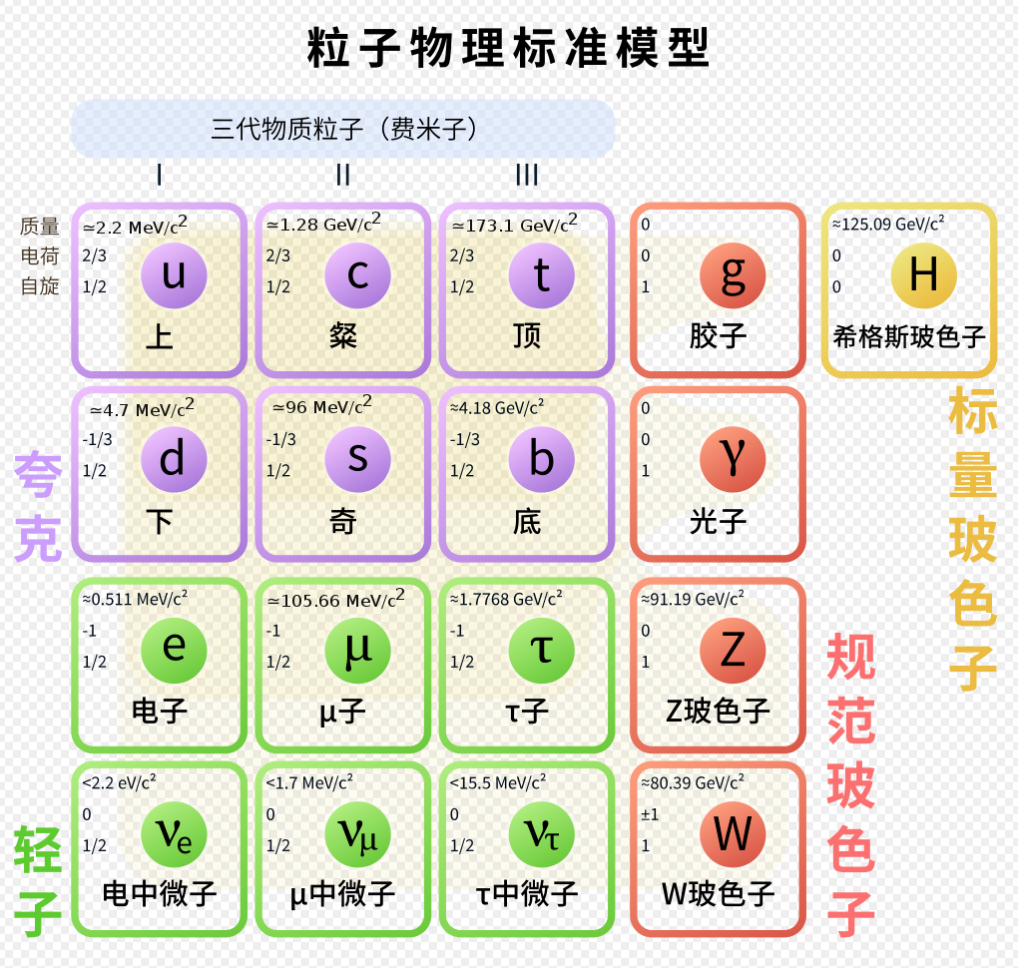
\includegraphics[width=0.50\textwidth]{figures/chapter01/SM.jpg}
    \bicaption{\quad \centering 粒子物理标准模型示意图~\cite{particlephys}}{\quad \centering Schematic diagram of Standard Model of particle physics~\cite{particlephys}}
    \label{fig:c01f01}
\end{figure}

其中,电荷用以描述微观粒子的带电荷量,根据不同微观粒子的带电性质,可以分为带正电荷的粒子、带负电荷的粒子以及不带电的中性粒子。在标准模型中,夸克、轻子和W玻色子带有电荷,剩下的中微子、胶子、光子以及希格斯粒子不带电,任何带电粒子都有与之对应的带相反电荷的反粒子。

自旋用以描述基本粒子的转动角动量这一性质,它的值是量子化的并且无法被改变。按照基本粒子的自旋特性,可以将基本粒子分为自旋为整数的玻色子和自旋为半整数的费米子。玻色子遵从玻色-爱因斯坦统计,对于全同的玻色子,波函数具有对称性,交换其中的两个粒子并不会改变波函数,这类粒子可以具有相同的量子态;而费米子遵从费米-狄拉克统计,对于全同的费米子,波函数具有反对称性,交换其中的两个粒子会使得波函数增加一个负号,这类粒子遵守泡利不相容原理,两个全同的费米子不能占据同样的量子态。在标准模型中,规范玻色子和希格斯粒子属于玻色子,夸克和轻子属于费米子。

色荷是夸克和胶子的一种内禀属性,用于描述处于不同状态的夸克和胶子。对于夸克来说,每种夸克有三种颜色:红色、绿色和蓝色,夸克的色荷可以处于这三种颜色之间;而胶子的色荷是由两种颜色混合而成,在量子色动力学中一共存在8种胶子。由于在量子色动力学中“色禁闭”效应的存在,由多个正反夸克构成的强子具有色中性的性质;而胶子的渐进自由特性使得它能够作为传递强相互作用的基本粒子。

基本粒子之间的相互作用可以根据相互作用的强度分为弱相互作用、电磁相互作用以及强相互作用,传递相互作用的媒介粒子分别为W、Z玻色子、光子以及胶子,对这些相互作用的描述可以通过规范场论来实现。

\subsection{电弱统一理论}

对于弱相互作用和电磁相互作用,电弱统一理论对其进行了成功地解释。电弱对称性发生自发破缺后的拉氏量可以表示为下面的形式:
\begin{equation}\label{eq:1-1}
    \mathcal{L}_{\mathrm{EW}}=\mathcal{L}_{\mathrm{K}}+\mathcal{L}_{\mathrm{N}}+\mathcal{L}_{\mathrm{C}}+\mathcal{L}_{\mathrm{H}}+\mathcal{L}_{\mathrm{HV}}+\mathcal{L}_{\mathrm{WWV}}+\mathcal{L}_{\mathrm{WWVV}}+\mathcal{L}_{\mathrm{Y}}
\end{equation}

动力学项$\mathcal{L}_{\mathrm{K}}$给出了拉氏量中的所有二次项(方程~\eqref{eq:1-2}),其中包含了费米子、规范玻色子、希格斯粒子的动力学项和质量项,$A_{\mu\nu}$、$Z_{\mu,\nu}$、$W^{\pm}_{\mu\nu}$分别表示对应的规范场,$f$表示费米子场,$H$表示希格斯场;中性流$\mathcal{L}_{\mathrm{N}}$(方程~\eqref{eq:1-3})和带电流$\mathcal{L}_{\mathrm{C}}$(方程~\eqref{eq:1-4})部分包含了费米子和规范玻色子之间的相互作用,其中CKM矩阵$M_{i j}^{\mathrm{CKM}}$确定了夸克的质量本征态和弱相互作用本征态之间的混合角度,$J_{\mu}^{em}$表示电磁流,$J_{\mu}^{3}$表示中性弱流;$\mathcal{L}_{\mathrm{H}}$描述了希格斯粒子的三顶点、四顶点自耦合相互作用项(方程~\eqref{eq:1-5});$\mathcal{L}_{\mathrm{HV}}$描述了希格斯粒子和规范矢量玻色子之间的相互作用(方程~\eqref{eq:1-6});$\mathcal{L}_{\mathrm{WWV}}$(方程~\eqref{eq:1-7})和$\mathcal{L}_{\mathrm{WWVV}}$(方程~\eqref{eq:1-8})描述了规范玻色子的三顶点、四顶点自耦合相互作用;$\mathcal{L}_{\mathrm{Y}}$描述了费米子和希格斯场之间的Yukawa相互作用(方程~\eqref{eq:1-9})。
\begin{equation}\label{eq:1-2}
    \begin{array}{r}
        \mathcal{L}_{\mathrm{K}}=\sum_{f} \bar{f}(i \not\partial -m_{f}) f-\frac{1}{4} A_{\mu \nu} A^{\mu \nu}-\frac{1}{2} W_{\mu \nu}^{+} W^{-\mu \nu}+m_{W}^{2} W_{\mu}^{+} W^{-\mu} \\
        -\frac{1}{4} Z_{\mu \nu} Z^{\mu \nu}+\frac{1}{2} m_{Z}^{2} Z_{\mu} Z^{\mu}+\frac{1}{2}(\partial^{\mu} H)(\partial_{\mu} H)-\frac{1}{2} m_{H}^{2} H^{2}
    \end{array}
\end{equation}

\begin{equation}\label{eq:1-3}
    \mathcal{L}_{\mathrm{N}}=e J_{\mu}^{\mathrm{em}} A^{\mu}+\frac{g}{\cos \theta_{W}}\left(J_{\mu}^{3}-\sin ^{2} \theta_{W} J_{\mu}^{\mathrm{em}}\right) Z^{\mu}
\end{equation}

\begin{equation}\label{eq:1-4}
    \mathcal{L}_{\mathrm{C}}=-\frac{g}{\sqrt{2}}\left[\bar{u}_{i} \gamma^{\mu} \frac{1-\gamma^{5}}{2} M_{i j}^{\mathrm{CKM}} d_{j}+\bar{\nu}_{i} \gamma^{\mu} \frac{1-\gamma^{5}}{2} e_{i}\right] W_{\mu}^{+}+\text {h.c. }
\end{equation}

\begin{equation}\label{eq:1-5}
    \mathcal{L}_{\mathrm{H}}=-\frac{g m_{\mathrm{H}}^{2}}{4 m_{\mathrm{W}}} H^{3}-\frac{g^{2} m_{\mathrm{H}}^{2}}{32 m_{\mathrm{W}}^{2}} H^{4}
\end{equation}

\begin{equation}\label{eq:1-6}
    \mathcal{L}_{\mathrm{HV}}=\left(g m_{\mathrm{HV}}+\frac{g^{2}}{4} H^{2}\right)\left(W_{\mu}^{+} W^{-\mu}+\frac{1}{2 \cos ^{2} \theta_{\mathrm{W}}} Z_{\mu} Z^{\mu}\right)
\end{equation}

\begin{equation}\label{eq:1-7}
    \begin{aligned}
        \mathcal{L}_{\mathrm{WWV}} & =-i g[\left(W_{\mu \nu}^{+} W^{-\mu}-W^{+\mu} W_{\mu \nu}^{-}\right)\left(A^{\nu} \sin \theta_{\mathrm{W}}-Z^{\nu} \cos \theta_{\mathrm{W}}\right) \\
        &+W_{\nu}^{-} W_{\mu}^{+}\left(A^{\mu \nu} \sin \theta_{\mathrm{W}}-Z^{\mu \nu} \cos \theta_{\mathrm{W}}\right)]
    \end{aligned}
\end{equation}

\begin{equation}\label{eq:1-8}
    \begin{aligned}
    & \mathcal{L}_{\mathrm{WWVV}} =-\frac{g^{2}}{4}\{ {\left[2 W_{\mu}^{+} W^{-\mu}+\left(A_{\mu} \sin \theta_{\mathrm{W}}-Z_{\mu} \cos \theta_{\mathrm{W}}\right)^{2}\right]^{2} } \\
    & \left.-\left[W_{\mu}^{+} W_{\nu}^{-}+W_{\nu}^{+} W_{\mu}^{-}+\left(A_{\mu} \sin \theta_{\mathrm{W}}-Z_{\mu} \cos \theta_{\mathrm{W}}\right)(A_{\nu} \sin \theta_{\mathrm{W}}-Z_{\nu} \cos \theta_{\mathrm{W}}\right)\right]^{2} \}
\end{aligned}
\end{equation}

\begin{equation}\label{eq:1-9}
    \mathcal{L}_{\mathrm{Y}}=-\sum_{f} \frac{g m_{f}}{2 m_{\mathrm{W}}} \bar{f} f H
\end{equation}

\subsection{量子色动力学}

对于夸克和胶子之间的强相互作用力,量子色动力学对其进行了阐述。规范不变的量子色动力学拉氏量可以写为如下形式:
\begin{equation}\label{eq:1-10}
    \mathcal{L}_{\mathrm{QCD}}=\bar{\psi}_{i}\left(i \gamma^{\mu}\left(D_{\mu}\right)_{i j}-m \delta_{i j}\right) \psi_{j}-\frac{1}{4} G_{\mu \nu}^{a} G_{a}^{\mu \nu}
\end{equation}

其中,$\psi_{i}(x)$是夸克场,它是时空的函数;$G_{\mu \nu}^{a}$表示规范不变的胶子场强张量,具体表达式为(方程~\eqref{eq:1-11}),$\mathcal{A}_{\mu}^{a}(x)$表示胶子场;变量$m$和$g$分别对应于夸克的质量和耦合顶点参数。
\begin{equation}\label{eq:1-11}
    G_{\mu \nu}^{a}=\partial_{\mu} \mathcal{A}_{\nu}^{a}-\partial_{\nu} \mathcal{A}_{\mu}^{a}+g f^{a b c} \mathcal{A}_{\mu}^{b} \mathcal{A}_{\nu}^{c}
\end{equation}

\subsection{超出标准模型的新物理}

标准模型可以解释目前粒子物理实验上观测到的绝大多数的物理现象。然而,标准模型并不是一个完美地理论,仍然存在许多标准模型无法解释的物理现象,比如说:暗物质、暗能量、中微子质量、正反物质不对称等等。这就意味着我们仍然需要寻找超出标准模型的新物理。

根据当前宇宙学标准模型的计算,宇宙中大约 27\% 是暗物质;68\% 是暗能
量。构成恒星、行星和生物的介子只占宇宙总质量的大约 5\%。这也就是说,标准模型只能解释宇宙中的极少部分组成。到目前为止,人们认为暗物质的可能的存在形式是粒子形式,对应的可能粒子主要有以下几种:
\begin{itemize}
    \item 低质量玻色子:包括量子色动力学轴子~\cite{Bandyopadhyay_2019}、类轴子和模糊冷暗物质~\cite{PhysRevLett.85.1158}等;
    \item 中微子:包括标准模型中微子和惰性中微子~\cite{Boyarsky_2019};
    \item 弱尺度下的新粒子:比如超对称~\cite{1966PThPh..36.1266M}、额外维度~\cite{rizzo2004pedagogical}、有效场论~\cite{Criado_2021}等等;
    \item 其他粒子:比如大质量弱相互作用粒子~\cite{Jungman_1996}(Weakly Interacting Massive Particles,WIMPs)、自相互作用的暗物质~\cite{PhysRevLett.84.3760}等等。
\end{itemize}

在标准模型中,希格斯玻色子作为唯一的标量粒子,赋予了所有基本粒子以质量,这就使得暗物质粒子的质量起源可能和希格斯粒子有关。因此,寻找希格斯粒子与暗物质粒子的相互作用是一个前沿热点课题。近年来,LHC上的ATLAS实验和CMS实验都对以上可能的暗物质粒子进行了寻找,对许多新物理模型给出了排除限制。当然,其中也不乏利用希格斯粒子来对暗物质进行寻找。其中,对希格斯粒子衰变到不可探测粒子的测量就是一个很好的例子。在标准模型中,由于中微子不具有质量并且几乎不与任何物质发生相互作用,使得中微子成为了在对撞机中唯一不能够被探测到的粒子。根据标准模型的计算,希格斯粒子衰变到中微子的分支比仅占0.1\%~\cite{Dittmaier:2011ti}。而根据CMS实验的最新测量结果,希格斯粒子衰变到不可探测粒子的分支比排除上限仅为18\%~\cite{Hinv}。这就意味着它们中间可能会包含有无法被探测器捕捉到的超出标准模型的新粒子的存在,比如长寿命的暗物质粒子,使得测量结果远超出标准模型的计算。因此,寻找这类超出标准模型的新物理具有非常重要的物理意义。

\section{类轴子}
\label{sec:first}
类轴子(Axion-Like Particles, ALPs)模型描述了一种全新的基本粒子,这种粒子是一个规范单态的赝标量粒子,并且具有近似的平移对称性这一特性,因此它的质量通常会比电弱标度甚至QCD标度更小。对于类轴子的描述可以通过有效场论来完成~\cite{PhysRevLett.119.031802,Bauer:2017ris},最简单的维度小于5的有效拉氏量可以写为:
\begin{equation}\label{eq:1-12}
    \begin{aligned}
    \mathcal{L}_{\text {eff }}^{D \leq 5}= & \frac{1}{2}(\partial_{\mu} a)\left(\partial^{\mu} a\right)-\frac{m_{a, 0}^{2}}{2} a^{2}+\frac{\partial^{\mu} a}{\Lambda} \sum_{F} \bar{\psi}_{F} \boldsymbol{C}_{F} \gamma_{\mu} \psi_{F} \\
    & +g_{s}^{2} C_{G G} \frac{a}{\Lambda} G_{\mu \nu}^{A} \tilde{G}^{\mu \nu, A}+g^{2} C_{W W} \frac{a}{\Lambda} W_{\mu \nu}^{A} \tilde{W}^{\mu \nu, A}+g^{\prime 2} C_{B B} \frac{a}{\Lambda} B_{\mu \nu} \tilde{B}^{\mu \nu},
    \end{aligned}
\end{equation}
其中包含了不满足平移对称性的质量项$m_{a, 0}^{2}$;$G_{\mu \nu}^{A}$、$W_{\mu \nu}^{A}$和$B_{\mu \nu}$分别表示了$SU(3)_c$、$SU(2)_L$和$U(1)_Y$场强张量,$g_s$、$g$和$g'$分别表示了对应的耦合常数;$\Lambda$表示新物理的标度,这是全局对称性破缺的特征尺度。

然而在树图水平上,五阶算符不存在$H\rightarrow Z\gamma$的耦合顶点,这一衰变道被圈图效应所压低,使得在探测器上对这一衰变道的寻找变得极为困难。但是,我们可以通过构建更高阶的算符来产生树图阶的贡献。六维以上的有效拉氏量可以写为:
\begin{equation}\label{eq:1-13}
    \mathcal{L}_{\mathrm{eff}}^{D \geq 6}=\frac{C_{a h}}{\Lambda^{2}}(\partial_{\mu} a)\left(\partial^{\mu} a\right) \phi^{\dagger} \phi+\frac{C_{a h}^{\prime}}{\Lambda^{2}} m_{a, 0}^{2} a^{2} \phi^{\dagger} \phi+\frac{C_{Z h}^{(7)}}{\Lambda^{3}}\left(\partial^{\mu} a\right)\left(\phi^{\dagger} i D_{\mu} \phi+\text { h.c. }\right) \phi^{\dagger} \phi+\ldots 
\end{equation}
其中前两项给出了对$H\rightarrow aa$衰变道的贡献;第三项给出了领头阶的$H\rightarrow Z\gamma$树图衰变贡献。在经过电弱对称性破缺后,有效拉氏量~\eqref{eq:1-12}给出了类轴子和$\gamma\gamma$、$\gamma Z$以及$ZZ$之间的耦合参数,对应的表达式可以写为:

\begin{equation}\label{eq:1-14}
    \mathcal{L}_{\text {eff }}^{D \leq 5} \ni e^{2} C_{\gamma \gamma} \frac{a}{\Lambda} F_{\mu \nu} \tilde{F}^{\mu \nu}+\frac{2 e^{2}}{s_{w} c_{w}} C_{\gamma Z} \frac{a}{\Lambda} F_{\mu \nu} \tilde{Z}^{\mu \nu}+\frac{e^{2}}{s_{w}^{2} c_{w}^{2}} C_{Z Z} \frac{a}{\Lambda} Z_{\mu \nu} \tilde{Z}^{\mu \nu}
\end{equation}

至此,类轴子模型的有效拉氏量基本构建完成。拉氏量~\eqref{eq:1-12}给出了类轴子衰变到一对标准模型规范玻色子和费米子的耦合参数,比如:$a\rightarrow \gamma\gamma$、$a\rightarrow \ell\ell$、$a\rightarrow q\bar{q}$和$a\rightarrow gg$。对于类轴子的产生模式,拉氏量~\eqref{eq:1-13}和~\eqref{eq:1-14}分别给出了$H\rightarrow aa$和$H\rightarrow Za$的一阶圈图修正和领头阶树图的贡献。

\subsection{缪子反常磁矩}

自旋磁矩作为基本粒子的内禀属性之一,通常表述为g因子,可以通过实验或者理论计算得到。根据狄拉克方程预言,电子或者缪子的g因子为2,这对应于量子电动力学中的树图解释。然而,高阶圈图修正会对g因子的计算产生影响。此时,我们将实验观测结果和树图结果的差值百分比定义为反常磁矩$a$:
\begin{equation}\label{eq:1-15}
    a = \frac{g-2}{2}
\end{equation}
反常磁矩的测量结果和理论计算结果对精确检验量子电动力学的正确性具有非常重要的意义。目前,根据Muon g-2合作组的最新测量,缪子反常磁矩的测量结果为$a=0.00116592061(41)$\cite{abi2021measurement}。然而,在考虑了电弱修正和强子修正之后,理论计算和实验结果之间的偏差仍然达到了4.2个标准偏差,这就意味着其间很有可能存在超出标准模型的新物理。

\begin{figure}[!htbp]
    \centering
    %trim option's parameter order: left bottom right top
    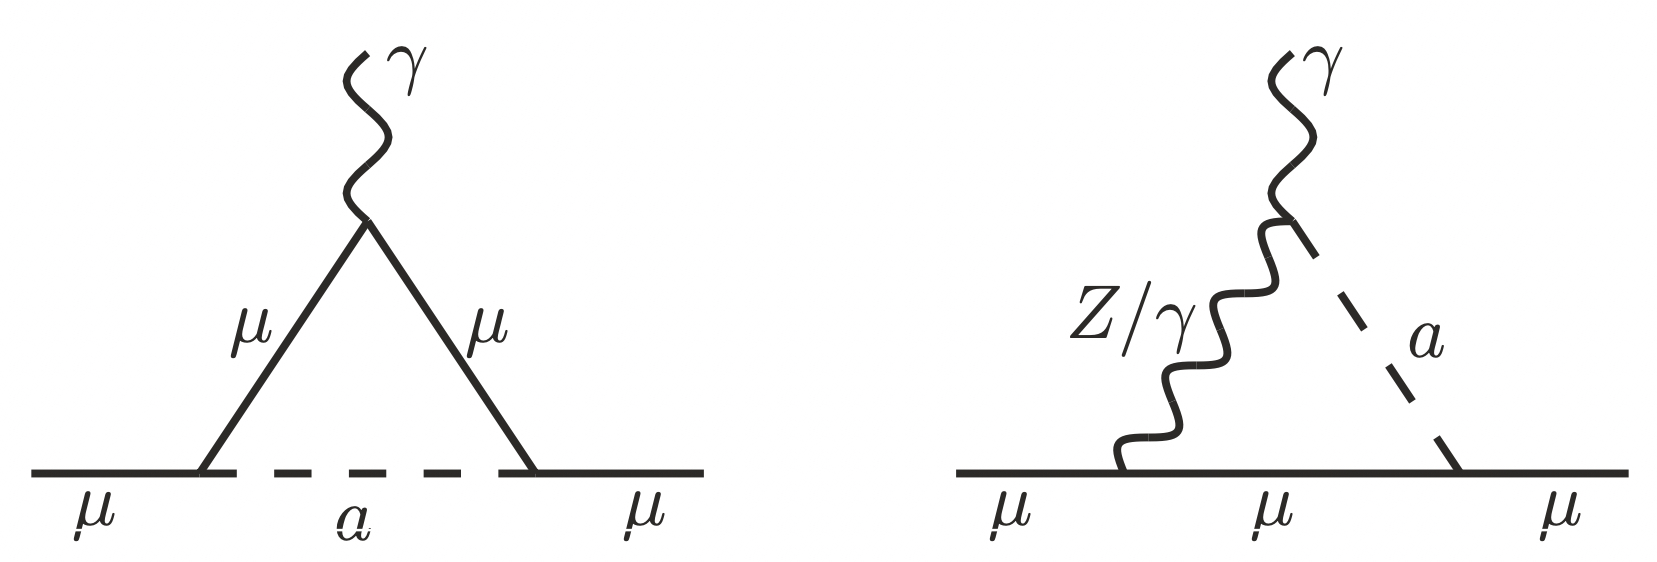
\includegraphics[width=0.60\textwidth]{figures/chapter01/ALP_g_2.jpg}
    \bicaption{\quad \centering 类轴子模型单圈费曼图对缪子反常磁矩的贡献~\cite{Bauer:2017ris}}{\quad \centering One-loop Feyman diagrams contributing to the anomalous magnetic moment of the muon for Axion-Like Particles Model~\cite{Bauer:2017ris}}
    \label{fig:c01f02}
\end{figure}

类轴子模型可以为缪子反常磁矩的偏差提供理论解释。在单圈图阶段,类轴子模型有效拉氏量对缪子反常磁矩的贡献可以通过费曼图\ref{fig:c01f02}进行描述。通过计算,类轴子模型引起的新物理贡献可以表示为:
\begin{equation}\label{eq:1-16}
    \begin{array}{c}
    \delta a_{\mu}=\frac{m_{\mu}^{2}}{\Lambda^{2}}\left\{K_{a_{\mu}}(\mu)-\frac{\left(c_{\mu \mu}\right)^{2}}{16 \pi^{2}} h_{1}\left(\frac{m_{a}^{2}}{m_{\mu}^{2}}\right)-\frac{2 \alpha}{\pi} c_{\mu \mu} C_{\gamma \gamma}\left[\ln \frac{\mu^{2}}{m_{\mu}^{2}}+\delta_{2}+3-h_{2}\left(\frac{m_{a}^{2}}{m_{\mu}^{2}}\right)\right]\right. \\
    \left.-\frac{\alpha}{2 \pi} \frac{1-4 s_{w}^{2}}{s_{w} c_{w}} c_{\mu \mu} C_{\gamma Z}\left(\ln \frac{\mu^{2}}{m_{Z}^{2}}+\delta_{2}+\frac{3}{2}\right)\right\} 
    \end{array}
\end{equation}
其中,
\begin{equation}\label{eq:1-17}
    \begin{array}{l}
    h_{1}(x)=1+2 x+x(1-x) \ln x-2 x(3-x) \sqrt{\frac{x}{4-x}} \arccos \frac{\sqrt{x}}{2} \\
    h_{2}(x)=1-\frac{x}{3}+\frac{x^{2}}{6} \ln x+\frac{2+x}{3} \sqrt{x(4-x)} \arccos \frac{\sqrt{x}}{2}
    \end{array}
\end{equation}

图\ref{fig:c01f03}展示了可以用来解释实验上所观测到的缪子反常磁矩的类轴子模型的参数空间。其中,红色、橘色和黄色范围分别表示可以在68\%、95\%和99\%的置信度上解释实验上观测到的缪子反常磁矩的类轴子模型的参数空间范围;灰色区域表示可以被BaBar实验中对暗光子的寻找所排除的参数空间范围。目前为止,仍然没有实验结果可以完全排除类轴子模型对缪子反常磁矩的贡献。因此,类轴子的寻找对了解缪子反常磁矩具有非常重要的物理意义。

\begin{figure}[!htbp]
    \centering
    %trim option's parameter order: left bottom right top
    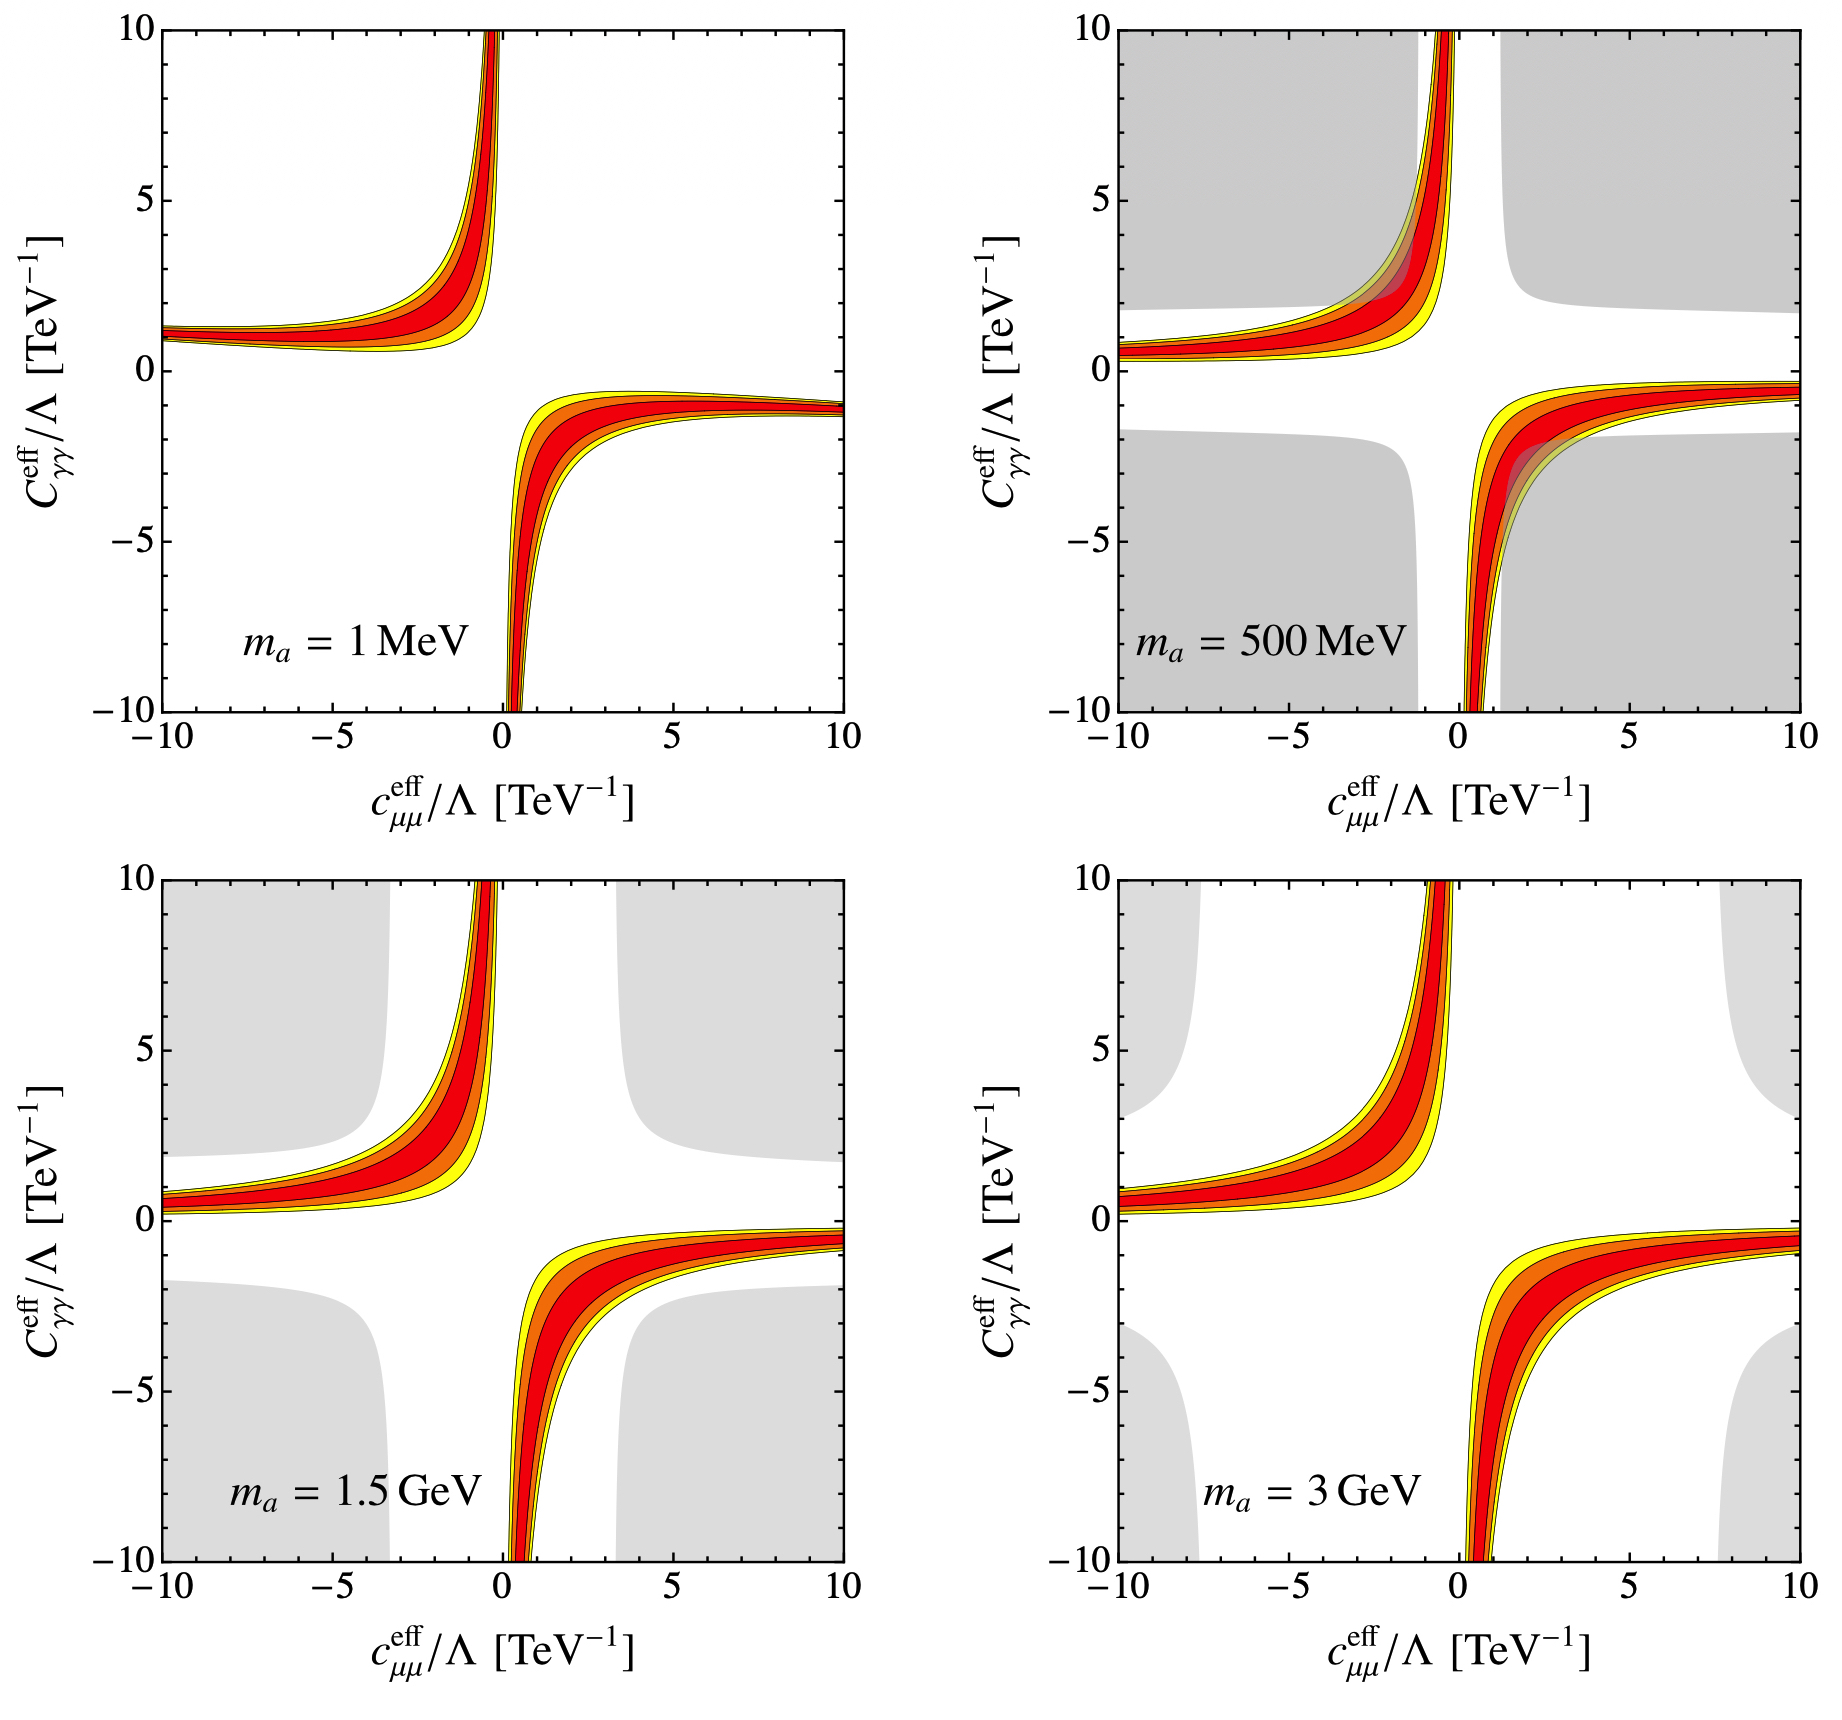
\includegraphics[width=0.85\textwidth]{figures/chapter01/ALP_cuu.jpg}
    \bicaption{\quad \centering 对于不同质量的类轴子,可以在68\%(红色), 95\% (橙色)和99\%(黄色)的置信度上重现$(g-2)_\mu$试验结果的类轴子耦合参数空间。灰色区域表示可以被BaBar实验中对暗光子的寻找所排除的参数空间范围~\cite{Bauer:2017ris}}{\quad \centering Regions in ALP coupling space where the experimental value of $(g-2)_\mu$ is reproduced at 68\% (red), 95\% (orange) and 99\% (yellow) confidence level (CL), for different values of $m_a$. The gray regions are excluded by a dark-photon search performed by BaBar~\cite{Bauer:2017ris}}
    \centering
    \label{fig:c01f03}
\end{figure}

\subsection{冷暗物质候选者}

当类轴子的质量非常小或者与标准模型的相互作用非常弱的时候,类轴子会具有非常长的寿命,这就使得类轴子在衰变到可以被探测器接收到的末态粒子之前就已经飞出了探测器,在探测器中表现为丢失的能量。在这种情况下,类轴子可以作为冷暗物质的候选体~\cite{PhysRevLett.119.031802}。

\subsection{现有研究成果}

图~\ref{fig:c01f04}展示了不同实验对类轴子和光子之间的耦合强度以及类轴子质量的限制范围,横坐标为类轴子的质量,纵坐标为类轴子和光子的耦合强度。其中,红色区域表示可以通过类轴子模型解释实验上观测到的缪子反常磁矩的参数空间范围;淡绿色区域表示在LHC上利用全部二期运行数据对$H\rightarrow Za$衰变道的寻找预计可以排除的类轴子参数空间范围,点线、虚线和实线分别对应于不同的$H\rightarrow Za$耦合强度。因此,大型强子对撞机对类轴子的寻找具有非常高的灵敏度,它可以探测到其他实验所无法探测到的参数空间。此外,通过对$H\rightarrow Za$衰变道的寻找可以让我们对缪子反常磁矩具有更深刻的认识。

\begin{figure}[!htbp]
    \centering
    %trim option's parameter order: left bottom right top
    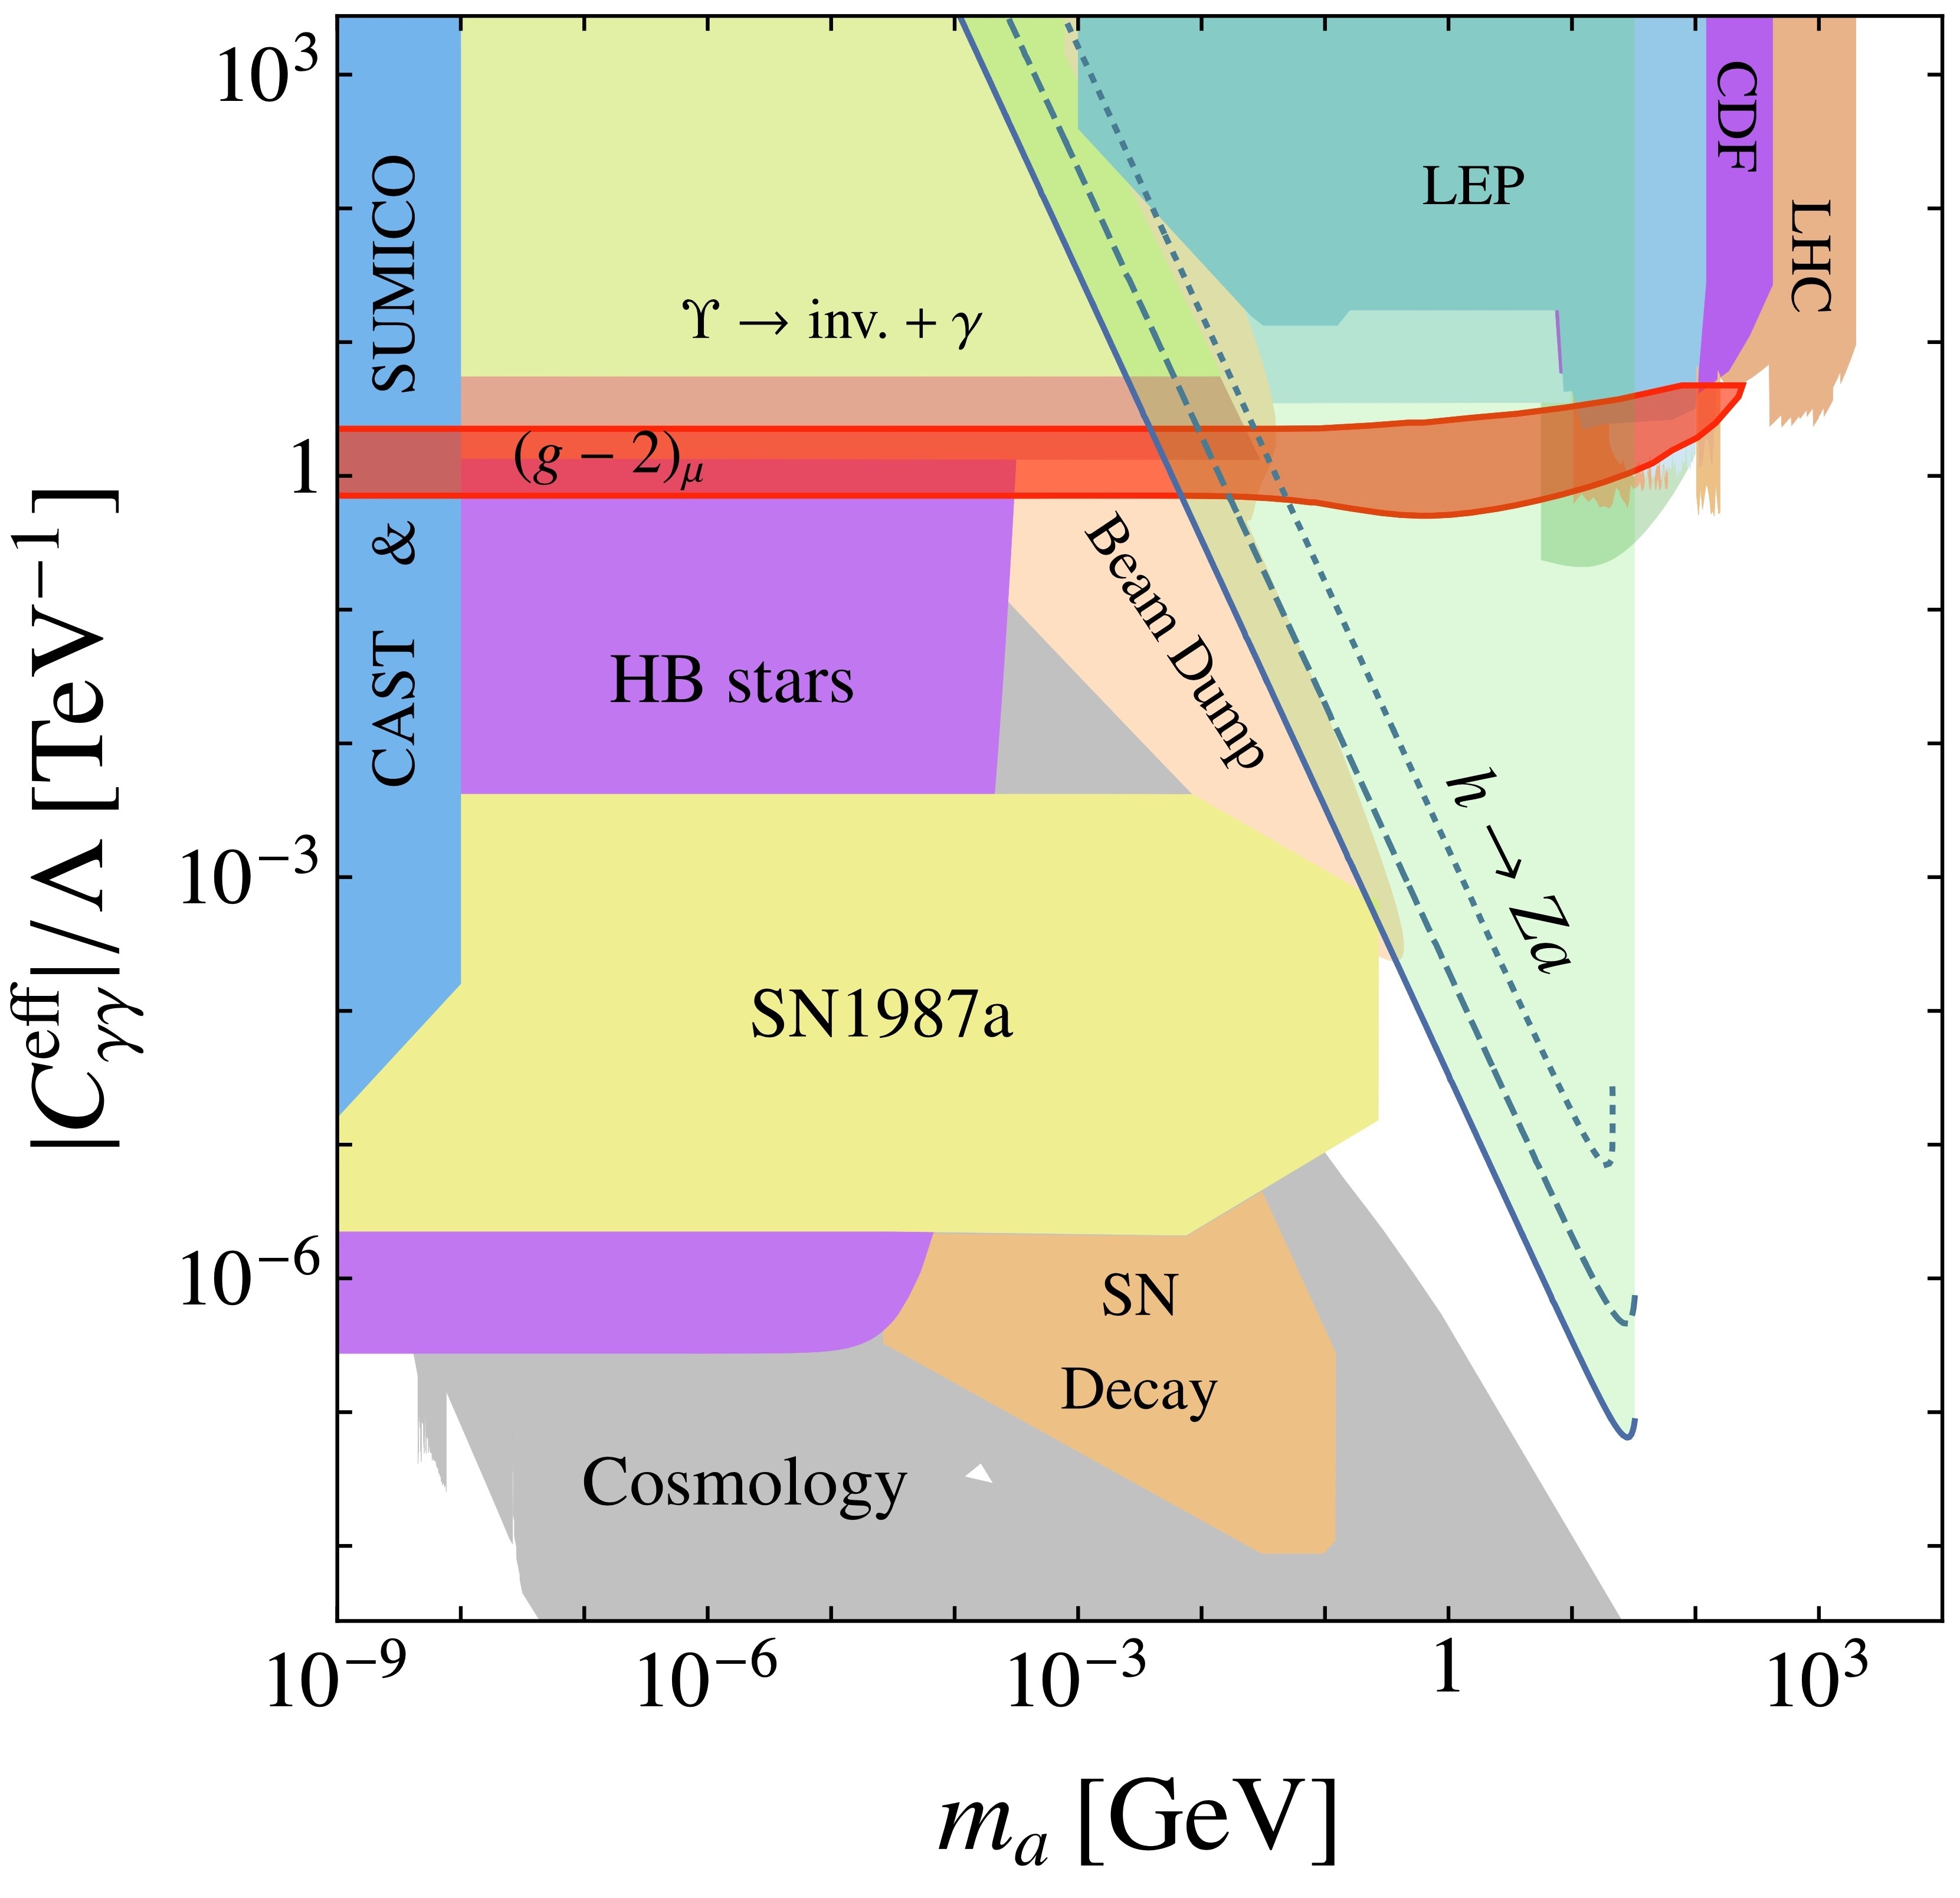
\includegraphics[width=0.70\textwidth]{figures/chapter01/ALP_run2.jpg}
    \bicaption{\quad \centering 不同实验对类轴子质量和与光子之间耦合强度的限制以及可以通过LHC上的$\HZa$衰变道探测的参数空间范围。绿色的点线、虚线和实线轮廓分别对应于$\cZh = 0.72~\si{\TeV^{-1}}$、$0.1~\si{\TeV^{-1}}$、和$0.015~\si{\TeV^{-1}}$。红色区域显示了可以在95\%置信度水平上解释缪子反常磁矩的参数空间~\cite{Bauer:2017ris}}{\quad \centering Constraints on the ALP mass and coupling to photons derived from various experiments along with the parameter regions that can be probed using the Higgs decays $\HZa$ on LHC. The green contours correspond to $\cZh = 0.72~\si{\TeV^{-1}}$ (solid), $0.1~\si{\TeV^{-1}}$ (dashed) and $0.015~\si{\TeV^{-1}}$
    (dotted). The red band shows the preferred parameter space where the $(g-2)_\mu$ anomaly can be explained at 95\% CL~\cite{Bauer:2017ris}}
    \label{fig:c01f04}
\end{figure}

到目前为止,CMS实验和ATLAS实验对不同产生模式和衰变模式下的类轴子进行了寻找。比如:利用Pb--Pb对撞的光子光子散射来寻找类轴子~\cite{aad2021measurement,sirunyan2019evidence};通过研究两个光子在探测器中融合为一个光子喷注来寻找类轴子~\cite{cms2022search,atlas2022search};通过希格斯粒子衰变到四个光子末态来寻找类轴子~\cite{CMS_ALP_1};通过希格斯粒子衰变到四个轻子末态来寻找类轴子~\cite{CMS_ALP_3}。

但是,目前还没有实验对$\HZa$进行过测量。本分析给出了LHC上对希格斯粒子衰变到双轻子加双光子末态的首次测量结果,并且也给出了对类轴子耦合强度的测量结果。

\section{利用希格斯粒子衰变到两轻子加两光子末态来寻找类轴子}

希格斯粒子衰变到一个Z玻色子和一个类轴子的费曼图可以表示为图~\ref{fig:c01f05},其中只考虑了树图水平和单圈图水平。前两项的圈图贡献来自于五维有效拉氏量,最后一项的树图贡献来自于更高阶的有效拉氏量。

\begin{figure}[!htbp]
    \centering
    %trim option's parameter order: left bottom right top
    
\includegraphics[width=0.9\textwidth]{figures/chapter01/ALP_feynman.jpg}
    \bicaption{\quad \centering 对$H\rightarrow Za$有贡献的费曼图~\cite{Bauer:2017ris}}{\quad \centering Feynman diagrams contributing to the decay $H\rightarrow Za$~\cite{Bauer:2017ris}}
    \label{fig:c01f05}
\end{figure}

考虑了所有贡献以后,$H\rightarrow Za$的宽度表达式为
\begin{equation}\label{eq:1-18}
    \Gamma(h \rightarrow Z a)=\frac{m_{h}^{3}}{16 \pi \Lambda^{2}}\left|\frac{C_{\mathrm{Zh}}^{\mathrm{eff}}}{\Lambda}\right|^{2} \lambda^{3 / 2}\left(\frac{m_{Z}^{2}}{m_{h}^{2}}, \frac{m_{a}^{2}}{m_{h}^{2}}\right)
\end{equation}
其中,$\lambda(x,y) = (1-x-y)^2 -4xy$。

在本分析中,Z玻色子最终衰变为两个味道相同、带相反电荷的轻子(电子或缪子);类轴子最终衰变为两个光子,对应的衰变宽度可以表示为
\begin{equation}\label{eq:1-19}
    \Gamma(a \rightarrow \gamma \gamma) \equiv \frac{4 \pi \alpha^{2} m_{a}^{3}}{\Lambda^{2}}\left|C_{\gamma \gamma}^{\mathrm{eff}}\right|^{2}
\end{equation}
对于质量小于两个电子质量的低质量类轴子,标准模型衰变模式中唯一允许的衰变末态是双光子末态。此时,类轴子衰变到双光子会具有非常长的寿命,而且质量越小寿命越长。最终,类轴子会在衰变为可以被探测器捕捉到的两个光子末态之前就飞出探测器,表现为丢失的能量。在此分析中,我们仅关注希格斯粒子的奇异衰变,因此类轴子衰变到双光子末态的分支比被设定为100\%。

根据$H\rightarrow Za$的动力学性质,由于我们要求一个在壳的Z玻色子,由希格斯粒子衰变而来的低质量类轴子会具有非常高的横动量,使得类轴子衰变产生的两个光子具有非常小的角距离,最终在探测器里会表现为一个融合的光子喷注。此时,$H\rightarrow Za$会对$H\rightarrow Z\gamma$的宽度测量产生贡献,使得$H\rightarrow Z\gamma$的宽度测量相对于标准模型的预言偏大。图~\ref{fig:c01f06}展示了$h \rightarrow Z a$的宽度和标准模型$h \rightarrow Z \gamma$宽度的比值作为有效威尔逊系数$\cZh$的函数,在一定参数空间,类轴子可以对标准模型$h \rightarrow Z \gamma$的寻找产生很大的影响。

\begin{figure}[!htbp]
    \centering
    %trim option's parameter order: left bottom right top
    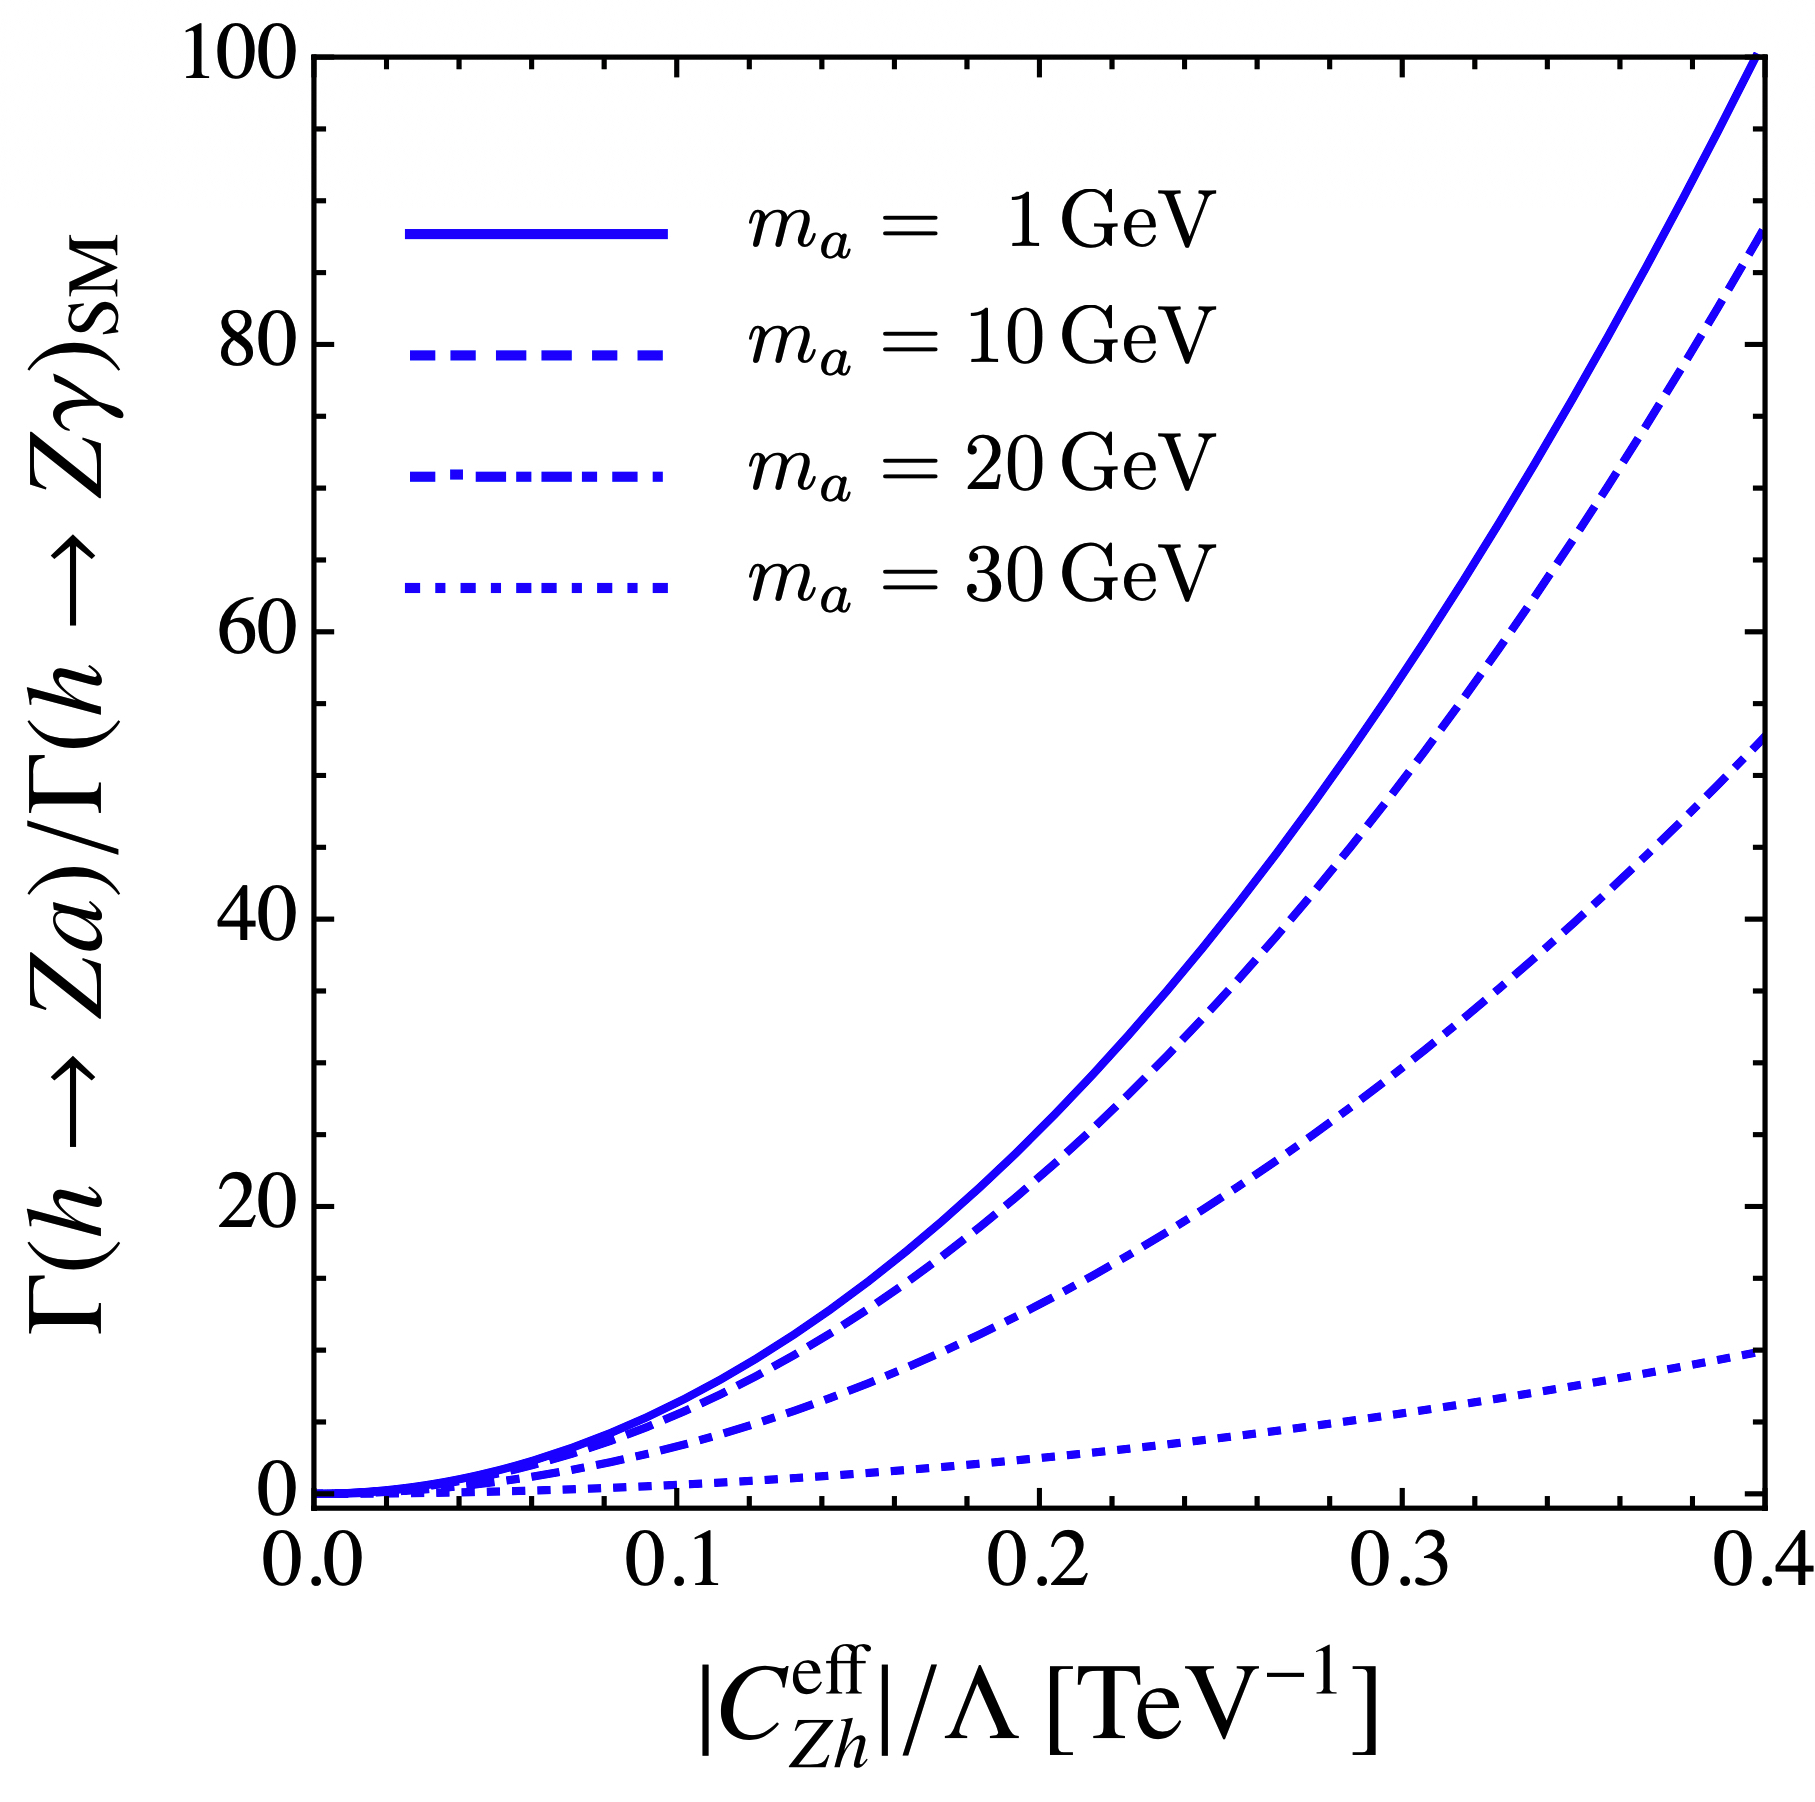
\includegraphics[width=0.5\textwidth]{figures/chapter01/ALP_GammaRatio.jpg}
    \bicaption{\quad \centering 对于不同的类轴子质量,比值$\Gamma(h \rightarrow Z a) / \Gamma(h \rightarrow Z \gamma)_{\mathrm{SM}}$作为有效威尔逊系数$\cZh$的函数~\cite{Bauer:2017ris}}{\quad \centering The ratio of $\Gamma(h \rightarrow Z a) / \Gamma(h \rightarrow Z \gamma)_{\mathrm{SM}}$ as a function of the effective Wilson coefficient $\cZh$ for different ALP masses~\cite{Bauer:2017ris}}
    \label{fig:c01f06}
\end{figure}

\subsection{研究的物理意义}

首先,此研究可以作为与模型无关的低质量双光子共振态的寻找。到目前为止,LHC上尚未有希格斯粒子衰变到双光子加双轻子末态的测量结果,此分析给出了希格斯粒子在双轻子加双光子末态下的首次测量结果,并对质量范围为1--30$\GeV$之间的低质量双光子共振态进行了寻找,让我们对希格斯粒子的奇异衰变有了更深刻的理解。

其次,此分析首次利用了$\HZa$衰变道对类轴子进行了寻找。根据图~\ref{fig:c01f04}所示,在LHC上通过$\HZa$衰变道对类轴子的寻找具有非常高的灵敏度,测量结果可以覆盖到其他实验所不能探测的参数空间。此外,在一定的参数空间范围中,类轴子模型可以解释实验上观测到的缪子反常磁矩的物理现象,对类轴子的寻找可以让我们对缪子反常磁矩具有更深刻的理解。

\subsection{研究难点}

首先,本分析所要求的信号事例末态两个光子的横动量比较低。由于要求Higgs衰变产生一个在壳的Z玻色子和类轴子,根据衰变的动力学分析,类轴子的质量大概在小于30$\GeV$的范围内。因此,信号事例末态两个光子的横动量大部分集中在10$\GeV$到15$\GeV$之间。而在CMS实验中,默认的光子辨别算法要求横动量大于15$\GeV$,这就使得传统默认的CMS光子辨别算法不再适用于本分析。

其次,在低质量类轴子区间(小于5$\GeV$),信号事例末态两个光子的角距离非常小。由于类轴子的质量非常小,使得从希格斯粒子衰变产生的类轴子具有比较高的横动量,进而使得类轴子衰变产生的两个光子具有非常高的横动量,使得这两个光子具有非常小的角距离,无法在探测器中识别并重建出两个光子。

最后,本分析具有非常低的信噪比。由于在信号区间存在大量的假光子和与信号事例无关的标准模型过程等本底,使得最终的信号显著度非常低。

\subsection{研究方法}

本分析利用了CMS探测器整个二期运行期间(2016年、2017年和2018年)收集到的138~\si{fb^{-1}}的数据对$\HZa$进行了寻找,其中轻子部分仅包括电子和缪子。针对以上难点,本分析提供了以下解决办法。

首先,本分析研究了传统光子辨别算法中各个变量对信号事例的影响,设计了新的光子鉴别算法,使得信号效率在低质量区间获得了显著的提升。

为了进一步提高信号显著度,本分析采用了多变量分析的方法,利用光子和类轴子的动力学等信息作为输入对信号和本底进行区分,最终使得信号显著度获得了显著的提升。

%%% Local Variables: 
%%% mode: latex
%%% TeX-master: t
%%% End: 

\chapter{LHC和CMS探测器}

\section{LHC简介}

LHC(Large Hadron Collider,LHC)全称大型强子对撞机,是由欧洲核子研究中心(Conseil Européen pour la Recherche Nucléaire,CERN)建造的目前世界上最大的、能量最高的粒子对撞机。它坐落于瑞士日内瓦和法国边境(图~\ref{fig:c02f01}),周长26.7公里,隧道位于地下50米至170米,可以将两束质子束流加速到接近光速并发生对撞。2008年9月10号,LHC开始首次运行,并于2010年在3.5 TeV的质心能量下发生首次对撞。LHC主要由两部分组成:用于加速粒子束流和发生对撞的加速器部分;用于探测对撞粒子的探测器部分。

\begin{figure}[!htbp]
    \centering
    %trim option's parameter order: left bottom right top
    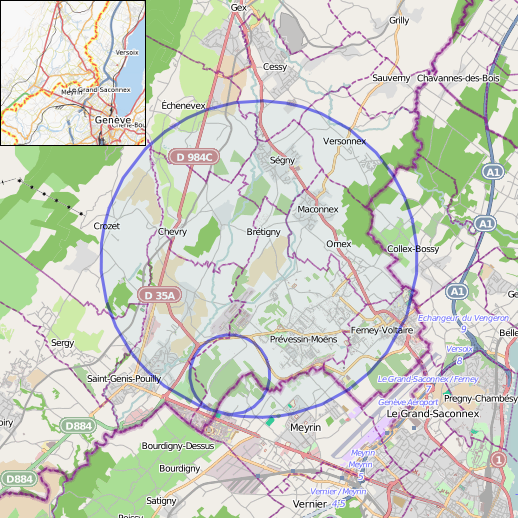
\includegraphics[width=0.5\textwidth]{figures/chapter02/Location_Large_Hadron_Collider.png}
    \bicaption{\quad \centering 大型强子对撞机(LHC)位置图~\cite{LHC}}{\quad \centering Map of the Large Hadron Collider~\cite{LHC}(LHC)}
    \label{fig:c02f01}
\end{figure}

加速器部分主要由27公里的超导磁铁环和许多加速结构构成,用于加速经过的粒子束流。在加速器内部,两束高能粒子束流可以被加速到接近光速,并且以相反的运动方向在由超导电磁体产生的强电磁场中沿着束流管道运行。超导电磁体包括了1232个偶极磁铁和392个四极磁铁。每个偶极磁铁长约15米,主要用于使粒子束流轨迹发生弯曲;每个四极磁铁长约5到7米,主要作用是聚焦束流。加速结构主要指的是射频腔,带电粒子在射频腔产生的强电场内被不断加速,通过多级加速结构,最终可以使得粒子束流的速度接近于光速的99.9999991\%。图~\ref{fig:c02f02}展示了粒子束流的加速过程:

\begin{enumerate}
    \item 通过将氢原子的核外电子剥离得到质子束流,并在直线加速器的作用下将质子束流加速到50~\si{\MeV}。
    \item 将加速后的质子束流注入到质子同步推进器中继续加速至1.4~\si{\GeV}。
    \item 继续将加速后的质子束流注入质子同步加速器中加速至25~\si{\GeV}。
    \item 质子束流被注入到超级质子同步加速器中,加速到450~\si{\GeV}。
    \item 最终,两束质子束流被分别注入到LHC的两个束流管中,以相反的方向运动,加速至7~\si{\TeV}。
\end{enumerate}

\begin{figure}[!htbp]
    \centering
    %trim option's parameter order: left bottom right top
    \includegraphics[width=1.0\textwidth]{figures/chapter02/CERN_accelerator.jpeg}
    \bicaption{\quad \centering CERN加速器综合体~\cite{accelerator}}{\quad \centering The CERN accelerator complex~\cite{accelerator}}
    \label{fig:c02f02}
\end{figure}

粒子探测器主要用于探测高能粒子发生对撞后所产生的末态粒子。根据这些产生的末态粒子,可以反推得到粒子对撞时发生的物理过程,这也是我们了解微观粒子世界的重要途径。在LHC建设之初,一共有9个探测器被建造出来,它们分别位于LHC的不同对撞点上,具有各自不同的物理实验目标,其中最主要的四个大型实验分别为ATLAS、CMS、LHCb和ALICE。ATLAS和CMS是运行在LHC上最大的两个粒子物理实验,它们都是大型的通用粒子探测器,具有相同的实验目标,包括寻找希格斯粒子、寻找额外维度以及寻找可能构成暗物质的粒子等等;LHCb探测器的主要物理目标是b物理实验,它的设计目的主要是通过测量b强子(包含一个b夸克的重粒子)的宇称不守恒来理解宇宙中的正反物质不对称性,同时它也可以对产生截面、奇特强子谱、粲物理和电弱物理进行测量;ALICE实验主要是用于研究重离子对撞(铅-铅对撞),对撞产生的高温和能量密度能够让我们对夸克-胶子等离子体进行研究,这种等离子状态被认为存在于宇宙大爆炸之后夸克和胶子结合形成强子和质量更重的粒子之前,对夸克-胶子等离子体的研究可以让我们对宇宙的起源有深刻的理解。

\section{CMS探测器简介}

CMS探测器全称紧凑型缪子线圈探测器(Compact Muon Solenoid,CMS),呈圆柱体结构,总重大约14000吨,长28.7米,直径15.0米,周围被强大的磁场所覆盖。它采用了圆柱形超导电缆线圈的形式,可以产生3.8特斯拉的超强磁场,是地球磁场的100000倍。探测器总体结构如图\ref{fig:c02f03}所示,由内向外分别为:

\begin{enumerate}
    \item 硅径迹探测器:用于测量带电粒子的运动轨迹。
    \item 晶体电磁量能器:用于测量主要通过电磁作用力相互作用的粒子的能量。
    \item 强子量能器:用于测量通过强作用力相互作用的粒子的能量。
    \item 超导螺线圈:提供强磁场,使带电粒子的运动轨迹发生弯曲,进而辨别不同质量的粒子。
    \item 缪子探测器:用于测量缪子的运动径迹。
\end{enumerate}

\begin{figure}[!htbp]
    \centering
    %trim option's parameter order: left bottom right top
    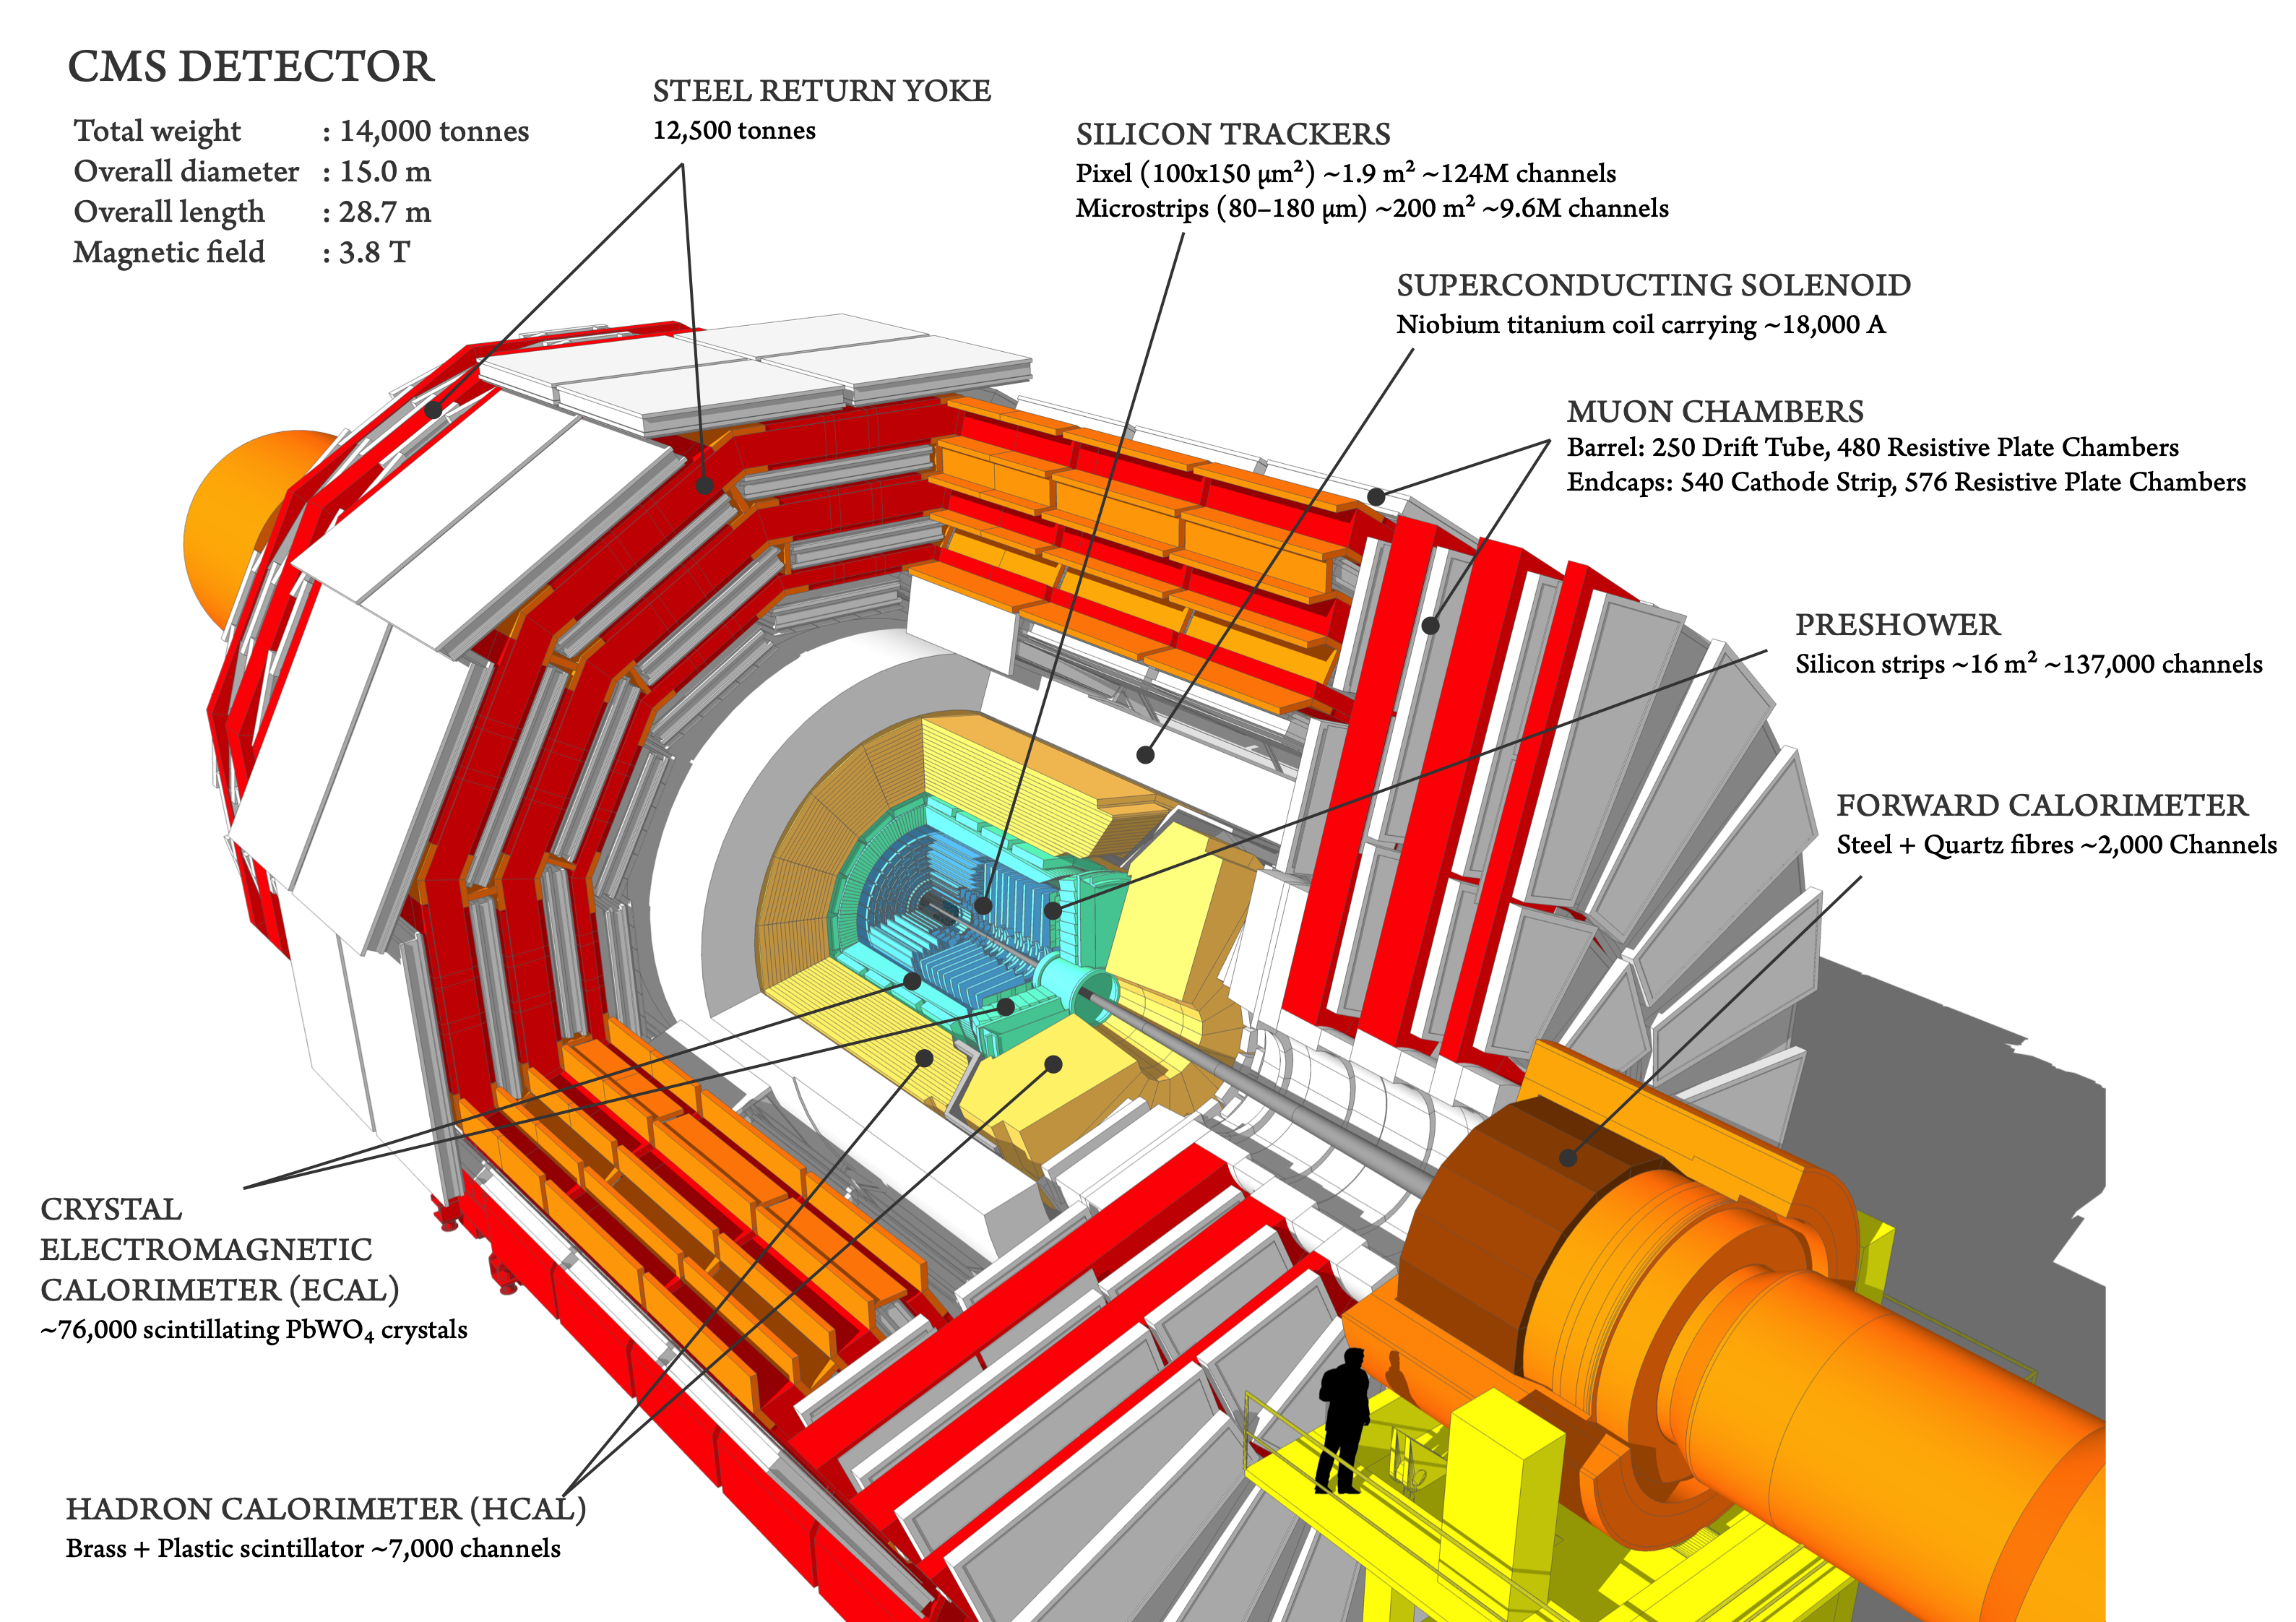
\includegraphics[width=1.0\textwidth]{figures/chapter02/CMS_160312_06.png}
    \bicaption{\quad \centering CMS探测器剖视图~\cite{Sakuma:2665537}}{\quad \centering A cutaway diagram of the CMS detector~\cite{Sakuma:2665537}}
    \label{fig:c02f03}
\end{figure}

当对撞发生时,两束在LHC环形束流管道内沿着相反方向运动的质子束流在探测器两端的磁铁作用下聚集到探测器中心并发生对撞。在完全设计的亮度下,LHC的两束质子束流都将包含2808个质子束团,其中每个质子束团都含有~\num{1.15e11}个质子,每次对撞的时间间隔为25~\si{\nano\second}。但是由于用于注射束流的磁铁在切换激活和停用的状态时存在一定时间间隔,实际的对撞次数为每秒3160万次。每次对撞平均会产生20次质子-质子相互作用,在电弱尺度下,这些散射都是由每个质子的夸克或者胶子所引发的,因此实际的对撞能量会小于束流的质心能量。在这20次的相互作用中,但绝大多数相互作用顶点都会发生弹性散射,而只有一小部分的相互作用顶点会发生非弹性散射并产生我们感兴趣的物理过程。

对撞产生的末态粒子在经过各层探测器后会被各子探测器所响应,最终重建为一个一个单独的粒子。重建出来的粒子在探测器中的位置可以用赝球面坐标系($r,\eta,\phi$)来表示,其中$r$是目标点到对撞点的距离,$\phi$是横向平面内的方位角,$\eta$是赝快度定义为$\eta = \ln{\tan{\theta/2}}$,其中$\theta$为目标点与束流方向的极角。在CMS实验中,粒子的四动量通常表述为($\pt,\eta,\phi,m$),其中$\pt$表示粒子的动量在横向的投影;$m$为粒子的质量。

在2012年CMS和ATLAS共同宣布发现希格斯粒子之后,标准模型的最后一块拼图被找到,CMS也完成了它建立之初最重要的一个物理目标。目前,CMS探测器作为一个大型通用粒子物理探测器,现在的物理目标主要有:在~\si{\TeV}级别探寻新物理;在希格斯粒子被发现后,更进一步的研究它的性质;寻找超出标准模型新物理的证据,包括超对称和额外维;研究重离子对撞。

\subsection{硅径迹探测器}

在探测器中,动量是描述一个粒子的重要信息,它对构建对撞发生时的物理过程具有至关重要的作用。由于运动的带电粒子在磁场中会受到洛伦兹力的作用,当磁场处于均匀恒定的状态时,带电粒子受到的作用力方向垂直于粒子运动方向和磁场方向。这时,带电粒子在垂直于磁场的平面上做匀速圆周运动,又称拉莫尔运动,匀速圆周运动的半径又称拉莫尔半径。根据粒子做匀速圆周运动以及受到的向心力为洛伦兹力,计算可得拉莫尔半径的表达式为:
\begin{equation}\label{eq:2-1}
    r_{g}=\frac{m v_{\perp}}{|q| B}
\end{equation}
其中,$m$为粒子质量,$v_{\perp}$为粒子垂直于磁场方向的速度,$q$是粒子的带电荷量,$B$是磁场强度。由此我们可以看出,在磁场恒定的条件下,可以通过测量粒子的回转半径(即拉莫尔半径)来计算出粒子的动量。硅径迹探测器正是通过记录带电粒子在探测器中的几个关键位置来重建出粒子轨迹,进而通过轨迹的回转半径计算出粒子的动量。

正如名称所言,CMS实验的径迹探测器完全由硅制成,包括位于探测器核心的硅像素探测器和包裹在外围的硅微条探测器,可以重建出高能缪子、电子、强子以及来自寿命非常短的粒子(比如b夸克)衰变的轨迹。由于需要精确测量粒子的位置信息同时尽可能小干扰粒子的运动轨迹,利用尽可能少的层数精确测量粒子的位置信息成为了关键。

\begin{figure}[!htbp]
    \centering
    %trim option's parameter order: left bottom right top
    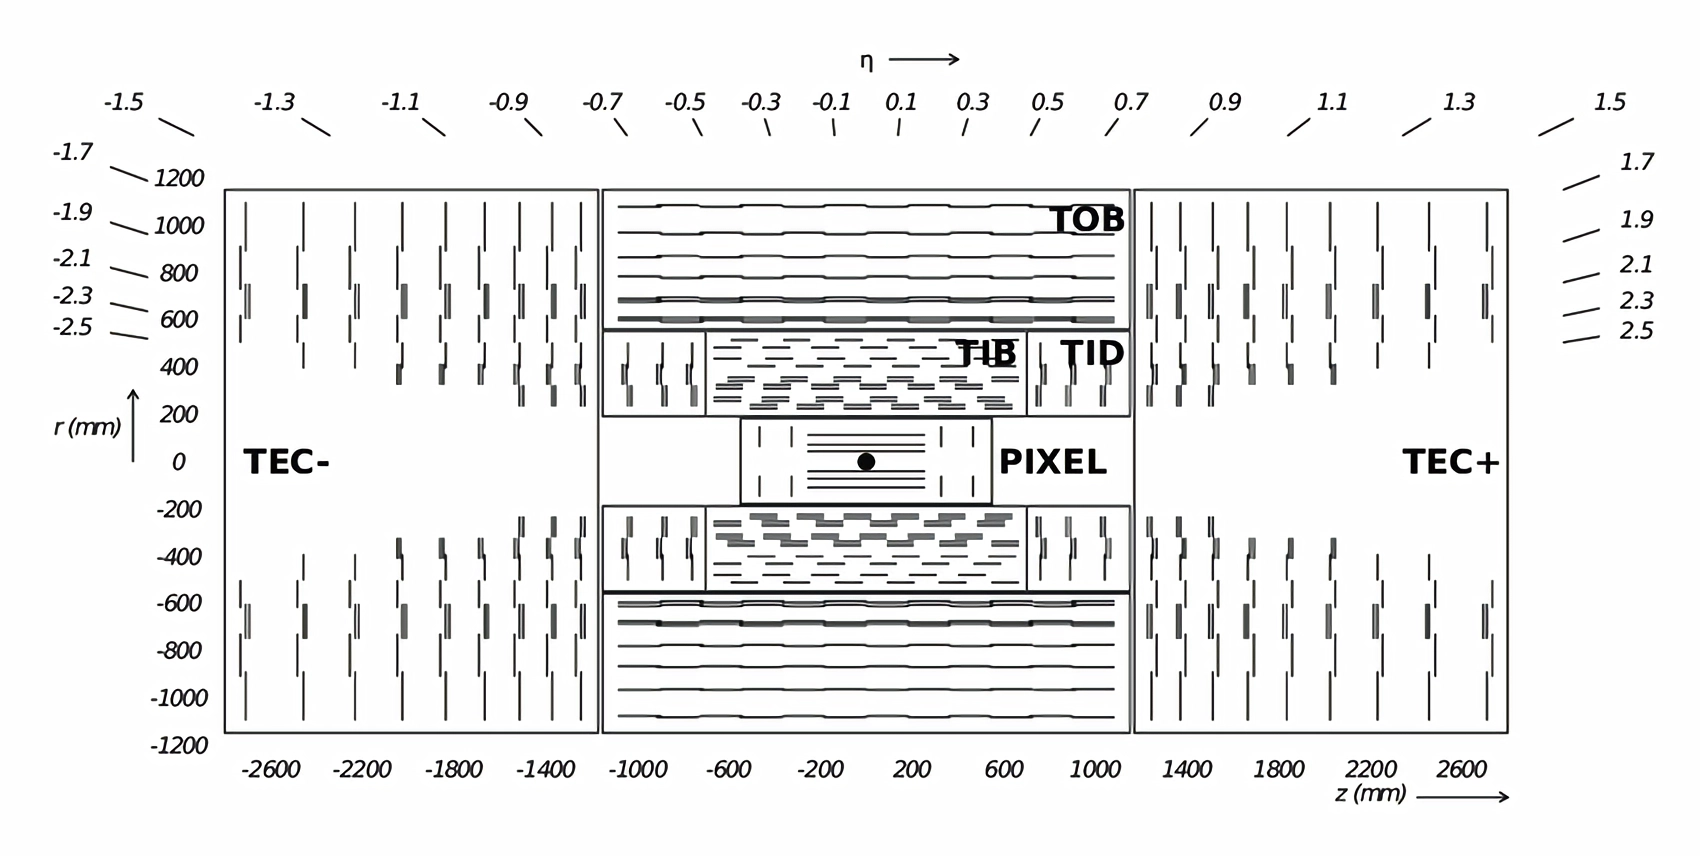
\includegraphics[width=1.0\textwidth]{Thesis (Version 2246)/figures/chapter02/Schematic-cross-section-of-the-CMS-tracker-Each-line-represents-a-detector-module.png}
    \bicaption{\quad \centering CMS径迹室示意图~\cite{Bauer:1308713}}{\quad \centering Schematic overview of the CMS tracker~\cite{Bauer:1308713}}
    \label{fig:c02f04}
\end{figure}

目前,CMS实验上的径迹探测器如图~\ref{fig:c02f04}所示,包含桶部区域的14层和端盖区域的15层探测器。它对粒子的位置测量可以精确到10~\si{\micro\meter},只有人类头发丝的十分之一。最里面的四层由100~\si{\um} $\times$ 150~\si{\micro\meter}的硅像素探测器组成,一共1.24亿个像素;剩下的均由硅微条探测器组成,包括中间四层10~\si{\centi\meter} $\times$ 180~\si{\micro\meter}的硅微条探测器以及外围六层25~\si{\centi\meter} $\times$ 180~\si{\micro\meter}的硅微条探测器,一共包含960万个硅微条探测器。当粒子经过径迹探测器时,会在探测器内部产生微弱的电信号,经过放大后的信号会被后端电子学所接收并用于粒子径迹重建。



\subsection{晶体电磁量能器}

在CMS实验中,粒子的能量对重建对撞物理过程也具有非常重要的意义。电磁量能器(ECal)的作用主要是精确测量电子和光子的能量以及沉积位置。它是由钨酸铅晶体(PbWO$_{4}$)所构成,这种物质密度非常高但是却具有光学透明性,设计目的是利用电磁簇射吸收高能粒子的能量使其沉积在探测器中并测量其能量。由于其高透明性,当电子或光子经过探测器时会使其发生闪烁,闪烁光的强度与粒子的能量成正比,通过雪崩放大后的闪烁光被后端电子学所接收并用于重建粒子的能量。选用这种材料的优势是它产生的闪烁光具有非常快的光输出,可以在一次对撞的时间内(25~\si{ns})内完成80\%的光输出。

\begin{figure}[!htbp]
    \centering
    %trim option's parameter order: left bottom right top
    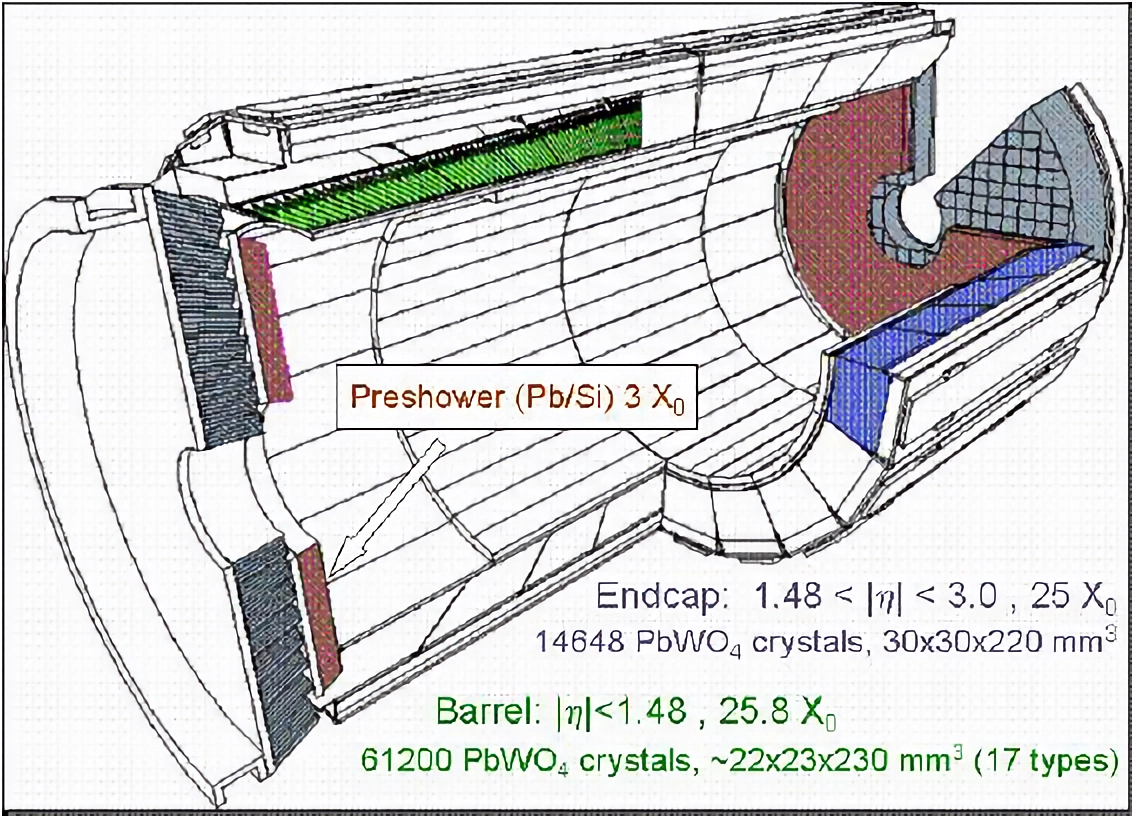
\includegraphics[width=0.8\textwidth]{figures/chapter02/View-of-the-CMS-electromagnetic-calorimeter.png}
    \bicaption{\quad \centering CMS电磁量能器外观图~\cite{ECAl}}{\quad \centering View of the CMS electromagnetic calorimeter~\cite{ECAl}}
    \label{fig:c02f05}
\end{figure}

目前在CMS实验上所使用的晶体电磁量能器的结构如图~\ref{fig:c02f05}所示 。在桶部区域,一共含有61200个晶体,每个晶体的尺寸约为22~\si{mm} $\times$ 23~\si{mm} $\times$ 230~\si{mm},构成36个超级模块;每个模块包含1700个晶体,重约三吨。端盖部分一共含有4648个晶体,尺寸为30~\si{mm} $\times$ 30~\si{mm} $\times$ 220~\si{mm}。为了增加额外的空间辨别精度,电磁量能器也包含了位于端盖前部的预簇射探测器(preshower detector),它的作用主要是探测小角度的单个高能光子或者低能光子对。

\subsection{强子量能器}

除了电子和光子的能量,重建最初对撞的物理过程也需要强子的能量信息,强子量能器(HCal)正是用于测量强子能量的探测器,其结构图如图~\ref{fig:c02f06}所示。强子量能器是由多层致密材料(黄铜或者钢)和塑料闪烁体交错组成的,这种设计的目的是为了使得磁铁线圈内的材料具有最大的能量吸收率,其中致密材料用于吸收强子的能量、塑料闪烁体用于测量粒子的能量。目前,CMS实验上的强子量能器主要有四部分:桶部部分(HB)、端盖部分(HE)、外围部分(HO)以及前向部分(HF)。

\begin{figure}[!htbp]
    \centering
    %trim option's parameter order: left bottom right top
    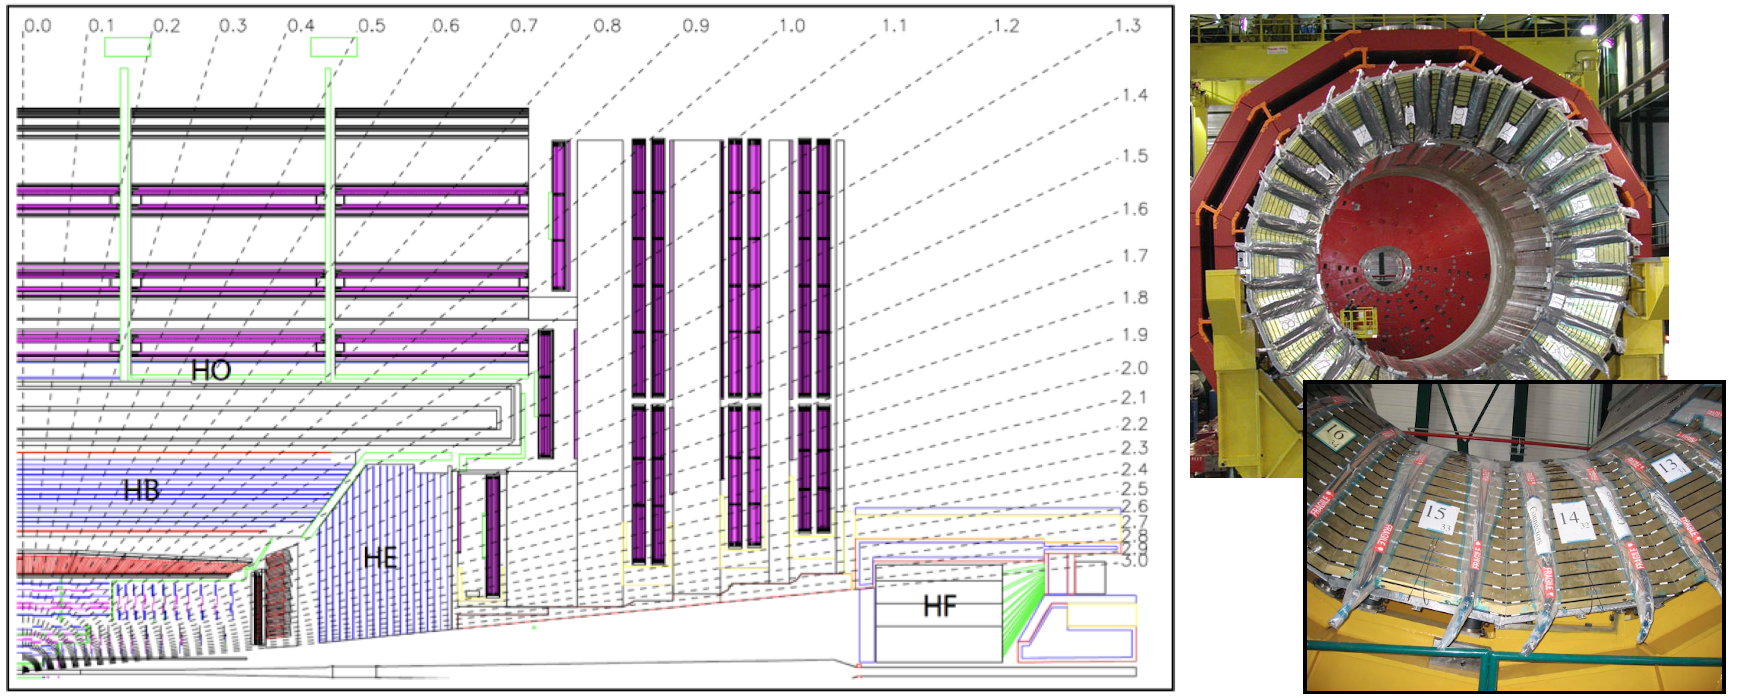
\includegraphics[width=1.0\textwidth]{figures/chapter02/hcal.png}
    \bicaption{\quad \centering CMS强子量能器示意图~\cite{phdthesis}}{\quad \centering Schematic diagram of CMS hadron calorimeter~\cite{phdthesis}}
    \label{fig:c02f06}
\end{figure}


桶部的强子量能器一共包含2304个探测器模块,每个模块所覆盖的方位角为$\Delta\eta\times\Delta\phi = 0.087\times0.087$,总共覆盖了赝快度为$-1.4<\eta<1.4$的区域。

对于端盖部分,探测器模块覆盖了赝快度为$1.3<|\eta|<3.0$的区域,总共含有2304个模块,其中最外围的5层探测器每个模块$\phi$角度覆盖范围为5\si{\degree},$\eta$角度覆盖范围为0.087;内部的8层探测器每个模块$\phi$角度覆盖范围为10\si{\degree},$\eta$角度覆盖范围为0.09到0.35。

强子量能器的外围部分主要是由10~\si{mm}厚的闪烁体探测器所构成,位于线圈外部真空罐的外围,覆盖范围为$-1.26<\eta<1.26$。它们主要的作用是对泄漏出强子量能器的强子簇射进行采样,能够在对能量分辨函数进行测量的过程中减小尾巴部分的贡献,并且提升量能器对丢失能量测量的分辨率。

强子量能器的前向部分主要覆盖了$3.0<|\eta|<5.0$的范围,与其他部分不同,前向量能器的材料由钢和石英纤维所组成。原因是强子簇射的中性部分更倾向于被前向量能器所接收,这种设计产生的强子簇射会更窄和更短,因此更适合簇射环境比较拥挤的前向部分。前向量能器位于对撞顶点11.2米处,吸收体深度为1.65米,信号来源于粒子穿过石英纤维时发出的切伦科夫光,经过光电倍增管放大后被后端电子学接收。

\subsection{磁铁系统}

CMS实验的磁铁系统如图~\ref{fig:c02f07}所示,是由一个长约12.5米、内孔直径约5.9米的超导螺线圈组成,它最大可以产生4特斯拉的超强磁场,是地球磁场的10万倍,但为了最大程度的延长磁铁的使用寿命,实际运行中产生的磁场为3.8特斯拉。这使得我们可以根据带电粒子在磁场中的弯曲轨迹来确定粒子的荷质比,进而来辨别粒子种类。

\begin{figure}[!htbp]
    \centering
    %trim option's parameter order: left bottom right top
    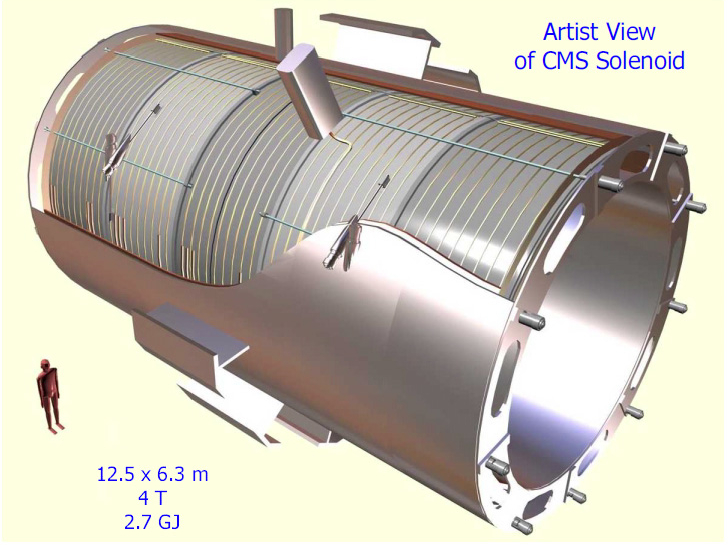
\includegraphics[width=0.8\textwidth]{figures/chapter02/CMS-solenoid-magnet.jpeg}
    \bicaption{\quad \centering CMS螺线管磁铁~\cite{Magnet}}{\quad \centering CMS solenoid magnet~\cite{Magnet}}
    \label{fig:c02f07}
\end{figure}

径迹室、电磁量能器和强子量能器都位于螺线管内部,缪子探测器围绕着螺线管排布在外围。与此同时,巨大的磁铁也为整个实验提供了绝大多数的结构支撑。

\subsection{缪子探测器}\label{sec:MuonDetector}

正如CMS实验的名称“紧凑型缪子探测器”所提到的,探测缪子是CMS实验中最重要的目标之一。在希格斯粒子的研究中,四个缪子末态对精确测量希格斯粒子的质量和宽度起到了至关重要的作用。缪子探测器的主要目标是通过记录缪子的飞行轨迹来测量缪子的动量。

缪子是带电粒子,电荷量和电子相同,但是质量却是电子的200倍。不像其他粒子会被量能器所吸收,缪子和其他物质的相互作用非常微弱,通常可以穿过整个探测器到达探测器外围甚至飞出整个探测器。因此,缪子探测器被摆放在整个CMS探测器最外围,只有缪子是唯一可能产生信号的来源。

\begin{figure}[!htbp]
    \centering
    %trim option's parameter order: left bottom right top
    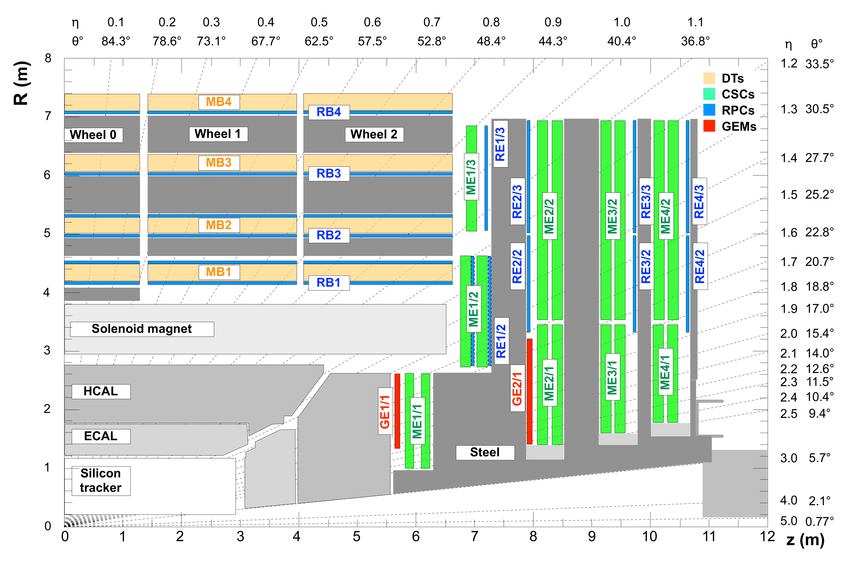
\includegraphics[width=0.8\textwidth]{figures/chapter02/Quadrant-of-the-CMS-detector-showing-the-present-muon-system-including-RPCs-DTs-and.png}
    \bicaption{\quad \centering CMS缪子系统~\cite{MuonSystem}}{\quad \centering CMS Muon system~\cite{MuonSystem}}
    \label{fig:c02f08}
\end{figure}

目前运行在CMS实验上的缪子探测器如图~\ref{fig:c02f08}所示,主要由四部分探测器所组成:漂移管道室(DT)、阴极条形室(CSC)、电阻板室(RPC)和气体电子倍增器(GEM)。DT用于精确测量桶部的缪子轨迹;而CSC用于端盖的缪子轨迹测量;RPC可以在缪子通过探测器时提供快速的信号响应,因此同时被安装在了桶部和端盖。这四种探测器都属于气体探测器,密闭的空间中充入介质气体,并且包含一个阳极面和阴极面。当缪子或者任何带电粒子经过探测器时,会使气体发生电离并将气体中原子的核外电子剥落,这些电子会随着电场的方向漂移到阳极丝,阳离子会漂向阴极板,最终被前端电子学所收集成为信号。

漂移管道室(Drift Tube chamber, DT)的结构如图~\ref{fig:c02f09}所示,它是一种气体漂移室,每根4厘米宽的气体管子中间包含有一根拉伸的金属丝,气体介质为Ar和CO$_2$的混合气体。每个漂移管道室的平均尺寸为2~\si{m} $\times$ 2.5~\si{m},由12层铝层构成,分为三组,每组四个,每层最多由60个漂移管道所构成;三组中中间一组测量平行于束流方向的坐标,另外两组测量垂直于束流方向的坐标。

\begin{figure}[!htbp]
    \centering
    %trim option's parameter order: left bottom right top
    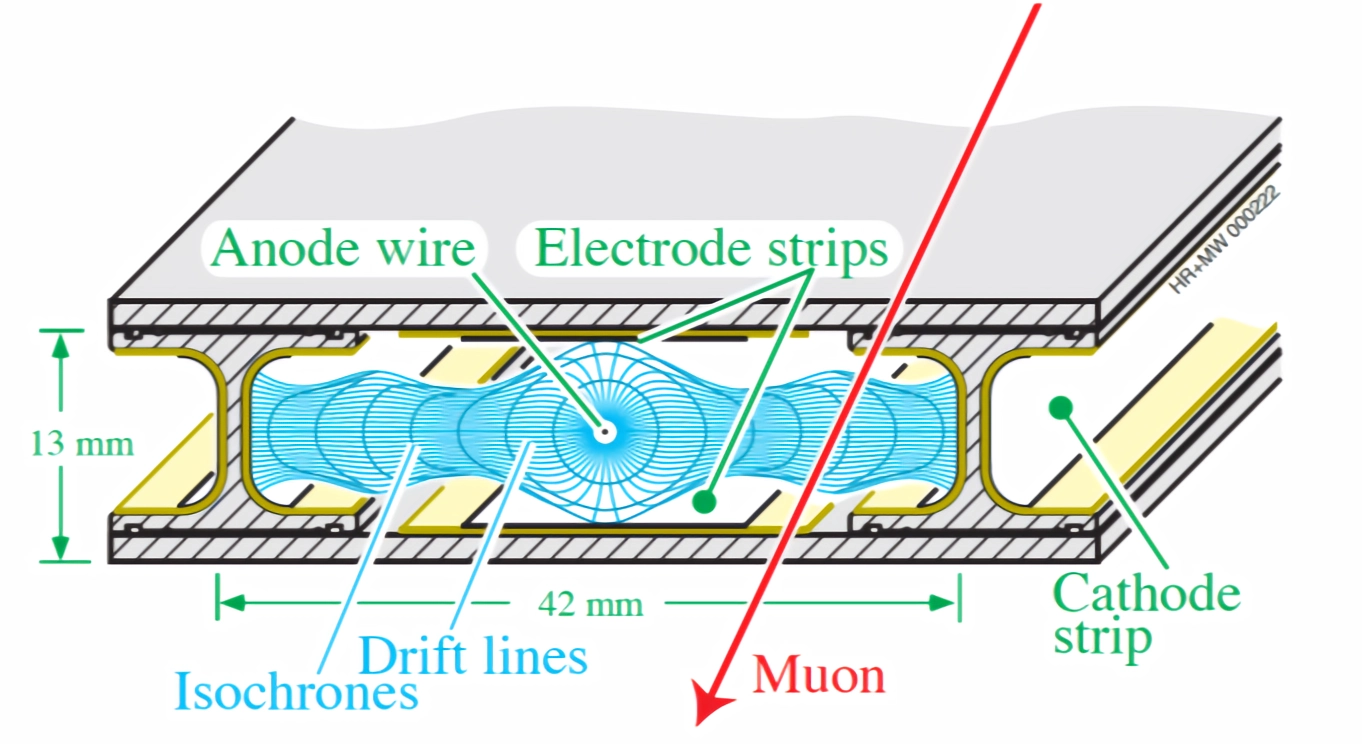
\includegraphics[width=1.0\textwidth]{Thesis (Version 2246)/figures/chapter02/DT.png}
    \bicaption{\quad \centering DT探测器示意图~\cite{Guiducci:1027479}}{\quad \centering Schematic view of the DT detector~\cite{Guiducci:1027479}}
    \label{fig:c02f09}
\end{figure}

阴极条形室(Cathode strip chambers, CSC)的结构如图~\ref{fig:c02f10}所示,每个探测器由六层宽度为9.5~\si{mm}的气体漂移室组成,每层都是由位于中间的阳极丝和位于两边的阴极条形板所组成,它们呈垂直方向。每根阳极丝之间的距离为3.12\si{mm},每根阴极条之间相距3.16~\si{mm},气体由50\%的CO$_2$、40\%的Ar和10\%的CF$_4$混合组成。当缪子穿过探测器时,会使探测器中的气体分子发生电离,在外置电场的作用下,电离产生的电子被雪崩放大,最终运动到阳极丝附近被吸收,使得阳极前端板(Anode Front End Board, AFEB)接收到信号;与此同时,电离产生的阳离子在电场的作用下漂移到阴极板,使得阴极前端板(Cathode Front End Board, CFEB)接收到信号。将AFEB和CFEB中的信号进行配对匹配,就可以确认是否信号真正来源于缪子所产生的击中。目前CMS实验上两个端盖部分的CSC探测器均由四个大圆形环所构成,一共有540个阴极条形室。由于阳极丝和阴极条形板之间互相垂直,CSC探测器可以测量粒子的二维坐标;此外,由于紧密排列的电线使得CSC探测器能够快速的探测粒子经过的信号,这使得CSC探测器也成为了触发系统的一部分。

\begin{figure}[!htbp]
    \centering
    %trim option's parameter order: left bottom right top
    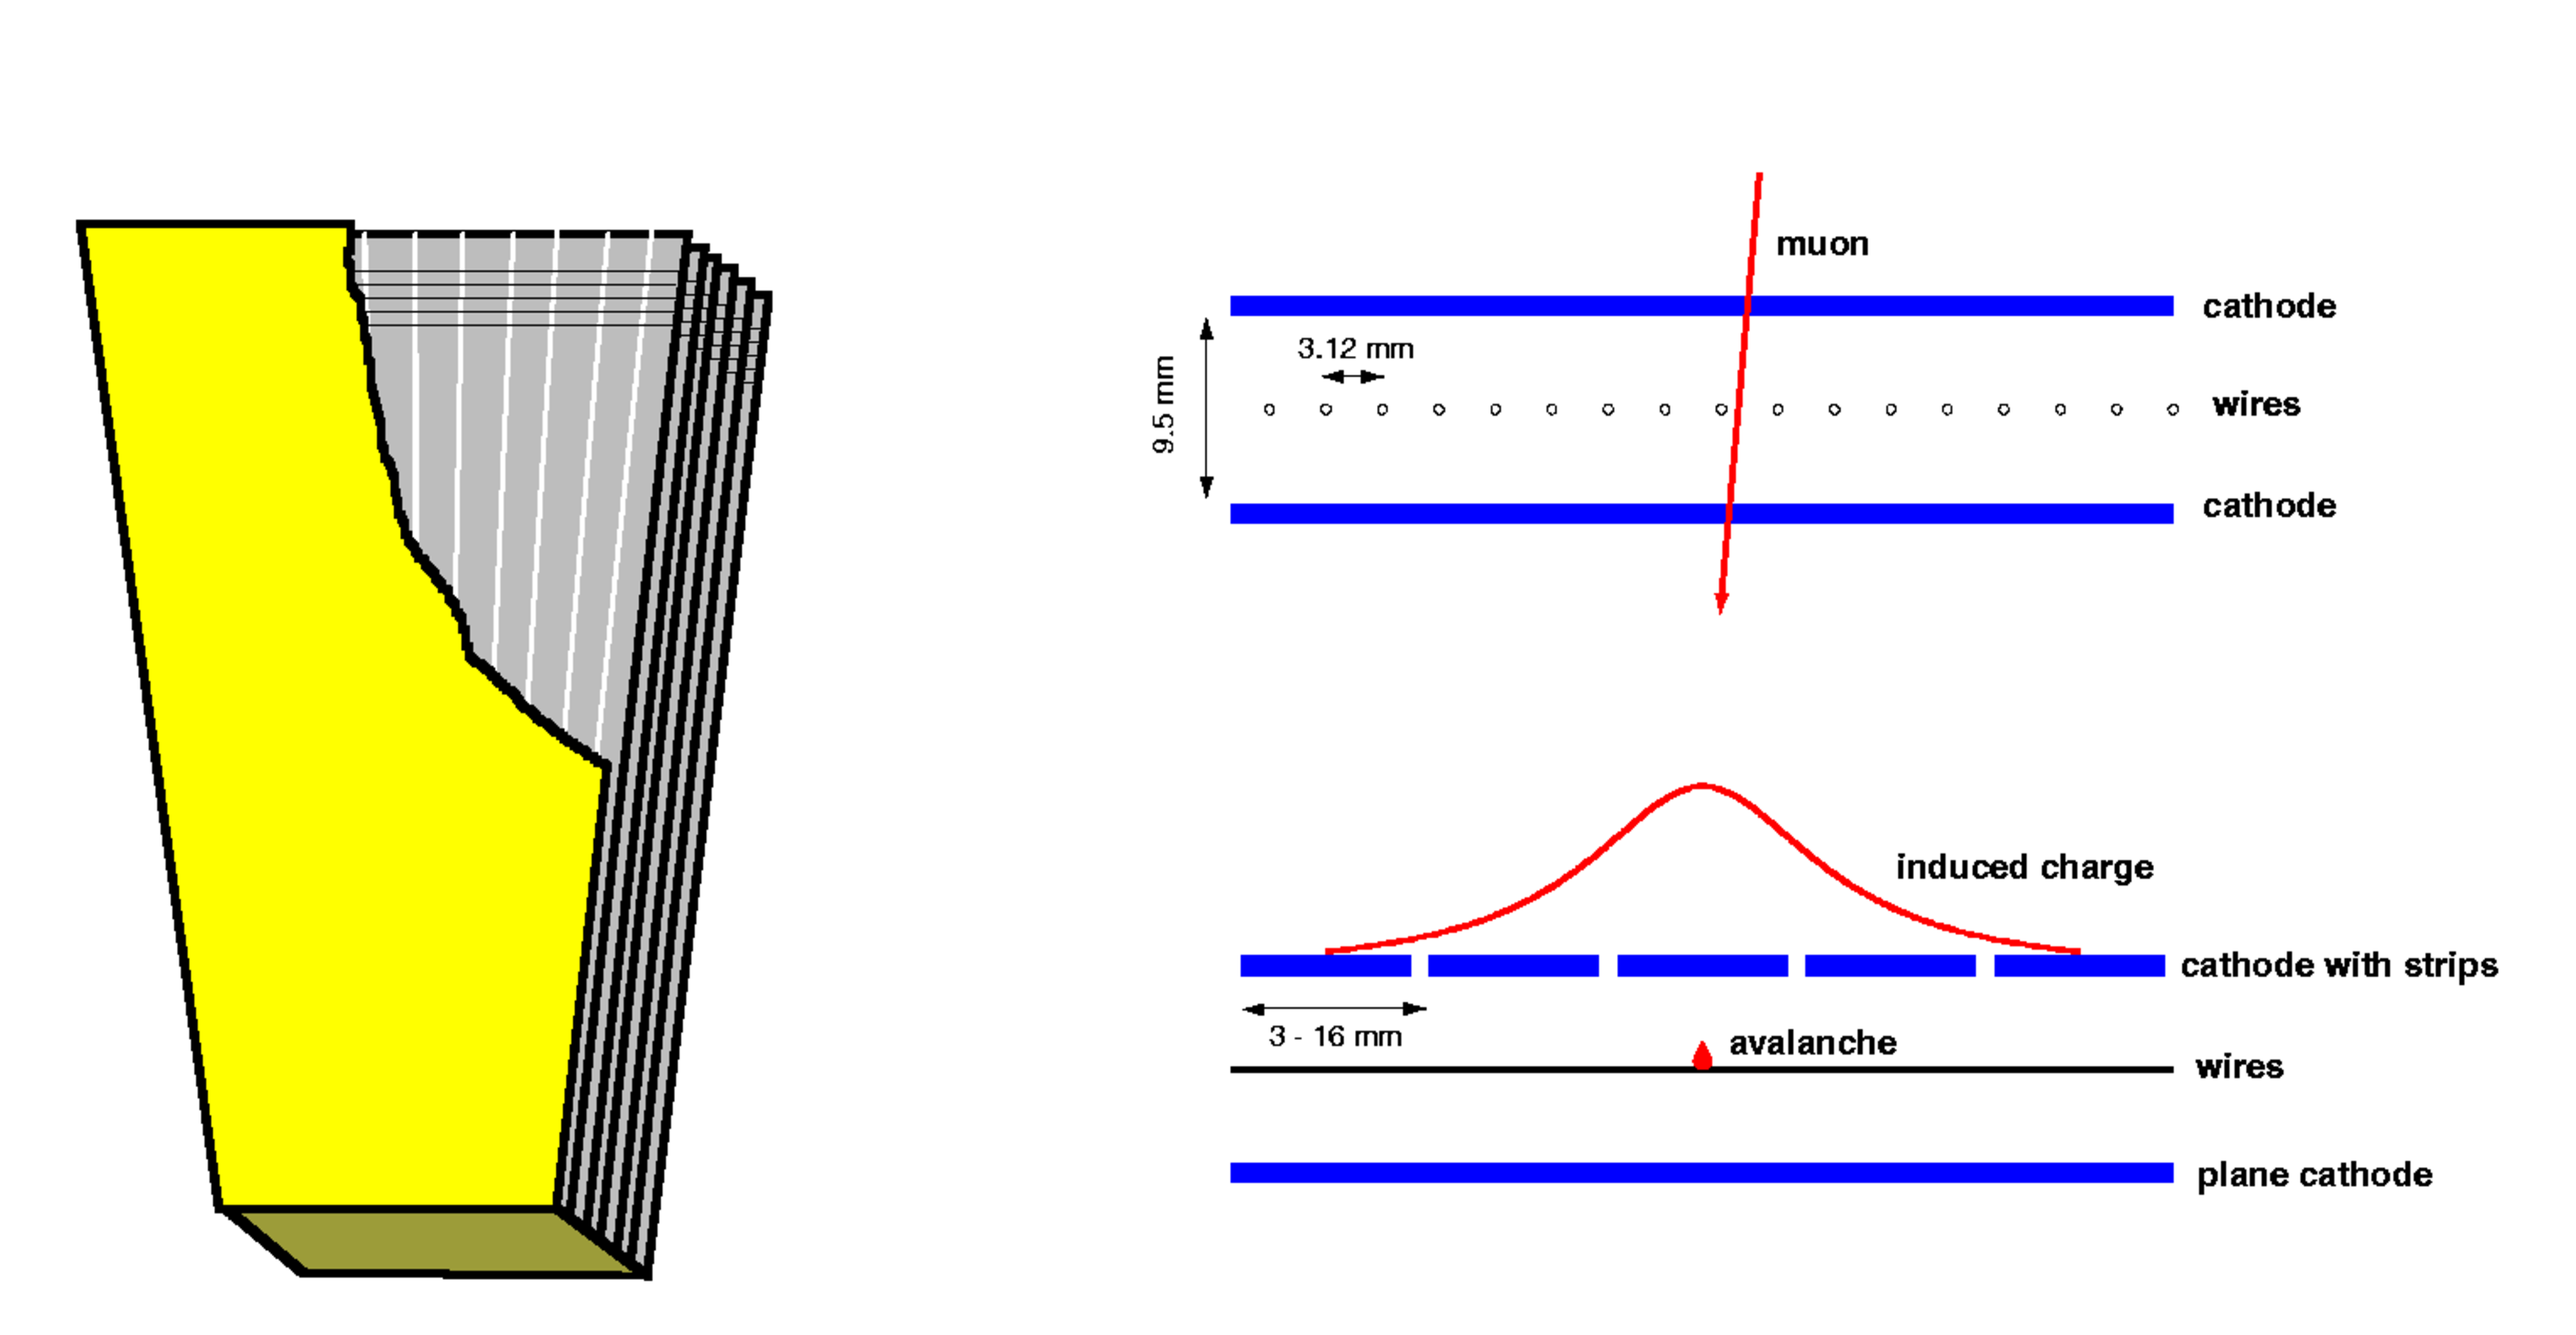
\includegraphics[width=0.8\textwidth]{Thesis (Version 2246)/figures/chapter02/CSC.pdf}
    \bicaption{\quad \centering CSC探测器示意图~\cite{CSC}}{\quad \centering Schematic view of the CSC detector~\cite{CSC}}
    \label{fig:c02f10}
\end{figure}

电阻板室(Resistive plate chambers, RPC)的结构如图~\ref{fig:c02f11}所示,它由两个平行的平面所构成,一个是带正电的阳极板,另一个是带负电的阴极条形板,它们都是由电阻率非常高的塑料材料所制成,中间用气体隔开。RPC探测器具有非常好的空间辨别率以及仅为1~\si{ns}的时间分辨率,使得它可以作为与DT和CSC探测器互相平行的缪子触发系统。

\begin{figure}[!htbp]
    \centering
    %trim option's parameter order: left bottom right top
    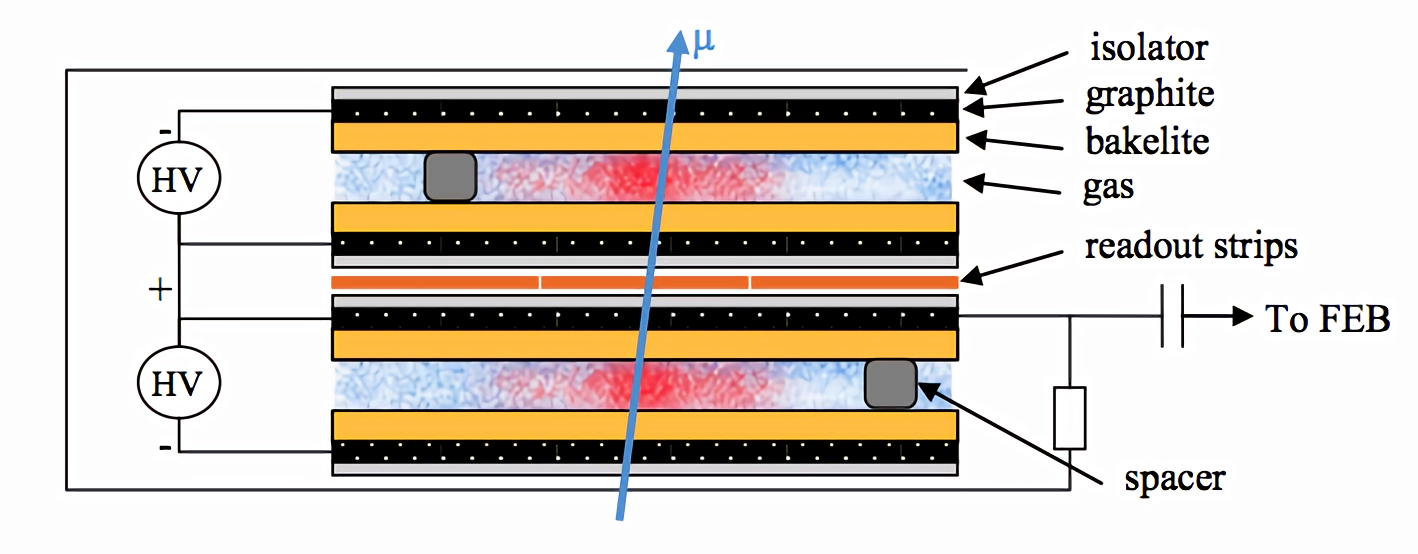
\includegraphics[width=1.0\textwidth]{figures/chapter02/rpc-schema.png}
    \bicaption{\quad \centering RPC探测器示意图~\cite{RPC}}{\quad \centering Schematic view of the RPC detector~\cite{RPC}}
    \label{fig:c02f11}
\end{figure}

气体电子倍增器(Gas electron multiplier, GEM)是运行在CMS实验上新的缪子探测系统,它们是LHC在2阶段停机升级期间安装完成的,主要目的是补充端盖现有的缪子探测系统。由于端盖区域是CMS探测器受到辐射最大和事例率最高的区域,GEM探测器可以提供额外的测量点,从而可以获得更好的缪子径迹辨别以及更大范围的端盖覆盖区域。GEM探测器的结构如图~\ref{fig:c02f12}所示,它是由三层50~\si{um}厚的覆铜聚酰亚胺箔所构成,中间充满了Ar和CO$_2$的混合气体。

\begin{figure}[!htbp]
    \centering
    %trim option's parameter order: left bottom right top
    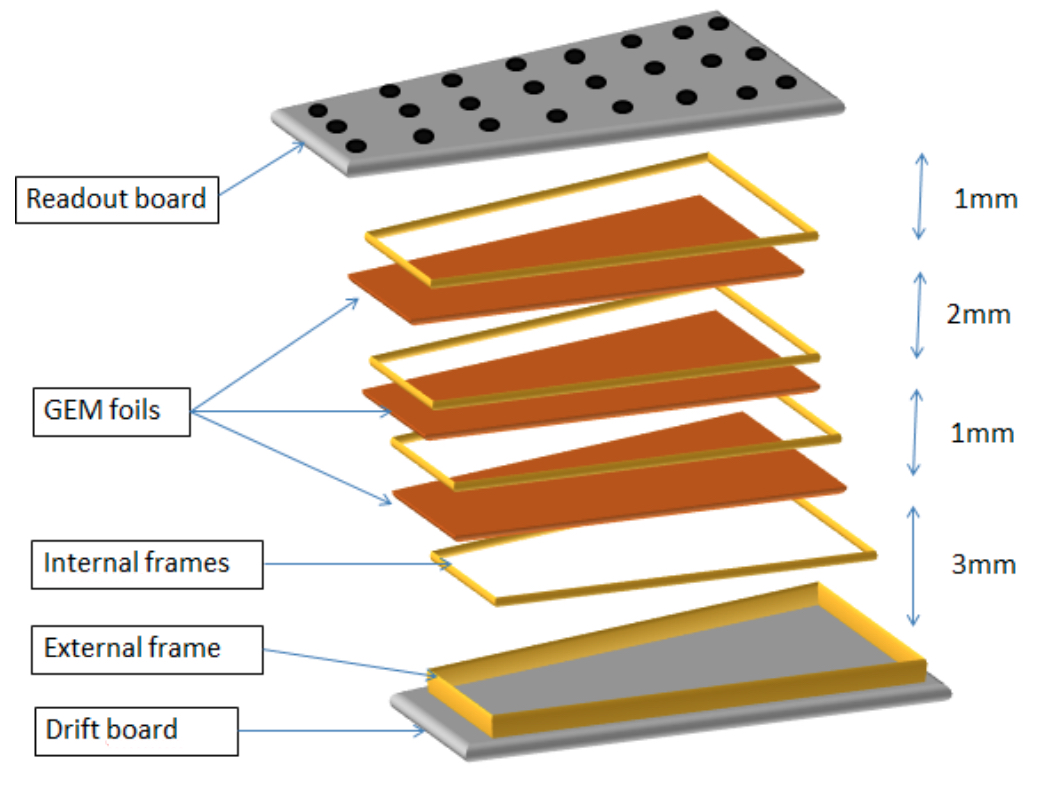
\includegraphics[width=0.6\textwidth]{figures/chapter02/GEM.jpg}
    \bicaption{\quad \centering GEM探测器示意图~\cite{CALABRIA20161042}}{\quad \centering Schematic view of the GEM detector~\cite{CALABRIA20161042}}
    \label{fig:c02f12}
\end{figure}

\subsection{触发以及数据获取}

在CMS实验中,束流对撞频率为25~\si{ns}一次,40~\si{MHz},平均每次对撞产生的原始数据量为1~MB,这就意味着每秒钟在CSM探测器中可以产生40~\si{TB}的原始数据,而这其中的绝大多数事例都是我们所不感兴趣的弹性碰撞。如此庞大的数据量不可能同时都被存储系统所记录下来,因此触发系统的作用就是尽可能快速的利用部分原始信息只过滤出我们感兴趣的事例。为了完成这个目标,在CMS实验中采用了多级触发的形式,完整的触发系统可以将每秒钟记录的事例数控制在1000个。图~\ref{fig:c02f13}展示了CMS实验的触发系统,主要由两部分构成:一级触发(Level 1 trigger)和高级触发(High Level trigger)。

\begin{figure}[!htbp]
    \centering
    %trim option's parameter order: left bottom right top
    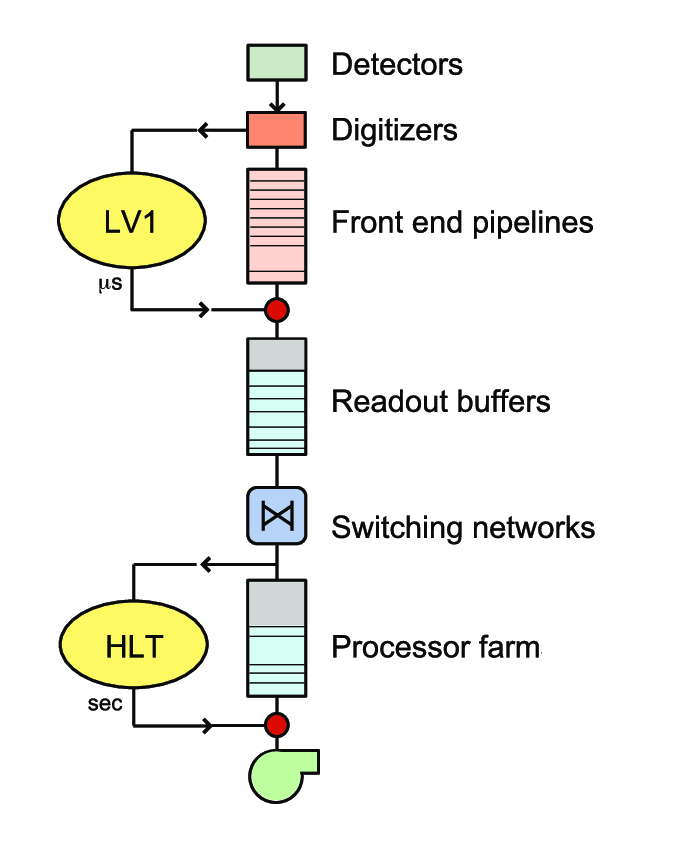
\includegraphics[width=0.6\textwidth]{figures/chapter02/trigger.png}
    \bicaption{\quad \centering CMS触发系统示意图~\cite{trigger}}{\quad \centering Schematic view of the CMS trigger system~\cite{trigger}}
    \label{fig:c02f13}
\end{figure}

对于一级触发,每次对撞的所有信息都被存储在探测器的缓存中,只有少量的关键信息被用于执行快速的、近似的计算,并用于识别我们感兴趣的特征,比如说:高能喷注、缪子或者丢失的能量。这个计算可以在大约1~\si{ns}的时间内完成,并且可以将每秒钟总的事例数降低大约1000倍,达到50~\si{kHz}。所有的这些计算都是基于硬件来完成的,因此一级触发也称为硬件触发。

对于通过一级触发的事例,缓存在探测器中的对撞数据将通过光纤链路传递给高级触发。高级触发通常指的是运行在计算机服务器上的软件,因此也称为软件触发。由于经过一级触发后到达高级触发的事例数发生了明显降低,这就使得高级触发有足够多的时间进行更加详细的分析。最终,通过高级触发的事例数可以再降低100倍,达到每秒钟1000个事例,这些事例作为我们感兴趣的事例最终被存储到磁带上并用于之后的物理分析。
%%% Local Variables: 
%%% mode: latex
%%% TeX-master: t
%%% End: 

\chapter{CMS事例模拟与重建}

\section{CMS事例模拟}

质子-质子对撞相比于正负电子对撞最大的优势就是对撞中心能量可以非常高,但是与此同时,质子-质子对撞也有明显的劣势:本底环境非常复杂。在电弱尺度下,发生对撞的主要是质子中的夸克和胶子,而质子内部含有非常多的胶子和夸克,这就使得对撞发生时会有非常多的本底,对我们所要寻找的物理过程产生严重阻挠。因此,理解对撞数据中的本底事例对最终的信号提取具有至关重要的作用。与此同时,除了扣除本底外,因为对撞事例中同时包含信号事例和本底事例,但是由于统计量的原因,信号事例被淹没在本底事例之中;或者对于新物理的寻找,我们不知道它具体出现在哪里。这时,可以通过对信号的模拟与数据做对比或者拟合,来得出信号在数据中的成分。因此,事例模拟在粒子物理实验中有着至关重要的作用。

目前,CMS实验通过使用基于蒙特卡洛(Monte Carlo, MC)方法的计算机模拟来对粒子物理实验中的各个本底事例和信号事例进行模拟。由于需要详尽的模拟对撞机中发生的物理过程,模拟一共分为两个阶段,分别为物理事例的产生模拟和事例在探测器中的模拟。

物理事例的产生模拟主要用来模拟每次对撞时发生的物理过程,包括最初的硬散射过程、强子化过程以及之后的非硬散射过程模拟(underlying Event, UE)。这些模拟可以通过不同的产生子来实现,比如:Madgraph~\cite{alwall2014automated},Herwig~\cite{bellm2016herwig},Pythia~\cite{sjostrand2008brief},Sherpa~\cite{gleisberg2009event},POWHEG~\cite{alioli2010general}。通过模拟我们可以得到产生子级别的事例信息,而后这些信息将用于模拟粒子在探测器中的响应。

探测器模拟主要用于模拟对撞产生的粒子在探测器中的响应,包括模拟事例在探测器中的运动轨迹、沉积能量以及与探测器物质发生相互作用后的情形等等。目前,CMS实验所使用的探测器模拟是基于GEANT4~\cite{agostinelli2003geant4}的软件框架,模拟包括了CMS探测器的所有子探测器以及构成探测器的其他成分。

\section{CMS事例重建}

在事例通过触发的选择后,存储下来的原始数据包含了粒子在各个子探测器中的响应,这些数据本身只是一些电子学信号,并不能够直接用于物理分析。但是,由于不同的粒子在整个探测器中留下的电子学信号不同,可以根据这些信号重建出最初的物理对象,比如:光子、电子、缪子和强子喷注,这种重建方法被称为粒子流算法(particle-flow algorithm, PF)。

如图~\ref{fig:c03f01}所示,粒子流算法的主要目的是结合各个子探测器的信息重建出对撞事例中的稳定粒子,比如电子、光子、缪子以及比较稳定的强子,算法优化了对粒子的种类、方向和能量的辨别。而后,这些稳定的粒子被用来重建更高阶的物理对象,比如喷注、$\tau$子、丢失的横向能量(missing transverse energy);也可以用来计算带电轻子或者光子的隔离度(isolation)等等。

\begin{figure}[!htbp]
    \centering
    %trim option's parameter order: left bottom right top
    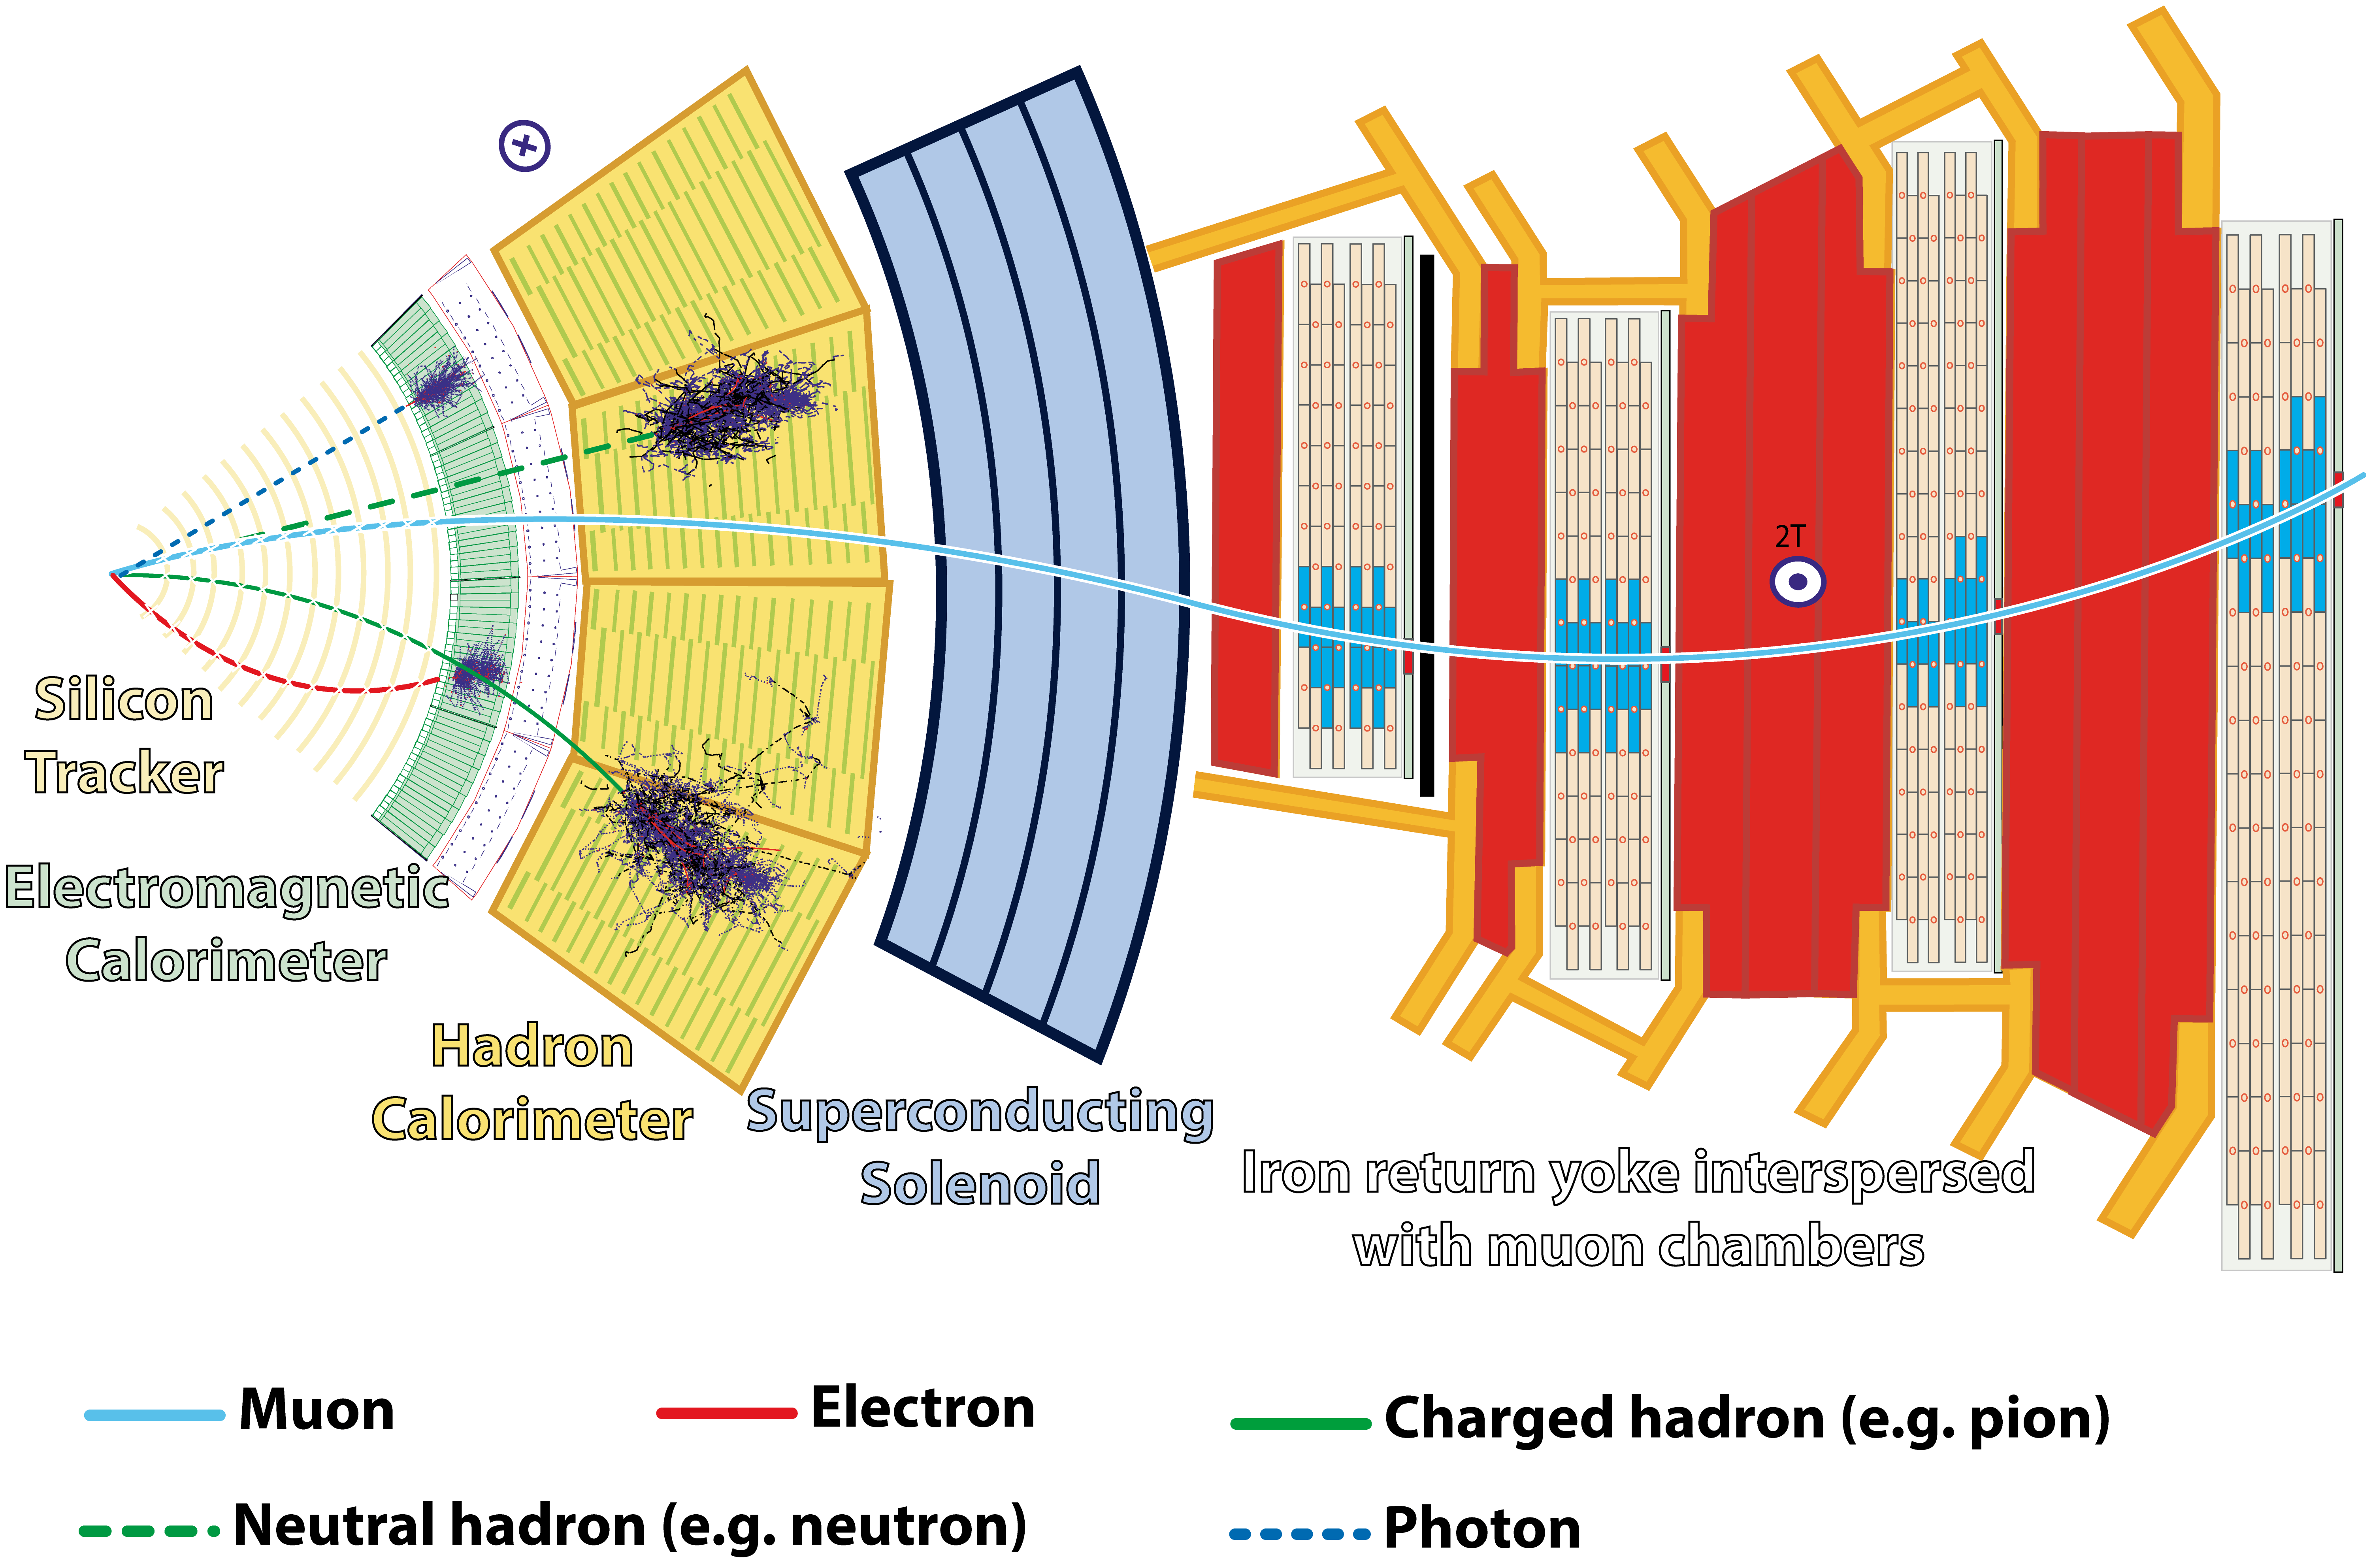
\includegraphics[width=0.6\textwidth]{figures/chapter03/CMSslice_whiteBackground.png}
    \bicaption{\quad \centering 不同粒子在探测器中的响应~\cite{Barney:2120661}}{\quad \centering Responses of different particles in the detector~\cite{Barney:2120661}}
    \label{fig:c03f01}
\end{figure}

粒子流算法重建事例的基本元素包括中心径迹探测器内重建出的对撞顶点和带电粒子的轨迹、电磁量能器和强子量能器中重建出来的能量簇射以及缪子探测器中重建出的缪子轨迹。带电粒子的轨迹是利用迭代跟踪的策略重建出来的,对于动量高达150$\GeV$的带电粒子,粒子流算法仍然可以同时保持非常高的效率和非常低的误判率。能量簇射是在各个量能器子探测器中利用专门的簇射算法构建出来的,这个算法是专为粒子流算法所设计,主要目的是为了可以对低能粒子和能量沉积相距比较近的粒子保持比较高的探测效率。而后,这些基本元素通过连接算法连接起来用于完整的重建出单个粒子,同时删除不同子探测器中可能出现的重复计数。

对于光子和电子的辨别,这两者在探测器中的响应非常相似,都可以被电磁量能器所吸收并测量其能量,而且这两者在电磁量能器中的簇射形状也十分类似,但是由于光子不带电荷而电子带电荷,使得电子可以在中心的径迹探测器内留下轨迹并且在磁场的作用下发生偏转,而光子不会在径迹探测器内留下轨迹。因此,粒子流算法通过辨别在电磁量能器中沉积能量的粒子是否同时在中心径迹探测器中留下轨迹来辨别出电子和光子。强子喷注主要是由对撞产生的夸克和胶子在探测器中的强子化过程所产生。对于带电的夸克产生的喷注会在径迹探测器中留下径迹并被磁场所弯曲,而中性强子或者胶子只会在强子量能器中产生簇射并被探测器所接收。由于缪子和其他物质的相互作用非常弱,它会穿过强子量能器到达外围的缪子探测器并在其中留下轨迹。粒子流算法可以通过缪子探测器以及中心径迹探测器中的信号来辨别缪子。当所有的物理对象重建出来后,一部分不可探测的粒子,比如中微子,会飞出探测器,但是根据横向动量守恒,我们可以根据其它所有物理对象重建出丢失的横动量。

\subsection{径迹室轨迹和对撞顶点重建}\label{subsec:PVReco}

CMS实验中,对中心径迹室中带电粒子运动轨迹的重建依赖于对撞产生的带电粒子穿过径迹探测器时所留下的击中信息。利用这些信息,可以通过使用基于组合卡尔曼滤波法(Combinatorial Kalman filter)的“迭代追踪”的方法重建出带电粒子的轨迹。这种方法首先对比较容易辨别的轨迹进行迭代重建,它们往往对应于横动量比较高、留下的击中信息比较完整的带电粒子轨迹。而后,将这些用于重建轨迹的击中排除,剩余的轨迹仅从剩下的击中中进行重建。这种方法可以有效降低轨迹重建时击中组合的复杂度,从而可以更好的对处于比较困难的动力学区域内的轨迹进行重建。轨迹重建的具体步骤可以分为以下四步:
\begin{itemize}
    \item 首先,对轨迹种子(Seed)进行重建,这一步对轨迹参数提供了初始估计值;
    \item 其次,将最初估计的候选轨迹传递到整个径迹室,利用卡尔曼滤波的方法找出每层探测器中与之对应的击中,并且对候选轨迹进行更新;
    \item 然后,将所有确定的击中进行合并拟合;
    \item 最后,选择质量较好的轨迹并进行保存,用于之后的物理对象重建。
\end{itemize}
目前,CMS实验中对径迹室内的带电粒子的轨迹重建效率在横动量大于1$\GeV$的条件下可以达到90\%左右~\cite{Elmetenawee:2020emw}。

由于在对撞过程中,会产生除了我们所关注的硬散射过程以外的其他过程,使得每次束流对撞都会产生数量众多的堆积事例(Pileup event),在探测器中心处可以同时观测到多个对撞顶点,而其中只有一个对撞顶点是我们所感兴趣的顶点。因此,对初级对撞顶点的重建和筛选对完整重建出我们所感兴趣的物理过程具有非常重要的物理意义。

目前,CMS实验中对撞顶点的重建主要利用了在径迹探测器中重建出来的带电粒子的轨迹,它可以对每个事例中质子质子相互作用顶点的位置和不确定度进行测量。对撞顶点的具体重建步骤可以分为以下三步:
\begin{itemize}
    \item 首先,对重建出来的轨迹进行挑选,要求选中的轨迹相对于束流点(Beam spot)的中心位置的横向对撞参数小于5、轨迹在硅像素探测器中至少含有两个击中、在硅像素和硅微条探测器中一共含有至少5个击中以及每条轨迹拟合所得到的归一化$\chi^{2}$值小于20;
    \item 然后,根据所有轨迹相对于束流点在$z$方向的最短距离对来自于同一对撞顶点的轨迹进行聚类;
    \item 最后,根据所有聚类后的轨迹拟合出对撞顶点。
\end{itemize}
这一方法可以对来自同一对撞的所有顶点进行重建,包括我们所感兴趣的硬散射过程初级顶点和堆积事例顶点。而对于初级对撞顶点的选择,CMS实验利用了重建顶点所对应的轨迹信息,选择硬散射程度最高的顶点作为初级对撞顶点。

\subsection{电子和光子的重建}\label{subsec:EGReco}

电子和光子的簇射会在电测量能器的几个晶体中沉积能量,大约94\%的能量可以沉积在3$\times$3的晶体块中,而5$\times$5的晶体块可以沉积大约97\%的能量。通过对沉积在这些晶体矩阵块中的能量进行求和,可以得出电子或光子的能量。但是由于电磁量能器内部其他物质的存在,使得电子会发生韧致辐射,光子会转换为正负电子对。在强磁场的作用下,到达量能器的能量会在$\phi$角度发散,对于这部分能量,CMS实验采取了超聚类算法(super-cluster, SC)对其进行重建。

簇射的位置信息可以通过计算簇射中晶体的能量加权平均位置得到。但是对于远离簇射核心的晶体,沉积能量相比于核心能量会呈指数下降的趋势,因此简单的能量加权平均位置给出了偏向于能量核心的位置。为了减小偏差,可以采用晶体能量的对数作为权重值。具体表达式为
\begin{equation}
    x=\frac{\Sigma x_{i} \cdot W_{i}}{\Sigma W_{i}}
\end{equation}
其中,$x_{i}$表示晶体$i$的位置,$W_{i}$是对应晶体的权重,定义为
\begin{equation}
    W_{i}=W_{0}+\log \frac{E_{i}}{\Sigma E_{j}}
\end{equation}
$W_{0}$表示偏差,$E_{i}$是晶体$i$中的沉积能量。

相比于光子,电子带有电荷,会在中心径迹室留下轨迹。因此,CMS实验利用了电子的轨迹信息对光子和电子进行了区分。但是由于韧致辐射,电子在径迹室中的轨迹由于辐射出光子而发生改变,CMS实验利用了一种非线性的滤波算法——高斯求和滤波法(Gaussian sum filter, GSF)对电子轨迹进行了重建~\cite{adam2005reconstruction},称为GSF轨迹。如果GSF轨迹和在电磁量能器中重建出来的簇射中心相匹配,这个粒子就被定义为电子;反之,就被定义为光子。

由于强子对撞机中存在复杂的本底,对撞中的堆积事例或者潜在事例(Underlying event)会产生众多的喷注,这些喷注往往会在电磁量能器中形成簇射并被误判为电子或者光子。这些假电子或着假光子会对最终的物理分析产生严重的影响。CMS实验利用了电子或者光子的各种簇射信息以及轨迹信息对真假粒子进行了区分,主要包括:
\begin{itemize}
    \item $H/E$:簇射在强子量能器中沉积的能量和电磁量能器中沉积能量的比值。
    \item $\sigma_{i\eta i\eta}$:以能量最大的晶体为中心的5$\times$5晶体中单个晶体在$\eta$方向的能量加权标准差。求和过程遍历了簇射中能量最高的单个晶体周围5$\times$5范围内的所有晶体,$\eta$的距离以单个晶体在$\eta$方向的尺寸为单位进行测量。该变量表示了簇射能量分布在$\eta$方向上的二阶矩。
    \item $R_{9}$:沉积在簇射能量最高晶体周围3$\times$3晶体范围的能量和super-cluster初始能量的比值。
    \item 粒子流光子隔离度(PF Photon Isolation,$I_{\gamma}$):不在候选光子之中并且处于角范围为$\Delta R=0.3$的锥体内的所有粒子流光子的横向能量之和,其中$\Delta R = \sqrt{(\Delta\eta)^2+(\Delta\phi)^2}$表示锥体在$\eta$和$\phi$平面的角度。
    \item 粒子流带电强子隔离度(PF Charged Hadron Isolation,$I_{ch}$):所有粒子流带电强子的横动量之和,这些强子与初级对撞顶点相关联,不在候选光子之内并且位于$\Delta R=0.3$的锥体内。
    \item 粒子流中性强子隔离度(PF Neutral Hadron Isolation,$I_{n}$):不在候选光子之中并且位于$\Delta R=0.3$的锥体内的所有粒子流中性强子的横向能量之和。
    \item 转换安全电子否决(Conversion-safe
    electron veto):拒绝任何在顶点探测器中包含至少两个击中,并且在一定角度内指向电磁量能器的光子。
\end{itemize}
除了这些变量,对电子的辨别还利用了以下和径迹室相关的信息:
\begin{itemize}
    \item $|1 / E-1 / p|$:其中$E$是簇射的能量,$p$是在最接近对撞顶点处的轨迹动量。
    \item $|\Delta\eta_{in}^{seed}| = |\eta_{seed}-\eta_{track}|$:其中,$\eta_{seed}$是簇射种子在$\eta$方向的位置,$\eta_{track}$是由内部径迹外推到电磁量能器的轨迹在$\eta$方向的位置。
    \item $\left|\Delta \phi_{\mathrm{in}}\right|=\left|\phi_{\mathrm{SC}}-\phi_{\text {track }}\right|$:其中,$\phi_{SC}$是簇射能量加权在$\phi$方向的位置,$\phi_{track}$是由内部径迹外推到电磁量能器的轨迹在$\phi$方向的位置。
\end{itemize}

基于这些变量,CMS实验提供了两种辨别方法:一种是简单的对这些变量添加阈值条件进而辨别真假粒子(Cut-based ID);另一种是基于多变量分析(MVA)的方法,考虑了这些变量之间的非线性关联并对真假粒子进行区分(MVA ID)。对于每种方法,CMS实验都定义了不同的工作点:Loose ID、Medium ID和Tight ID,不同的工作点对应的信号筛选效率和本底拒绝效率不同。对于信号效率,三个工作点分别可以得到90\%、80\%和70\%的信号选择效率,与之对应的本底拒绝效率也越来越高,信号选择纯度逐渐增高。

\subsection{缪子重建}\label{subsec:MuonReco}

缪子的重建首先开始于各个缪子子探测器中的击中重建,而后将位于DT,CSC和RPC探测器中的所有击中点相匹配,利用基于卡尔曼滤波法(Kalman filter, KM)的方法进行拟合得出缪子的轨迹,对应的粒子被称为独立的缪子(Standalone muons)。为了进一步提高缪子的重建效率,CMS实验采取了以下两种重建方法:
\begin{itemize}
    \item 全局缪子(Global muons):对于每个重建出来的独立缪子的轨迹,在顶点探测器中寻找与之相匹配的径迹室轨迹,选出匹配最好的径迹室轨迹。而后,利用卡尔曼滤波法同时对匹配最好的径迹室轨迹和独立缪子的轨迹进行拟合,得出最终的缪子轨迹。利用这种方法重建出来的缪子被称为全局缪子。
    \item 径迹室缪子(Tracker muons):这种方法将径迹室中的所有轨迹视为潜在的缪子对象,而后利用量能器和缪子探测器中的信息对这潜在的缪子对象进行辨别。这种利用径迹室轨迹定义出来的缪子被称为径迹室缪子,这种重建方法可以对全局缪子的重建方法进行补充。对于低动量的缪子,在穿过整个探测器内部到达缪子探测器时可能不会在缪子探测器中留下足够多的击中点,从而不能够被重建为独立的缪子,也就不能重建为全局缪子。而径迹室缪子的重建方法从内部径迹室出发,对于仅在外部缪子探测器中留下少数击中的缪子也提供了重建方法。
\end{itemize}

对真假缪子的辨别主要利用了缪子重建的信息,比如:轨迹拟合的$\chi^{2}$、每个重建轨迹中的击中数、径迹室缪子的轨迹和独立缪子的轨迹之间的匹配程度以及重建出来的缪子轨迹和初级对撞顶点之间的兼容度等等。利用这些信息,CMS实验将缪子辨别分为了5个不同的工作点:Loose ID,Medium ID,Tight ID,Soft ID和High pt ID。其中,Soft ID和High pt ID主要是对低动量和高动量的缪子进行筛选,剩余的三个工作点主要是对从W,Z和$\tau$衰变而来的缪子(Prompt muon)进行辨别,对应的信号选择效率从Loose ID到Tight ID逐渐降低,而本底拒绝效率逐渐升高,信号选择纯度逐渐升高。

%%% Local Variables: 
%%% mode: latex
%%% TeX-master: t
%%% End: 

\chapter{利用Higgs衰变到双轻子加双光子末态来寻找类轴子}

\section{引言}

在CERN的LHC上,ATLAS和CMS合作组于2012年宣布发现了希格斯(Higgs)粒子~\cite{HiggsdiscoveryAtlas, Chatrchyan:2012ufa, Chatrchyan:2013lba},随后合作组进行了精确的测量~\cite{Hzz_xsec_13,Hzz_xsec_13_v2, Hgg_properties_13_v2, Sirunyan:2021fpv,ttH_13,ttH_13_v2,Hww_diff_13,CMS_mass,ATLAS_mass,ATLAS_xsec,Aaboud:2017vzb,Khachatryan:2016vau}以揭示可能偏离粒子物理标准模型(SM)预测的偏差~\cite{CMS_ALP_3}。比较特别的是,希格斯粒子衰变宽度的偏差或者任何奇异衰变模式的发现都将构成超出标准模型(BSM)新物理的证据。

类轴子模型最初被提出来是用以解决强CP问题~\cite{PhysRevLett.38.1440}。最近,人们发现类轴子可以解释实验上观测到的缪子反常磁矩~\cite{PhysRevLett.119.031802}。类轴子模型利用了有效场论对类轴子和标准模型粒子之间的相互作用进行了描述,特别是对于希格斯粒子,理论预言了希格斯粒子、Z玻色子和类轴子之间的耦合。到目前为止,ATLAS和CMS合作组分别对类轴子的不同产生模式和衰变过程进行了寻找~\cite{CMS_ALP_3, atlas2022search, aad2021measurement, atlas_ALP_2, atlas_ALP_3, CMS_ALP_1, cms2022search}。在本分析中,我们对希格斯粒子衰变到一个Z玻色子和一个类轴子进行了寻找,其中Z玻色子衰变到一对电子或者缪子,类轴子衰变为一个光子对。这样的双轻子加双光子末态具有非常低的标准模型截面这一特征,也为类轴子的寻找提供了不同衰变道的测量结果。同时,这也是在LHC上对希格斯粒子衰变到双轻子加双光子末态的首次测量。图~\ref{fig:Feyman}展示了此过程占主要贡献的费曼图。

\begin{figure}[htbp]
  \begin{center}
	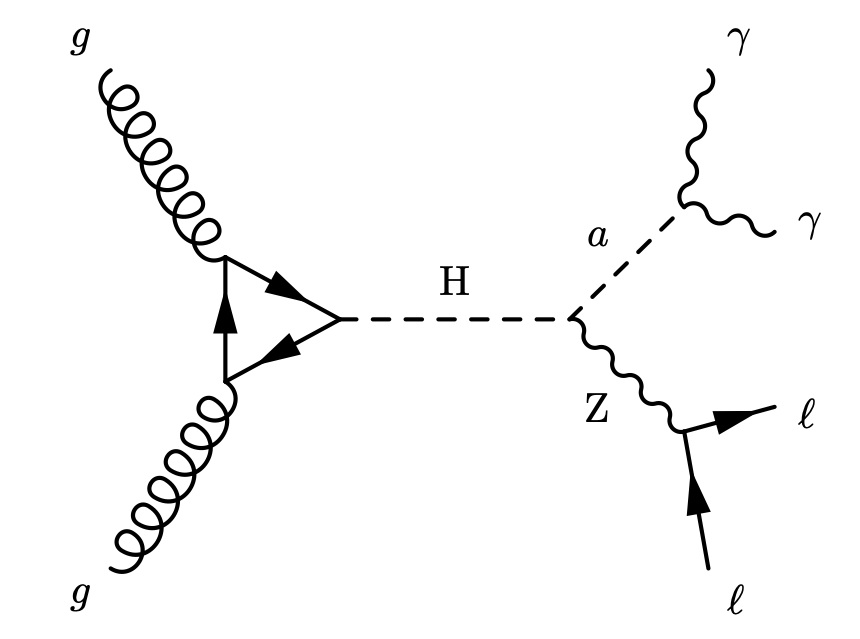
\includegraphics[width=0.45\textwidth]{Thesis (Version 2246)/figures/chapter04/Feyman_diagram.png}
    \bicaption{\quad \centering 希格斯玻色子BSM衰变为一个Z玻色子和一个轻赝标量玻色子,随后分别衰变为两个轻子和两个光子的费曼图}{\quad \centering Feynman diagram for a BSM decay of the H boson into a Z boson and a light pseudoscalar boson, subsequently decaying to two leptons and two photons, respectively}
    \label{fig:Feyman}
\end{center}
\end{figure}

由于我们假设Z玻色子和类轴子都是在壳(On-shell)的粒子,动力学所允许的类轴子质量范围为$m_{a}<m_{H}-m_{Z}\approx35\GeV$,其中,$m_H$和$m_Z$分别为希格斯粒子质量和Z玻色子质量。而对于质量低于1$\GeV$的类轴子,衰变产生的两个光子在探测器中不再能够被区分。因此,本分析只考虑了类轴子的质量范围为$1 < m_{a} < 30\GeV$。

本章结构如下,第\ref{sec:MCData}节介绍了本分析所使用的数据和模拟样本的信息,第\ref{sec:Trigger}节介绍了触发的选择,第\ref{sec:EventReco}节介绍了本分析中所使用的粒子重建,第\ref{sec:EventSelect}节介绍了对信号事例的筛选,第\ref{sec:BDT}节论述了利用参数化的多变量分析的方法提高信号显著度,第\ref{sec:Fit}节介绍了信号提取过程中所使用的统计学方法,第\ref{sec:Bkg}节介绍了本分析中对本底过程的建模,第\ref{sec:Sig}节介绍了对信号过程的建模,第\ref{sec:Sys}节详细介绍了本分析中所涉及的系统误差,最后第\ref{sec:Result}节给出了分析结果。

\section{数据和模拟样本}\label{sec:MCData}

本分析使用了CMS探测器在整个Run2运行期间收集到的质子-质子对撞数据,主要包括探测器于2016年、2017年和2018年间收集的数据,对应的质心能量为13~\si{TeV},三年总的积分亮度为138~\si{fb^{-1}}。本分析所使用的事例模拟和重建都基于CMS合作组开发的软件框架,名为CMSSW。根据探测器运行时期发生的不同情况,对应的分析软件框架会有实时的更新以应对这些变化,因此CMSSW衍生出来了众多版本。本分析所使用的分析框架正是基于CMSSSW\_10\_6\_26,使用的数据版本为Ultra-Legacy,简称UL。

在2016年的探测器运行取数期间,大量硅微条探测器中的高能沉积导致了前端芯片APV25出现短暂的过饱和,使得探测器的读出系统中出现了显著的死时间(Dead-time)。为了解决这个问题,CMS探测器在此后的取数中添加了前向放大器反馈电压偏置(Preamplifier Feedback Voltage Bias,VFP),并对之前收集到的数据进行了修正。因此,在UL版本的数据中,2016年的数据被分为了pre-VFP和post-VFP两部分,其中pre-VFP部分又被称为2016APV。

对于信号样本,本分析利用了MADGRAPH5\_aMC@NLO产生子~\cite{alwall2014automated, Alwall:2007fs, Frederix:2012ps}产生了领头阶的$pp\rightarrow \HZa$信号样本。样本包括CMS实验整个run2三年的数据(2016年、2017年和2018年),针对每年都产生了14个具有不同类轴子质量的信号样本:1到10$\GeV$之间以1$\GeV$为步长,共10个质量点;10到30$\GeV$之间以5$\GeV$为步长,共4个质量点。在模拟中,希格斯粒子的质量被设置为125$\GeV$,并且只考虑了占主导的胶子融合的希格斯产生模式。其他希格斯产生模式对最终结果的贡献仅占1\%,因此可以忽略不计。

本分析中的主要本底过程来自于标准模型Drell-Yan过程产生的一个Z玻色子和喷注,在这个过程中喷注被误判为光子而成为双轻子和双光子末态的本底。为了进一步优化筛选条件,本分析也利用了MADGRAPH5\_aMC@NLO~\cite{alwall2014automated, Alwall:2007fs, Frederix:2012ps}在领头阶对其进行了模拟。由于本分析所涉及的末态属于稀有过程,直接使用MC模拟本底存在非常大的统计误差,因此在最终的信号提取过程中,本底模型通过直接拟合数据的分布得到,MC本底样本仅用于优化筛选条件。

模拟中的部分子分布函数(Parton Distribution Functions,PDFs)使用的是NNPDF3.1~\cite{Ball:2017nwa},部分子的簇射和强子化利用了PYTHIA 8.230产生子~\cite{Sjostrand:2014zea}进行模拟。为了使模拟样本能够和实验数据相符合,我们还需要相应的调节(Tune),对于三年所有的模拟,使用的tune都是CP5~\cite{Khachatryan:2015pea, Sirunyan:2019dfx}。对于CMS探测器的模拟使用的是GEANT4软件\cite{agostinelli2003geant4, 1610988}。附录~\ref{app:data_lists}列出了本分析所使用的所有数据、信号和本底样本。

\section{触发}\label{sec:Trigger}

对于感兴趣的事例,本分析采用了两级触发系统~\cite{Khachatryan:2016bia}。其中,一级触发就是所谓的硬件触发,由CMS探测器中的硬件利用量能器和缪子探测器中的信息,在大约4~\si{\us}的时间间隔内将事例的筛选率由40~\si{\MHz}降低到大约100~\si{\kHz}。二级触发又被称为高级触发,由针对运行速度优化过的事例重建软件所构成,最终可以将事例的筛选率降低到大约1~\si{kHz}。

由于本分析的末态中含有两个由Z玻色子衰变产生的电子或者缪子,因此可以选择单轻子或者双轻子的触发作为本分析的触发。附录~\ref{app:trigger_lists}列出了本分析所使用的所有触发列表。对于单轻子触发,要求电子的最低横动量为25$\GeV$,缪子的最低横动量为20$\GeV$;对于双电子触发,要求两个电子的最低横动量分别为12$\GeV$和14$\GeV$;对于双缪子触发,要求两个缪子的最低横动量分别为8$\GeV$和17$\GeV$;对于一个电子和一个缪子的触发,要求电子的最低横动量为17$\GeV$,缪子的最低横动量为8$\GeV$。

\section{物理对象的筛选以及效率测量}\label{sec:EventReco}

由于对撞中堆积事例的存在,使得每次对撞都会产生许多对撞顶点。在本分析中,事例的初级对撞顶点选为硬散射程度最高的顶点。此外,由于衰变末态中存在两个电子或者缪子以及两个光子,因此对电子、缪子和光子的重建筛选对本分析具有重要的意义。

\subsection{电子筛选}

对电子的重建在第~\ref{subsec:EGReco}节已经有过介绍,电子候选者通过对径迹和簇射的对应观测量进行宽松筛选(Loose cut)得到,目的是为了能够尽可能高的保留电子的事例率,同时也可以排除掉一部分QCD本底。在本分析中,我们对宽松的电子(Loose electron)定义为:电子的横向动量$\mathrm{p_{T}^{e}}>7\GeV$,重建范围为$|\eta^{e}|<2.5$,并且满足宽松的初级顶点限制(重建顶点在横向平面的位移$d_{xy}<0.5~\si{\cm}$、重建顶点在束流方向的位移$d_{z}<1~\si{\cm}$)。

在筛选出loose电子后,为了进一步筛选出纯度更高的电子,本分析采取了多变量分析的辨别方法。对电子的辨别由运行在梯度提升(Gradient Boosting)框架上的机器学习算法来实现,这个算法利用了一些来自电磁量能器、簇射和电子轨迹之间的匹配度、径迹测量以及粒子流隔离度求和等信息作为输入变量对模型进行训练,同时梯度提升框架也保证了训练出来的模型具有非常好的泛化能力。而后将训练结果应用于数据,进而筛选出纯度更高的电子。本分析所使用的训练模型由CMS实验$H\rightarrow ZZ\rightarrow 4\ell$物理分析组~\cite{cmsHZZ}提供,表格~\ref{tab:ele_ID_input_variables}列出了训练模型所使用的输入变量。利用各个电子的这些变量作为模型的输入,可以得到与之对应的输出分数(Output score),然后再对output score进行阈值筛选进而可以得到纯度更高的电子。表格~\ref{tab:ele_ID_WP}列出了不同年份、不同横动量范围和不同$\eta$范围的电子提升决策树输出分数阈值,所有提升决策树输出分数大于这些阈值的电子被保留下来,并称这些电子为严格的电子(Tight electron)。


\begin{table}[h!]
\scriptsize
    \centering
    \bicaption{\quad \centering 电子识别分类器的输入变量概述}{\quad \centering Overview of input variables to the electron identification classifier}
    \resizebox{\textwidth}{!}{
    \begin{tabular}{cl}

\hline %----------------------------------------------------------------------------------------
%\multicolumn{4}{|c|}{Datasets}                                                                \\
观测量类型    &  观测量名称      	\\
\hline %----------------------------------------------------------------------------------------

\multirow{6}{*}{簇射形状变量}
	&  沿$\eta$和$\varphi$方向的能量晶体数谱的标准差:$\sigma_{i\eta i\eta}$,$\sigma_{i\varphi i\varphi}$		\\
	&  超级簇射在$\eta$和$\phi$方向的宽度		\\
	&  位于电子超级簇射之后的强子量能器所沉积的能量和超级簇射能量的比值:$H/E$			\\
	&  环状变量:$(E_{5\times5} - E_{5\times1})/E_{5\times5}$			\\
	&  超级簇射中种子和相邻晶体能量的总和:$R_{9}$			\\
	&  对于端盖部分电子的训练,预簇射中的沉积能量所占总能量的比例:$E_{PS}/E_{raw}$			\\
\hline
\multirow{2}{*}{径迹--簇射匹配度变量}
	& 能量--动量匹配度:$E_{tot}/p_{in}$, $E_{ele}/p_{out}$,$1/E_{tot} - 1/p_{in}$ 			\\
	& 位置匹配度:$\Delta\eta_{in}$, $\Delta\varphi_{in}$,$\Delta\eta_{seed}$			\\
\hline
\multirow{5}{*}{径迹变量}
        & 动量损失百分比:$f_{brem} = 1 - p_{out}/p_{in}$	\\
        & 由KM方法所求得的径迹和GSF径迹的击中数:$N_{KF}$,$N_{GSF}$   \\
        & KM径迹和GSF径迹的简化$\chi^2$值:$\chi^{2}_{KF}$,$\chi^{2}_{\textrm{GSF}}$ \\
        & 预期存在但缺失的内部击中数 \\
        & 转换顶点拟合的概率变换:$\chi^2$   \\
\hline
\multirow{3}{*}{隔离度变量}
& 粒子流光子隔离度   \\
& 粒子流带电强子隔离度   \\
& 粒子流中性强子隔离度   \\
\hline
\multirow{1}{*}{与堆积事例相关的变量}
& 事例中的平均能量密度: $\rho$ \\
\hline %----------------------------------------------------------------------------------------
     \end{tabular}
     }
\small
    \label{tab:ele_ID_input_variables}
\end{table}




\begin{table}[h!]
%\scriptsize
    \centering
    \bicaption{\quad \centering 通过电子辨别所需的最低提升决策树分数}{\quad \centering Minimum BDTs score required for passing the electron identification}
    \begin{tabular}{ccc c c}
\hline

\hline %----------------------------------------------------------------------------------------
\multicolumn{2}{c}{minimum BDTs score}    &  $|\eta| < 0.8 $ & $0.8 < |\eta| < 1.479$ 	& $|\eta| > 1.479$      \\
\hline %----------------------------------------------------------------------------------------
2016 Datasets & $ 5 < \pt < 10 $ GeV &  1.894      & 1.807  	& 1.647		\\
& $\pt > 10$ GeV         &  0.339	& 0.252		&  -0.686	\\
\hline %------------------------------------------------------------------
2017 Datasets & $ 5 < \pt < 10 $ GeV &  1.544    & 1.502  	& 1.773		\\
& $\pt > 10$ GeV         &  0.157    & 0.0274	& -0.623	\\
\hline %------------------------------------------------------------------
2018 Datasets & $ 5 < \pt < 10 $ GeV &  0.9044    & 0.9094  	& 0.9444		\\
& $\pt > 10$ GeV         &  0.1969    & 0.0759	& -0.5169	\\
\hline %------------------------------------------------------------------
     \end{tabular}
\small
    \label{tab:ele_ID_WP}
\end{table}

在低动量区域($5<\pt<10\GeV$),电子的tight筛选对真电子的选择效率平均可以达到80\%,同时可以拒绝大约95\%的假电子;而在高动量区域($\pt>10\GeV$),对真电子的选择效率可以达到大约97\%,同时拒绝大约92\%的假电子。

此外,为了确保重建出来的轻子和我们选择的对撞顶点相符合,我们还要求这两者具有一个相互关联的轨迹,这个轨迹相对于事例的初级对撞顶点具有较小的对撞参数。为了实现这一要求,可以定义变量$\mathrm{SIP_{3D} = IP/\sigma_{IP}}$,其中IP指的是距离初级对撞顶点最近的轻子三维对撞参数,$\mathrm{\sigma_{IP}}$指的是对应的不确定性。在本分析中,我们要求所有的电子满足$\mathrm{|SIP_{3D}|<4}$。

\subsection{缪子筛选}

第~\ref{subsec:MuonReco}节对缪子的重建进行了介绍。在本分析中,缪子的选择首先来自于重建出来的全局缪子或者径迹室缪子。而后宽松的缪子(Loose muon)被定义为横动量$\pt>5\GeV$、$|\eta|<2.4$、对撞参数$d_{xy}<0.5~\si{cm}$和$d_{z}<1~\si{cm}$。

对于横动量$\pt<200\GeV$的loose muon,如果它能够通过粒子流缪子辨别(PF muon ID)就称为被辨别的缪子(Identified muon);而对于横动量$\pt>200\GeV$的loose muon,如果它们能够通过PF muon ID或者径迹室高横动量辨别(Tracker High-$\pt$ ID),也称为identified muon。PF muon ID由CMS实验官方提供,工作点选为loose ID;Tracker High-$\pt$ ID也由CMS实验官方提供,工作点仍选为loose ID,定义如表格~\ref{tab:highPtID}所示。利用宽松的辨别条件筛选缪子的目的是希望能够尽可能多的保留缪子事例,因为在CMS探测器中,缪子的重建具有非常干净的本底,尽可能多的保留缪子事例可以提高信号显著度。

\begin{table}[h]
    \begin{small}
    \begin{center}
    \bicaption{\quad \centering 缪子通过径迹室高横动量辨别所需的要求}{
      \quad \centering The requirements for a muon to pass the Tracker High-$\pt$ ID}
    \begin{tabular}{ll}
      \hline
      字面描述         & 定义                 \\
      \hline
      缪子station匹配度          & 缪子至少与两个缪子station中的片段相匹配 \\
      \hline                                                          
      好的$\pt$测量         & $\frac{\pt}{\sigma_{\pt}} < 0.3$      \\
      \hline
      xy平面上的顶点兼容性   & $d_{xy} < 2$~mm                       \\
      \hline
      z方向上的顶点兼容性     & $d_{z} < 5$~mm                        \\
      \hline
      像素探测器击中          & 至少存在一个像素击中           \\
      \hline
      径迹室击中       & 击中至少在6层径迹室探测器中出现  \\
      \hline
    \end{tabular}
    \label{tab:highPtID}
    \end{center}
    \end{small}
\end{table}

此外,一个单独的缪子可能被错误的重建为两个或者更多的缪子。针对这一情况,可以利用以下的“ghost-cleaning”这一步骤进行处理:
\begin{itemize}
    \item 要求缪子是不属于global muons的tracker muons。
    \item 如果重建出来的两个缪子具有超过50\%的重叠部分,则去除重建质量比较差的缪子。
\end{itemize}

为了降低在簇射中的强子衰变所产生的轻子对缪子辨别的影响,本分析利用了轻子的相对隔离度这一变量,定义如下:

\begin{equation}\label{eq:4-01}
    I^{\ell} = \left(\sum \pt^{\text{charged}}+\max[0,\sum \pt^{\text{neutral}}+\sum \pt^{\gamma}-\pt^{\text{PU}}]\right)/\pt^{\ell}
\end{equation}
其中,求和遍历所有位于半径$\dR<0.3$的锥形体内的PF候选体;$\pt^{i}$表示单独的带电强子、中性强子、光子或者来自于堆积事例的粒子的横向动量。在本分析中,缪子相对隔离度的工作点同样由CMS实验$H\rightarrow ZZ\rightarrow 4\ell$物理分析组~\cite{cmsHZZ}提供,要求$\mathrm{I^{\ell}<0.35}$。我们将同时通过以上选择条件的缪子称为严格的缪子(Tight muon)。此外,与电子一样,本分析同样要求缪子的$\mathrm{|SIP_{3D}|<4}$。

\subsection{末态辐射光子的筛选}

当电子或者缪子穿过探测器时,会和探测器中的物质发生相互作用,发生韧致辐射。此时,末态的轻子会辐射出一个光子,称为末态辐射光子(Final State Irradiation Photon, FSR Photon)。本分析利用了末态辐射光子恢复算法,可以将辐射出去的光子添加回轻子中,进而可以有效的提高双轻子的不变质量谱分辨率。该算法首先从PF光子对象中选择候选体,具体筛选过程如下:
\begin{enumerate}
    \item 对PF光子的预选则包括:要求光子的横动量$\mathrm{p_{T,\gamma}}>2\GeV$,赝快度$|\eta|<2.4$以及相对PF隔离度小于1.8。光子的相对PF隔离度和轻子的相对隔离度计算方法类似,所有的PF粒子要求位于光子半径R为0.3的锥体内,带电强子要求横动量大于0.2$\GeV$并且位于光子候选体半径R为0.0001的锥体外,中性强子和光子的横动量要求大于0.5$\GeV$并且位于光子候选体半径R为0.01的锥体外,来自堆积事例的贡献项和轻子的相对隔离度所要求的半径和横动量阈值相同。
    \item 超级簇射否决(Supercluster veto):移除和任何通过loose ID和SIP筛选的电子相匹配的PF光子。匹配度是通过直接计算两个PF候选体之间的$\dR$来得到的。
    \item 在所有通过loose ID和SIP筛选的轻子事例中,与轻子距离最近的光子被选为对应轻子的FSR光子。
    \item 如果被选出的光子不满足$\mathrm{\dR(\gamma, l) / E_{T, \gamma}^{2}<0.012}$以及$\mathrm{\dR(\gamma, l)<0.5}$,则丢弃这个光子候选体。
    \item 如果对应的轻子有多个FSR光子候选体,选择$\mathrm{\dR(\gamma, l) / E_{T, \gamma}^{2}}$最小的光子。
    \item 对于所有通过loose ID和SIP筛选的轻子,在计算相对隔离度时将筛选出来的FSR光子从求和中剔除掉。
\end{enumerate}


\subsection{光子筛选}

对光子的重建在第~\ref{subsec:EGReco}节已经有过介绍,光子可以利用电磁量能器中的簇射信息进行重建。假光子的来源主要是喷注中的中性介子成分,比如$\pi^{0}$或者$\eta$。这些中性粒子在探测器中迅速的衰变为两个光子,并且由于喷注中的中性粒子具有非常高的横动量,使得衰变产生的两个光子几乎在一条直线上,很难在电磁量能器中将其与单光子事例区分开来。但是由于喷注中含有众多的其他成分,使得在电磁量能器中重建出来的光子候选体周围会有许多其他粒子沉积能量,相比于单光子事例,来自于喷注中的假光子会具有更高的isolation值。因此,可以利用光子的簇射信息对这一部分假光子进行区分。在本分析中,对于横动量$10<\pt<14\GeV$的光子候选体,如果$H/E<0.15$并且$I_{ch}<10\GeV$,就将其定义为宽松的光子(Loose photon);而对于横动量$\pt>14\GeV$的光子候选体,如果$H/E<0.15$,就将其定义为loose photon。

为了进一步区分假光子,本分析使用了CMS实验官方提供的tight cut-based ID。在这个ID中,光子的$\sigma_{i\eta i\eta}$、$H/E$和isolation等变量被用于辨别真假光子,具体定义见表格~\ref{tab:tightPhotonID}。

\begin{table}[h]
    \begin{small}
    \begin{center}
    \bicaption{\quad \centering 桶部和端盖区域的光子tight cut-based ID工作点筛选要求}{\quad \centering Cut-based photon identification requirements for the tight working point in the barrel and end-cap}
    \begin{tabular}{ccc}
      \hline
      Variables         & $|\eta|<1.4$  & $1.4<|\eta|<2.5$               \\
      \hline
      $H/E$          & $<0.021$ & $<0.032$           \\
      $\sigma_{i\eta i\eta}$         & $<0.0099$ & $<0.027$      \\
      $I_{ch}$   & $<0.65\GeV$  & $<0.52\GeV$                     \\
      $I_{n}$     & $<0.32\GeV+0.015E_{T}+$  & $<2.72\GeV+0.012E_{T}+$      \\
              & $2.26\num{2.26e-5}E_{T}^{2}/\mathrm{GeV}$ & $2.26\num{2.3e-5}E_{T}^{2}/\mathrm{GeV}$ \\
      $I_{\gamma}$  & $<2.04\GeV+0.0040E_{T}$ & $<3.03\GeV+0.0037E_{T}$             \\
      \hline
    \end{tabular}
    \label{tab:tightPhotonID}
    \end{center}
    \end{small}
\end{table}

\begin{figure}[htbp]
  \begin{center}
		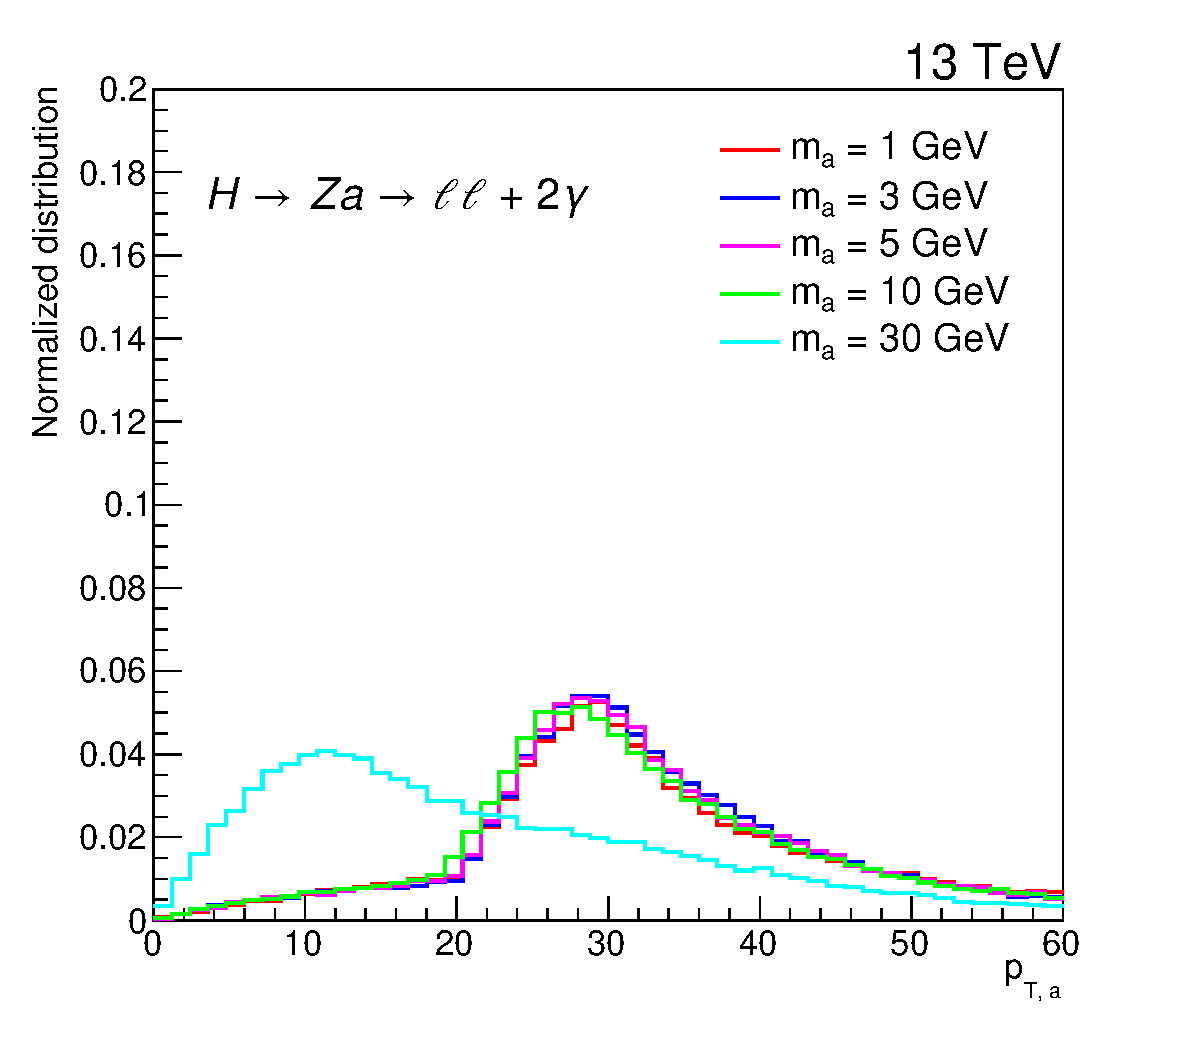
\includegraphics[width=0.45\textwidth]{Thesis (Version 2246)/figures/chapter04/ALP_pt.pdf}    
    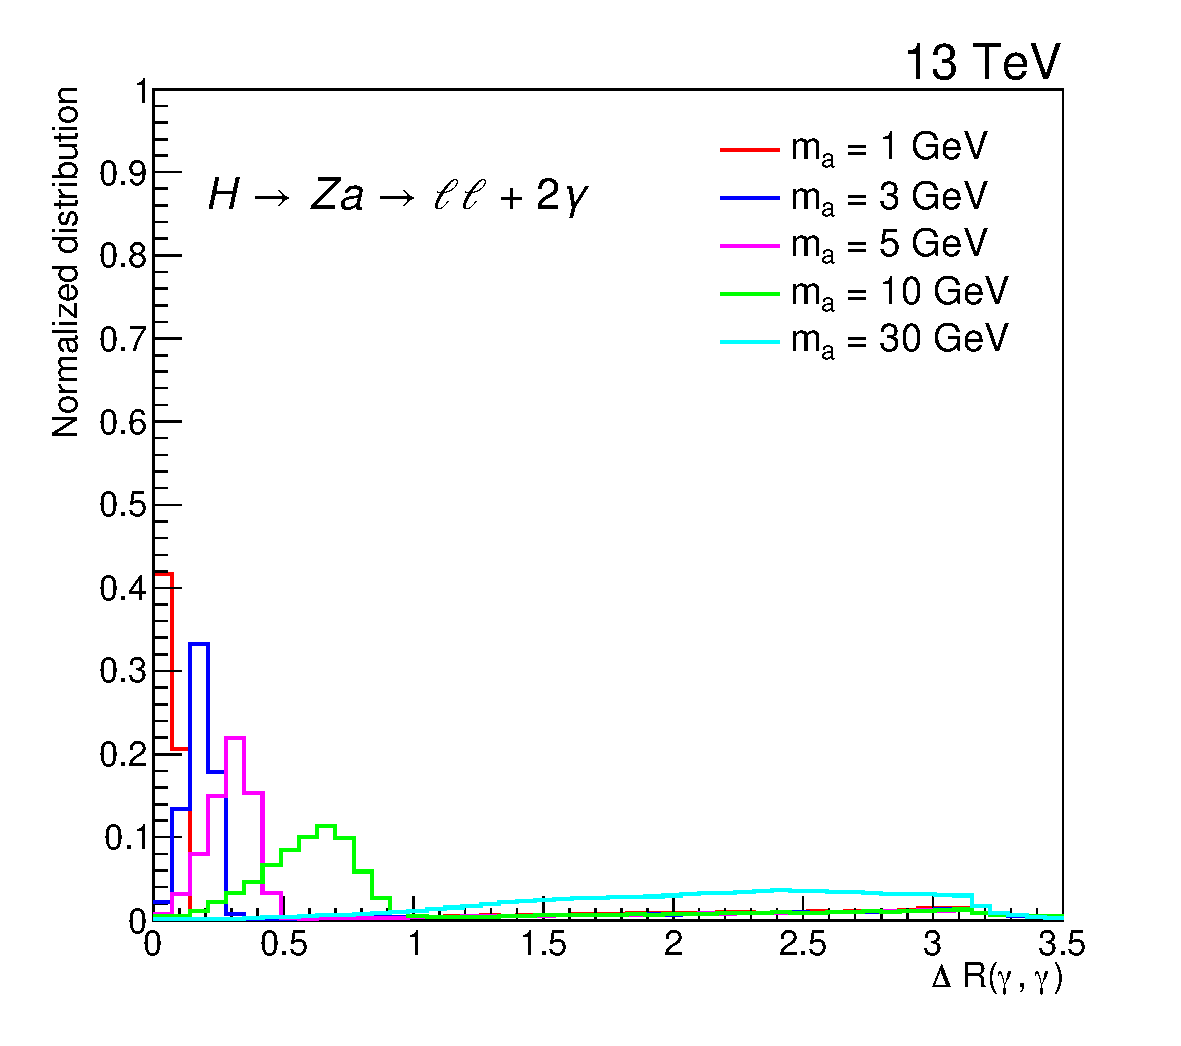
\includegraphics[width=0.45\textwidth]{Thesis (Version 2246)/figures/chapter04/dR_gg.pdf} \\
    \bicaption{\quad \centering 左图:不同ALPs质量点重建出的ALPs的横动量分布。右图:不同ALPs质量点的$\dR(\gamma,\gamma)$分布。所有的分布都被归一化}{\quad \centering Left: Reconstructed ALPs $\pt$ distributions for different ALPs mass points. Right: $\dR(\gamma,\gamma)$ distributions for different ALPs mass points. All of these distributions have been normalized}
    \label{fig:dR_pt}
\end{center}
\end{figure}

但是,当类轴子的质量比较小的时候,由Higgs衰变产生的类轴子会具有比较高的横动量,此时由类轴子衰变产生的两个光子会具有非常小的角距离,具体表现为两个光子之间的$\dR$会非常小。图~\ref{fig:dR_pt}展示了不同类轴子质量下重建出的类轴子$\pt$和由类轴子衰变产生的两个光子之间的$\dR$分布。可以发现,质量越低的类轴子倾向于具有更高的横动量,由此衰变产生的两个光子具有更小的$\dR$。对于质量小于5$\GeV$的类轴子来说,衰变产生的两个光子的$\dR<0.3$,而用于辨别真假光子的tight cut-based ID中使用了光子隔离度变量$I_{\gamma}$,这个变量的计算利用了光子周围半径$\dR=0.3$的锥形体内的所有PF光子,这就意味着质量小于5$\GeV$的类轴子衰变产生的两个光子会在半径$\dR=0.3$的锥形体内部分重叠,使得计算出来的光子隔离度偏大进而将信号事例辨别为本底事例;除此之外,相距很近的两个光子也会对$\sigma_{i\eta i\eta}$的计算产生影响,使得信号事例的$\sigma_{i\eta i\eta}$结果偏大而将信号事例辨别为本底事例。图~\ref{fig:sigma_Iso}展示了不同ALPs质量点衰变产生的光子在桶部和端盖区域的$I_{\gamma}$和$\sigma_{i\eta i\eta}$分布。考虑到以上原因,为了在低质量区域内保留足够的信号选择效率,我们最终决定使用新设计的光子辨别ID,去除对信号选择效率影响比较大的$I_{\gamma}$和$\sigma_{i\eta i\eta}$作为本分析的光子辨别ID。图~\ref{fig:IDCorr_eff}展示了对于不同类轴子质量点官方cut-based photon ID和新设计的光子辨别ID之间的信号效率对比图,可以发现去除$I_{\gamma}$和$\sigma_{i\eta i\eta}$这两个变量可以在类轴子的低质量区域内将信号的选择效率恢复到和高质量区域相同的水平。但是,去除这两个变量的同时会导致本底假光子事例的增加。为此,本分析采取了参数化的决策树法(Parameterized BDTs),将$I_{\gamma}$和$\sigma_{i\eta i\eta}$这两个变量连同其他动力学变量一起作为BDTs的输入进而进一步的对本底事例进行区分,详细步骤会在第~\ref{sec:BDT}节进行介绍。

\begin{figure}[htbp]
  \begin{center}
	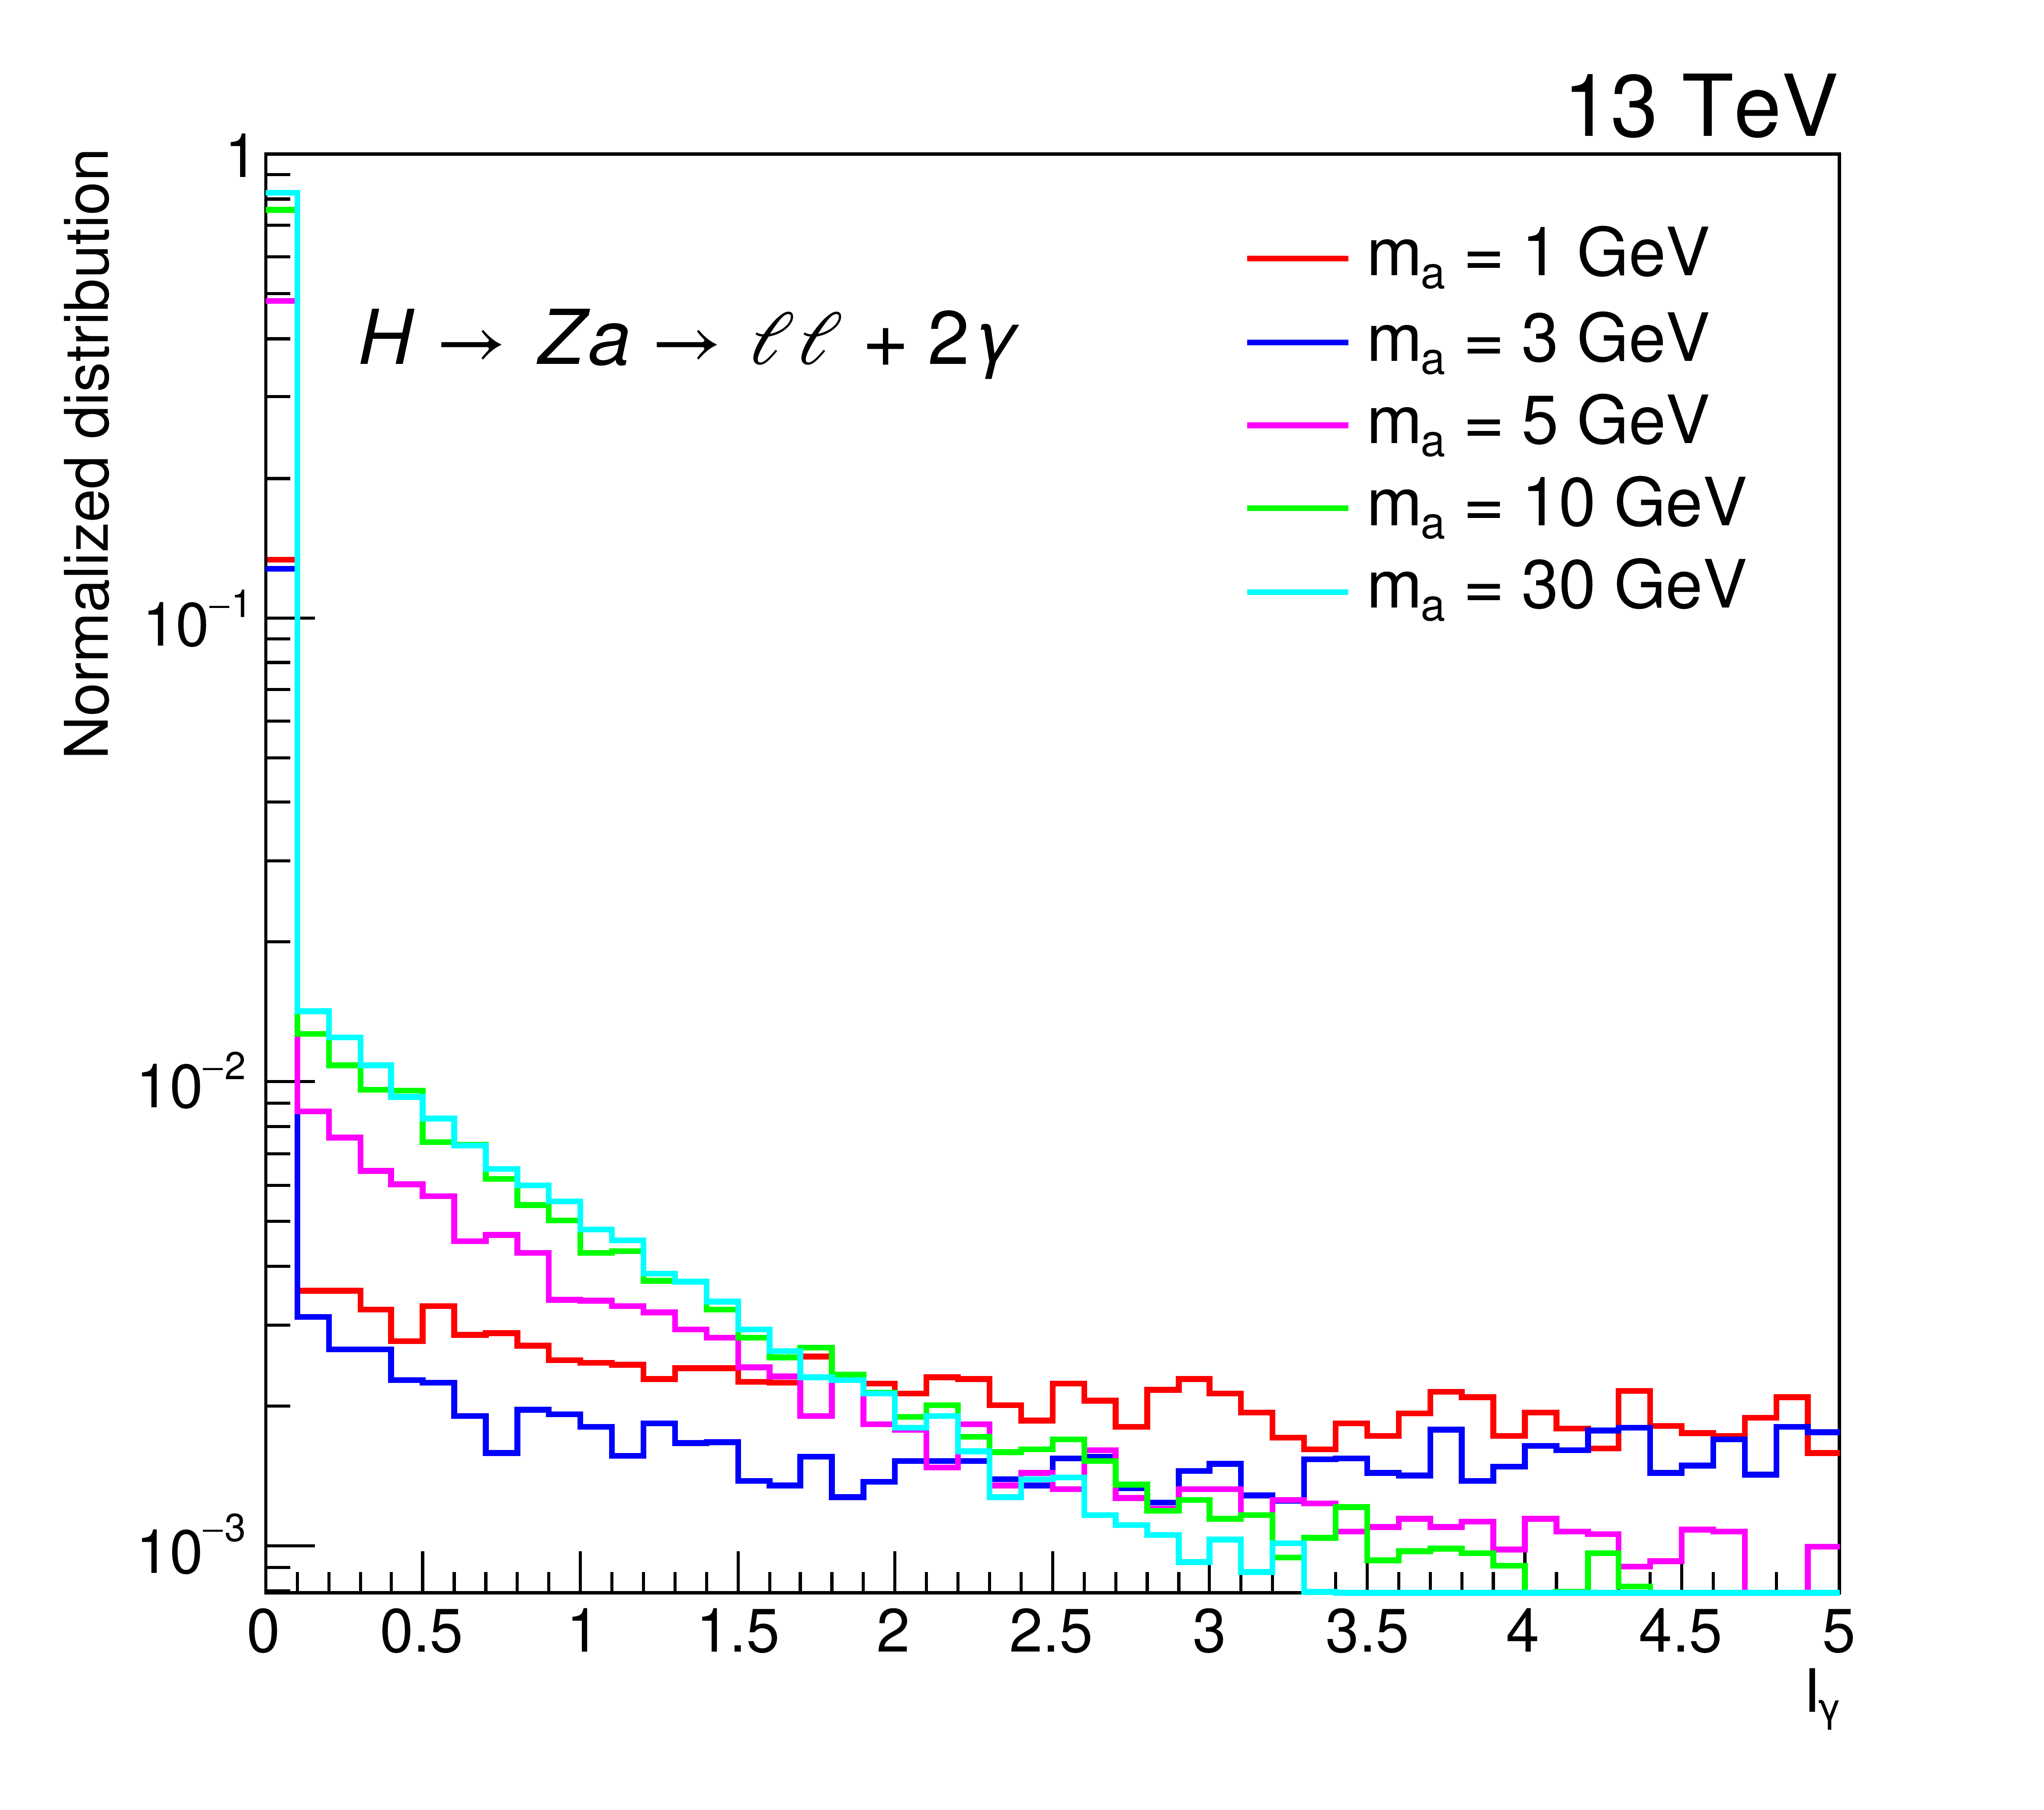
\includegraphics[width=0.45\textwidth]{figures/chapter04/pho_phoIso_EB.png}
    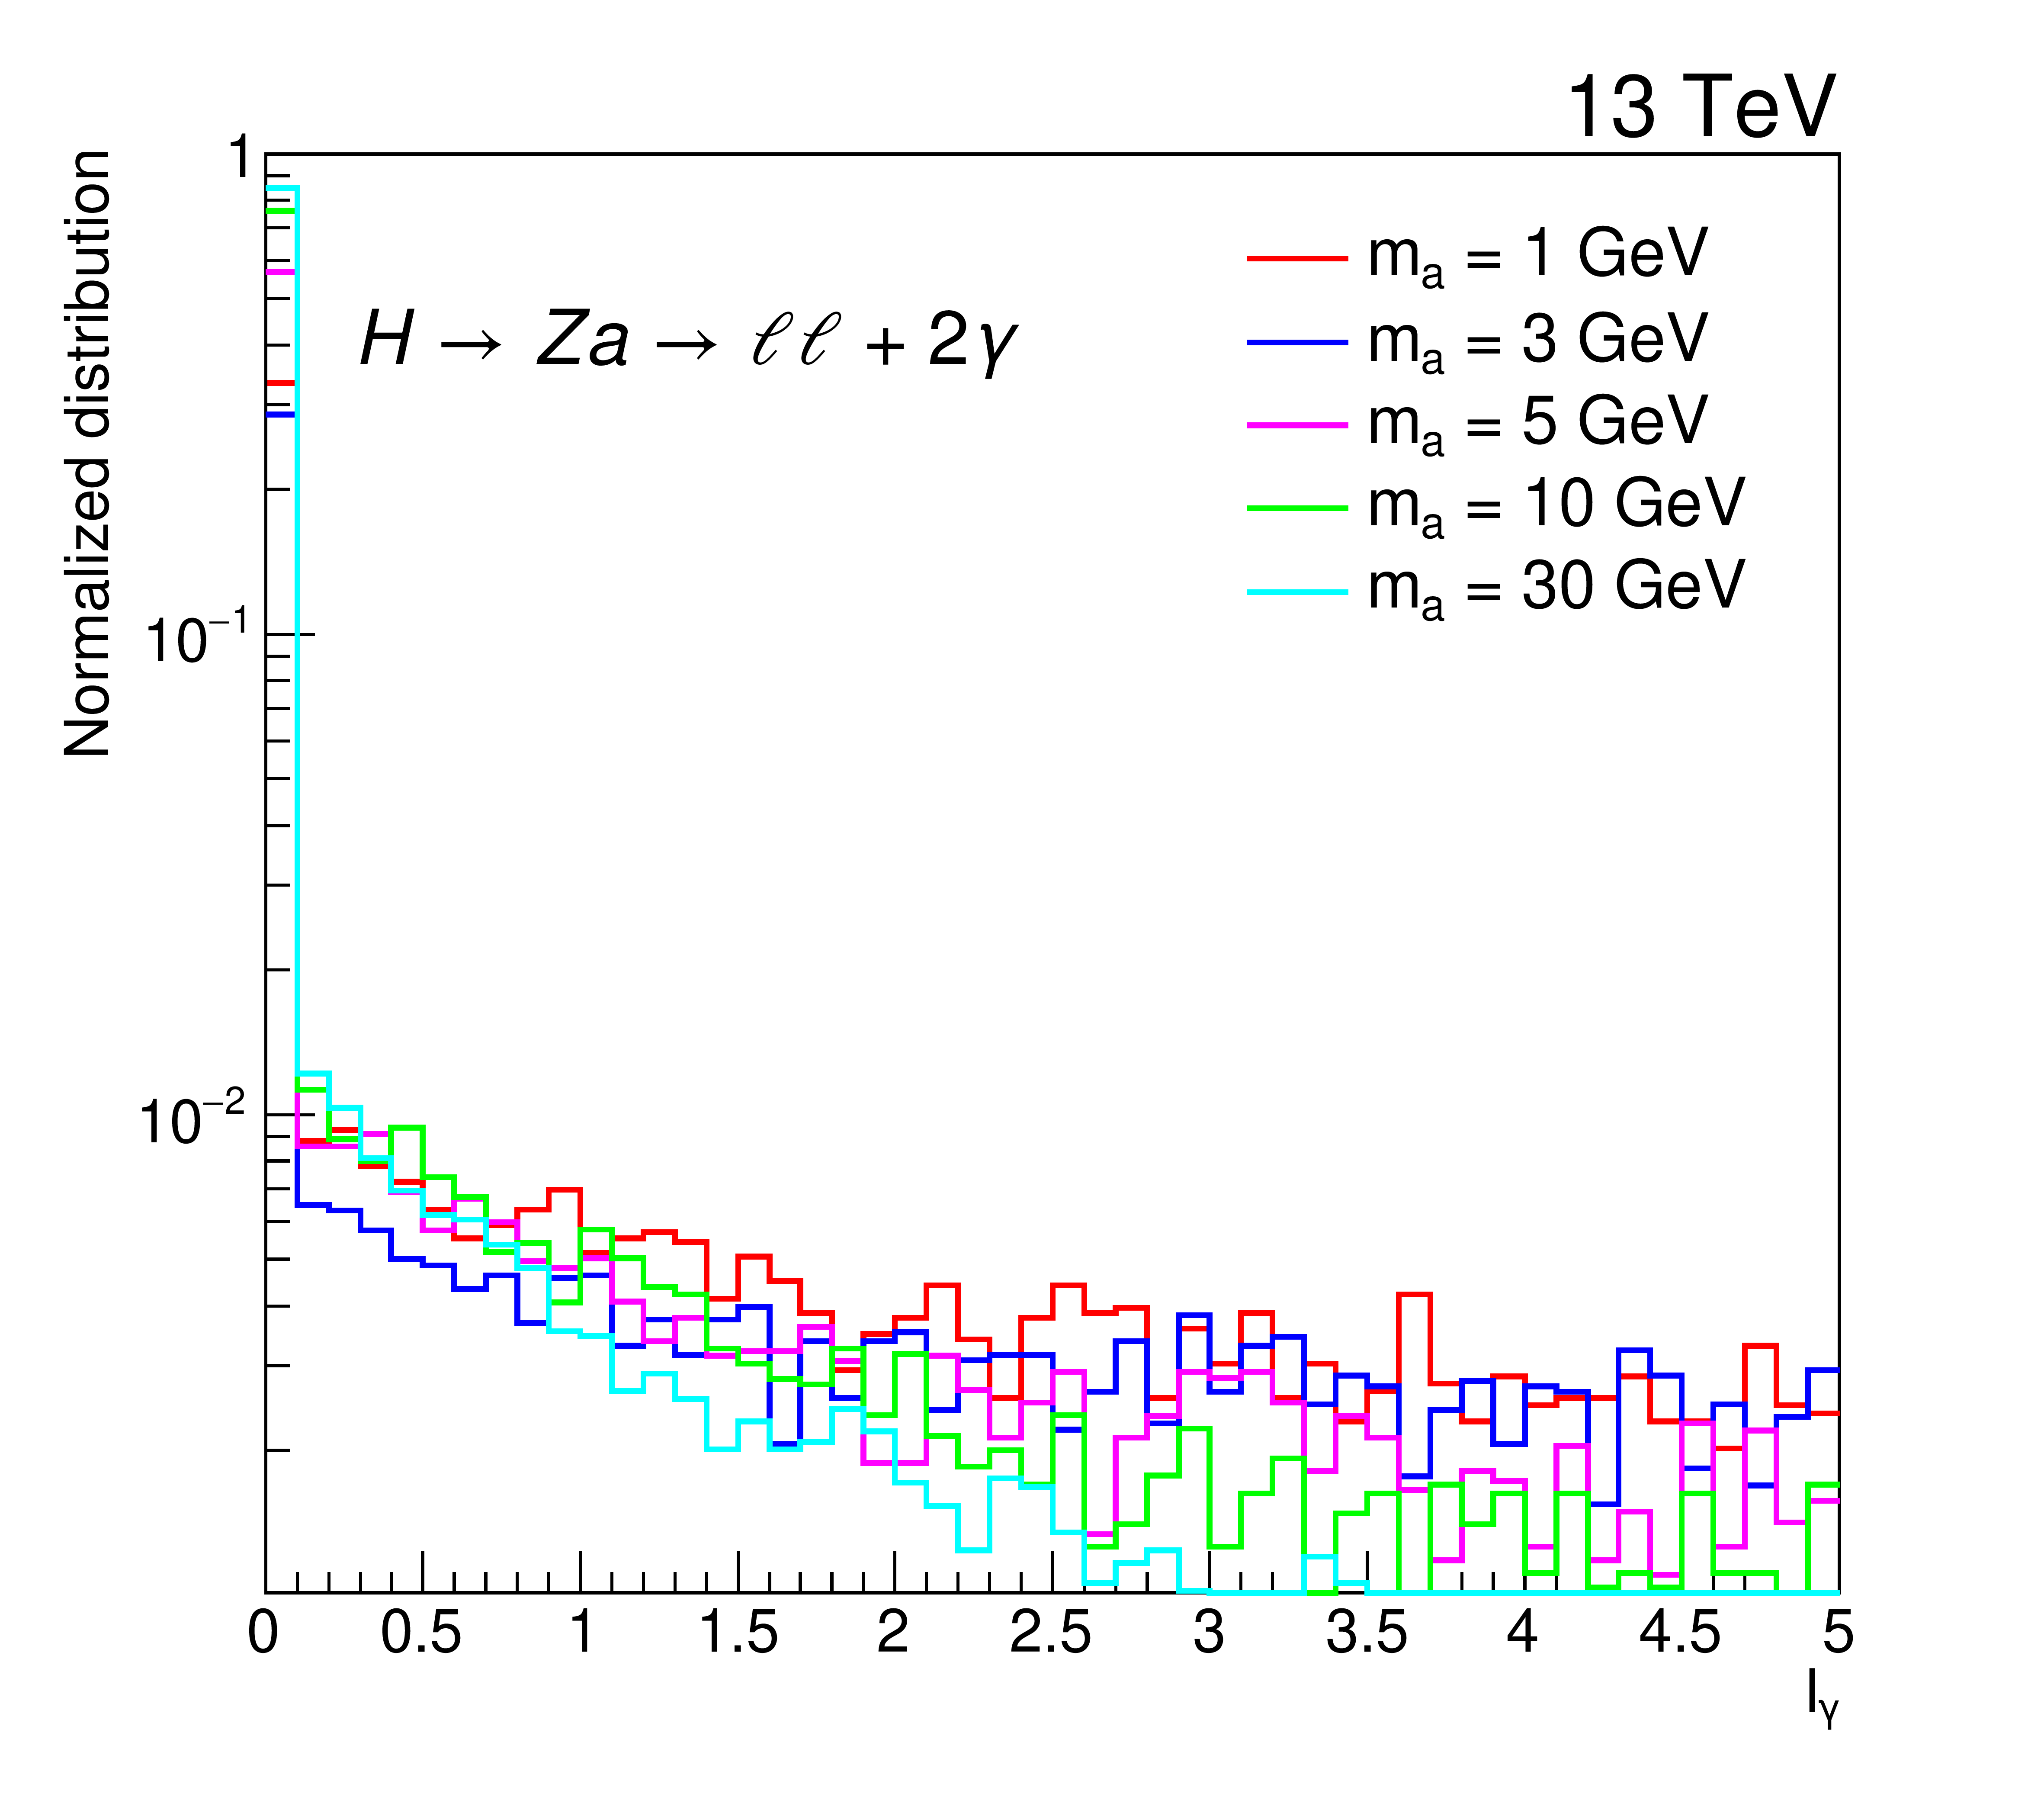
\includegraphics[width=0.45\textwidth]{figures/chapter04/pho_phoIso_EE.png} \\
    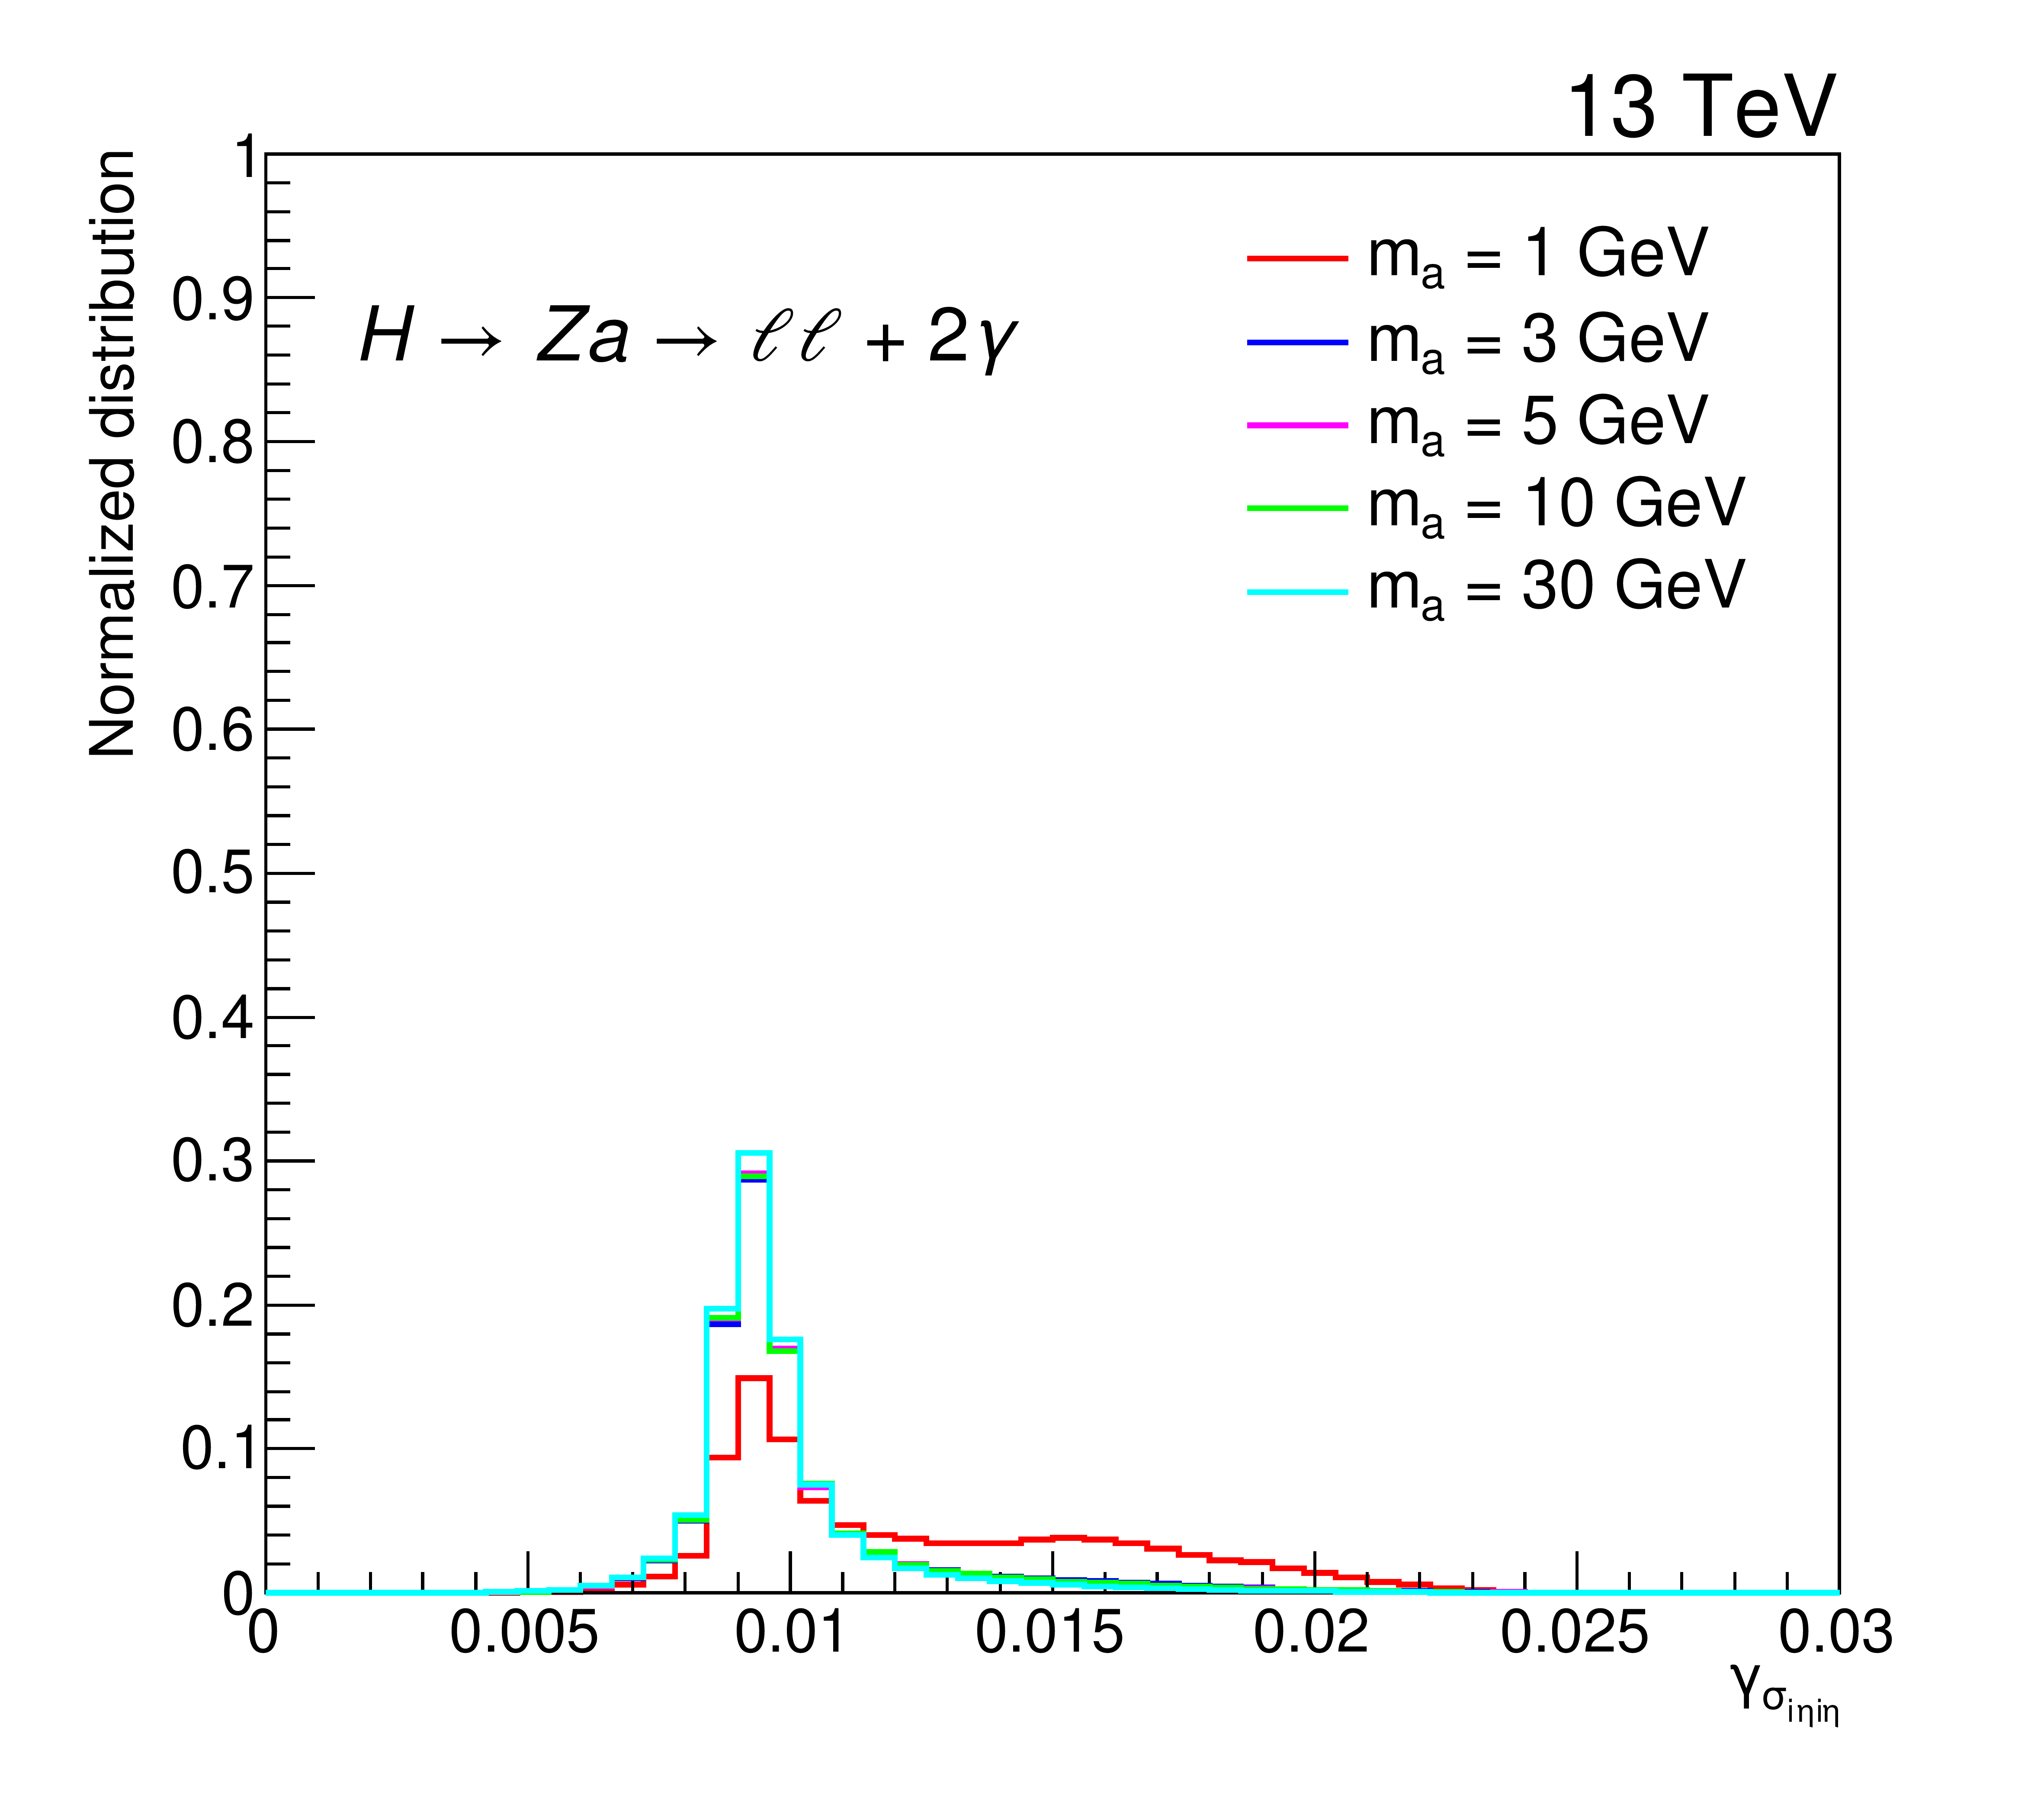
\includegraphics[width=0.45\textwidth]{figures/chapter04/pho_sigmaIetaIeta_EB.png}
    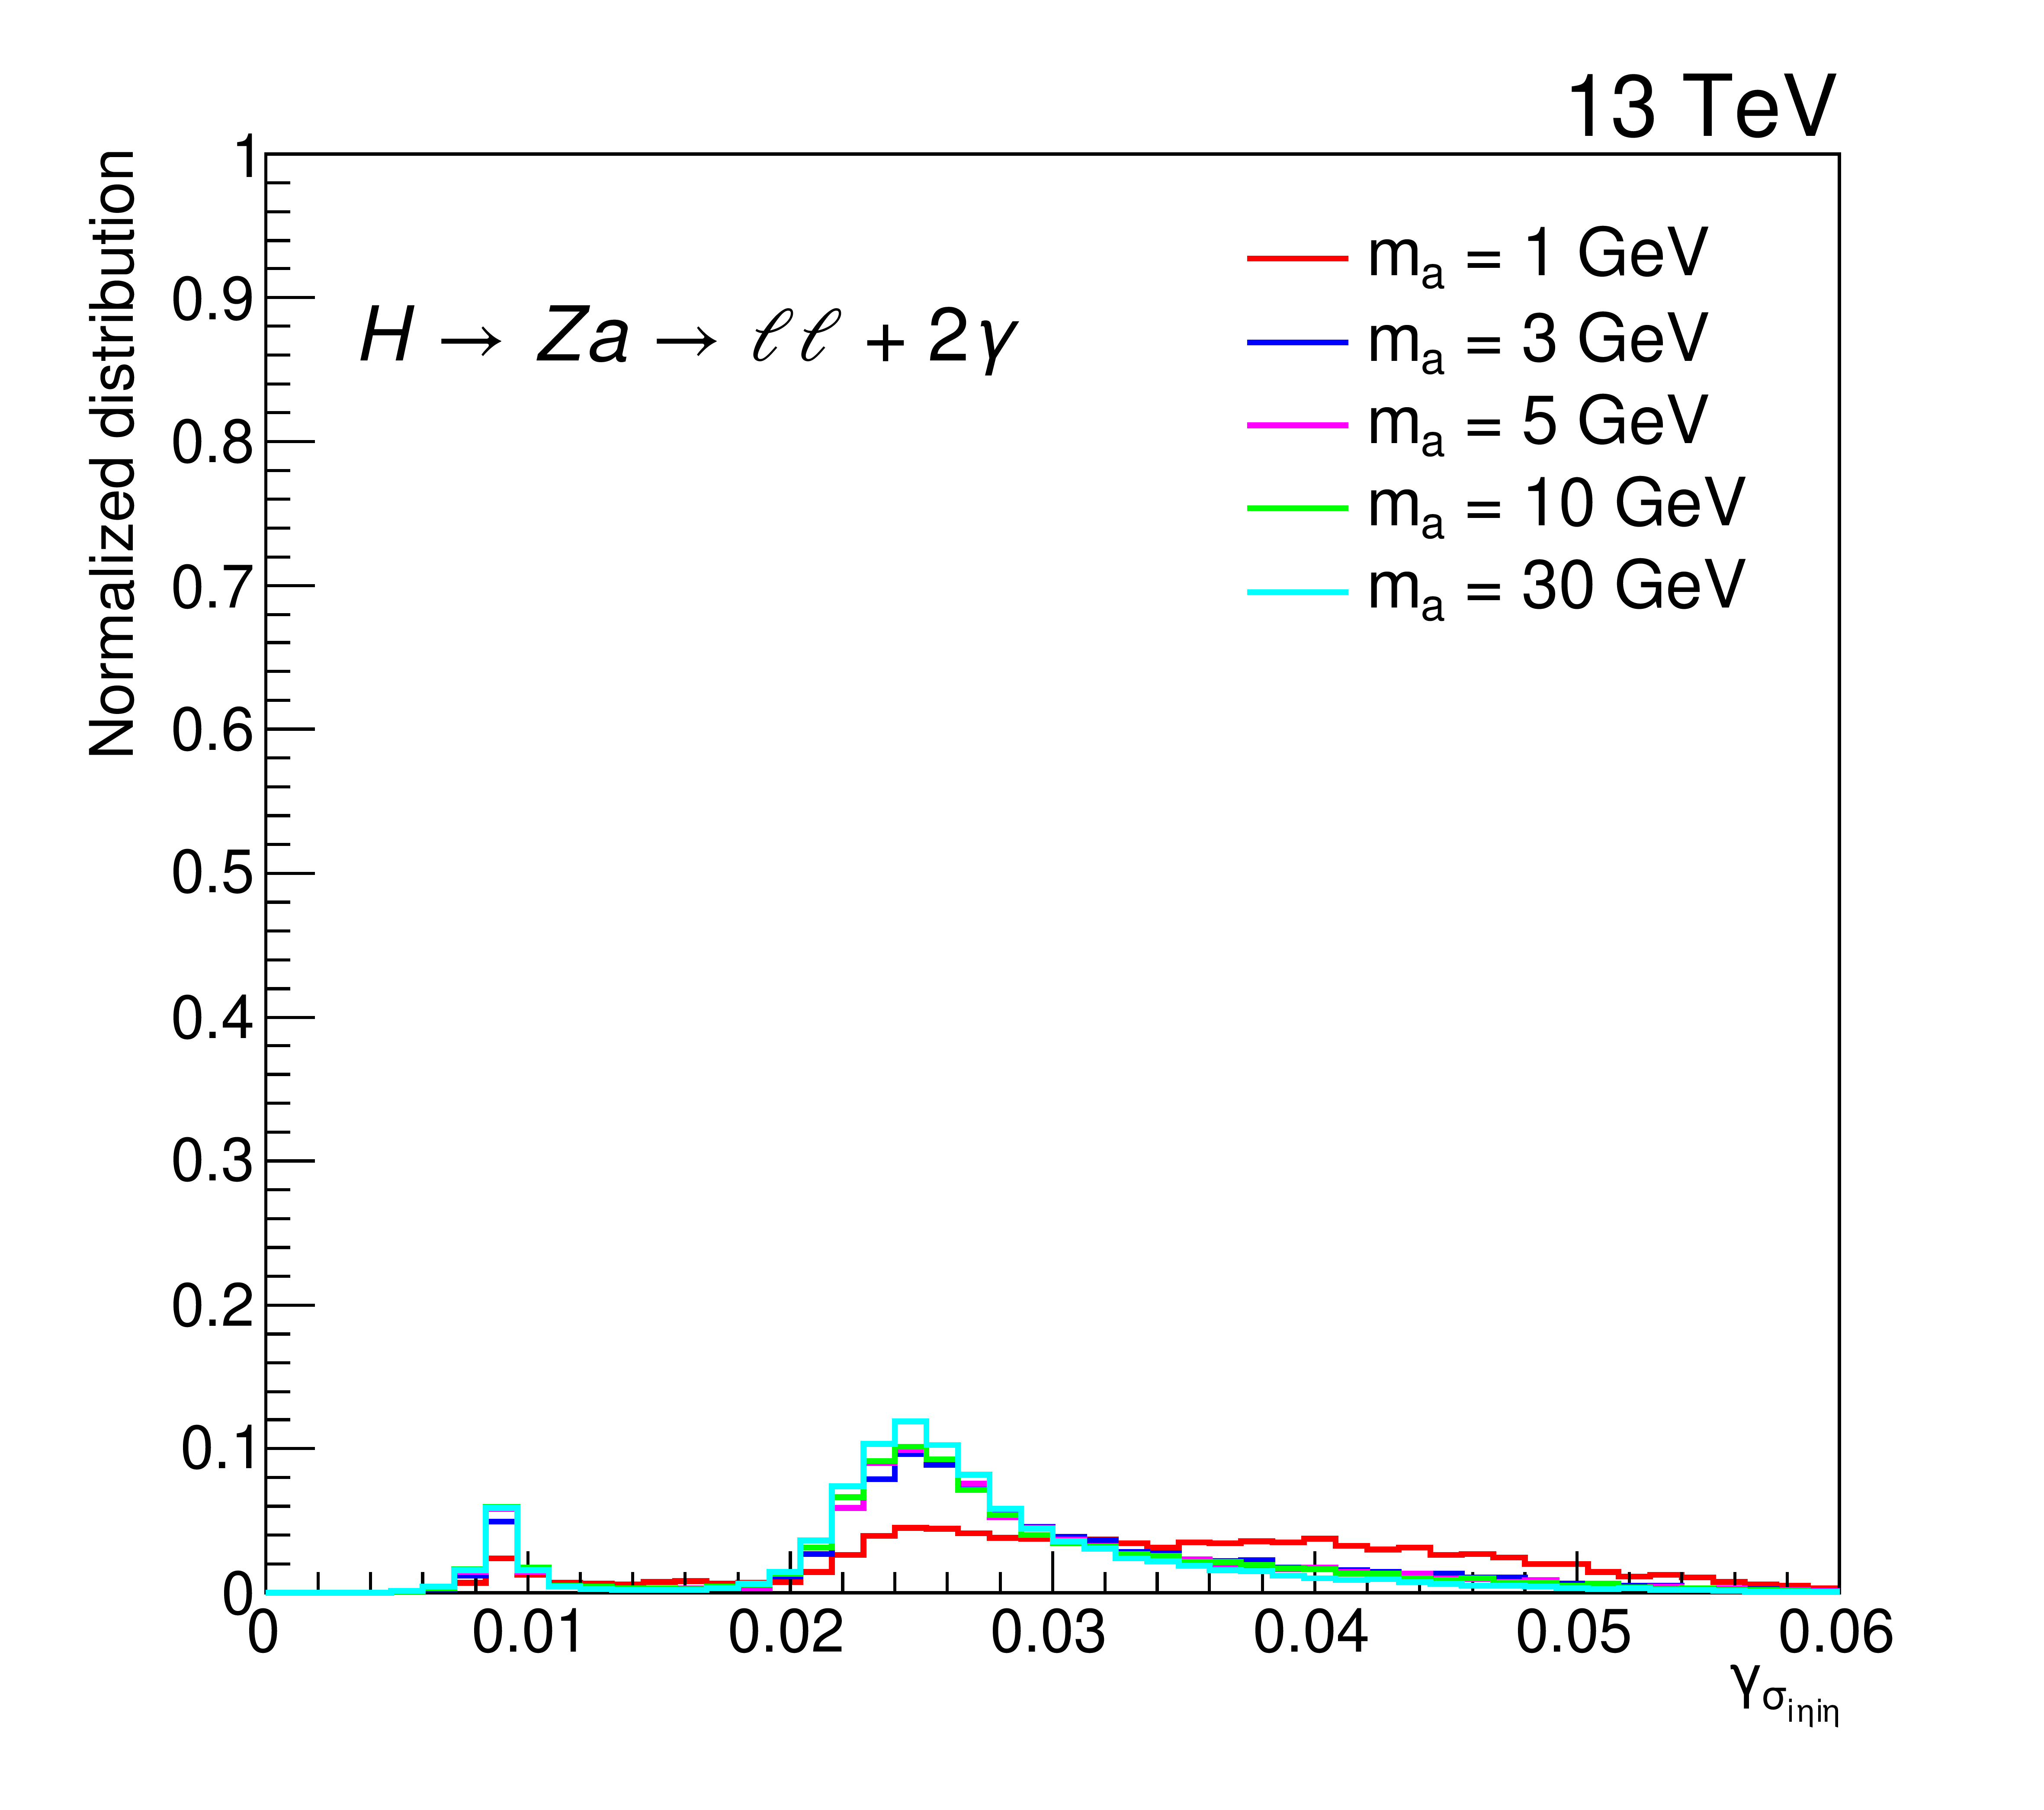
\includegraphics[width=0.45\textwidth]{figures/chapter04/pho_sigmaIetaIeta_EE.png} \\
    \bicaption{\quad \centering 上图:不同ALPs质量点的PF光子隔离度分布,左边为桶部区域,右边为端盖区域。下图:不同ALPs质量点的$\sigma_{i\eta i\eta}$分布,左边为桶部区域,右边为端盖区域。所有的分布都被归一化}{\quad \centering Top: PF photon isolation distributions for different ALPs mass points in the barrel region (left) and endcap region (right). Bottom: $\sigma_{i\eta i\eta}$ distributions for different ALPs mass points in the barrel region (left) and endcap region (right). All of these distributions have been normalized}
    \label{fig:sigma_Iso}
\end{center}
\end{figure}

\begin{figure}[htbp]
  \begin{center}
    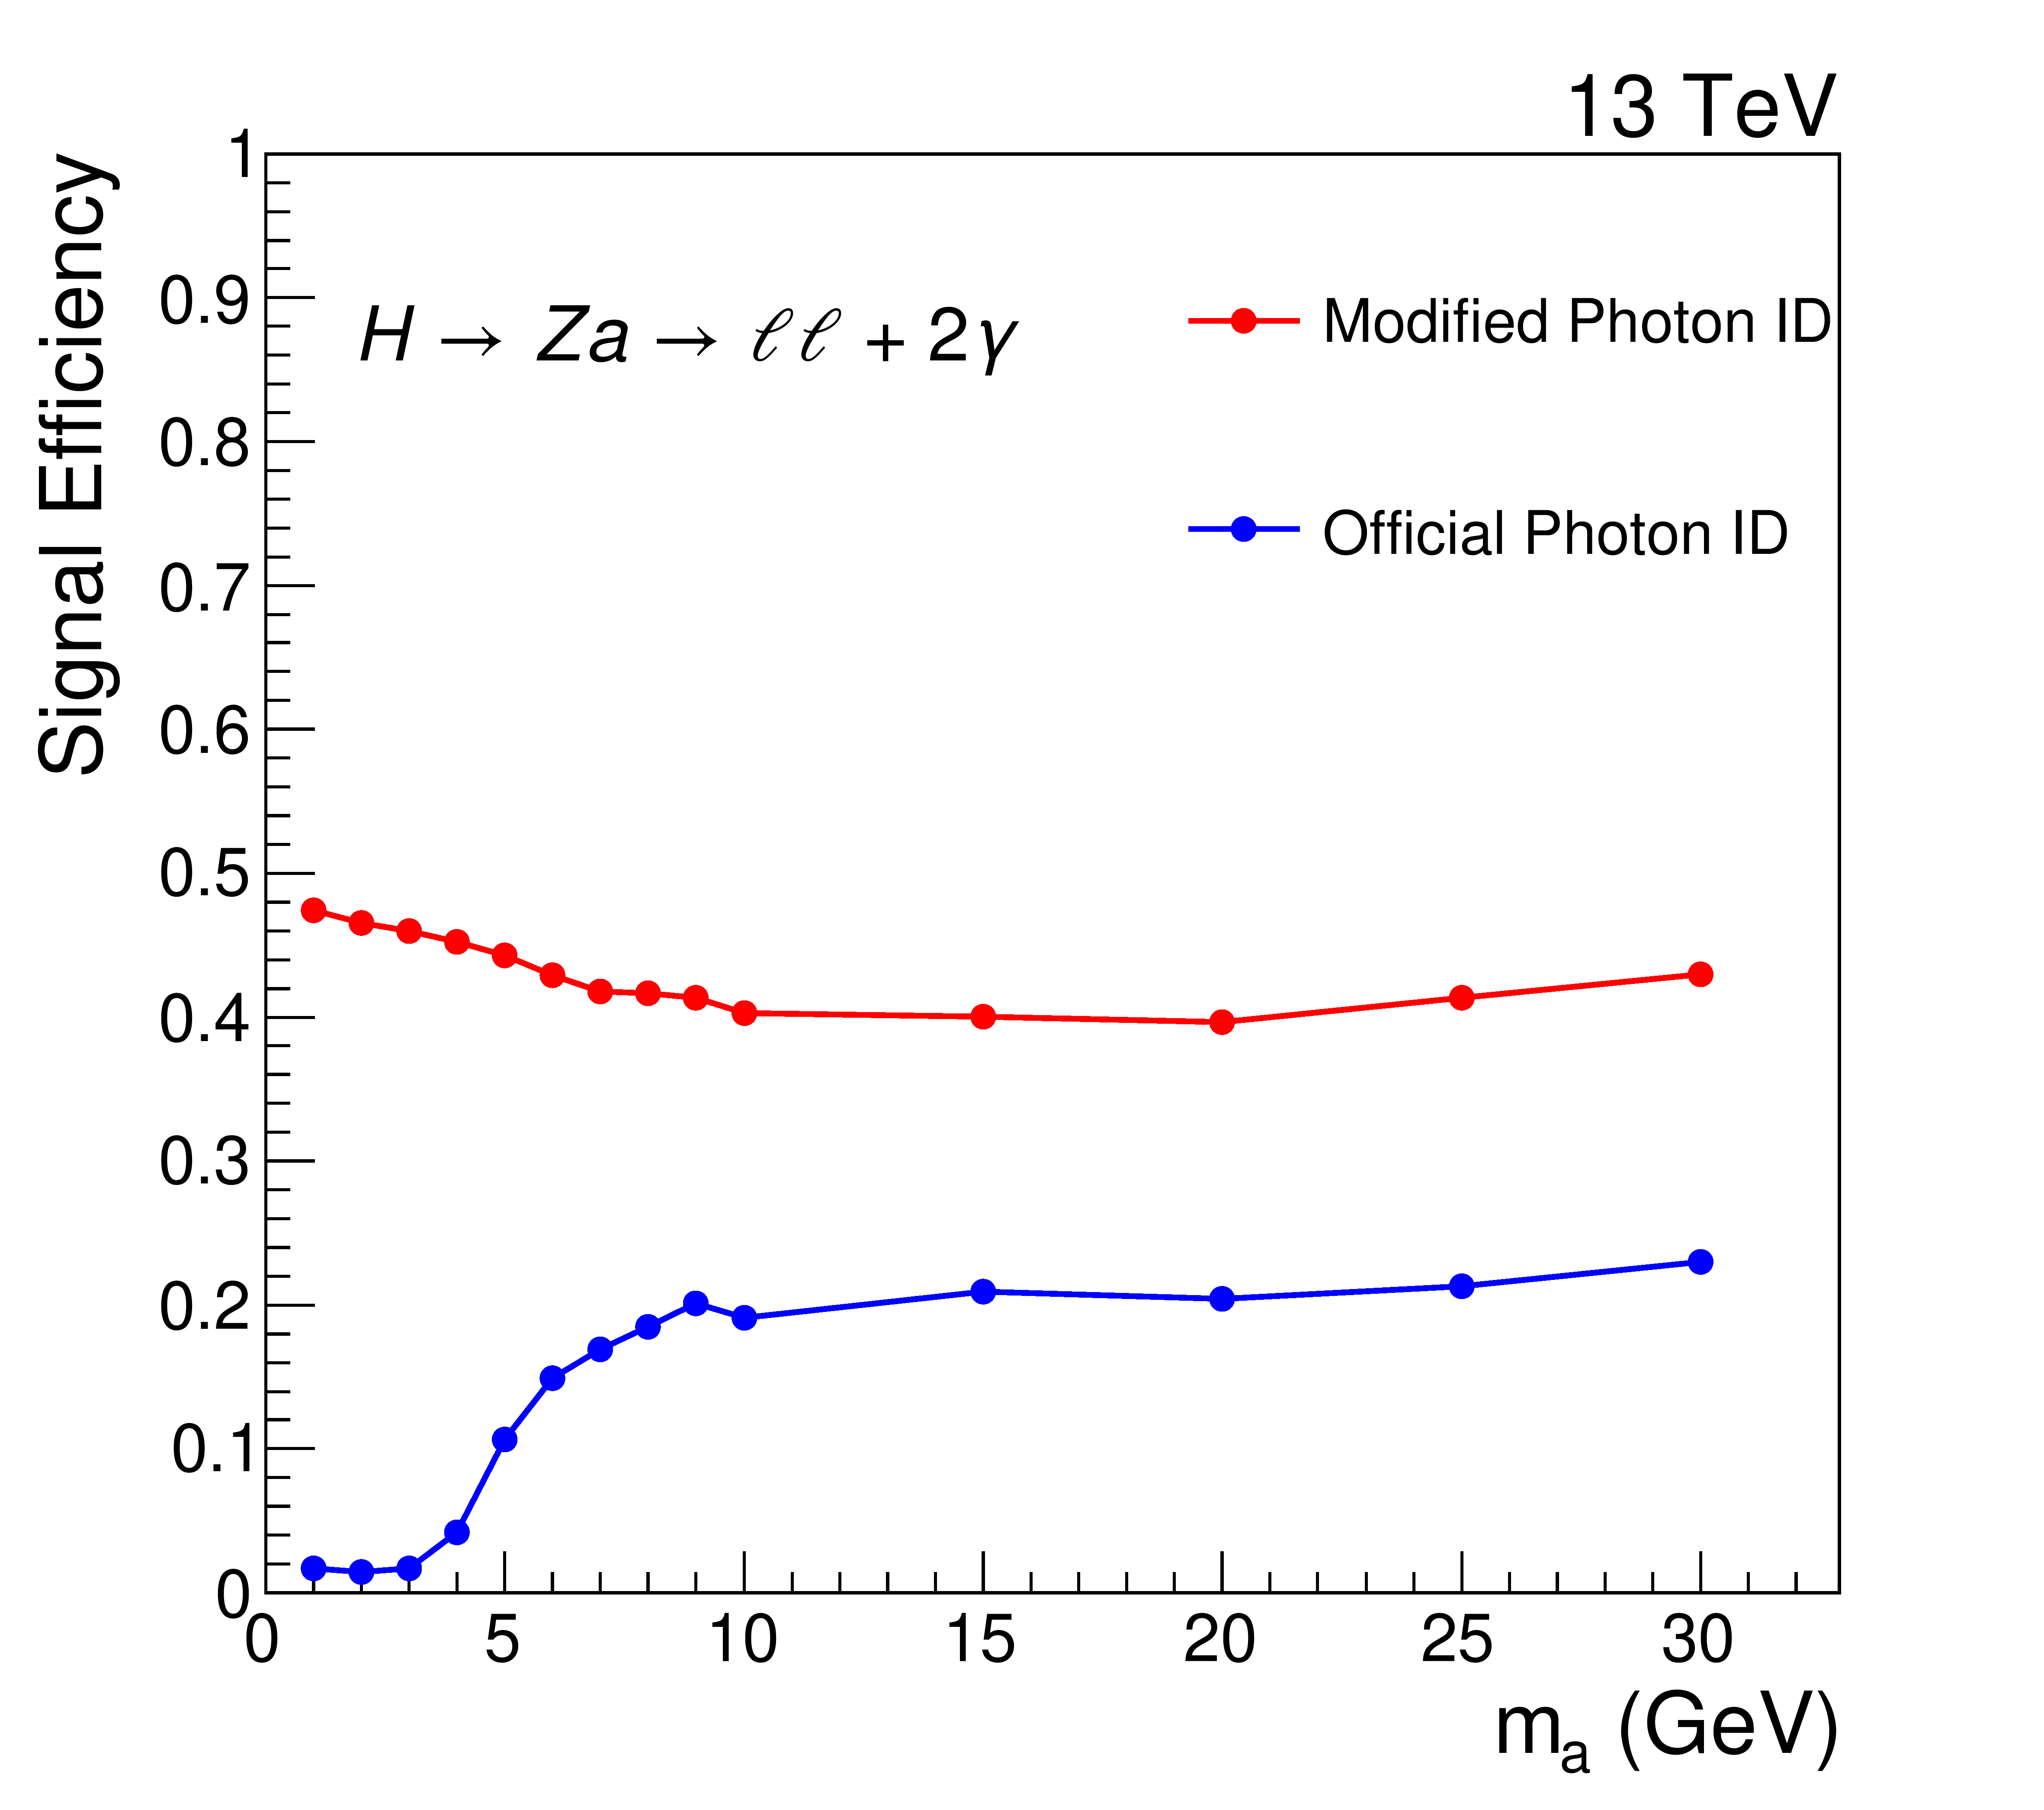
\includegraphics[width=0.45\textwidth]{figures/chapter04/ID_eff.png} \\
    \bicaption{\quad \centering 官方cut-based photon ID和新设计的ID之间信号效率的对比}{\quad \centering The comparison of signal efficiency between the official cut-based photon ID and the newly designed ID}
    \label{fig:IDCorr_eff}
\end{center}
\end{figure}


\subsection{筛选效率测量}\label{subsec:PhoTagProbe}

以上对电子、缪子和光子物理对象的筛选所造成的数据和蒙卡之间的差异可以通过利用tag-and-probe(T\&P)的方法计算出对应的比例因子(Scale Factors,SFs)来对蒙卡进行修正。T\&P方法是一种基于数据驱动(Data-driven)的技术,可以用于测量对应的探测效率。这种方法主要基于对已知的几种共振态衰变到我们所研究的特定粒子对的理解,比如$\mathrm{J/\psi}$、$\Upsilon$和Z衰变到电子对或者缪子对。

在任何物理分析中,确定探测器的效率具有至关重要的作用,它表明了对撞中产生的粒子有多少没有被探测器所接收,原因可能是来自于产生的粒子没有到达探测器探测单元或者没有被重建算法所识别等等。通常情况下,探测效率可以利用蒙卡模拟进行估算,但是由于蒙卡模拟并不完美,模拟和数据之间总是会存在微小的差异,这时就需要利用数据对蒙卡模拟进行刻度修正,T\&P方法正是一种可以直接从数据中提取效率的方法。

在这个方法中,可以利用已知的共振态衰变到特定粒子对来对探测效率进行测量。比如说可以利用$Z\rightarrow ee$的样本来对电子的选择效率进行测量,我们将衰变产生的两个电子一个定义为tag电子,另一个定义为probe电子,对它们定义的评判标准如下:

\begin{itemize}
    \item Tag电子:具有良好识别性的真电子,往往要求这个电子通过严格的筛选条件。
    \item Probe电子:没有偏差的电子候选体,往往要求这个电子通过非常宽松的筛选条件,它可以是通过或者没有通过我们将要测量的筛选条件的任何电子。
\end{itemize}
由于我们利用了特定的$Z\rightarrow ee$样本,样本中的所有事例绝大部分都是由Z衰变所产生的两个电子,tag电子的选择可以反向作为$Z\rightarrow ee$事例的触发,可以确保筛选出来的$Z\rightarrow ee$事例的纯度。而另一个probe电子的筛选是为了尽可能的保留的$Z\rightarrow ee$事例,并且可以用这个电子作为测量效率的工具。

探测效率的定义如下:
\begin{equation}
    \varepsilon = \frac{N_{pass}}{N_{total}}
\end{equation}
其中,$N_{pass}$表示通过筛选条件的probe电子的事例数,$N_{total}$指的是所有probe电子的事例数,是所有通过和未通过筛选条件的probe电子数总和。由于数据中没有办法完全排除本底,直接使用事例数所得到的探测效率往往会有较大的误差。但是由于tag-probe电子对的不变质量谱可以在Z玻色子的质量点处构成一个共振态,因此可以利用拟合数据的方法扣除本底的贡献,进而得到更为准确的探测效率。在分别得到对应数据和蒙卡之间的探测效率之后,由筛选条件所造成的数据和蒙卡之间的差异可以使用比例因子来对蒙卡样本进行修正,比例因子的定义如下:
\begin{equation}
    SFs = \frac{\varepsilon_{Data}}{\varepsilon_{MC}}
\end{equation}
其中,$\varepsilon_{Data}$指的是数据的测量效率,$\varepsilon_{MC}$指的是蒙卡的测量效率。SFs的计算往往可以分为不同的$\pt-\eta$区间,在不同的$\pt-\eta$区间内分别计算探测效率和对应的SFs可以得到更为准确的结果。

由电子的loose筛选和tight筛选所造成的数据和蒙卡样本之间的差异可以利用上述方法计算对应的SFs并将其应用到蒙卡样本的修正中解决。本分析所使用的电子loose cut比例因子由CMS实验官方提供,而电子的tight cut所对应的比例因子由CMS实验$H\rightarrow ZZ\rightarrow 4\ell$物理分析组~\cite{cmsHZZ}提供,图~\ref{fig:EleIDEff}展示了整个Run2三年的电子SFs测量结果以及对应的不确定性。

\begin{figure}[htbp]
  \begin{center}
		\includegraphics[width=0.7\textwidth,page=3]{figures/chapter04/2016_egammaEffitxt_egammaPlots.pdf}
    \includegraphics[width=0.75\textwidth,page=3]{figures/chapter04/2017_egammaEffitxt_egammaPlots.pdf} \\
		\includegraphics[width=0.7\textwidth,page=3]{figures/chapter04/2018_egammaEffitxt_egammaPlots.pdf}
    \bicaption{\quad \centering 左边:所有数据相对于模拟的电子SFs作为$\pt$和$\eta$的函数。右边:数据相对于模拟的电子SFs的不确定性作为$\pt$和$\eta$的函数。顶部显示了2016年的结果,中间显示了2017年的结果,底部显示了2018年的结果}{\quad \centering Left: Overall data to simulation scale factors for electrons, as function of $\pt$ and $\eta$. Right: Uncertainties on  data to simulation scale factors for electrons, as a function of $\pt$ and $\eta$. Results are shown for 2016 (top), 2017 (middle), and 2018 (bottom)}
    \label{fig:EleIDEff}
\end{center}
\end{figure}

利用以上方法,我们也可以对缪子的探测效率进行测量,唯一的不同就是所使用的样本是$Z\rightarrow \mu\mu$过程。而对于低$\pt$的缪子效率测量,由于$\mathrm{J/\psi}$的质量相比于Z玻色子小很多,衰变产生的两个缪子的$\pt$会比较小,因此可以利用$\mathrm{J/\psi}\rightarrow\mu\mu$的样本来对低动量区域的缪子进行效率测量。图~\ref{fig:MuonIDEff}展示了整个Run2三年的缪子SFs测量结果以及对应的不确定性。

\begin{figure}[htbp]
  \begin{center}
		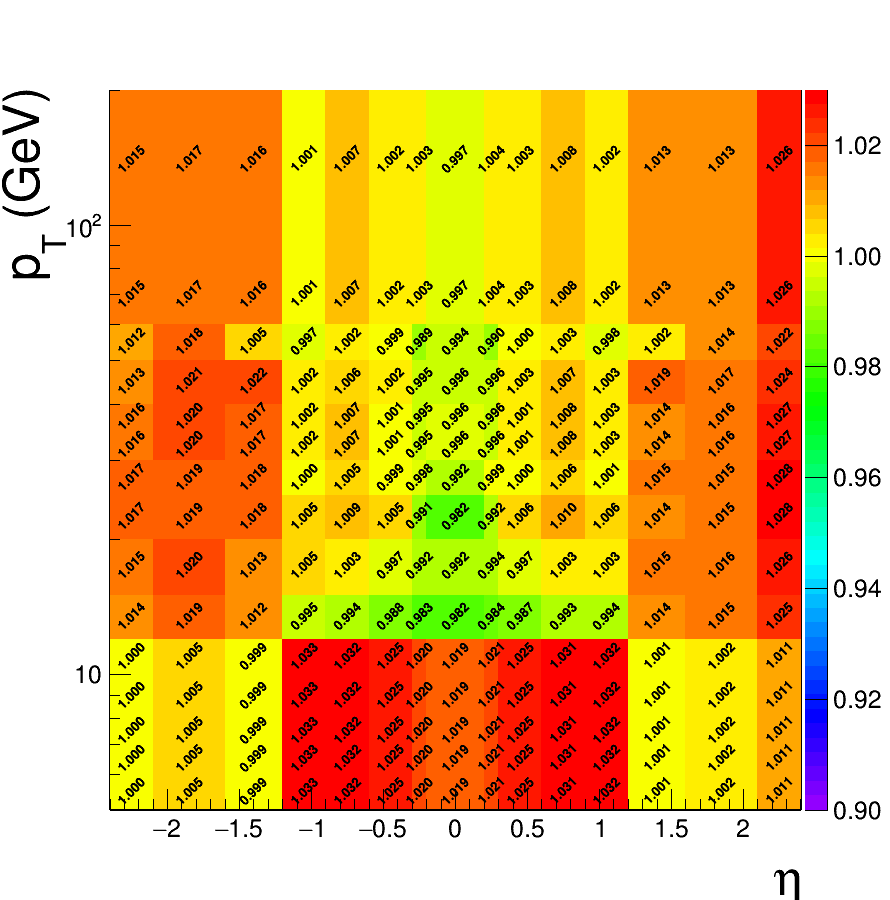
\includegraphics[width=0.45\textwidth]{figures/chapter04/2016_SF_legacy_newLoose.png}
    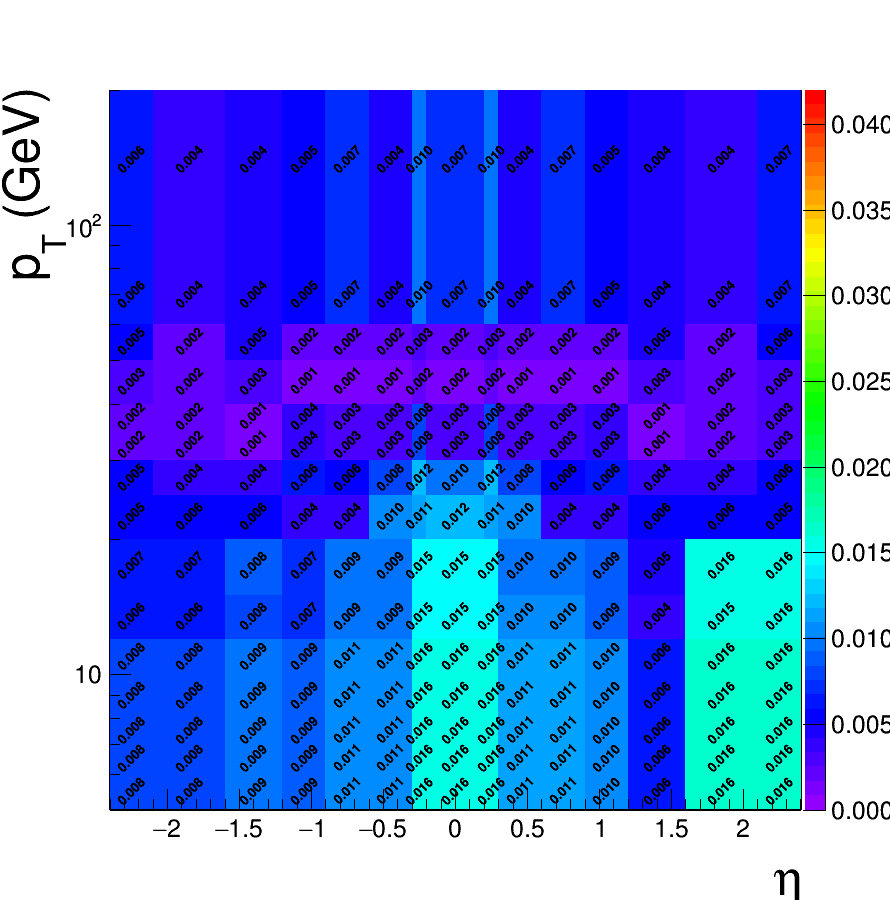
\includegraphics[width=0.45\textwidth]{figures/chapter04/2016_SF_errors_legacy_newLoose.png} \\
		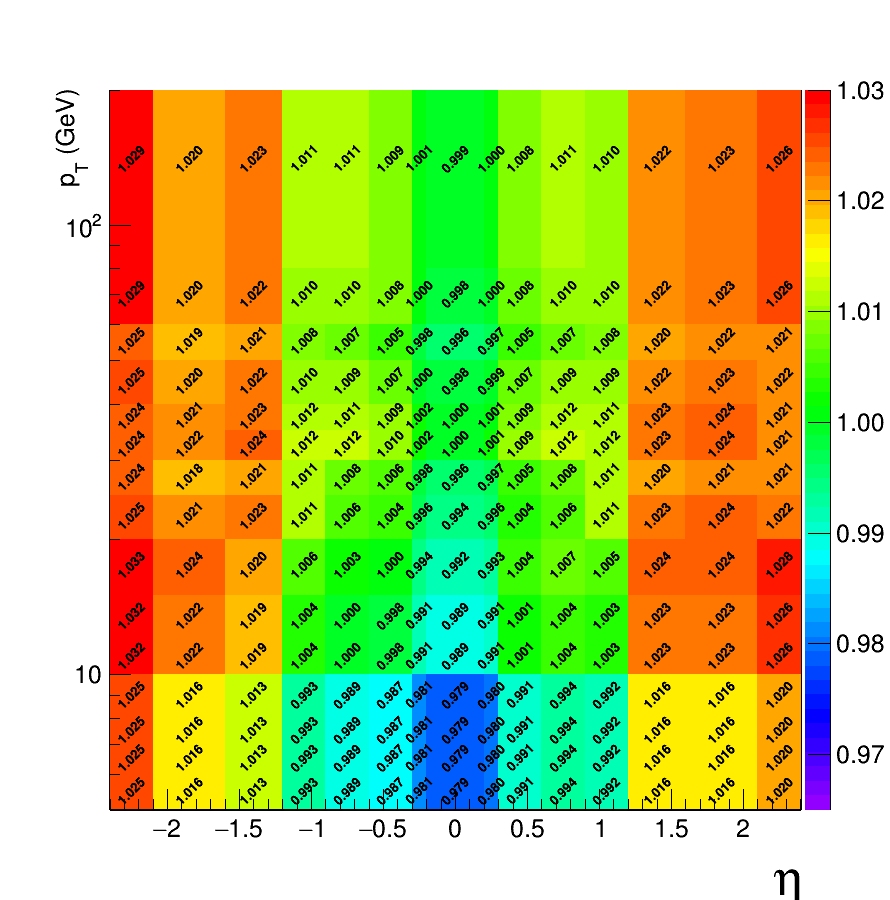
\includegraphics[width=0.45\textwidth]{figures/chapter04/2017_SF_rereco_LooseGT20syst.png}
    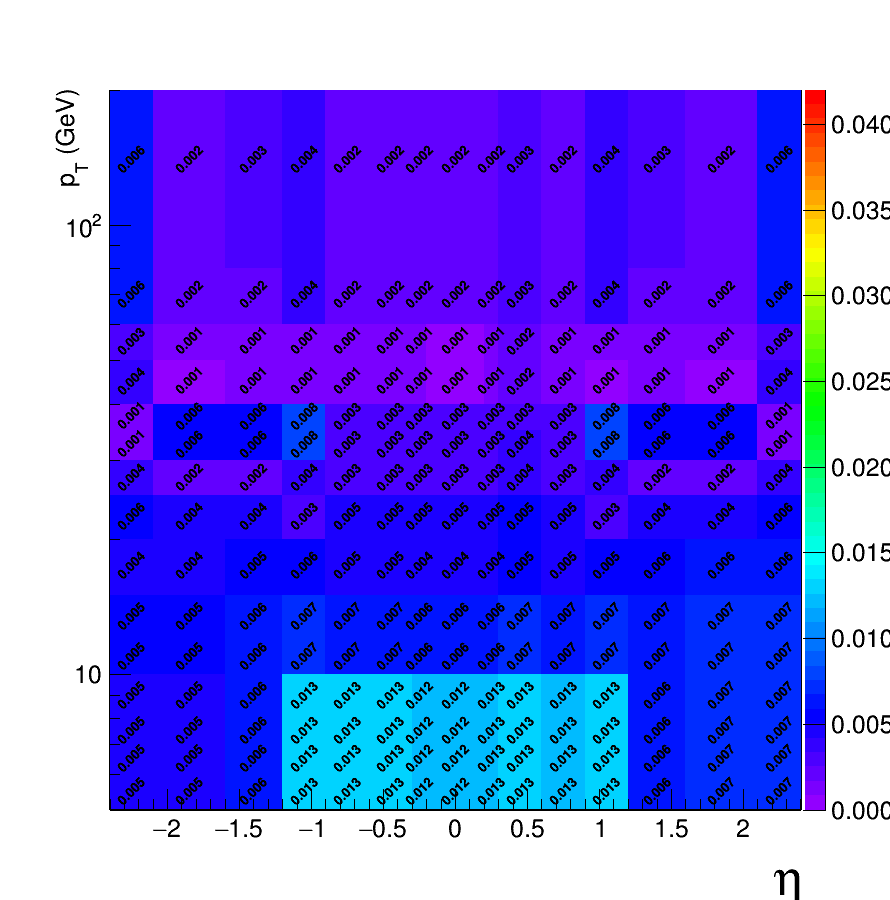
\includegraphics[width=0.45\textwidth]{figures/chapter04/2017_SF_errors_rereco_LooseGT20syst.png} \\
		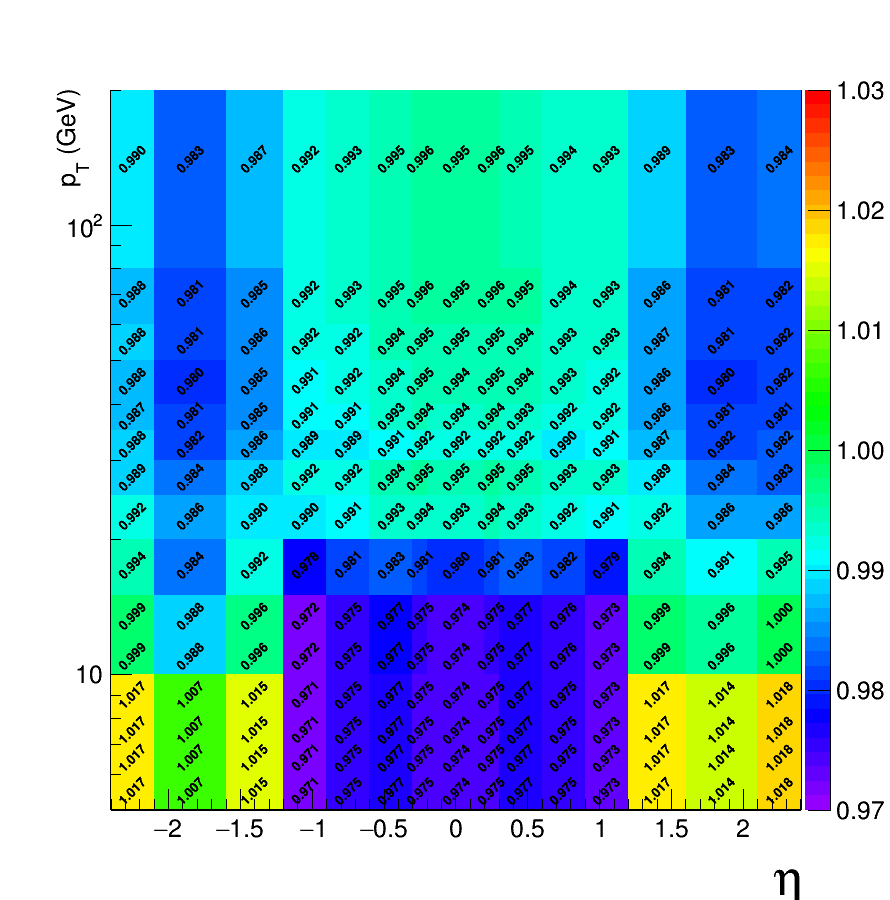
\includegraphics[width=0.45\textwidth]{figures/chapter04/2018_SF_rereco_LooseGT20syst.png} 
		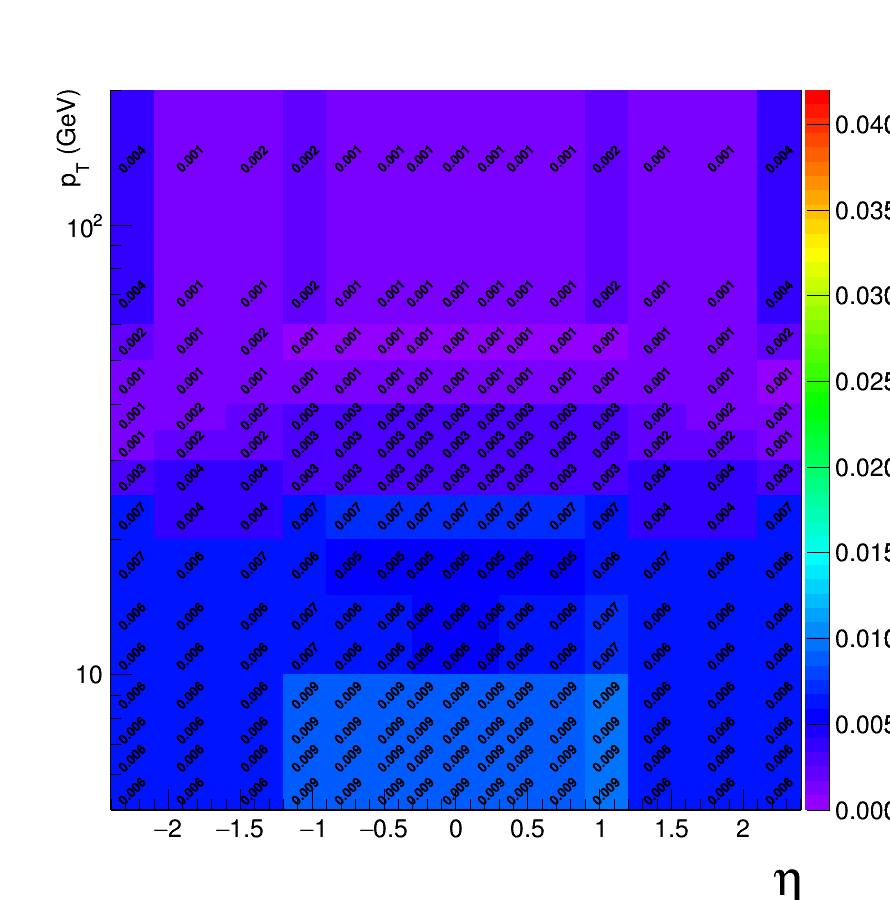
\includegraphics[width=0.45\textwidth]{figures/chapter04/2018_SF_errors_rereco_LooseGT20syst.png}
    \bicaption{\quad \centering 左边:所有数据相对于模拟的缪子SFs作为$\pt$和$\eta$的函数。右边:数据相对于模拟的缪子SFs的不确定性作为$\pt$和$\eta$的函数。顶部显示了2016年的结果,中间显示了2017年的结果,底部显示了2018年的结果}{\quad \centering Left: Overall data to simulation scale factors for muons, as function of $\pt$ and $\eta$. Right: Uncertainties on  data to simulation scale factors for muons, as a function of $\pt$ and $\eta$. Results are shown for 2016 (top), 2017 (middle), and 2018 (bottom)}
    \label{fig:MuonIDEff}
\end{center}
\end{figure}

而对于光子效率的测量,由于在CMS探测器中电子和光子的重建过程几乎完全相同,唯一的区别就是电子会在中心径迹室留下轨迹。因此,我们仍然可以利用$Z\rightarrow ee$的事例来对光子进行效率测量,唯一的区别就是我们使用的是由电子所假扮的假光子。为了满足这一要求,我们只需将由中心径迹室所决定的conversion-safe electron veto这一要求应用到电子上,就可以得到用于光子测量的假光子。

\begin{table}[h]
    \centering
    \bicaption{\quad \centering 用于测量光子效率所使用的样本}{\quad \centering Samples used for photon efficiencies measurement}
    \resizebox{\textwidth}{!}{
    \begin{tabular}{ll} \hline
        Datasets & File name \\ \hline
       2016 pre-VFP & [1]UL2016\_SingleEle\_Run2016[B,C,D,E,F].root \\ 
        & [1]DYJetsToLL\_M-50\_TuneCP5\_13TeV-madgraphMLM-pythia8\_preVFP\_UL2016.root \\ 
        & [1]DYJetsToLL\_M-50\_TuneCP5\_13TeV-amcatnloFXFX-pythia8\_preVFP\_UL2016.root \\ \hline
       2016 post-VFP & [2]UL2016\_SingleEle\_Run2016[F\_postVFP, G, H] \\ 
      & [2]DYJetsToLL\_M-50\_TuneCP5\_13TeV-madgraphMLM-pythia8\_postVFP\_UL2016.root \\ 
      & [2]DYJetsToLL\_M-50\_TuneCP5\_13TeV-amcatnloFXFX-pythia8\_postVFP\_UL2016.root \\ \hline
      2017 & [3]SingleEle\_Run[B,C,D,E,F].root \\
        & [3]DYJetsToEE.root \\ 
        & [3]DYJetsToLL\_amcatnloFXFX.root\\ \hline
        2018 & [4]EGamma\_Run[A,B,C,D].root \\ 
        & [4]DYJetsToLL\_madgraphMLM.root \\ 
        & [4]DYJetsToLL\_amcatnloFXFX.root \\ \hline
       \multicolumn{2}{l}{[1] = /eos/cms/store/group/phys\_egamma/akapoor/Tag-and-Probe\_Tree/UL2016\_ntuples/}\\
       \multicolumn{2}{l}{[2] = /eos/cms/store/group/phys\_egamma/akapoor/Tag-and-Probe\_Tree/UL2016\_ntuples/}\\
       \multicolumn{2}{l}{[3] = /eos/cms/store/group/phys\_egamma/asroy/Tag-and-Probe\_Tree/UL2017\_MINIAOD\_Nm1/}\\
       \multicolumn{2}{l}{[4] = /eos/cms/store/group/phys\_egamma/asroy/Tag-and-Probe\_Tree/UL2018\_MINIAOD\_Nm1/}
    \end{tabular}}
    \label{tab:TnP_datasets}
\end{table}

列表~\ref{tab:TnP_datasets}展示了本分析中光子效率测量所使用的样本,事例中的所有电子都通过conversion-safe electron veto这一要求。本分析中对新设计的光子ID效率的测量所使用的tag和probe电子的选择如下:
\begin{itemize}
    \item Tag电子:通过tight工作点,$\pt>35\GeV$并且$|\eta|<2.17$;
    \item Probe电子:$\pt>10\GeV$;
    \item 两个电子的不变质量位于60$\GeV$和120$\GeV$之间;
\end{itemize}
通过利用信号加本底的模型对双轻子的不变质量谱进行拟合可以得到对应的筛选效率。其中,拟合中的信号模型使用的是蒙卡样本中的信号模型和一个高斯函数的卷积,高斯函数主要是为了考虑探测器分辨率的影响;本底信号模型使用的是误差函数和指数函数的卷积。通过对拟合中的信号部分进行积分求和可以得到通过和未通过新设计的光子ID的事例数,从而可以得到数据和蒙卡的效率,它们之间的比值就作为蒙卡修正所使用的SFs。在本分析中,效率和SFs的测量是在以下$\pt$和$\eta$的范围中计算的:
\begin{itemize}
    \item $\pt$:10$\GeV$,15$\GeV$,20$\GeV$,35$\GeV$,50$\GeV$;
    \item $|\eta|$:0.0,0.8,1.4442,1.566,2.0,2.5;
\end{itemize}

图~\ref{fig:IDCorr_eff_fit}展示了2018年数据中效率测量的一个拟合结果,这个结果是在$-2.5<\eta<2.0$ 和 $10<\pt<15$~\si{GeV}的范围内进行测量的。其中,passing probe表示的是通过新设计的光子ID的tag-probe电子对不变质量分布图,failing probe表示没有通过的tag-probe电子对不变质量分布图。黑色的点表示数据,蓝色和红色的曲线分别表示拟合得到的本底模型和信号模型。通过对红色曲线下的面积求和就可以得到对应的通过和未通过的probe电子事例数,进而可以得到对应的效率值。然后再利用数据和蒙卡之间的效率值之比就可以得到对应区间的SFs。

\begin{figure}[htbp]
  \begin{center}
    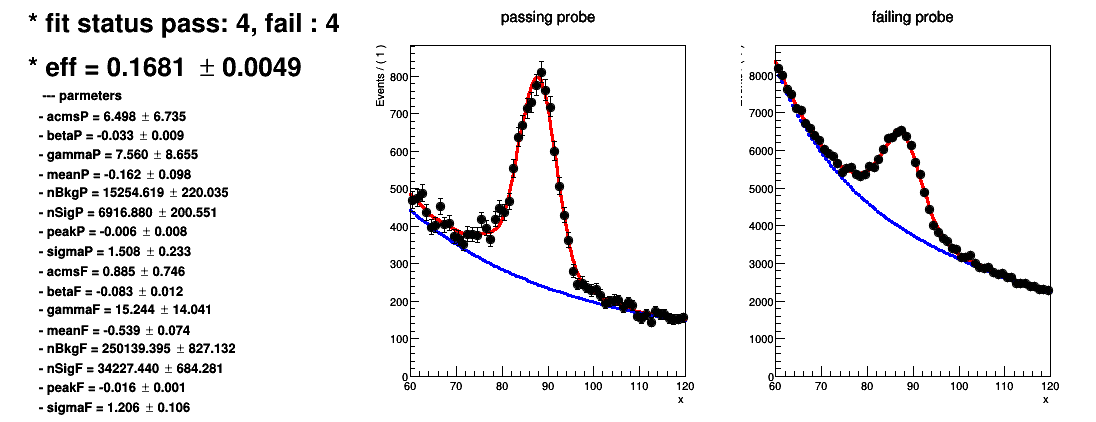
\includegraphics[width=1.0\textwidth]{figures/chapter04/bin00_ph_sc_eta_m2p50Tom2p00_ph_et_10p00To15p00.png}
    \bicaption{\quad \centering 2018年数据中效率测量在$-2.5<\eta<2.0$ \&\& $10<\pt<15$~\si{GeV}范围内的拟合结果}{\quad \centering The fitting results of the efficiency measurement in 2018 data within the bins of $-2.5<\eta<2.0$ \&\& $10<\pt<15$~\si{GeV}}
    \label{fig:IDCorr_eff_fit}
\end{center}
\end{figure}

\begin{figure}[htbp]
  \begin{center}
		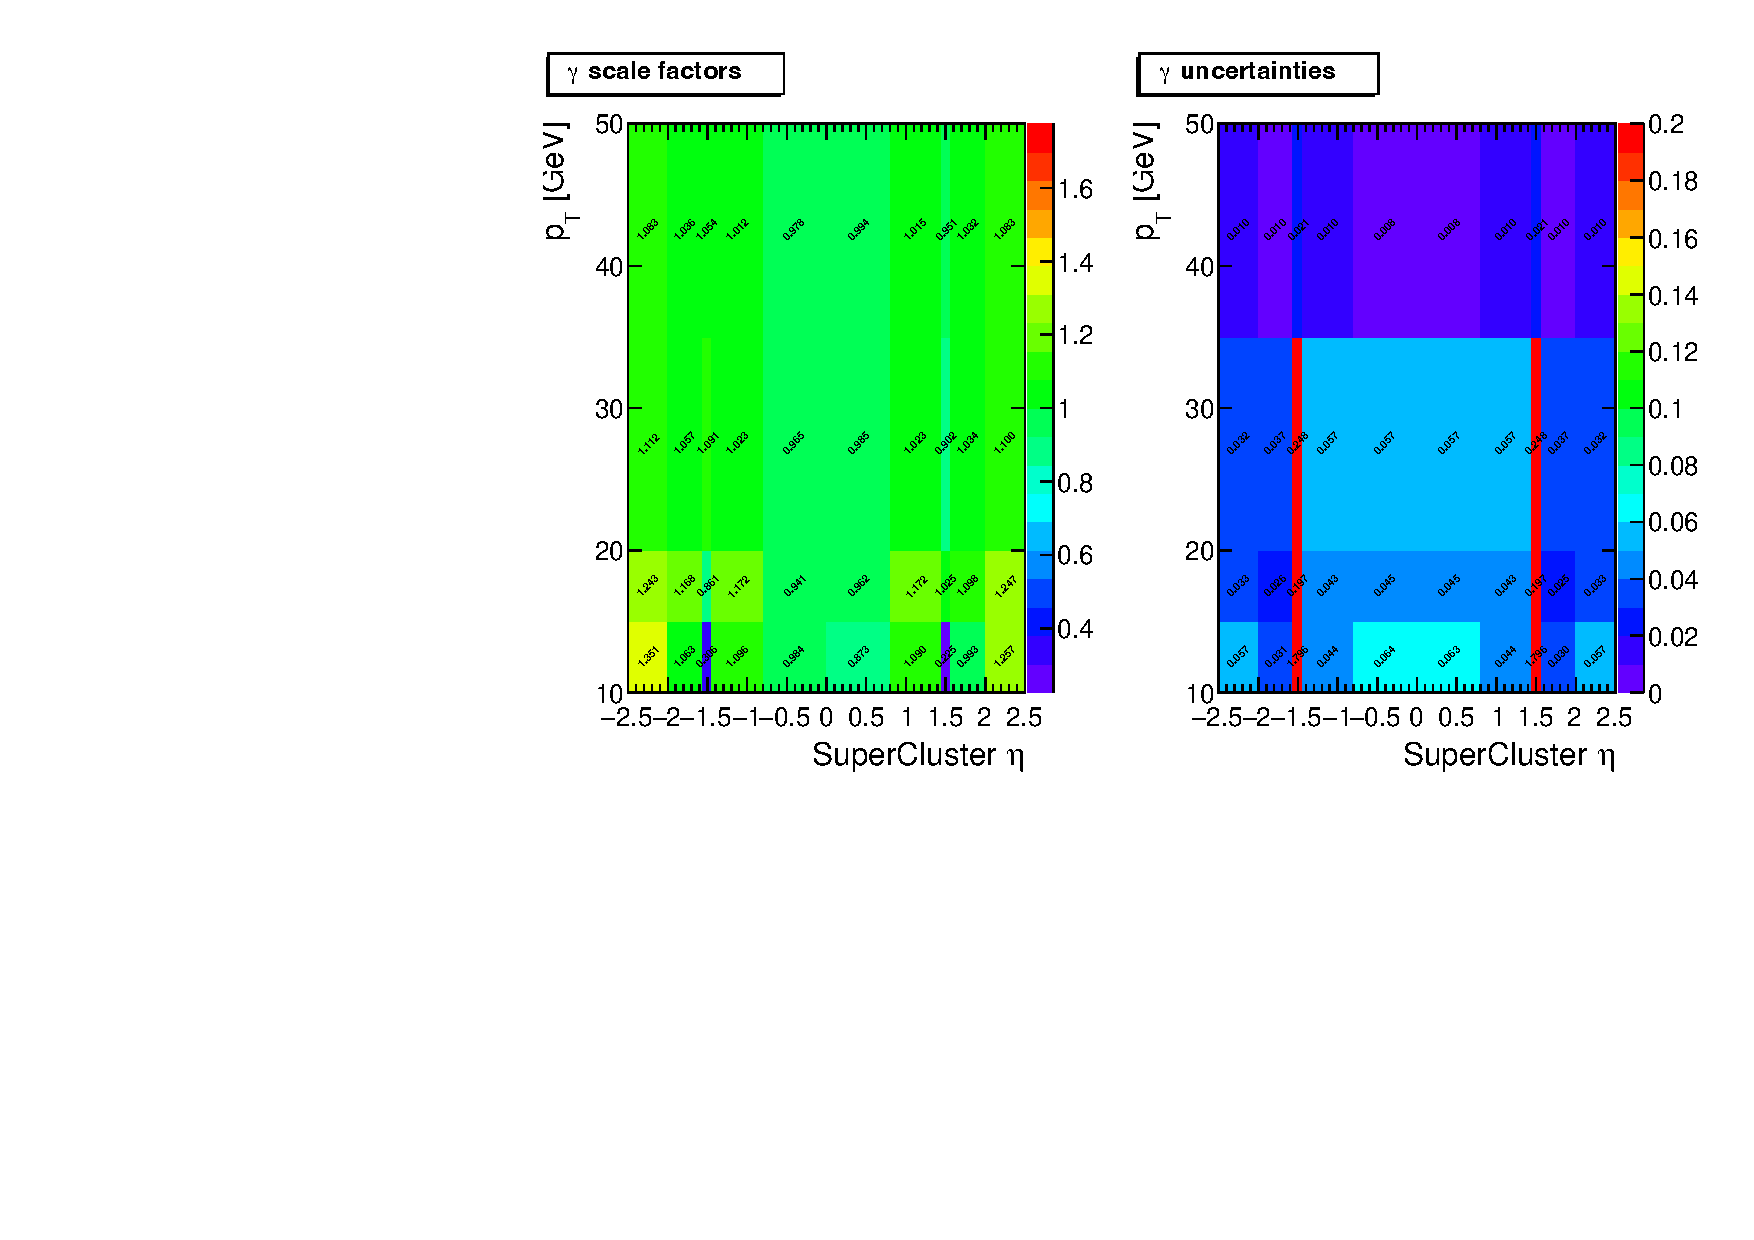
\includegraphics[width=0.8\textwidth]{figures/chapter04/phoID_eff_2016preVFP.pdf}\\
    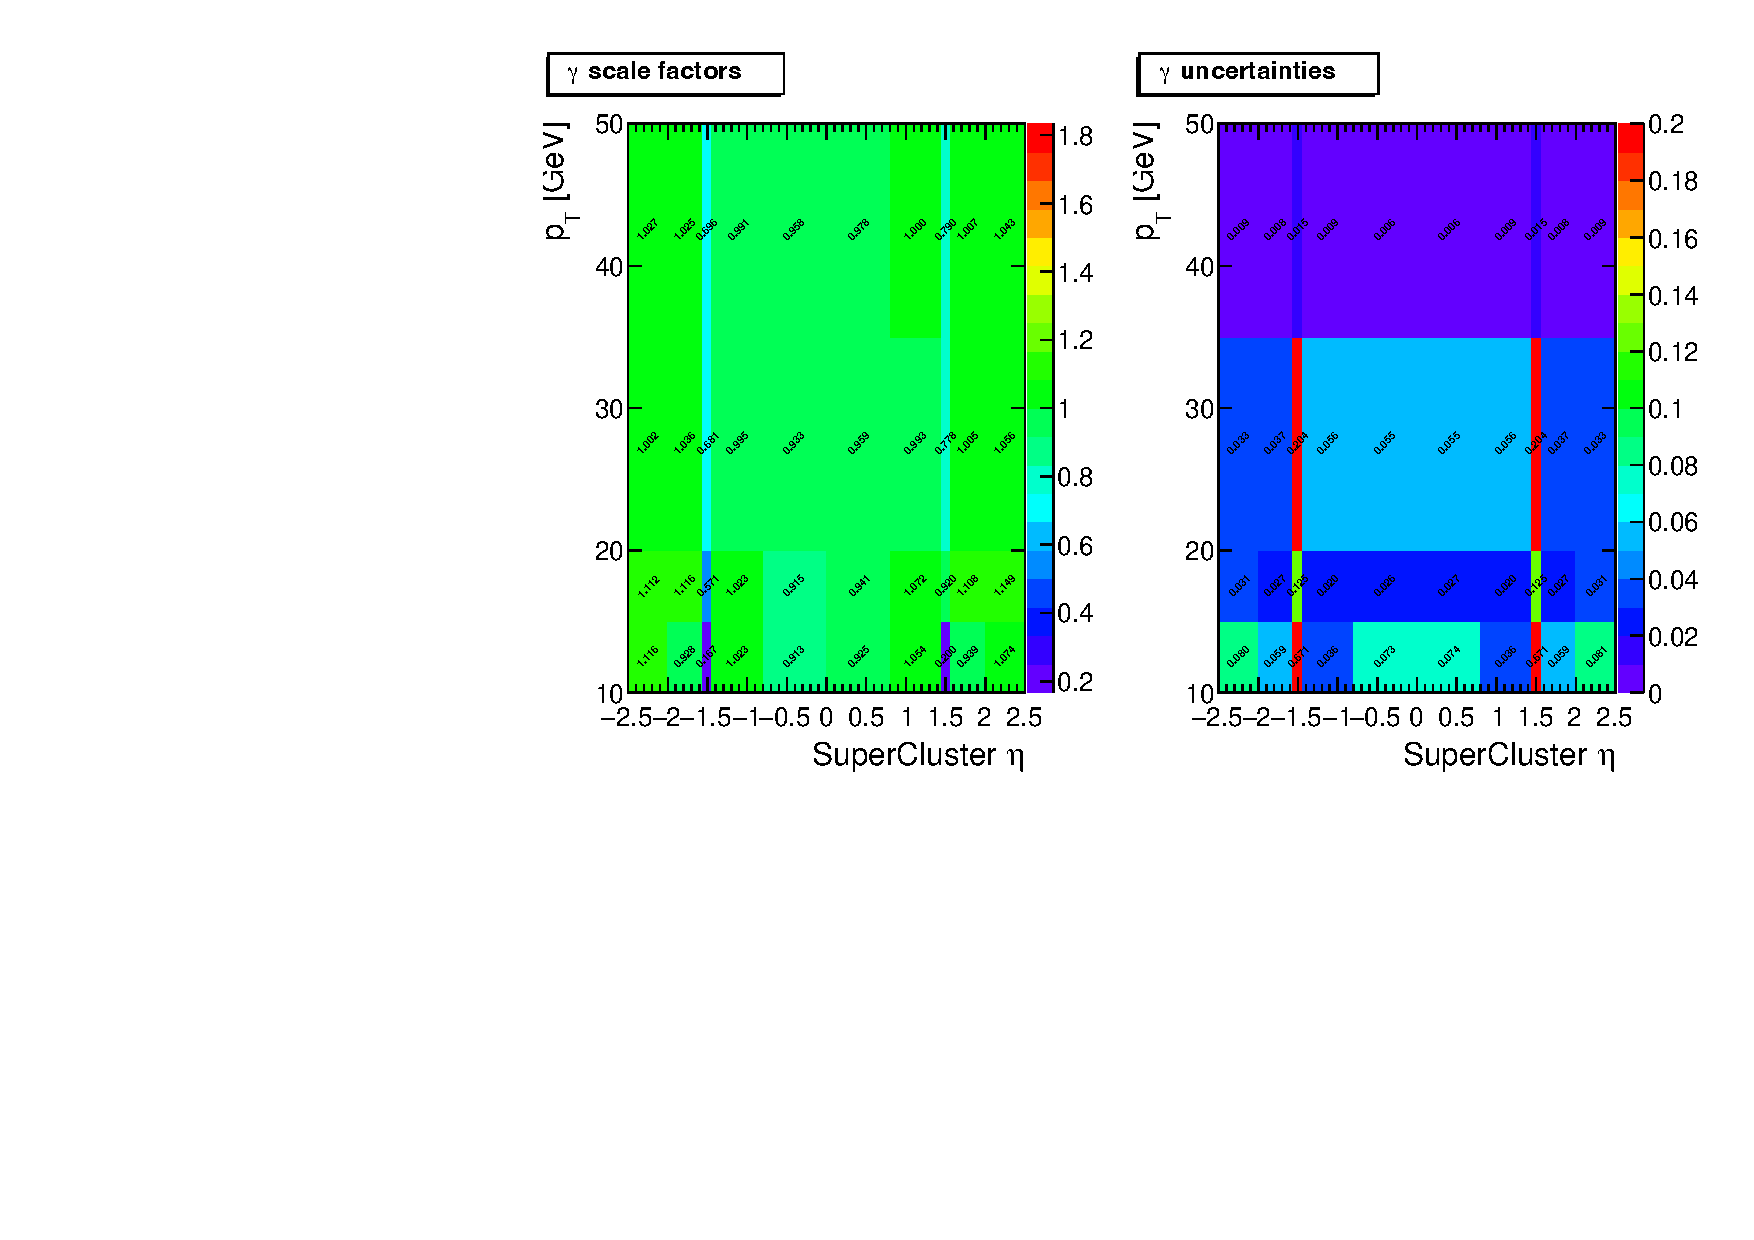
\includegraphics[width=0.8\textwidth]{figures/chapter04/phoID_eff_2016postVFP.pdf} \\
    \bicaption{\quad \centering 左边:所有数据相对于模拟的光子SFs作为$\pt$和$\eta$的函数。右边:数据相对于模拟的光子SFs的不确定性作为$\pt$和$\eta$的函数。顶部显示了2016年pre-VFP的结果,底部显示了2016年post-VFP的结果}{\quad \centering Left: Overall data to simulation scale factors for photons, as function of $\pt$ and $\eta$. Right: Uncertainties on data to simulation scale factors for photons, as a function of $\pt$ and $\eta$. Results are shown for 2016 pre-VFP (top), 2016 post-VFP (bottom)}
    \label{fig:PhoIDEff_1}
\end{center}
\end{figure}

\begin{figure}[htbp]
  \begin{center}
		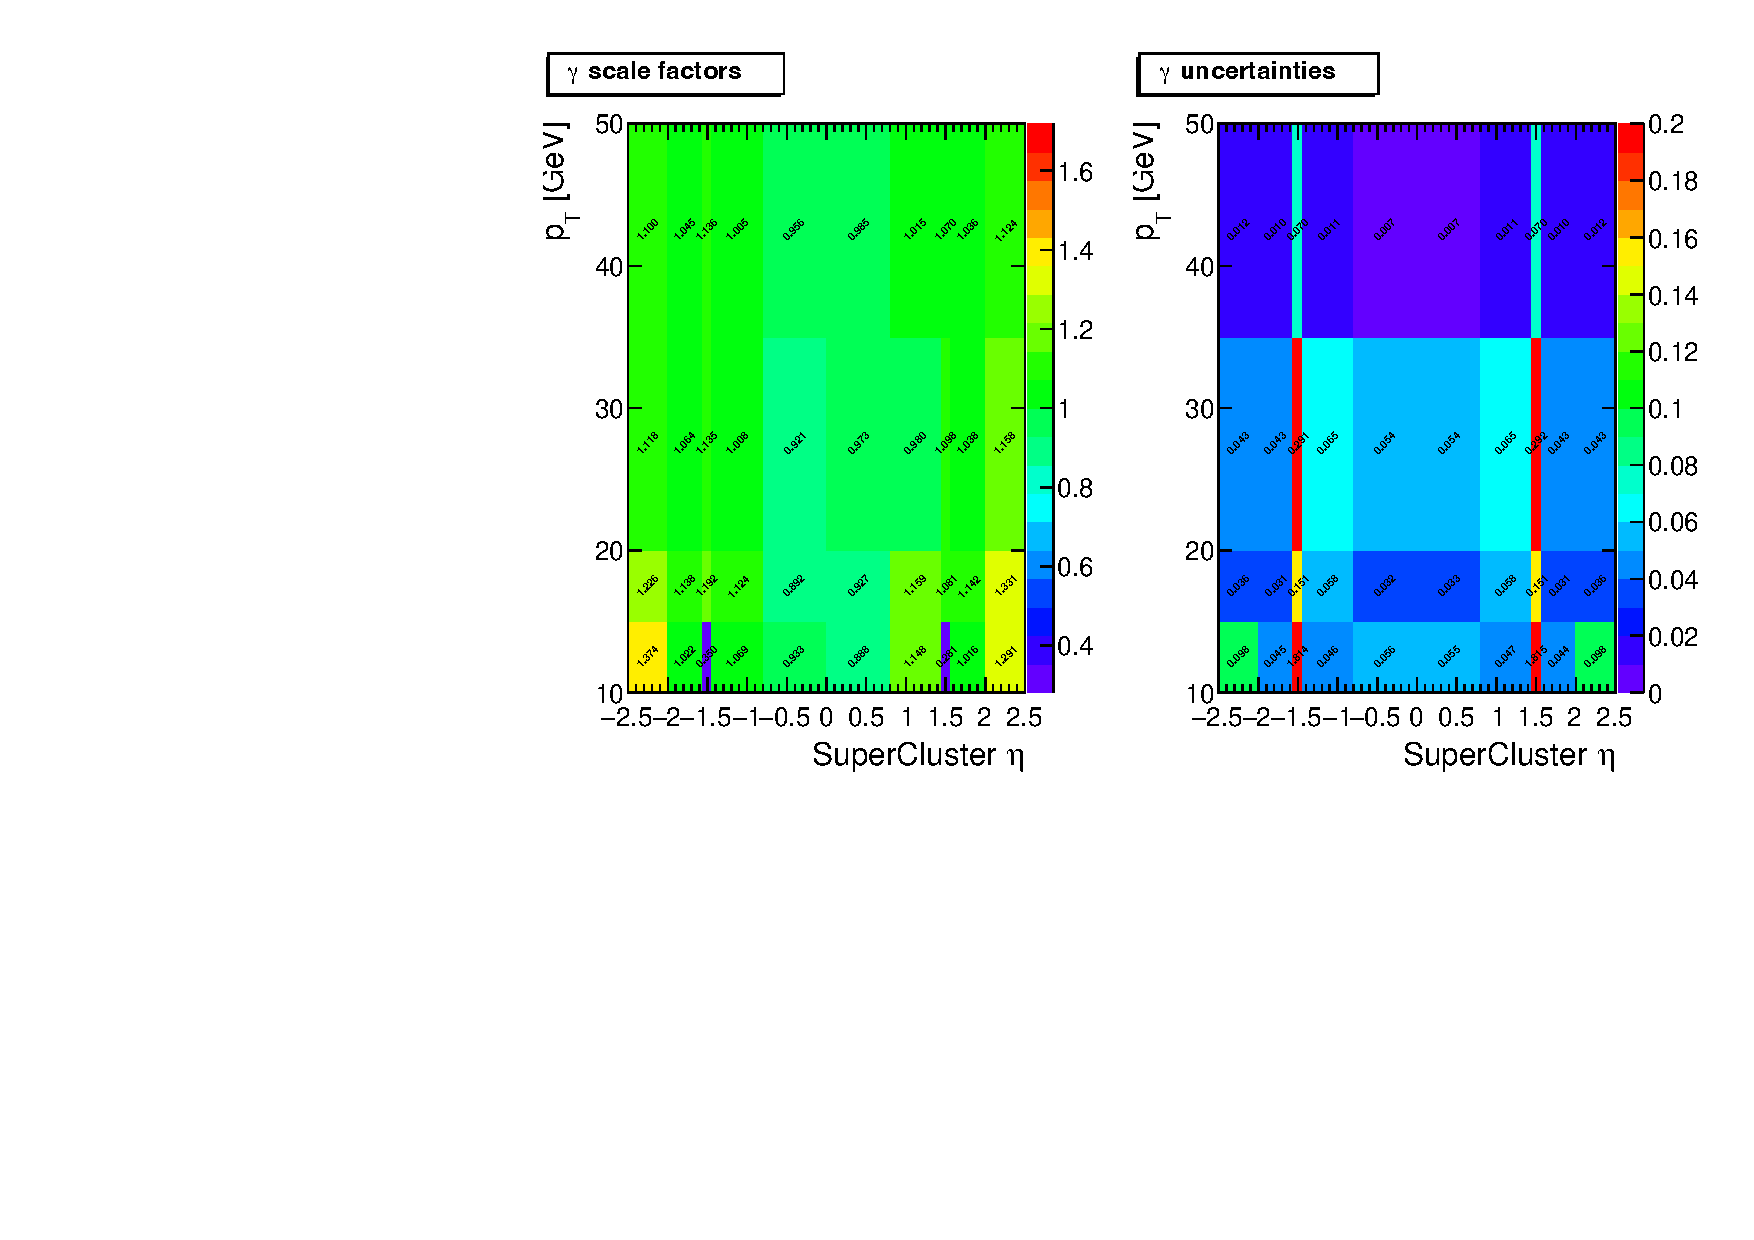
\includegraphics[width=0.8\textwidth]{figures/chapter04/phoID_eff_2017.pdf}\\
		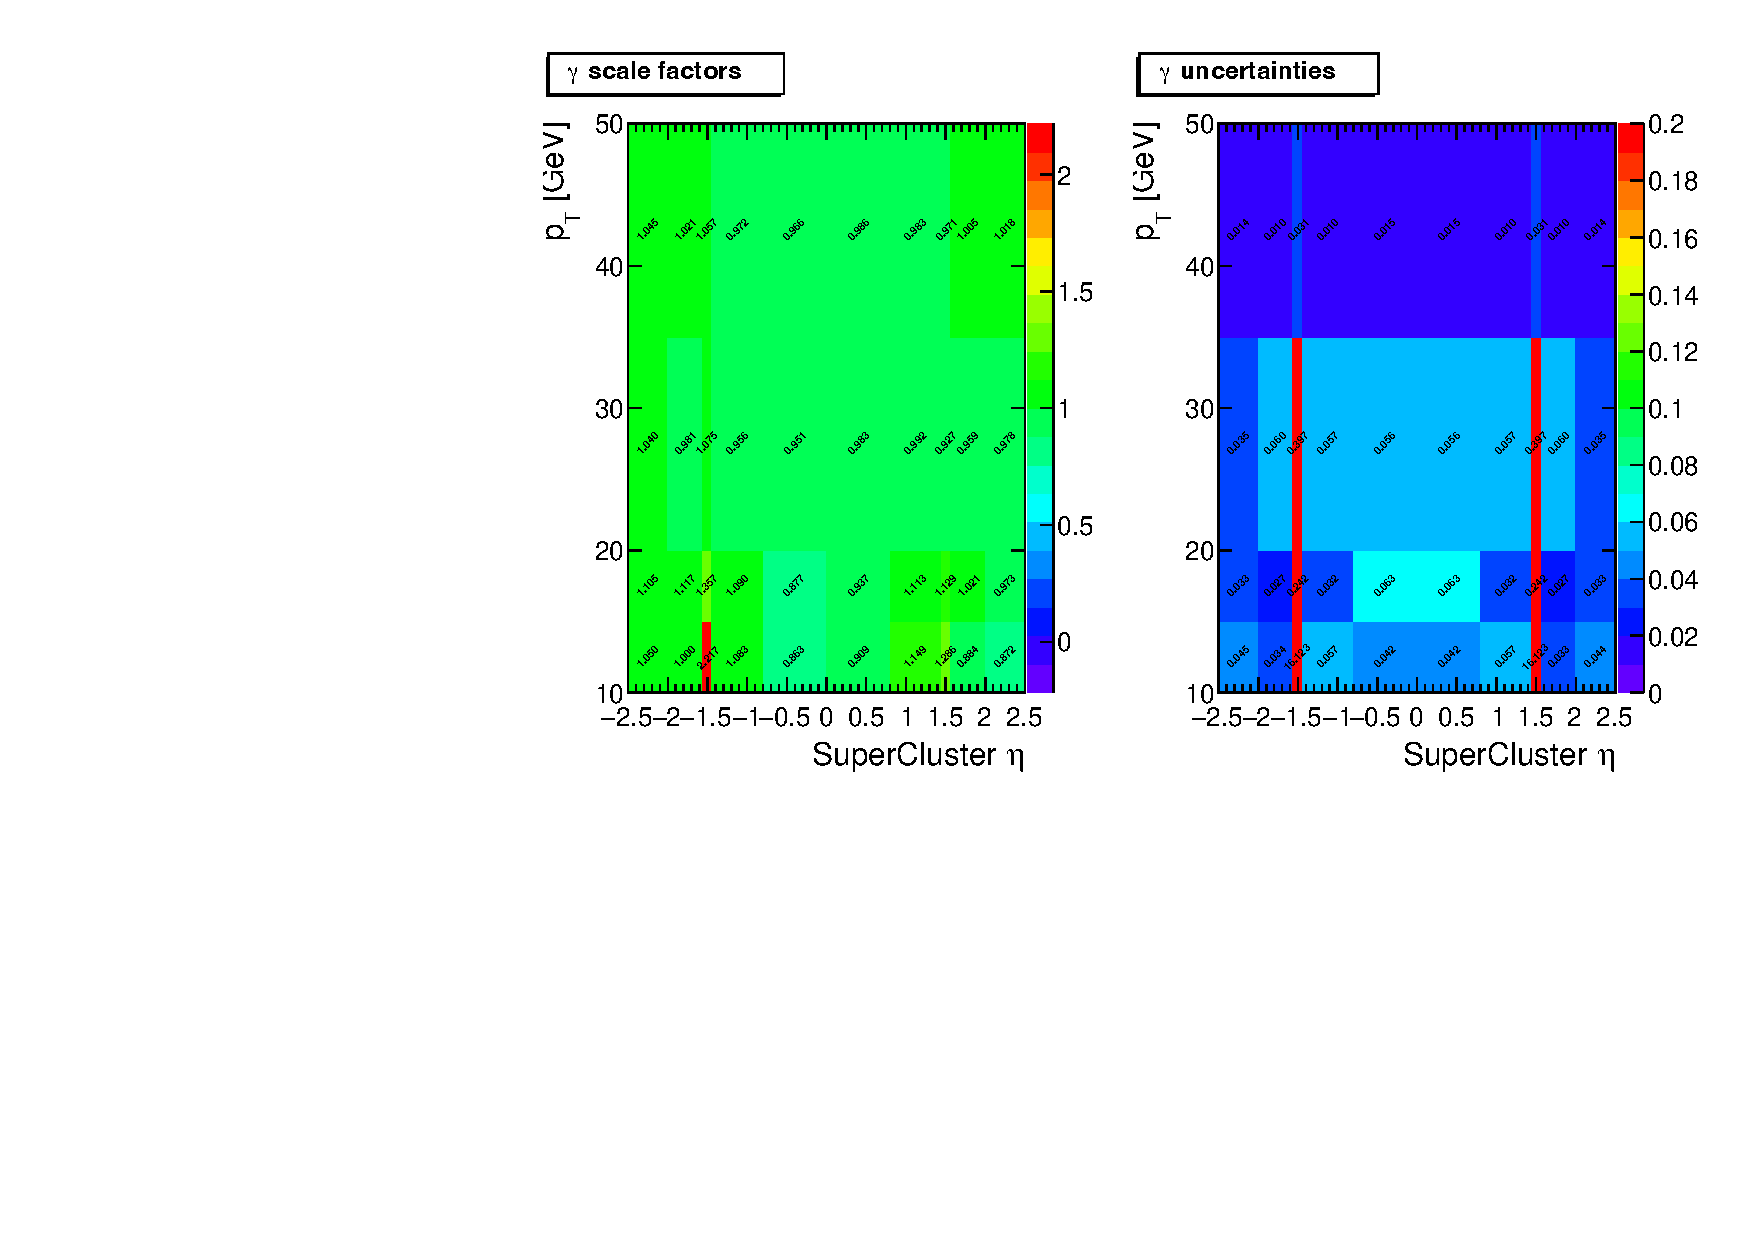
\includegraphics[width=0.8\textwidth]{figures/chapter04/phoID_eff_2018.pdf}\\
    \bicaption{\quad \centering 左边:所有数据相对于模拟的光子SFs作为$\pt$和$\eta$的函数。右边:数据相对于模拟的光子SFs的不确定性作为$\pt$和$\eta$的函数。顶部显示了2017年的结果,底部显示了2018年的结果}{\quad \centering Left: Overall data to simulation scale factors for photons, as a function of $\pt$ and $\eta$. Right: Uncertainties on data to simulation scale factors for photons, as a function of $\pt$ and $\eta$. Results are shown for 2017 (top) and 2018 (bottom)}
    \label{fig:PhoIDEff_2}
\end{center}
\end{figure}

图~\ref{fig:PhoIDEff_1}和图~\ref{fig:PhoIDEff_2}展示了整个Run2三年的SFs和对应的误差。其中,误差的计算考虑了以下来源:
\begin{itemize}
    \item 来自数据样本统计涨落的误差;
    \item 来自蒙卡样本统计涨落的误差;
    \item 来自本底模型的误差:拟合所使用的本底模型的形状会对最终的效率计算产生影响,进而影响最终的SFs。这部分误差可以通过使用不同形状的本底模型进行拟合来估算,在这个过程中信号模型保持不变,本底模型由原来的误差函数和指数函数的卷积改变为指数函数或者Power-Low函数。
    \item 来自信号模型的误差:拟合所使用的信号模型的形状同样也会对最终的SFs计算产生影响。与估计本底模型的误差相似,可以通过改变信号模型的形状来对这一部分误差进行估计。在这个过程中,本底模型的形状保持不变,信号模型由原来的蒙卡形状和高斯函数的卷积改变为Double Crystall Ball函数和高斯函数的卷积。
    \item 来自tag电子筛选引起的误差:这部分误差可以通过改变tag电子的筛选条件重新计算效率和SFs来进行估计。在估计的过程中,将tag电子的定义改变为通过medium工作点并且$\pt>25\GeV$。
    \item 来自蒙卡样本产生子引起的误差:使用不同的产生子产生出来的蒙卡样本会具有细微的差别。由于在拟合中信号模型利用了蒙卡样本的形状,因此使用不同产生子的蒙卡样本会影响最终的SFs的计算。这部分误差可以通过使用由不同产生子所产生的蒙卡样本来进行估算。
\end{itemize}

总的误差是以上所有误差来源项的平方和开根号。在本分析中,大部分光子的横动量都集中在30$\GeV$以下,对应的SFs的计算误差平均在5\%左右,其中占主导的误差来源是蒙卡样本产生子引起的误差。原因是由于Z玻色子衰变产生的电子横动量比较高,在低动量区域内的样本事例数比较少,统计涨落较大,因此更换不同产生子的蒙卡样本后会产生较大的影响。但是由于本分析是对Higgs稀有衰变过程的寻找,在最终的分析结果中数据的统计误差占主导,光子效率的误差仅产生次要的影响,详细分析结果见第~\ref{sec:Sys}节。

\section{事例筛选}\label{sec:EventSelect}

表格~\ref{tab:objsummary}总结了本分析中使用的所有物理对象的筛选条件,包括:电子、缪子、FSR光子以及光子。在对所有物理对象重建完成之后,可以利用这些物理对象重建出我们所感兴趣的事例。在本分析中,Higgs通过一个Z玻色子和一个类轴子作为中间态衰变到两个轻子加两个光子,因此可以通过两个轻子重建出Z玻色子、通过两个光子重建出类轴子,进而再利用Z玻色子和类轴子重建出Higgs粒子。具体重建步骤如下:
\begin{enumerate}
    \item Trigger 筛选:首先要求事例通过第~\ref{sec:Trigger}节描述的触发条件,要求筛选的事例含有至少一个轻子或者两个轻子。
    \item Z玻色子候选体筛选:要求事例含有至少一对味道相同带电相反的轻子($e^{+}e^{-}, \mu^{+}\mu^{-}$),这些轻子包含了相应的FSR光子并且通过了所有轻子的筛选条件。然后利用这些轻子对重建出Z玻色子候选体。其中,要求两个筛选出来的电子(缪子)满足$\mathrm{p_{T, Leading}>25 (20)\GeV}$,$\mathrm{p_{T, Sub-leading}>15 (10)\GeV}$,这些阈值的选择主要由触发决定。
    \item ALPs候选体筛选:要求事例中含有两个通过光子ID的光子,利用这两个光子重建出类轴子候选体。其中,要求这两个光子的横动量$\pt>10\GeV$,这主要是由CMS探测器中对光子重建所需的最低横动量所决定。
    \item Higgs候选体筛选:最后,利用Z玻色子候选体和类轴子候选体重建出Higgs候选体,选中的事例要求满足以下条件:
        \begin{itemize}
            \item Z玻色子的质量$m_{Z}>50\GeV$,用以排除$\gamma^{*}\rightarrow\ell\ell$这部分本底。
            \item 轻子和光子之间的距离$\dR(l,\gamma)>0.4$。
            \item 由于本分析要求一个在壳的Z玻色子和两个横动量大于10$\GeV$的光子,使得本底的$\mllgg$分布会在110$\GeV$附近出现了turn-on(不变质量谱的分布在110$\GeV$以下呈上升趋势,然后在110$\GeV$附近达到极大值,而后又呈下降趋势),为了使得本底建模的时候可以正确描述这部分turn-on并且拟合区间具有足够的边带区域,要求选出的Higgs候选体质量$95<\mllgg<180\GeV$。
        \end{itemize}
\end{enumerate}

\begin{table}[H]
	\centering
	\bicaption{\quad \centering 物理对象选择汇总}{\quad \centering Summary of physics object selection}
	\resizebox{\textwidth}{!}{
	\begin{tabular}{cc}
		\hline
		\multicolumn{2}{c}{\textbf{Electrons}} \\ \hline
		\multicolumn{2}{c}{$\mathrm{p_T^e} > 7 $~\si{\GeV} \hspace{0.5cm} $|\eta^e| < 2.5$}   \\
		\multicolumn{2}{c}{$\mathrm{d_{xy}} < 0.5 \, \mathrm{cm}$ \hspace{0.5cm} $\mathrm{d_{z}} < 1 \, \mathrm{cm}$}                  \\
		\multicolumn{2}{c}{$| {\rm SIP_{3D}} | < 4$ }  \\
        \multicolumn{2}{c}{BDTs ID with isolation with cuts }  \\ \hline \hline
		\multicolumn{2}{c}{\textbf{Muons}}  \\ \hline
        \multicolumn{2}{c}{Global or Tracker Muon} \\
		\multicolumn{2}{c}{$\mathrm{p_{T}^{\mu}} > 5$~\si{\GeV} \hspace{0.5cm} $|\eta^{\mu}| < 2.4$}   \\
		\multicolumn{2}{c}{$\mathrm{d_{xy}} < 0.5 \, \mathrm{cm}$ \hspace{0.5cm} $\mathrm{d_{z}} < 1 \, \mathrm{cm}$}           \\
		\multicolumn{2}{c}{$| {\rm SIP_{3D}} | < 4$  }  \\
		\multicolumn{2}{c}{PF muon ID if $\pt<200$~\si{\GeV}, PF muon ID or High-$\pt$ muon ID if $\pt>200$~\si{\GeV}}      \\
        \multicolumn{2}{c}{$\ensuremath{{\cal I}_{\mathrm{PF}}^{\mu}} < 0.35$}    \\ \hline \hline
		\multicolumn{2}{c}{\textbf{FSR photons}}    \\ \hline
		\multicolumn{2}{c}{$\mathrm{p_T^{\gamma}} > 2 \GeV$ \hspace{0.5cm} $|\eta^{\gamma}| < 2.4$}     \\
		\multicolumn{2}{c}{$\ensuremath{{\cal I}_{\mathrm{PF}}^{\gamma}} < 1.8$}        \\
		\multicolumn{2}{c}{$\Delta R(\ell,\gamma) < 0.5$ \hspace{0.5cm} $\frac{\Delta R(\ell,\gamma)}{(\pt^{\gamma})^2} < 0.012 \GeV^{-2}$}     \\ \hline \hline
		\multicolumn{2}{c}{\textbf{Photons}}    \\ \hline
		\multicolumn{2}{c}{$10 < \mathrm{p_T^{\gamma}} < 14 \GeV$ \hspace{0.2cm} $H/E < 0.15\ \&\&\ I_{ch} < 10\GeV$}     \\
		\multicolumn{2}{c}{or}     \\
		\multicolumn{2}{c}{$\mathrm{p_T^{\gamma}} > 14 \GeV$ \hspace{0.5cm} $H/E < 0.15$}     \\
		\multicolumn{2}{c}{Modified tight photon cut-based ID}     \\ \hline
	\end{tabular}}
	\label{tab:objsummary}
\end{table}

\begin{figure}[htbp]
  \begin{center}
		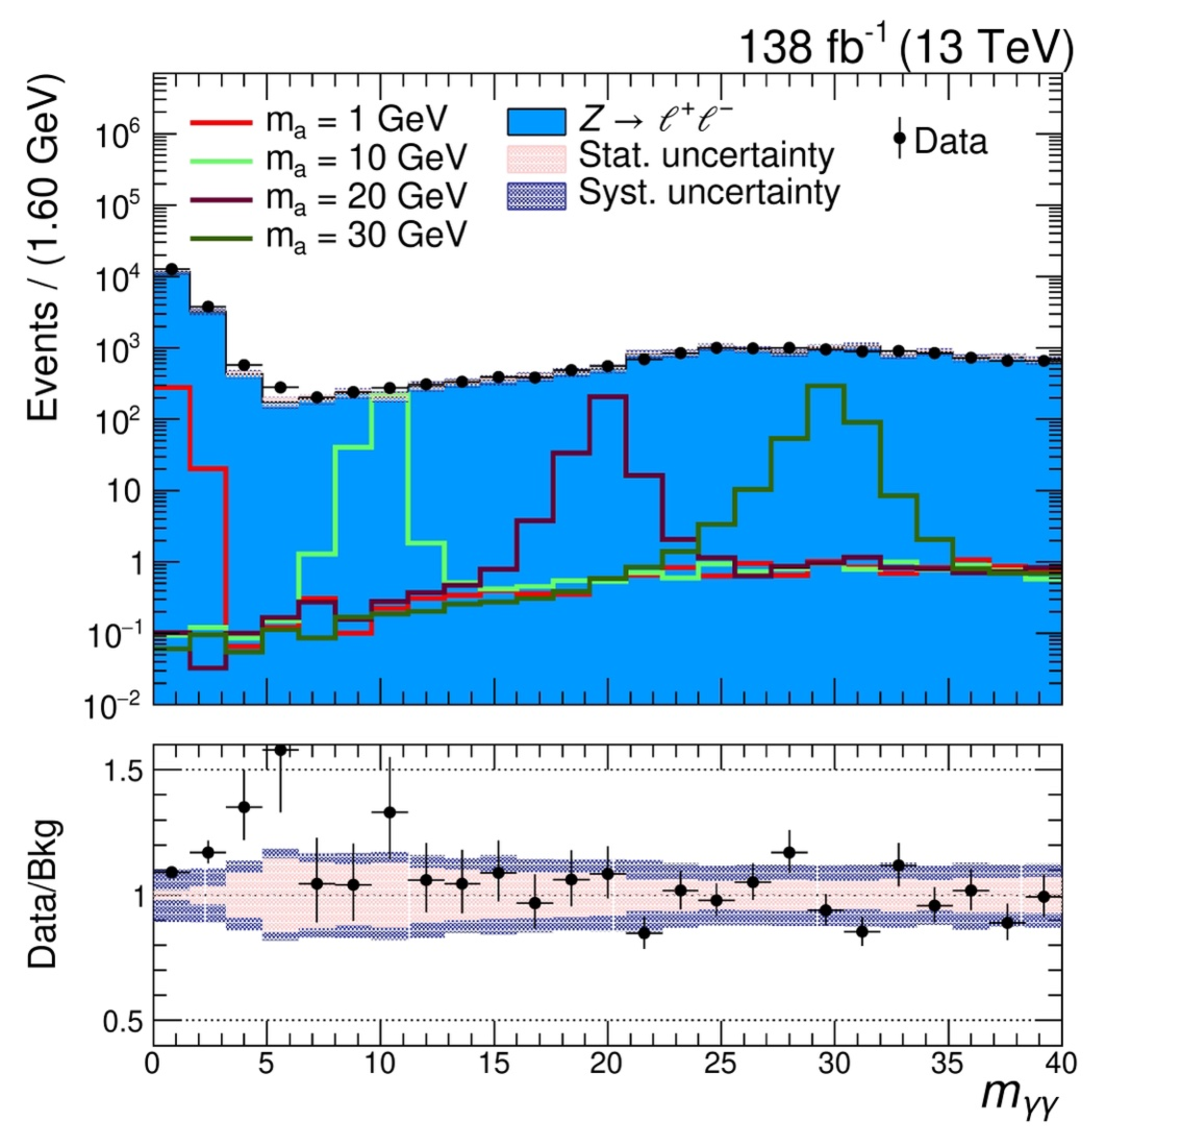
\includegraphics[width=0.5\textwidth]{figures/chapter04/BDT_input/ALP_m_log.pdf}
    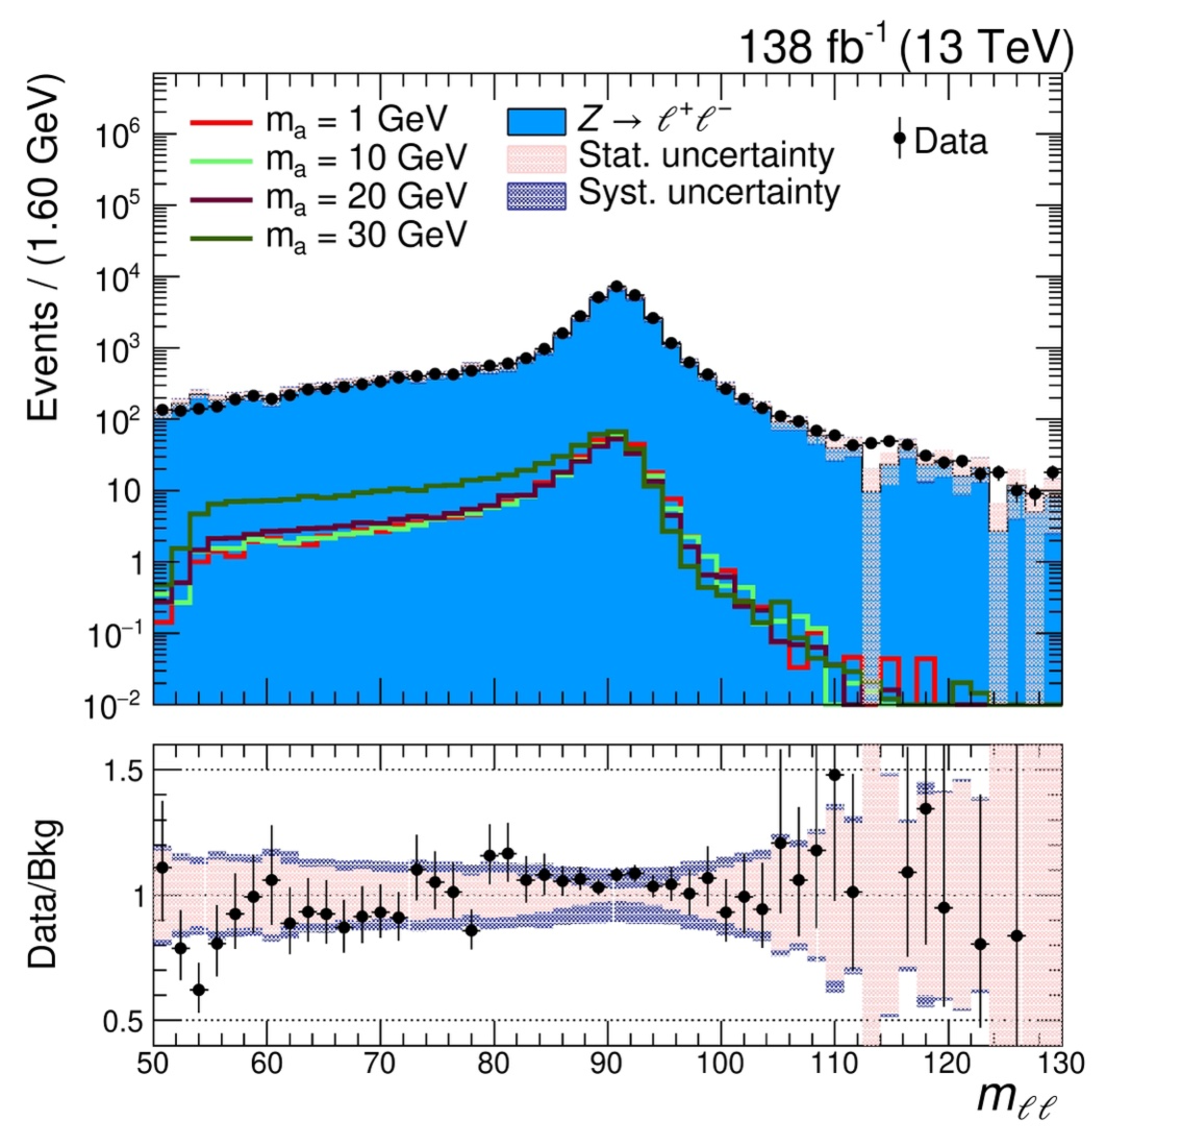
\includegraphics[width=0.5\textwidth]{figures/chapter04/BDT_input/Z_m_log.pdf} 
		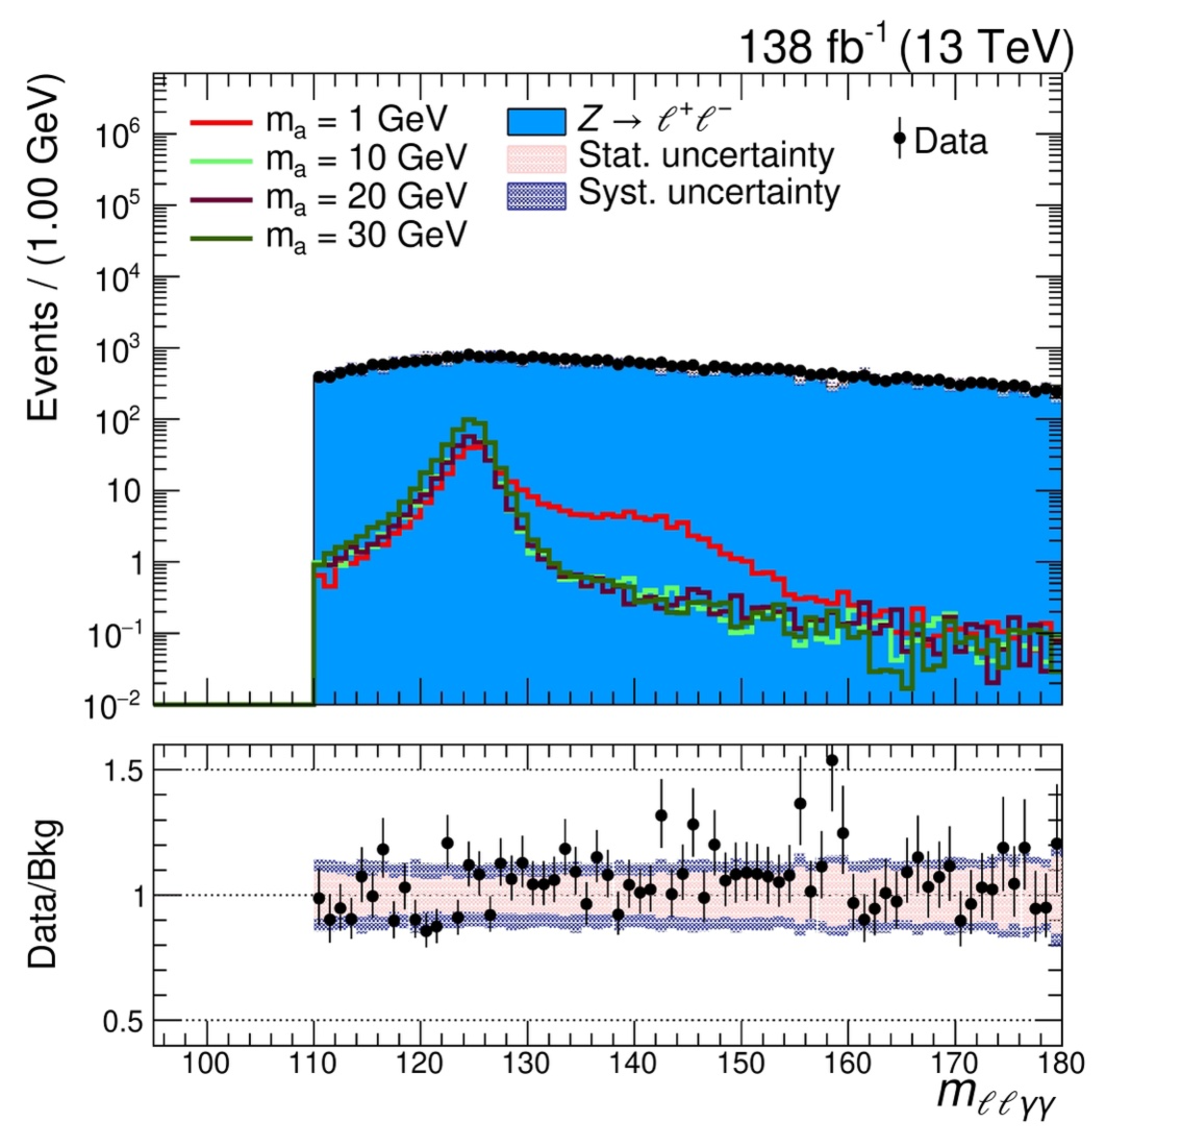
\includegraphics[width=0.5\textwidth]{figures/chapter04/BDT_input/H_m_log.pdf}
    \bicaption{\quad \centering 通过事例筛选后的ALPs候选体(上图)、Z候选体(中图)和Higgs候选体(下图)的不变质量分布}{\quad \centering Invariant mass distribution after all of the event selections applied for ALPs candidate (top), Z candidate (middle), and Higgs candidate (bottom)}
    \label{fig:mass}
\end{center}
\end{figure}

图~\ref{fig:mass}展示了通过事例筛选后重建出的ALPs候选体、Z候选体和Higgs候选体的不变质量分布图,信号用不同颜色的空心直方图表示,黑色的点代表数据,蓝色的填充直方图表示本底蒙卡样本的分布,图中的系统误差包括了光子效率误差、轻子效率误差以及堆积事例的影响。图~\ref{fig:SelectionEff}展示了不同年份的信号样本通过事例筛选的效率分布图,最终信号的筛选效率大约为2.5\%。

\begin{figure}[htbp]
  \begin{center}
		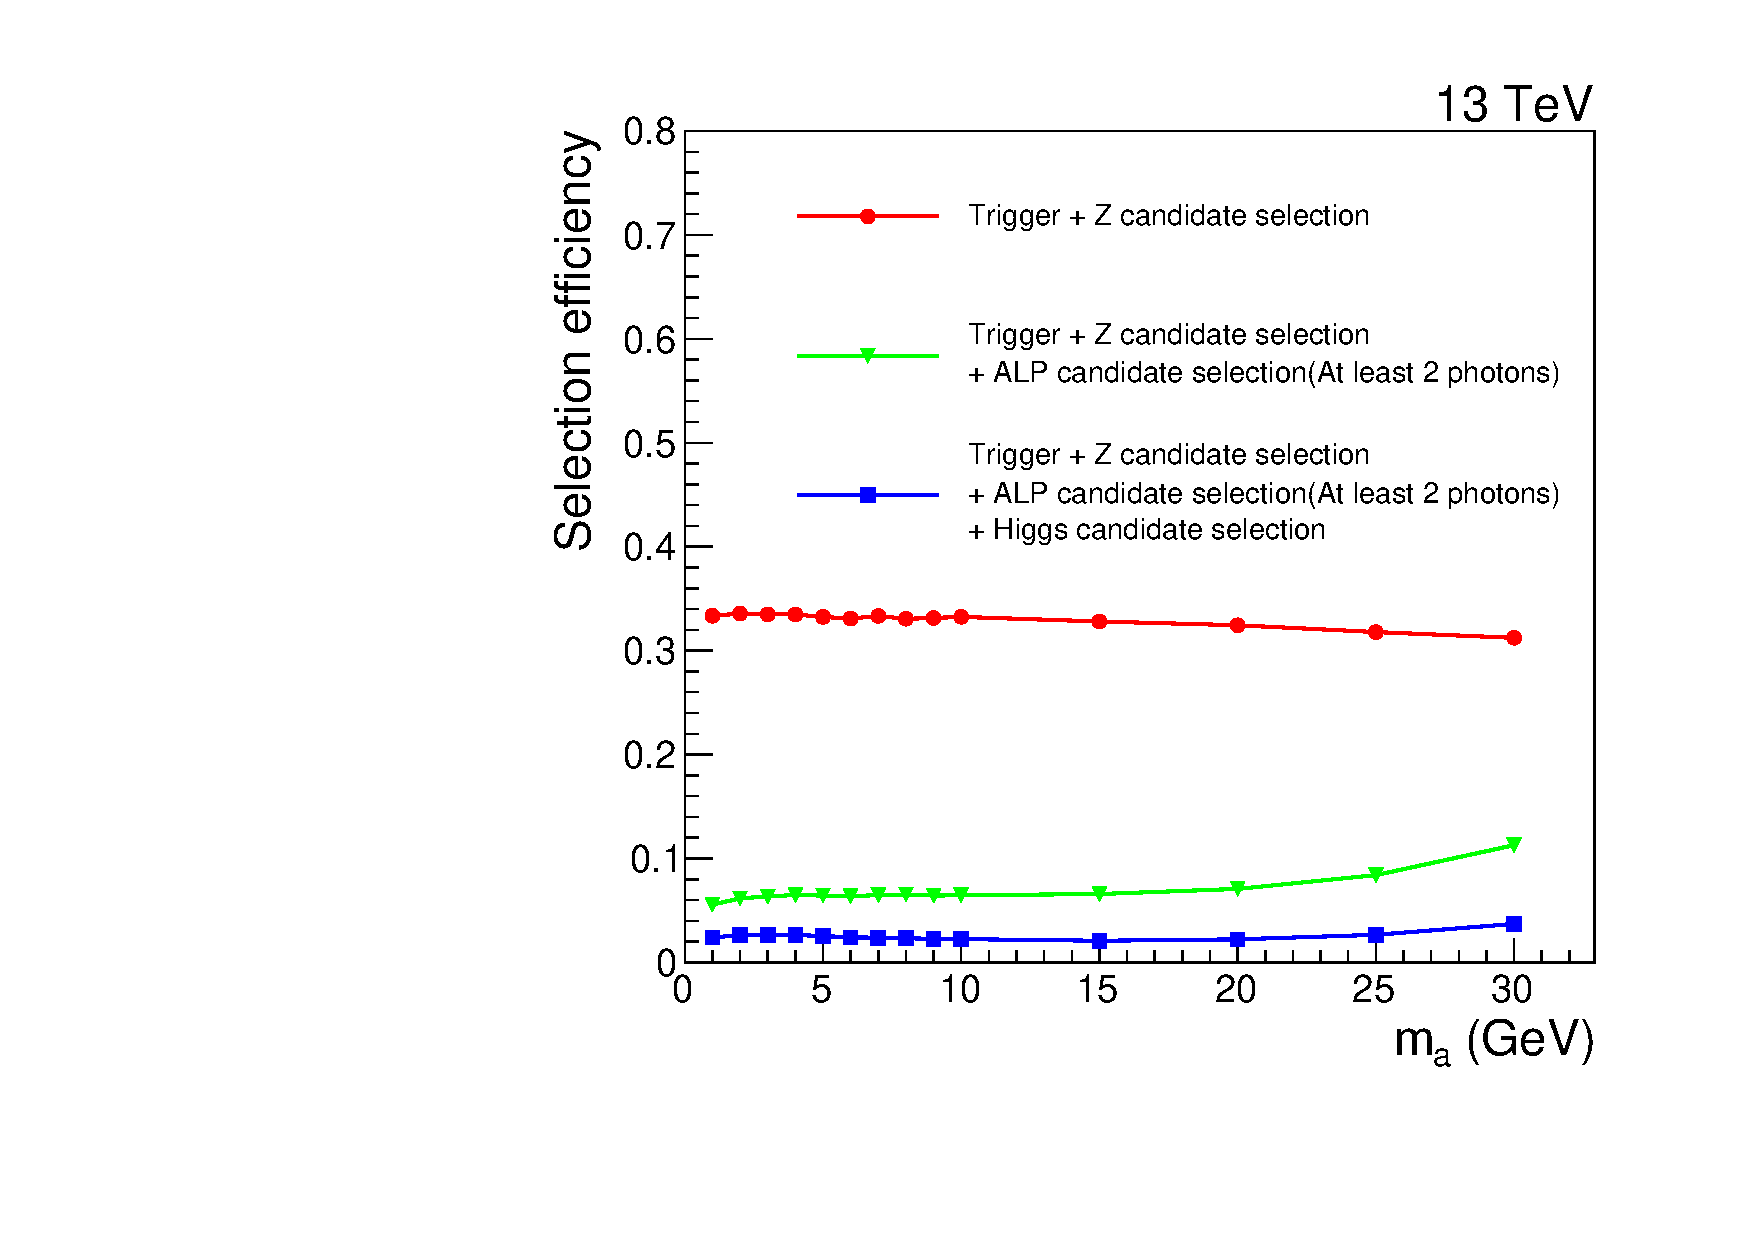
\includegraphics[width=0.42\textwidth]{figures/chapter04/cuteff_16.pdf}
    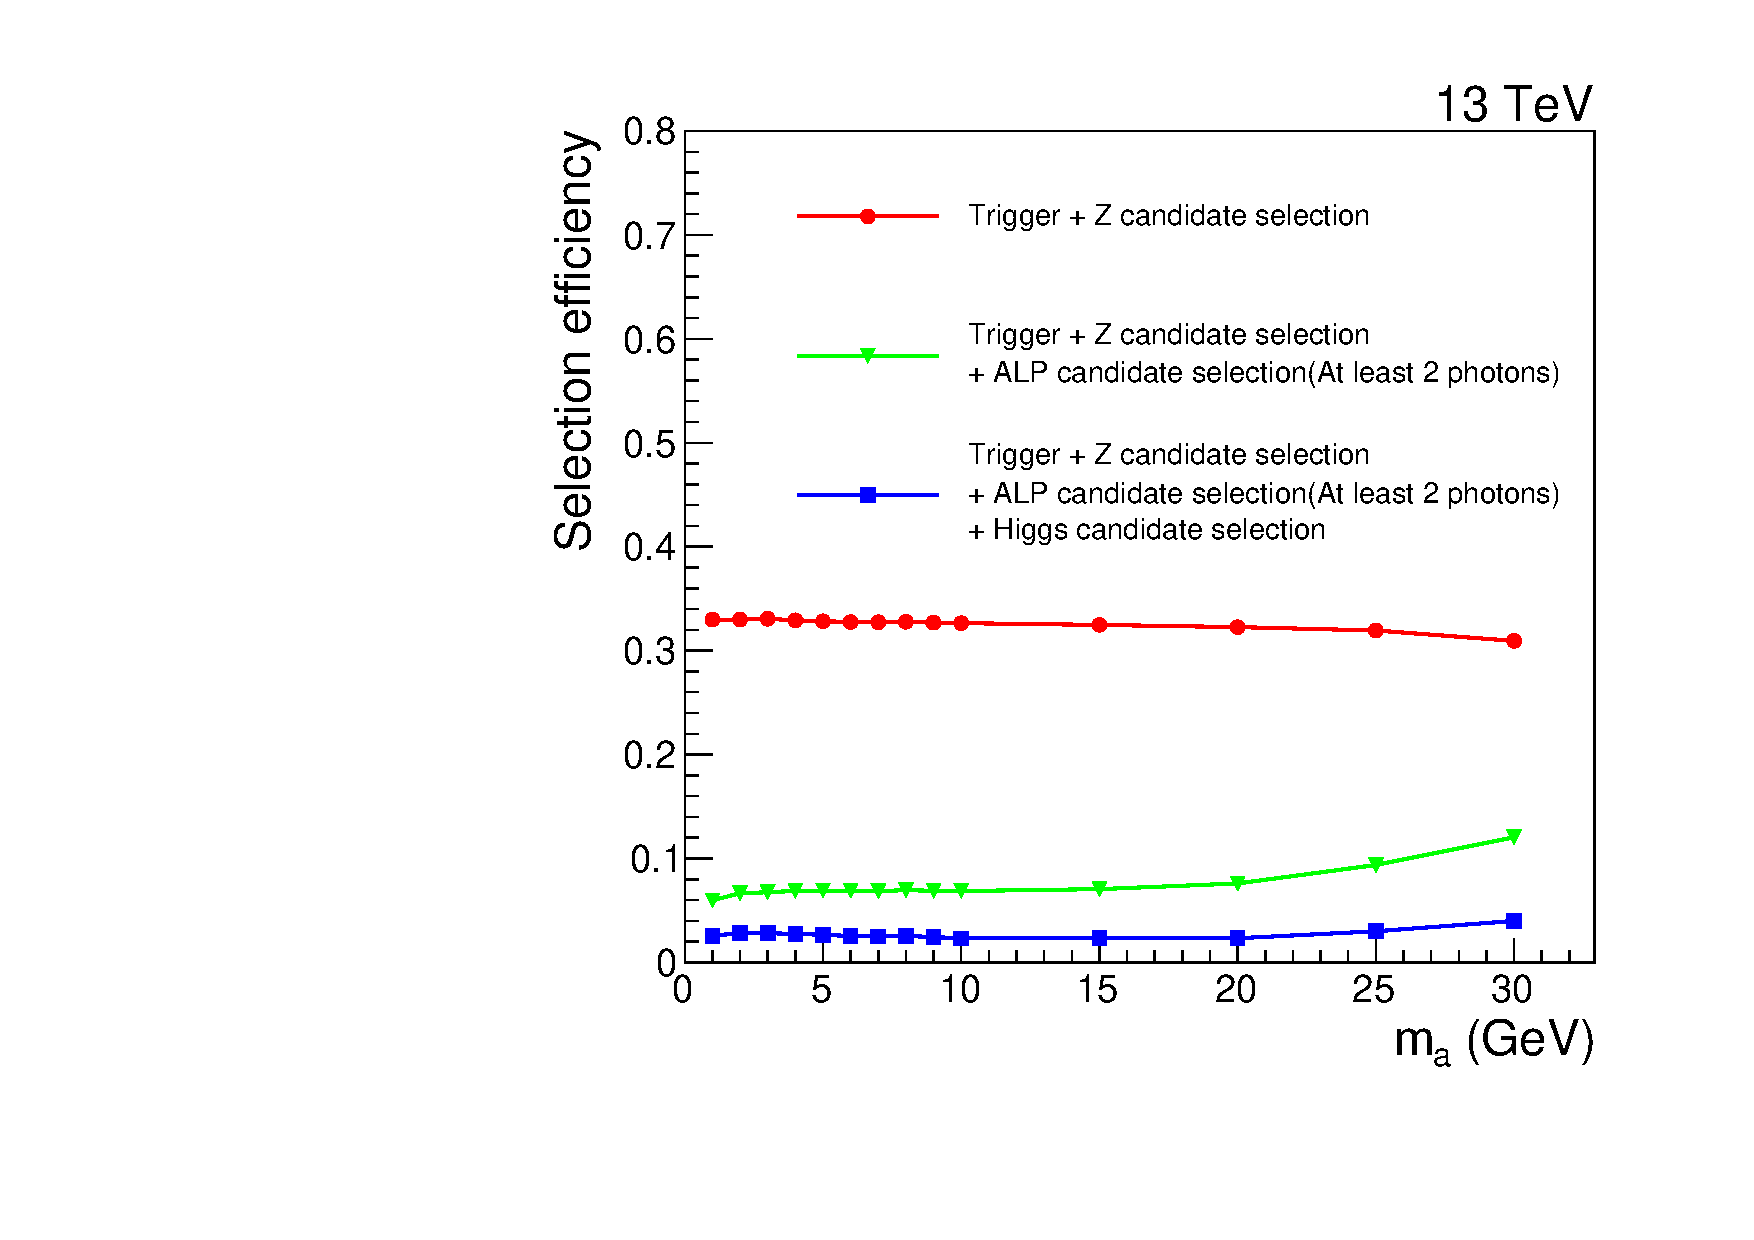
\includegraphics[width=0.42\textwidth]{figures/chapter04/cuteff_16APV.pdf} \\
		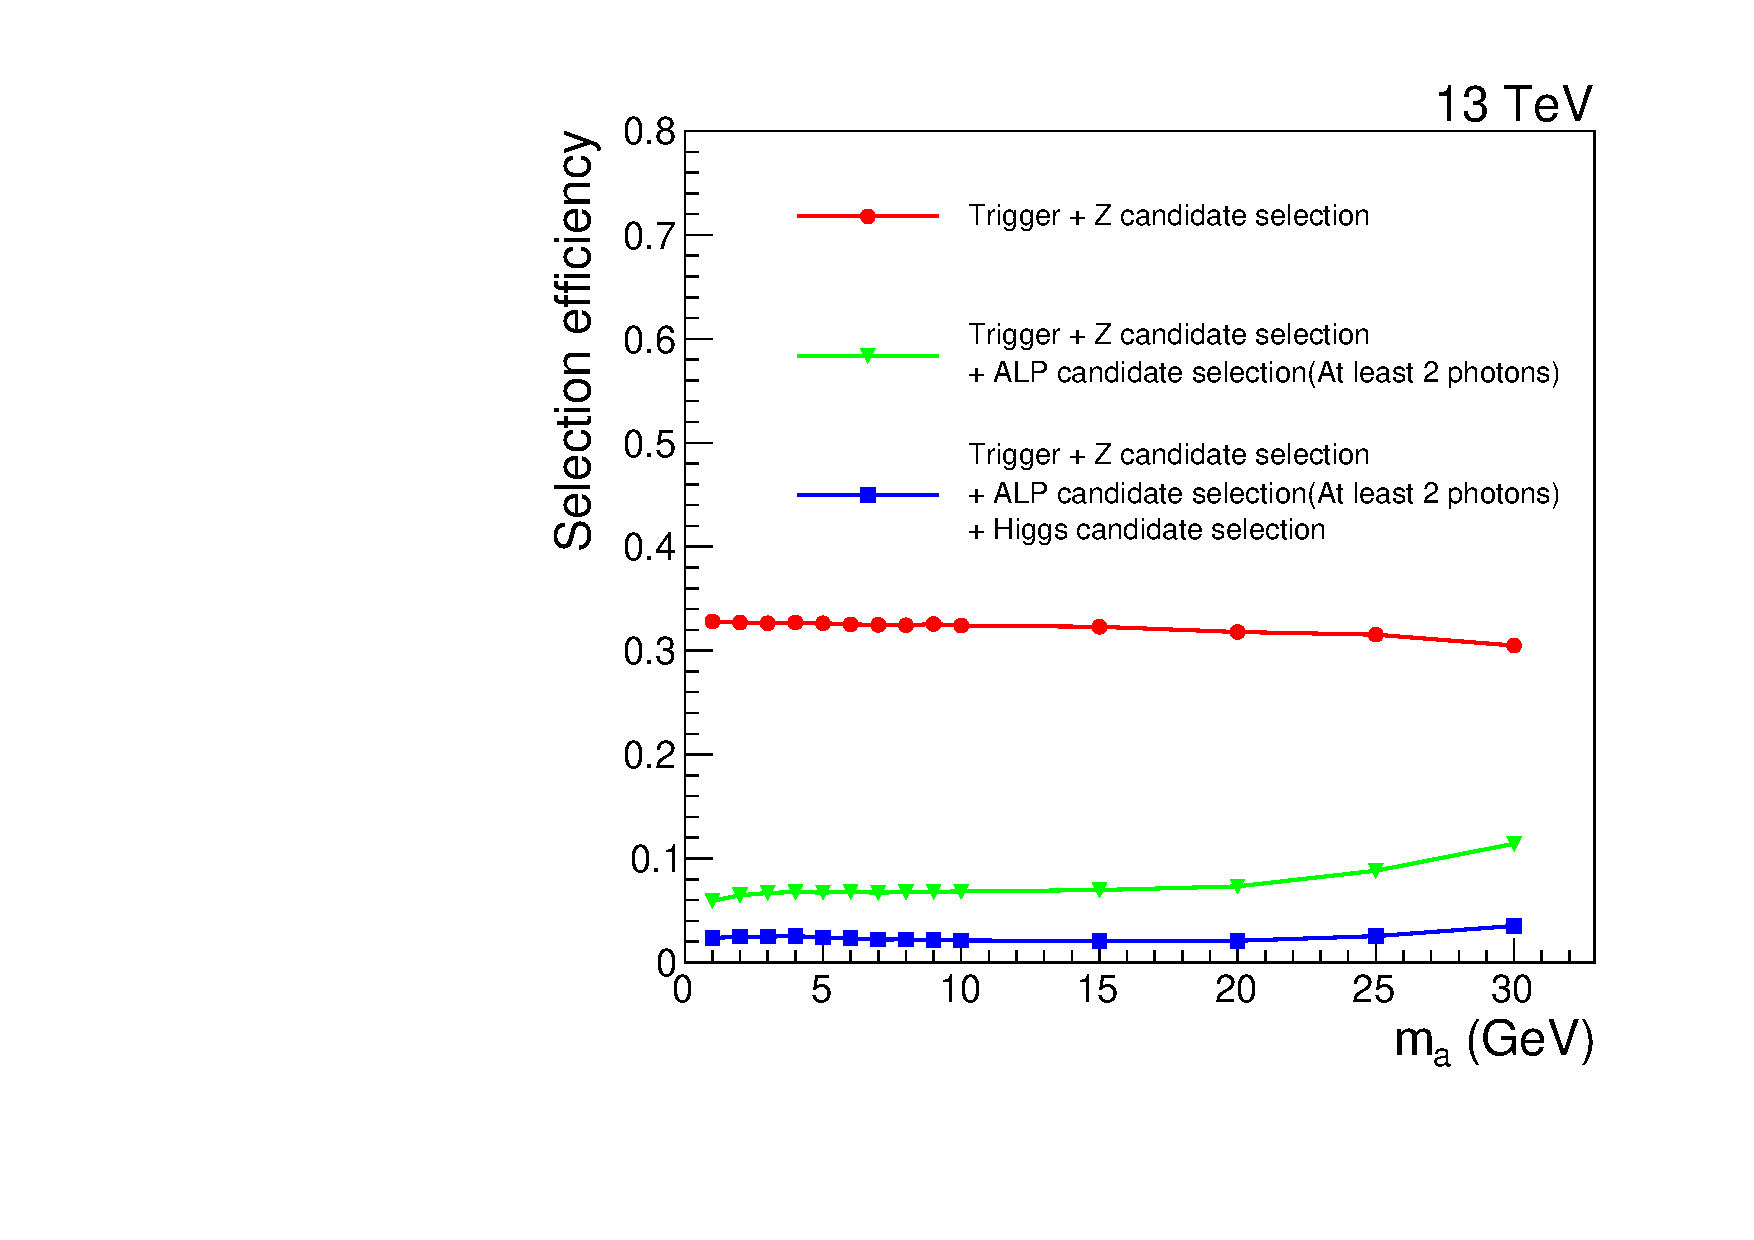
\includegraphics[width=0.42\textwidth]{figures/chapter04/cuteff_17.pdf}
		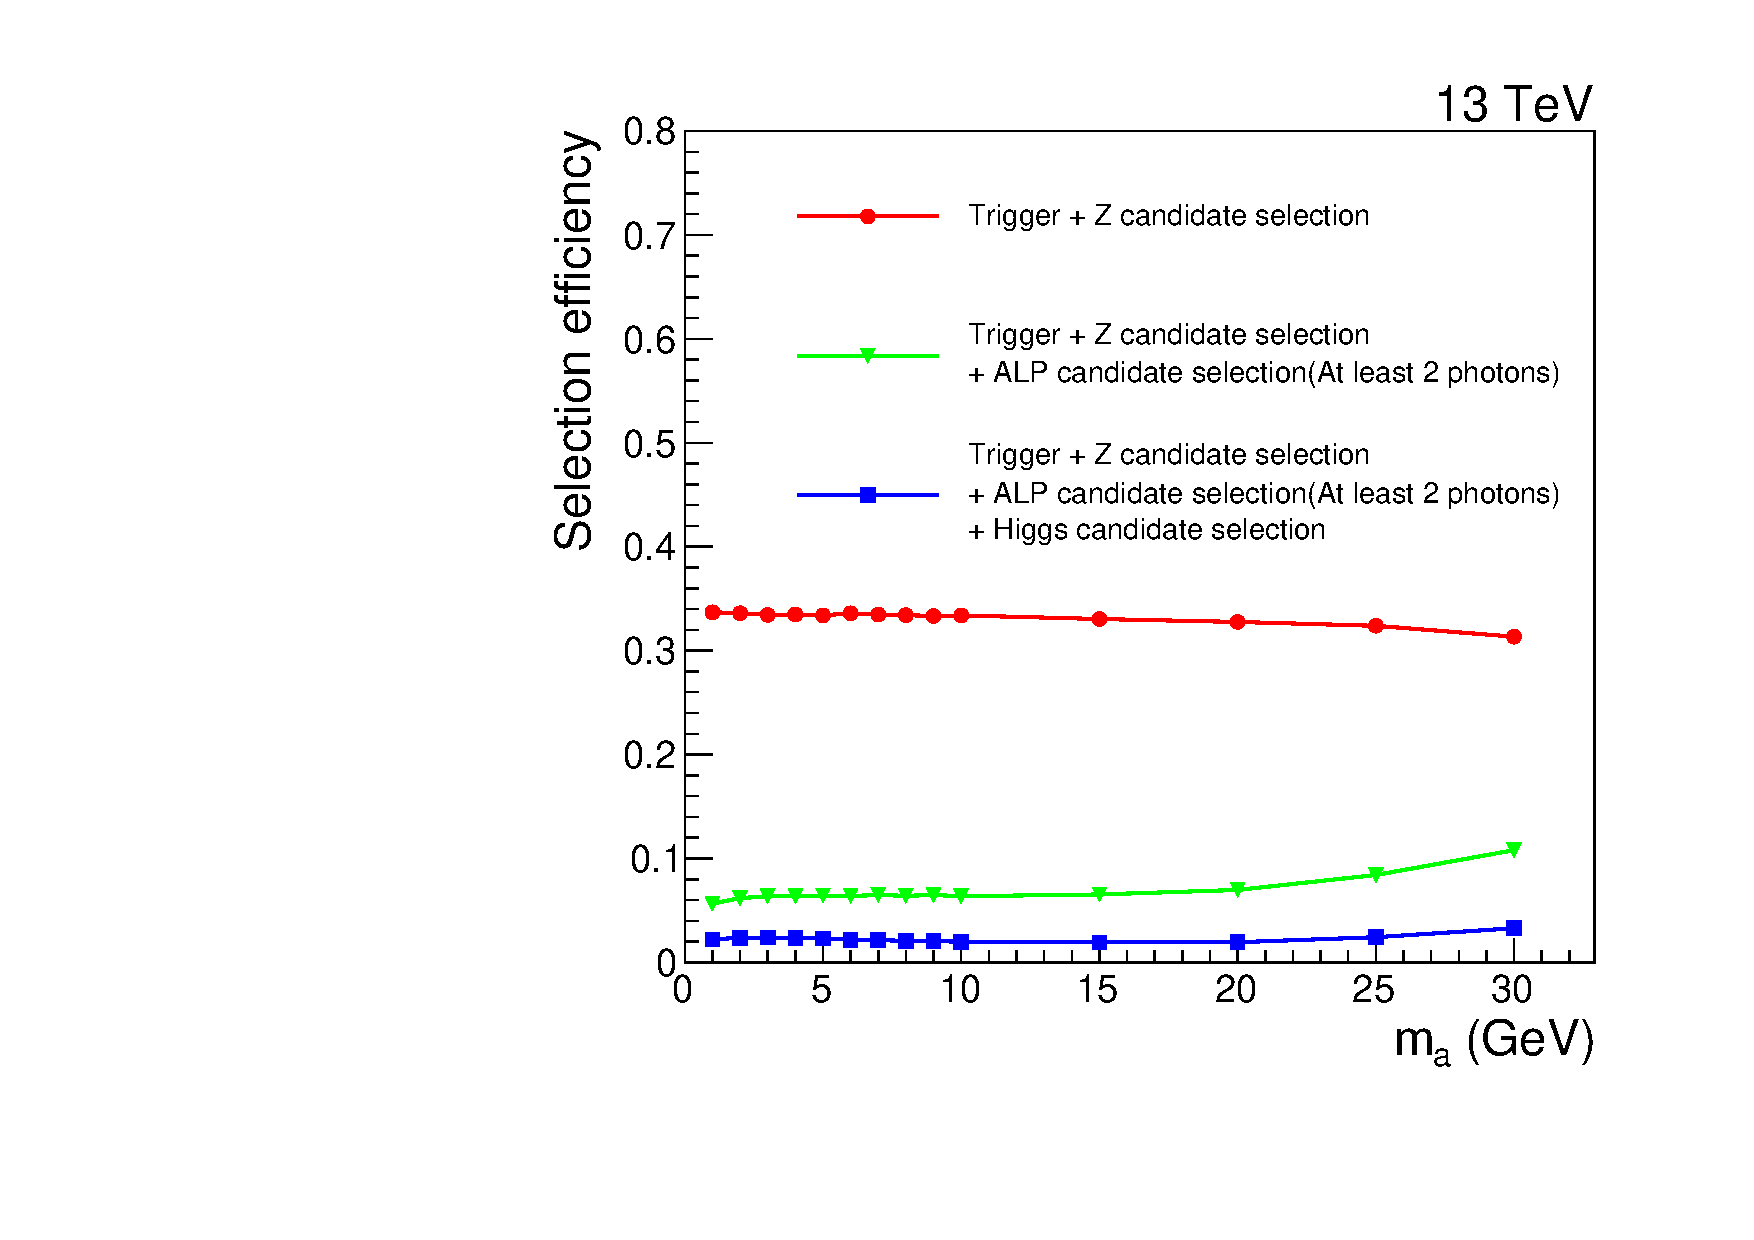
\includegraphics[width=0.42\textwidth]{figures/chapter04/cuteff_18.pdf}\\
    \bicaption{\quad \centering 信号事例的筛选效率,左上为2016年 post-VFP、右上为2016年 pre-VFP、左下为2017年、右下为2018年的结果}{\quad \centering The results of signal selection efficiency for 2016 post-VFP (top left), 2016 pre-VFP (top right), 2017 (bottom left), and 2018 (bottom right)}
    \label{fig:SelectionEff}
\end{center}
\end{figure}



\section{决策树法优化事例筛选}\label{sec:BDT}

为了进一步区分信号和本底,本分析采取了多变量分析(MVA)的策略,使用XGBoost软件包~\cite{XGBoost}中的提升决策树分类器来对信号和本底进行区分。此策略利用了已知类别的信号和本底事例,通过输入事例的变量信息来对提升决策树进行训练,得到能够区分信号和本底的最优模型。而后,将训练好的提升决策树模型应用于数据中,进而可以非常好的降低本底事例的影响,有效的提升信噪比。在本分析中,主要本底过程来自于标准模型Drell-Yan过程,因此,训练所使用的本底样本由Drell-Yan样本构成。

\begin{table}[h]
  \begin{center}
  \bicaption{\quad \centering 对提升决策树样本的处理}{\quad \centering Processes of BDTs samples}
    \scriptsize
    \begin{tabular}{lcc} \hline
        & Signal & Background \\ \hline
       Training & All mass points together (30\%) & $Z\rightarrow\ell\ell$ (60\%) \\ \hline
       Testing & All mass points together (20\%) & $Z\rightarrow\ell\ell$ (40\%) \\ \hline
       Application & All mass points together (50\%) & Data Driven \\
       (Signal modeling and limit evaluation) &  & \\ \hline
    \end{tabular}
    \label{tab:process}
  \end{center}
\end{table}

为了避免在对提升决策树进行训练、评估和应用的过程中产生关联,本分析将所有样本随机的分成了若干子样本,分别用于提升决策树的训练(Training)、评估(Testing)和应用(Application)。表格~\ref{tab:process}展示了用于训练、评估和应用的样本占总样本的比例。对于信号样本,所有质量点的样本都合并到了一起用于训练,应用样本仅仅用于信号模型的构建以及最终信号的提取。对于本底样本,由于最终的信号提取采取了数据驱动的方法,因此MC样本仅用于提升决策树的训练和评估。同时,为了增加训练过程中的样本统计量,本分析将三年的样本合并到一起用于训练。

\subsection{输入变量}

由于最终的信号提取是通过对$m_{\ell\ell\gamma\gamma}$的分布进行拟合所得到的,为了信号提取的方便,我们希望最终的本底分布是一个光滑平坦的分布。因此,本分析要求训练所使用的所有输入变量和$m_{\ell\ell\gamma\gamma}$之间不存在较强的关联性。本分析用于提升决策树训练所使用的输入变量定义如下:
\begin{itemize}
    \item 两个光子的横动量:$p_{T,\gamma1}$和$p_{T,\gamma2}$(其中,$\gamma1$和$\gamma2$分别表示横动量最大和次大的光子);
    \item 两个光子的$R_9$:$R_{9,\gamma1}$和$R_{9,\gamma2}$;
    \item 两个光子的$\sigma_{i\eta i\eta}$:$\sigma_{i\eta i\eta,\gamma1}$和$\sigma_{i\eta i\eta,\gamma2}$;
    \item 两个光子的PF光子隔离度:$I_{\gamma,\gamma1}$和$I_{\gamma,\gamma2}$;
    \item ALPs的PF光子隔离度$I_{\gamma,ALPs}$:对重建出的ALPs候选体周围半径$\dR<0.3$的锥形体内的所有PF光子横动量求和;
    \item 重建出的Z玻色子候选体和ALPs候选体之间的角距离:$\Delta R(Z,a)$;
    \item 两个光子之间的角距离:$\Delta R(\gamma1,\gamma2)$;
    \item 横动量最大的光子和Z玻色子候选体之间的角距离:$\Delta R (\gamma1,Z)$;
    \item 重建出的ALPs候选体横动量$\pt$和$m_{\ell\ell\gamma\gamma}$之间的比值:$p_{T,a}/m_{\ell\ell\gamma\gamma}$;
    \item 重建出的Higgs候选体横动量$p_{T,H}$;
\end{itemize}
对于这些变量的选择主要考虑了信号事例和本底事例中光子的动力学分布之间的差异、重建出的类轴子候选体和Z玻色子候选体、Higgs候选体之间的动力学分布之间的差异。由于在第~\ref{sec:EventReco}节中,轻子的选择已经要求了所有的轻子通过tight ID,因此和轻子相关的变量不再引入提升决策树的训练中。图~\ref{fig:BDT_Vars1}、~\ref{fig:BDT_Vars2}、~\ref{fig:BDT_Vars3}展示了这些输入变量的数据和蒙卡的分布情况,蒙卡样本被归一化到了数据所对应的积分亮度,图中所显示的系统误差主要包括了:光子效率误差、轻子效率误差以及堆积事例的影响。从这些分布中可以看到,数据和蒙卡之间的吻合程度非常好。此外,由于本底模型是通过数据驱动的方法直接从数据中拟合得到,数据和蒙卡之间个别微小的偏差并不会影响最终的结果。

\begin{figure}[htbp]
  \begin{center}
		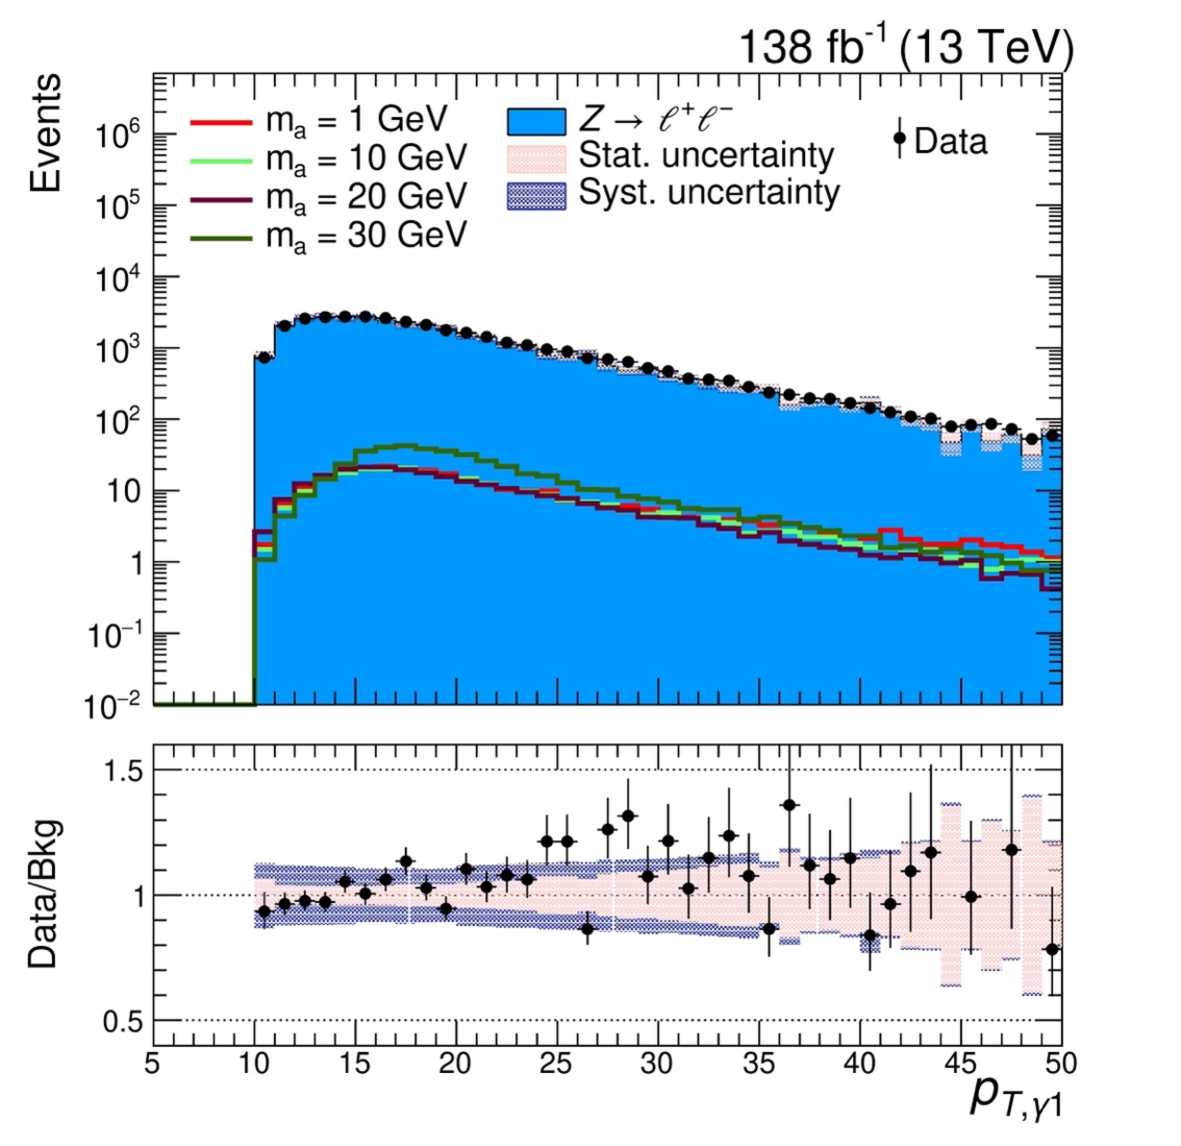
\includegraphics[width=0.42\textwidth]{figures/chapter04/BDT_input/pho1Pt_log.pdf}
    \includegraphics[width=0.42\textwidth]{figures/chapter04/BDT_input/pho2Pt_log.pdf} \\
		\includegraphics[width=0.42\textwidth]{figures/chapter04/BDT_input/pho1R9_log.pdf}
		\includegraphics[width=0.42\textwidth]{figures/chapter04/BDT_input/pho2R9_log.pdf}\\
		\includegraphics[width=0.42\textwidth]{figures/chapter04/BDT_input/pho1IetaIeta55_log.pdf}
		\includegraphics[width=0.42\textwidth]{figures/chapter04/BDT_input/pho2IetaIeta55_log.pdf}
    \bicaption{\quad \centering 输入变量$p_{T,\gamma1}$(左上)、$p_{T,\gamma2}$(右上)、$R_{9,\gamma1}$(左中)、$R_{9,\gamma2}$(右中)、$\sigma_{i\eta i\eta,\gamma1}$(左下)、$\sigma_{i\eta i\eta,\gamma2}$(右下)的数据和蒙卡的分布}{\quad \centering The data-MC distributions for the input variables: $p_{T,\gamma1}$ (top left), $p_{T,\gamma2}$ (top right), $R_{9,\gamma1}$ (middle left), $R_{9,\gamma2}$ (middle right), $\sigma_{i\eta i\eta,\gamma1}$ (bottom left), $\sigma_{i\eta i\eta,\gamma2}$ (bottom right)}
    \label{fig:BDT_Vars1}
\end{center}
\end{figure}

\begin{figure}[htbp]
  \begin{center}
		\includegraphics[width=0.42\textwidth]{figures/chapter04/BDT_input/pho1PIso_noCorr_log.pdf}
        \includegraphics[width=0.42\textwidth]{figures/chapter04/BDT_input/pho2PIso_noCorr_log.pdf} \\
		\includegraphics[width=0.42\textwidth]{figures/chapter04/BDT_input/ALP_calculatedPhotonIso_log.pdf}
		\includegraphics[width=0.42\textwidth]{figures/chapter04/BDT_input/var_dR_g1g2_log.pdf}\\
		\includegraphics[width=0.42\textwidth]{figures/chapter04/BDT_input/var_dR_Za_log.pdf}
		\includegraphics[width=0.42\textwidth]{figures/chapter04/BDT_input/var_dR_g1Z_log.pdf}\\
    \bicaption{\quad \centering 输入变量$I_{\gamma,\gamma1}$(左上)、$I_{\gamma,\gamma2}$(右上)、$I_{\gamma,ALPs}$(左中)、$\Delta R(\gamma1,\gamma1)$(右中)、$\Delta R(Z,a)$(左下)、$\Delta R (\gamma1,Z)$(右下)的数据和蒙卡的分布}{\quad \centering The data-MC distributions for the input variables: $I_{\gamma,\gamma1}$(top left), $I_{\gamma,\gamma2}$ (top right), $I_{\gamma,ALPs}$ (middle left), $\Delta R(\gamma1,\gamma1)$ (middle right), $\Delta R(Z,a)$ (bottom left), $\Delta R (\gamma1,Z)$ (bottom right)}
    \label{fig:BDT_Vars2}
\end{center}
\end{figure}

\begin{figure}[htbp]
  \begin{center}
		\includegraphics[width=0.42\textwidth]{figures/chapter04/BDT_input/var_PtaOverMh_log.pdf}
        \includegraphics[width=0.42\textwidth]{figures/chapter04/BDT_input/H_pt_log.pdf} \\
    \bicaption{\quad \centering 输入变量$p_{T,a}/m_{\ell\ell\gamma\gamma}$(左图)、$p_{T,H}$(右图)的数据和蒙卡的分布}{\quad \centering The data-MC distributions for the input variables: $p_{T,a}/m_{\ell\ell\gamma\gamma}$(left), $p_{T,H}$ (right)}
    \label{fig:BDT_Vars3}
\end{center}
\end{figure}

\begin{figure}[htbp]
  \begin{center}
		\includegraphics[width=0.6\textwidth]{figures/chapter04/BDT_input/param_log.pdf}
    \bicaption{\quad \centering 输入变量$(\ma-\mhyp)/\mllgg$的数据和蒙卡的分布}{\quad \centering The data-MC distributions for the input variable: $(\ma-\mhyp)/\mllgg$}
    \label{fig:BDT_Vars4}
\end{center}
\end{figure}

除了以上变量外,为了使得分类器的输出对整个$m_a$的范围都具有均匀且灵敏的性质,本分析使用了参数化的决策树林法~\cite{Baldi_2016}。在这个方法中,训练所使用的样本被参数化为$m_a$的函数,一个等于假设的类轴子质量的参数$\mhyp$被用作训练的输入变量,具体定义如下:
\begin{itemize}
    \item 重建出来的类轴子质量和假设的类轴子质量之间的差值和Higgs候选体质量的比值:$(\ma-\mhyp)/\mllgg$。
\end{itemize}
图~\ref{fig:BDT_Vars4}展示了这个参数的分布情况。当对模型进行训练的时候,信号样本的$\mhyp$被设置成对应样本的$\ma$的值,而本底样本的$\mhyp$均匀随机的分布在所有可能的14个$\ma$质量点之间。对于模型的评估和应用,数据和蒙卡样本中的参数$\mhyp$被设置成我们所希望寻找的$\ma$的值。比如,我们想要对5$\GeV$的类轴子进行寻找,数据和蒙卡样本中的参数$\mhyp$被固定为5,而后对提升决策树的输出进行筛选得到对应于5$\GeV$的数据和本底分布,并应用于最终的信号提取。


\subsection{模型训练}

在训练提升决策树的时候,所有的信号和本底样本都归一化到了整个Run2运行过程中的积分亮度。同时为了提高统计量,信号和本底三年的样本分别合并到一起用于训练。在提升决策树模型的构建中,本分析考虑了以下参数:
\begin{itemize}
    \item n\_estimators:决策树林的个数;
    \item max\_depth:每棵决策树的最大深度;
    \item learning\_rate:模型迭代时参数的更新步长;
    \item min\_child\_weight:最小子叶节点样本权重和,如果在此节点权重小于这个值,则停止分裂,从而有效的防止过拟合。
\end{itemize}

在训练的过程中,为了使得训练结果最优化,本分析在以上参数的参数空间进行了扫描训练,评判标准是验证样本集的接收者操作特征曲线下的面积(ROC AUC),这个参数可以用来评判模型训练的好坏,AUC的值越高表明模型训练的越好。其中,验证样本集是由训练样本集通过使用软件包scikit-learn~\cite{scikit-learn}中的交叉验证工具所得到的。为了找到具有最优性能的可能参数组合,本分析使用了GridSearchCV的方法~\cite{gridcv}。在此方法中,具有不同参数组合的提升决策树被用于训练并比较它们之间的性能差异,即AUC的值。在每一个参数格点上,提升决策树的训练使用了交叉验证的方法,主要步骤包括:
\begin{itemize}
    \item 将样本平均分为k部分;
    \item 将其中的k-1个部分用于训练模型,剩下的一个部分用于验证模型,并重复这个步骤遍历样本的所有部分。
\end{itemize}
而后交叉验证所得到的k个ROC AUC的值的平均值作为对应参数格点的AUC值。

本分析使用了k=2的交叉验证方法,对参数空间的格点扫描范围在列表~\ref{tab:BDT_para_scan}中展示。其中,AUC的值在所有参数组合形式中的变化小于0.3\%,这意味着训练出来的提升决策树具有非常好的稳定性。列表~\ref{tab:BDT_para_scan}也展示了最终用于分类所使用的参数组合。

训练过程中各个输入变量对模型的重要性(Importance)可以使用基尼指数(Gini index)错误率作为评价指标来衡量,其直观意义表示某一提升决策树节点中某一特征类别标记不一致的概率。某一特征在特定节点的重要性可以定义为该节点的基尼指数和分枝后的两个新节点的基尼指数之差,而后将所有节点的重要性相加并对所有特征进行归一化处理,可以得到训练过程中各个输入变量对模型的重要性,结果如图~\ref{fig:BDT_rank}所示。其中,重要性位于前四位的变量分别为$\sigma_{i\eta i\eta, \gamma 1}$、$(m_{a}-m_{a,hyp})/m_{\ell\ell\gamma\gamma}$、$\sigma_{i\eta i\eta, \gamma 2}$和$R_{9, \gamma 1}$,主要原因是本底过程中的假光子主要来自于将夸克和胶子产生的喷注错误的判断为光子,而相比于真正的光子,这些假光子在簇射过程中会在喷注中产生更多的次级粒子,从而使得喷注的$\sigma_{i\eta i\eta}$偏大、$R_9$偏小,因此这两个变量可以用来非常好的辨别真假光子。而对于变量$(m_{a}-m_{a,hyp})/m_{\ell\ell\gamma\gamma}$,由于其使用了双光子的不变质量信息,重建出的$m_a$主要分布在$\mhyp$附近,使得该变量对于信号样本只能集中分布在0附近,而对于本底样本,不同的动力学性质使得该变量可能位于偏离0的位置,因此具有非常好的信号本底识别度。

\begin{table}[h]
  \begin{center}
  \bicaption{\quad \centering 为寻找最优参数选项所执行的扫描列表以及用于最终分类的参数}{\quad \centering List of scans performed to look for the best parameters option, and the parameters used for the final categorization}
    \begin{tabular}{ccccc} \hline
       \multicolumn{4}{c} {Parameter Grid} & Option \\ \hline
       n\_estimators & max\_depth & learning\_rate & min\_child\_weight & AUC \\ \hline
       500 & 3 & 0.05 & 5 & $0.9878$\\
       1000 & 4 & 0.1 & & $\backsim$\\
       1500 & 5 & 0.15 & & $0.9907$\\ \hline
       \multicolumn{5}{c} {Parameter used for the categorization}\\ \hline 
       1500 & 3 & 0.15 & 5 & 0.9907 \\ \hline 
    \end{tabular}
    \label{tab:BDT_para_scan}
  \end{center}
\end{table}

\begin{figure}[htbp]
  \begin{center}
		\includegraphics[width=0.6\textwidth]{figures/chapter04/BDT_score/rank.png}
    \bicaption{\quad \centering 输入变量的重要性}{\quad \centering The importance of the input variables}
    \label{fig:BDT_rank}
\end{center}
\end{figure}

\subsection{模型评估}

训练样本和评估样本的提升决策树得分分布如图~\ref{fig:BDT_evalue}所示。其中,将评估样本集通过训练模型得到的信号和本底的分布与训练样本集的分布进行K-S检验可以得到对应的p值分别为0.96和0.23,这说明对提升决策树的训练是合理的,没有发生过拟合。通过将$\mhyp$设置为对应不同$\ma$的值,可以对不同ALPs质量点的提升决策树得分分别进行评估。因此,对于不同的ALPs质量点,可以分别得到不同的信号、数据和本底的提升决策树得分分布,如图~\ref{fig:BDT_score1}、~\ref{fig:BDT_score2}、~\ref{fig:BDT_score3}所示。

\begin{figure}[htbp]
  \begin{center}
		\includegraphics[width=0.52\textwidth]{figures/chapter04/BDT_score/BDT_output-2.png}
    \bicaption{\quad \centering 训练样本和评估样本的提升决策树得分分布}{\quad \centering Distributions of the BDTs score for training sample and testing sample}
    \label{fig:BDT_evalue}
\end{center}
\end{figure}

\begin{figure}[htbp]
  \begin{center}
		\includegraphics[width=0.42\textwidth]{figures/chapter04/BDT_score/mvaVal_M1_log.png}
        \includegraphics[width=0.42\textwidth]{figures/chapter04/BDT_score/mvaVal_M2_log.png} \\
		\includegraphics[width=0.42\textwidth]{figures/chapter04/BDT_score/mvaVal_M3_log.png}
		\includegraphics[width=0.42\textwidth]{figures/chapter04/BDT_score/mvaVal_M4_log.png}\\
		\includegraphics[width=0.42\textwidth]{figures/chapter04/BDT_score/mvaVal_M5_log.png}
		\includegraphics[width=0.42\textwidth]{figures/chapter04/BDT_score/mvaVal_M6_log.png}\\
    \bicaption{\quad \centering 不同ALPs质量点下的提升决策树得分分布}{\quad \centering Distributions of the BDTs score for different ALPs mass points}
    \label{fig:BDT_score1}
\end{center}
\end{figure}

\begin{figure}[htbp]
  \begin{center}
		\includegraphics[width=0.42\textwidth]{figures/chapter04/BDT_score/mvaVal_M7_log.png}
        \includegraphics[width=0.42\textwidth]{figures/chapter04/BDT_score/mvaVal_M8_log.png} \\
		\includegraphics[width=0.42\textwidth]{figures/chapter04/BDT_score/mvaVal_M9_log.png}
		\includegraphics[width=0.42\textwidth]{figures/chapter04/BDT_score/mvaVal_M10_log.png}\\
		\includegraphics[width=0.42\textwidth]{figures/chapter04/BDT_score/mvaVal_M15_log.png}
		\includegraphics[width=0.42\textwidth]{figures/chapter04/BDT_score/mvaVal_M20_log.png}\\
    \bicaption{\quad \centering 不同ALPs质量点下的提升决策树得分分布}{\quad \centering Distributions of the BDTs score for different ALPs mass points}
    \label{fig:BDT_score2}
\end{center}
\end{figure}

\begin{figure}[htbp]
  \begin{center}
		\includegraphics[width=0.42\textwidth]{figures/chapter04/BDT_score/mvaVal_M25_log.png}
        \includegraphics[width=0.42\textwidth]{figures/chapter04/BDT_score/mvaVal_M30_log.png} \\
    \bicaption{\quad \centering 不同ALPs质量点下的提升决策树得分分布}{\quad \centering Distributions of the BDTs score for different ALPs mass points}
    \label{fig:BDT_score3}
\end{center}
\end{figure}

\subsection{事例分类}

为了能够得到最高的信号显著度,本分析根据提升决策树的输出得分将所有事例分为了不同的类别,具体评判标准为使得近似平均显著度~\cite{Cowan:2010js}(Approximate Mean Significance,AMS)具有极大值。AMS的定义为:
\begin{equation}
    \textrm{AMS} = \sqrt{2((S+B)\ln{(1+\frac{S}{B})} - S)}\label{con:AMS}.
\end{equation}
其中,S和B分别表示信号区间(Signal region,SR)的信号和本底事例数,信号区间的定义为$115 <\mllgg< 135\GeV$。对于固定类别数量的分类情况,提升决策树的筛选边界条件被选为使得每个类别的AMS平方和开根号具有极大值的得分。此外,由于最终信号的提取是通过利用参数化的函数形式对数据中的$\mllgg$分布进行拟合所得到的。其中,描述本底分布的本底模型是通过利用多种解析函数对数据中的$\mllgg$本底分布进行拟合所得到的。因此,在分类的过程中使得最终通过提升决策树筛选的数据具有足够的统计量对本底模型的构建具有至关重要的作用。为了满足这一条件,对提升决策树筛选边界的优化过程中同时要求了每个类别中的边带区(side-band region,SB)至少含有8个通过提升决策树筛选边界的本底事例,其中边带区定义为$95 <\mllgg< 115\GeV$和$135 <\mllgg< 180\GeV$。

由于不同类轴子质量下的提升决策树分数分布不同,因此这个分类步骤是针对不同的类轴子质量点进行的。在优化的过程中,方程~\ref{con:AMS}中B的计算使用了本底蒙卡的提升决策树得分在信号区间的分布直方图。直方图的bin越精细,求得的AMS越准确,但与之带来的是每个bin中的统计涨落会增大。因此,为了在优化的过程中降低统计涨落的影响,本分析将本底蒙卡分布进行了平滑化,并将平滑化后的分布用于AMS的计算,平滑化的过程使用的是TGraphSmooth中的SmoothSuper方法。同时,为了使平滑过程以最佳的方式处理提升决策树得分的分布形状,平滑过程去除了提升决策树得分小于0.1的事例。图~\ref{fig:bkg_smooth1}、~\ref{fig:bkg_smooth2}、~\ref{fig:bkg_smooth3}展示了不同ALPs质量点信号区间内的本底提升决策树得分分布。其中,黑色直方图表示平滑之前的本底分布,红色曲线表示平滑之后的分布,绿色和蓝色曲线分别表示平滑过程考虑了$\pm1\sigma$的误差之后的分布形状。

\begin{figure}[htbp]
  \begin{center}
		\includegraphics[width=0.42\textwidth]{figures/chapter04/bkg_smooth/M1_all_DYJetsToLL_SR.png}
        \includegraphics[width=0.42\textwidth]{figures/chapter04/bkg_smooth/M2_all_DYJetsToLL_SR.png} \\
		\includegraphics[width=0.42\textwidth]{figures/chapter04/bkg_smooth/M3_all_DYJetsToLL_SR.png}
		\includegraphics[width=0.42\textwidth]{figures/chapter04/bkg_smooth/M4_all_DYJetsToLL_SR.png}\\
		\includegraphics[width=0.42\textwidth]{figures/chapter04/bkg_smooth/M5_all_DYJetsToLL_SR.png}
		\includegraphics[width=0.42\textwidth]{figures/chapter04/bkg_smooth/M6_all_DYJetsToLL_SR.png}\\
    \bicaption{\quad \centering 信号区间内的本底提升决策树得分分布,红色曲线表示平滑之后的分布}{\quad \centering Distributions of the BDTs score for background in the signal region are shown. The result of performing a smoothing is also shown in red}
    \label{fig:bkg_smooth1}
\end{center}
\end{figure}

\begin{figure}[htbp]
  \begin{center}
		\includegraphics[width=0.42\textwidth]{figures/chapter04/bkg_smooth/M7_all_DYJetsToLL_SR.png}
        \includegraphics[width=0.42\textwidth]{figures/chapter04/bkg_smooth/M8_all_DYJetsToLL_SR.png} \\
		\includegraphics[width=0.42\textwidth]{figures/chapter04/bkg_smooth/M9_all_DYJetsToLL_SR.png}
		\includegraphics[width=0.42\textwidth]{figures/chapter04/bkg_smooth/M10_all_DYJetsToLL_SR.png}\\
		\includegraphics[width=0.42\textwidth]{figures/chapter04/bkg_smooth/M15_all_DYJetsToLL_SR.png}
		\includegraphics[width=0.42\textwidth]{figures/chapter04/bkg_smooth/M20_all_DYJetsToLL_SR.png}\\
    \bicaption{\quad \centering 信号区间内的本底提升决策树得分分布,红色曲线表示平滑之后的分布}{\quad \centering Distributions of the BDTs score for background in the signal region are shown. The result of performing a smoothing is also shown in red}
    \label{fig:bkg_smooth2}
\end{center}
\end{figure}

\begin{figure}[htbp]
  \begin{center}
		\includegraphics[width=0.42\textwidth]{figures/chapter04/bkg_smooth/M25_all_DYJetsToLL_SR.png}
        \includegraphics[width=0.42\textwidth]{figures/chapter04/bkg_smooth/M30_all_DYJetsToLL_SR.png} \\
    \bicaption{\quad \centering 信号区间内的本底提升决策树得分分布,红色曲线表示平滑之后的分布}{\quad \centering Distributions of the BDTs score for background in the signal region are shown. The result of performing a smoothing is also shown in red}
    \label{fig:bkg_smooth3}
\end{center}
\end{figure}

本分析考虑了类别的个数分别为1和2的情况,经比较发现,对于所有ALPs的质量点,类别个数为2的信号显著度相比于类别个数为1的显著度增加小于1\%。因此,对于最终的提升决策树分类,本分析只考虑了一个类别的情况,针对每个质量点选择一个提升决策树最优得分阈值,所有小于这个阈值的事例被去除掉,只有通过这个阈值的事例被用于最终的信号提取。表格~\ref{tab:boundary}详细说明了提升决策树的筛选边界、相关信号效率和本底事例数。

\begin{table}[h]
    \small
    \begin{center}
    \bicaption{\quad \centering 用于定义分析类别的最小提升决策树输出值以及相关的信号效率和本底事例数}{\quad \centering Minimum BDTs output values used to define the analysis categories, with the associated signal efficiencies and background yields}
      \begin{tabular}{cccc} 
        $\ma$ (\GeV) & Min. BDT & Signal efficiency & Drell--Yan\\ 
        & output value &  & background yields \\ \hline
       1 & 0.955 & $49 \pm 3.3\%$ & $83 \pm 27$\\
       2 & 0.980 & $67 \pm 2.7\%$ & $26 \pm 10$\\
       3 & 0.985 & $76 \pm 2.4\%$ & $7.9 \pm 4.9$\\
       4 & 0.980 & $84 \pm 2.1\%$ & $5.1 \pm 4.5$\\
       5 & 0.985 & $85 \pm 2.1\%$ & $5.1 \pm 3.9$\\
       6 & 0.990 & $82 \pm 2.3\%$ & $2.5 \pm 2.2$\\
       7 & 0.985 & $86 \pm 2.1\%$ & $5.3 \pm 4.0$\\
       8 & 0.990 & $80 \pm 2.5\%$ & $11 \pm 4.8$\\
       9 & 0.990 & $78 \pm 2.5\%$ & $16 \pm 5.6$\\
       10 & 0.990 & $77 \pm 2.6\%$ & $11 \pm 4.7$\\ 
       15 & 0.990 & $70 \pm 2.9\%$ & $13 \pm 5.2$\\
       20 & 0.990 & $63 \pm 3.1\%$ & $18 \pm 6.1$\\
       25 & 0.985 & $64 \pm 2.7\%$ & $37 \pm 11$\\
       30 & 0.980 & $67 \pm 2.2\%$ & $44 \pm 13$\\  
      \end{tabular}
      \label{tab:boundary}
    \end{center}
\end{table}

\section{用于信号提取的统计原理}\label{sec:Fit}

本分析采取了对数据中的$\mllgg$的分布使用联合unbinned极大似然拟合的方法来对信号进行提取并给出截面上限的测量结果~\cite{likelihoodRatio},结果展示了$1<\ma<30\GeV$并且以1$\GeV$为步长范围内的截面上限。似然函数的定义使用了用于描述信号和本底$\mllgg$分布的解析函数模型,也包括了第~\ref{sec:Sys}节用于描述实验和理论系统误差的冗余参数。我们所感兴趣的参数(Parameters Of Interest,POI)的最优拟合值和置信区间可以通过利用轮廓似然检验统计量(Profile likelihood test statistic)进行估计,其定义为:
\begin{equation}\label{eq:4-02}
    \lambda(\vec{\alpha})=-2 \ln \left(\frac{L(\vec{\alpha}, \hat{\vec{\theta}}_{\vec{\alpha}})}{L(\hat{\vec{\alpha}}, \hat{\vec{\theta}})}\right)
\end{equation}
其中,$\hat{\vec{\alpha}}$和$\hat{\vec{\theta}}$描述了对POI和冗余参数的无条件极大似然估计值,而$\hat{\vec{\theta}}_{\vec{\alpha}}$表示固定POI的值为$\vec{\alpha}$的条件下冗余参数的极大似然值。在利用函数~\ref{eq:4-02}对$\mllgg$分布的拟合中,取似然比对数的两倍负值的极小值作为对应POI的估计值。在本分析中,POI对应的就是信号强度,定义为测量的截面和预计截面的比值。

\section{本底建模}\label{sec:Bkg}

本分析中本底的估计是通过对数据中的$\mllgg$不变质量谱直接进行参数拟合所得到的。这一节中,我们将详细介绍本底估计的步骤,包括使用参数化的解析函数对数据中$95<\mllgg<180\GeV$的范围直接进行拟合以及对本底模型偏差的考虑。拟合范围包括了由光子$\pt$筛选所造成的在110$\GeV$附近的turn-on。

\subsection{本底模型}

用于本底拟合的本底概率分布函数(Probability Distribution Function,PDF)由一个用于描述turn-on部分的高斯函数和一个下降谱与阶梯函数的乘积之间的卷积所构成。阶梯函数的作用是在质量谱上定义一个截断点,在这个截断点以下的数据点不受下降谱的影响而仅由用于描述turn-on的高斯函数来描述。如果将高斯函数部分标记为$\mathcal{N}$,下降谱定义为$f$,阶梯函数定义为$\Theta$,用于本底拟合的PDF的通用形式可以表示为:
\begin{equation}\label{eq:4-03}
  \mathcal{F}(\mllgg;\mu,\sigma,s,\vec{\alpha}) := \int\mathcal{N}(\mu,\sigma)(\mllgg-t)f(t;\vec{\alpha})\Theta(s,t)dt,
\end{equation}
其中,$\mu$和$\sigma$表示高斯函数的参数;$s$表示阶梯函数的位置;$\vec{\alpha}$表示下降谱$f$所包含的参数集合。因此,本底拟合函数中的总参数量等于下降谱中的参数个数再加3。

由于对下降谱$f$的具体函数形式没有先验的信息,因此本分析中对本底的拟合采用了多种函数形式,包括Bernstein polynomials、Exponential series、Power law series和Laurent series,函数的具体定义如下:
\begin{itemize}
  \item N个指数函数的求和
    \begin{equation}
    NExp(m_{a}) := \sum_{i=1}^{N} f_{i}e^{p_{i}m_{a}}
    \end{equation}
    其中包含2N个参数:$p_{i} < 0$和$f_{i}$。最低阶的函数形式中$N = 1$,只含有一项。下一阶含有两个指数函数项,三个自由参数,因此在本分析中标记为exp3。
  \item N阶多项式的求和
    \begin{equation}
    NPow(m_{a}) := \sum_{i=1}^{N} f_{i}m_{a}^{p_{i}}
    \end{equation}
    一共含有2N个参数:$p_{i} < 0$和$f_{i}$。最低阶的函数形式中$N = 1$,只含有一项。
  \item N阶的Bernstein polynomials函数
    \begin{equation}
      \begin{split}
        Bern_{N}(\mllgg) &:= \sum_{i=0}^{N} f_{i}b_{i,N}(\mllgg)\\
        b_{i,N}(\mllgg) &:= {N \choose i} \mllgg^{i}(1-\mllgg^{N-i})
      \end{split}
    \end{equation}
    一共含有N个参数$f_{i}$。最低阶的函数形式中$N = 1$,只含有一项。
  \item N = 2、3或者4的Laurent series:
    \begin{equation}
      \begin{split}
      Lau_{2}(\mllgg) &:= f_{2}\mllgg^{-4} + f_{3}\mllgg^{-5}\\
      Lau_{3}(\mllgg) &:= f_{1}\mllgg^{-3} + f_{2}\mllgg^{-4} + f_{3}\mllgg^{-5}\\
      Lau_{4}(\mllgg) &:= f_{1}\mllgg^{-3} + f_{2}\mllgg^{-4} + f_{3}\mllgg^{-5} + f_{4}\mllgg^{-6}
      \end{split}
    \end{equation}
\end{itemize}

\subsection{包络线法}\label{sec:envelop_method}

在每个质量点,对于用于本底建模的下降谱的函数形式的选择具有一定的任意性。原则上来说,对本底PDF的选择可以作为测量过程中的系统误差,而该系统误差可以使用包络线~\cite{DiscreteProfilingMethod}(Envelope)法来评估。在这个方法中,不同PDF的选择作为整体似然函数中的一个离散的冗余参数,所有合理的函数形式都被考虑到包络线中。除此之外,同一个函数形式中的不同阶函数也被考虑了进来。每个类别中包络线的确切组成基于一组选择要求,这些要求考虑了拟合优度、F检验和偏差评估,详细选择步骤将会在第~\ref{sec:envelope_selection}节中进行介绍。

当对本底进行拟合的时候,包络线内所有的函数形式都被用来进行拟合。当对POI进行拟合的时候,具有最小$-2\ln{L}$的PDF被用于POI的测量。在这个过程中,似然函数是POI的一个函数,对于不同的POI的值,拟合最优的PDF不同。因此,包络线法考虑了不同POI值和不同最优拟合函数条件下的全局最优拟合函数。与此同时,包络线法会得到一个轮廓似然曲线,这个曲线比使用任何单独函数拟合得到的似然曲线都要更宽,这是因为包络线法的轮廓似然曲线考虑了所有单独函数的似然曲线,并且只截取所有曲线中似然值最小的部分。由此得到的似然曲线表明引入对PDF选择的不确定性会增加最终测量所得到的误差。

\subsection{包络选择}\label{sec:envelope_selection}

根据一系列的筛选条件,可以将一个个的单独函数添加到包络线中,这些筛选条件主要包括以下三个因素:拟合优度、F检验和偏差评估。

首先,最简单的要求是基于对拟合优度进行的筛选。对于本底拟合中所考虑的所有函数,计算对应的$\chi^{2}/DOF$值,其中DOF表示拟合的自由度个数。而后,得到$\chi^{2}/DOF$对应的p值。如果p值大于0.01,就认为这个函数通过了拟合优度的筛选,并且将其添加到包络线中。丢掉任何不满足这个条件的函数,因为这些函数不能够很好的描述数据中本底的分布。

第二个要考虑的因素是F检验的结果~\cite{Khachatryan:2014ira}。F检验是一种对下降谱的部分中具有同一函数形式、不同阶函数之间的选择的方法,这种方法比较了同一种函数形式中的低阶函数和高阶函数之间拟合结果。通常情况下,高阶函数往往可以给出更好的拟合结果。但是,它并不一定在统计显著度上给出更好的结果。如果使用高阶函数并没有明显的显著度提升,那么就可以使用低阶的函数形式达到类似的显著度,同时又不用引入过多的拟合参数。F检验的详细步骤如下:
\begin{itemize}
    \item 首先,对于指定的函数形式,选择阶数最低的函数对数据进行拟合。
    \item 然后,选择阶数第二低的函数并对同样的数据进行拟合。
    \item 两次拟合之间的似然函数差值$2\Delta NLL_{N+1}$用来决定是否更高阶的函数可以更好的描述数据中的本底。其中,变量$2\Delta NLL_{N+1}$满足自由度为M的$\chi^{2}$分布,M表示N+1阶函数和N阶函数之间的自由参数个数的差值。因此,可以求得$2\Delta NLL_{N+1}$对应的p值:
    \begin{equation}
    p-value = p(2\Delta NLL > 2\Delta NLL_{N+1}|\chi^{2}(M))
    \end{equation}
    \item 如果p值小于0.05,则认为更高阶的函数可以更好的描述数据中的本底。然后重复上述步骤来对下一阶的函数进行检验。相反的,如果p值大于0.05,则认为更高阶的函数用于描述数据中的本底时参数过多,此时终止F检验,表示用于描述数据的最高阶函数已经被找到。
\end{itemize}
可以将以上步骤用于所有函数形式中对最高阶函数的寻找。本分析考虑了每个函数形式中阶数最高为5的情况,并将所有函数形式中p值低于0.05的最高阶函数添加到包络线中用于最终的信号提取。除此之外,本分析同样将所有函数形式中通过第一个拟合优度筛选条件的低阶函数添加到包络线中。

选择包络线内的函数形式最后要考虑的因素是偏差评估。在通过拟合优度和F检验的筛选构成最初的包络线后,通过偏差评估来对包络线内的函数进行筛选,偏差评估的详细步骤会在第~\ref{sec:BiasStudy}节进行介绍。简单来说,针对包络线内的所有PDF产生相应的伪数据(Toys),然后利用包络线对产生的toys进行拟合,拟合结果可以用来计算信号显著度的偏差。如果偏差在可以接受的范围内,则将此包络线用于最终的信号提取。反之,如果包络线产生的偏差过大,我们可以考虑修改包络线的函数成分来降低偏差。通常情况下,可以通过使用被F检验所丢弃的更高阶的函数或者将对应偏差较大的函数形式从包络线中去除来降低包络线的偏差。使用这些参数更多的高阶函数往往可以很好的降低包络线的偏差。

图~\ref{fig:bkg_fTest1}、~\ref{fig:bkg_fTest2}、~\ref{fig:bkg_fTest3}展示了所有质量点的本底拟合所选择的包络线拟合函数形式,表格~\ref{tab:bkg_true}中汇总了最终用于信号提取的包络线函数形式。

\begin{figure}[htbp]
  \begin{center}
		\includegraphics[width=0.42\textwidth]{figures/chapter04/bkg_fTest/allPdfs_cat0_1.png}
        \includegraphics[width=0.42\textwidth]{figures/chapter04/bkg_fTest/allPdfs_cat0_2.png} \\
		\includegraphics[width=0.42\textwidth]{figures/chapter04/bkg_fTest/allPdfs_cat0_3.png}
		\includegraphics[width=0.42\textwidth]{figures/chapter04/bkg_fTest/allPdfs_cat0_4.png}\\
		\includegraphics[width=0.42\textwidth]{figures/chapter04/bkg_fTest/allPdfs_cat0_5.png}
		\includegraphics[width=0.42\textwidth]{figures/chapter04/bkg_fTest/allPdfs_cat0_6.png}\\
    \bicaption{\quad \centering 用于本底建模的候选函数集}{\quad \centering The set of candidate functions used for background modeling}
    \label{fig:bkg_fTest1}
\end{center}
\end{figure}

\begin{figure}[htbp]
  \begin{center}
		\includegraphics[width=0.42\textwidth]{figures/chapter04/bkg_fTest/allPdfs_cat0_7.png}
        \includegraphics[width=0.42\textwidth]{figures/chapter04/bkg_fTest/allPdfs_cat0_8.png} \\
		\includegraphics[width=0.42\textwidth]{figures/chapter04/bkg_fTest/allPdfs_cat0_9.png}
		\includegraphics[width=0.42\textwidth]{figures/chapter04/bkg_fTest/allPdfs_cat0_10.png}\\
		\includegraphics[width=0.42\textwidth]{figures/chapter04/bkg_fTest/allPdfs_cat0_15.png}
		\includegraphics[width=0.42\textwidth]{figures/chapter04/bkg_fTest/allPdfs_cat0_20.png}\\
    \bicaption{\quad \centering 用于本底建模的候选函数集}{\quad \centering The set of candidate functions used for background modeling}
    \label{fig:bkg_fTest2}
\end{center}
\end{figure}

\begin{figure}[htbp]
  \begin{center}
		\includegraphics[width=0.42\textwidth]{figures/chapter04/bkg_fTest/allPdfs_cat0_25.png}
        \includegraphics[width=0.42\textwidth]{figures/chapter04/bkg_fTest/allPdfs_cat0_30.png} \\
    \bicaption{\quad \centering 用于本底建模的候选函数集}{\quad \centering The set of candidate functions used for background modeling}
    \label{fig:bkg_fTest3}
\end{center}
\end{figure}

\begin{table}[h!]
  \begin{center}
  \bicaption{\quad \centering 本底拟合函数汇总}{\quad \centering Summary of the background fit functions}
    \resizebox{\textwidth}{!}{
    \begin{tabular}{ccccccccccccccc} \hline
       $m_a (\si{\GeV})$ & 1   & 2     & 3    & 4     & 5     & 6     & 7    & 8   & 9    & 10  & 15  & 20  & 25  & 30 \\ \hline
       Functions & bern3 & bern1 & bern2& bern1 & exp3  & bern3 & bern3& exp1& bern1& exp1& exp1& exp1& exp1& bern3 \\
                 & bern4 & bern2 & exp3 & bern2 & lau1  & exp3  & exp1 & lau1& bern2& lau1& lau1& lau1& lau1& exp1 \\
                 & exp1  & exp1  & lau1 & bern3 & pow3  & lau1  & lau1 & pow1& bern3& pow1& pow1& pow1& pow1& exp3 \\
                 & lau1  & exp3  & pow1 & exp1  &       & pow1  & pow1 &     & exp1 &     &     &     &     & lau1  \\
                 & pow1  & lau1  &      & lau1  &       &       &      &     & lau1 &     &     &     &     &   \\
                 &       & lau2  &      & pow1  &       &       &      &     & pow1 &     &     &     &     &   \\
                 &       & pow1  &      &       &       &       &      &     &      &     &     &     &     &   \\ \hline
    \end{tabular}
    }
    \label{tab:bkg_true}
  \end{center}
\end{table}
\clearpage

\subsection{偏差评估}\label{sec:BiasStudy}

偏差评估的主要目的是测量整个包络线模型由于选择不同的函数形式所带来的偏差。由于缺乏对本底模型的先验信息,我们只能通过拟合优度检验和F检验来将那些可能是正确的本底函数添加到包络线中。因此,包络线中的任何单独的函数在偏差评估中都被认为是一个可能的正确的本底函数。偏差评估主要有以下几个可能的结果:
\begin{itemize}
    \item 对于包络线内的所有函数,偏差评估的结果都足够小(偏差小于14\%)。在这种情况下,我们接受包络线内的所有函数,并将包络线用于最终的信号提取。
    \item 另外的可能情况是包络线内的函数中,存在一个或者多个函数的偏差评估结果偏大(大于14\%)。此时,我们考虑在包络线中使用更高阶的拟合函数或者将偏差较大的函数形式从包络线中剔除,从而达到减小偏差的目的。
\end{itemize}

对于偏差的阈值选择为14\%的原因是,如果偏差小于14\%,对应的信号强度测量的影响小于1\%~\cite{Khachatryan:2014ira},可以认为此时由本底拟合函数的选择引起的偏差对最终结果的影响可以忽略不计。

由于本分析中针对所有的ALPs质量点都具有一个单独的信号模型和本底模型,因此偏差评估是针对所有不同质量点进行的。偏差评估的具体分析步骤如下:
\begin{enumerate}
    \item 首先,针对包络线中的每个本底函数产生2000个toys。对于不同的质量点,信号模型的信号强度被设置为由初始包络线拟合数据所得到的预计信号强度,称为输入信号强度$\mu$。
    \item 然后,针对包络线中由不同函数所产生的toys,使用初始包络线对其进行拟合,可以得到对应的拟合信号强度$\tilde{\mu}$。
    \item 计算每次拟合的pull值,具体定义为:
    \begin{equation}
    Pull = \frac{\mu-\tilde{\mu}}{\sigma}
    \end{equation}
    其中,$\sigma$表示每次信号强度测量的误差,如果$\mu>\tilde{\mu}$则$\sigma$取正值;反之取负值。
    \item 计算包络线中不同函数的偏差。通过每次对toy的拟合,都可以得到与之对应的一个pull值。因此,针对包络线中的每一个函数,都可以得到2000个与之相对应的pull值。函数的偏差定义为这些pull值的平均值,通过使用一个高斯函数来对这2000个pull值进行拟合,由此得到的高斯函数的均值就作为包络线内对应函数的偏差。
\end{enumerate}

所有质量点的偏差评估结果由图~\ref{fig:bkg_bias1}、~\ref{fig:bkg_bias2}、~\ref{fig:bkg_bias3}所展示,其中横坐标表示pull,竖虚线对应14\%的阈值,包络线中的函数对应的偏差由不同颜色的点所表示。结果表明所有函数的偏差都没有明显地偏离14\%,因此在本分析中,由不同本底函数的选择所造成的偏差的影响可以忽略不计。

\begin{figure}[htbp]
  \begin{center}
		\includegraphics[width=0.42\textwidth]{figures/chapter04/Bias/M1.png}
        \includegraphics[width=0.42\textwidth]{figures/chapter04/Bias/M2.png} \\
		\includegraphics[width=0.42\textwidth]{figures/chapter04/Bias/M3.png}
		\includegraphics[width=0.42\textwidth]{figures/chapter04/Bias/M4.png}\\
		\includegraphics[width=0.42\textwidth]{figures/chapter04/Bias/M5.png}
		\includegraphics[width=0.42\textwidth]{figures/chapter04/Bias/M6.png}\\
    \bicaption{\quad \centering 偏差评估的结果,使用包络线法所得到的偏差值小于14\%}{\quad \centering The results of bias study. The value of bias is less than 14\% when toys are fitted using the Envelope method}
    \label{fig:bkg_bias1}
\end{center}
\end{figure}

\begin{figure}[htbp]
  \begin{center}
		\includegraphics[width=0.42\textwidth]{figures/chapter04/Bias/M7.png}
        \includegraphics[width=0.42\textwidth]{figures/chapter04/Bias/M8.png} \\
		\includegraphics[width=0.42\textwidth]{figures/chapter04/Bias/M9.png}
		\includegraphics[width=0.42\textwidth]{figures/chapter04/Bias/M10.png}\\
		\includegraphics[width=0.42\textwidth]{figures/chapter04/Bias/M15.png}
		\includegraphics[width=0.42\textwidth]{figures/chapter04/Bias/M20.png}\\
    \bicaption{\quad \centering 偏差评估的结果,使用包络线法所得到的偏差值小于14\%}{\quad \centering The results of bias study. The value of bias is less than 14\% when toys are fitted using the Envelope method}
    \label{fig:bkg_bias2}
\end{center}
\end{figure}

\begin{figure}[htbp]
  \begin{center}
		\includegraphics[width=0.42\textwidth]{figures/chapter04/Bias/M25.png}
        \includegraphics[width=0.42\textwidth]{figures/chapter04/Bias/M30.png} \\
    \bicaption{\quad \centering 偏差评估的结果,使用包络线法所得到的偏差值小于14\%}{\quad \centering The results of bias study. The value of bias is less than 14\% when toys are fitted using the Envelope method}
    \label{fig:bkg_bias3}
\end{center}
\end{figure}

\section{信号建模}\label{sec:Sig}

信号模型是通过对蒙卡信号样本直接进行拟合所得到的。对于通过所有筛选条件的信号样本,我们根据不同年份和不同轻子衰变模式,分别对信号样本进行了拟合,拟合模型使用了n个高斯函数之和,其中n小于5。在这个过程中,信号样本的产生截面被设置为0.1~\si{pb},并且按不同年份归一化到了对应的积分亮度。最终的信号提取将不同年份、不同衰变道的信号模型同时作为信号输入到拟合中。

与第~\ref{sec:envelope_selection}节描述的本底F检验类似,信号模型的最高阶数同样可以利用F检验来得到。对于电子道和缪子道不同年份的信号样本,F检验的结果都选择了阶数为4的信号模型。图~\ref{fig:sig_fit1}和~\ref{fig:sig_fit2}分别展示了1$\GeV$和30$\GeV$的信号拟合结果。其中,有效标准偏差$\sigma_{\mathrm{eff}}$的定义为包含了$\mllgg$分布的68\%的最小区间宽度的一半。

\begin{figure}[htbp]
  \begin{center}
		\includegraphics[width=0.32\textwidth,page=1]{figures/chapter04/sig_model/sigModel_M1_ele.pdf}
        \includegraphics[width=0.32\textwidth,page=1]{figures/chapter04/sig_model/sigModel_M1_mu.pdf} \\
		\includegraphics[width=0.32\textwidth,page=2]{figures/chapter04/sig_model/sigModel_M1_ele.pdf}
		\includegraphics[width=0.32\textwidth,page=2]{figures/chapter04/sig_model/sigModel_M1_mu.pdf}\\
		\includegraphics[width=0.32\textwidth,page=3]{figures/chapter04/sig_model/sigModel_M1_ele.pdf}
		\includegraphics[width=0.32\textwidth,page=3]{figures/chapter04/sig_model/sigModel_M1_mu.pdf}\\
		\includegraphics[width=0.32\textwidth,page=4]{figures/chapter04/sig_model/sigModel_M1_ele.pdf}
		\includegraphics[width=0.32\textwidth,page=4]{figures/chapter04/sig_model/sigModel_M1_mu.pdf}\\
    \bicaption{\quad \centering 1 GeV质量点的信号模型拟合结果,左边电子道,右边为缪子道,上、中上、中下和下分别代表2016 post-VFP、pre-VFP、2017和2018年的结果}{\quad \centering The signal model fit results for the mass point of 1 GeV. The left side is for the electron channel, and the right side is for the muon channel. The results for 2016 post-VFP, pre-VFP, 2017, and 2018 are shown in the top, middle top, middle bottom, and bottom plot}
    \label{fig:sig_fit1}
\end{center}
\end{figure}

\begin{figure}[htbp]
  \begin{center}
		\includegraphics[width=0.32\textwidth,page=1]{figures/chapter04/sig_model/sigModel_M30_ele.pdf}
        \includegraphics[width=0.32\textwidth,page=1]{figures/chapter04/sig_model/sigModel_M30_mu.pdf} \\
		\includegraphics[width=0.32\textwidth,page=2]{figures/chapter04/sig_model/sigModel_M30_ele.pdf}
		\includegraphics[width=0.32\textwidth,page=2]{figures/chapter04/sig_model/sigModel_M30_mu.pdf}\\
		\includegraphics[width=0.32\textwidth,page=3]{figures/chapter04/sig_model/sigModel_M30_ele.pdf}
		\includegraphics[width=0.32\textwidth,page=3]{figures/chapter04/sig_model/sigModel_M30_mu.pdf}\\
		\includegraphics[width=0.32\textwidth,page=4]{figures/chapter04/sig_model/sigModel_M30_ele.pdf}
		\includegraphics[width=0.32\textwidth,page=4]{figures/chapter04/sig_model/sigModel_M30_mu.pdf}\\
    \bicaption{\quad \centering 30$~\si{GeV}$质量点的信号模型拟合结果,左边电子道,右边为缪子道,上、中上、中下和下分别代表2016 post-VFP、pre-VFP、2017和2018年的结果}{\quad \centering The signal model fit results for the mass point of 30$~\si{GeV}$. The left side is for the electron channel, and the right side is for the muon channel. The results for 2016 post-VFP, pre-VFP, 2017, and 2018 are shown in the top, middle top, middle bottom, and bottom plot}
    \label{fig:sig_fit2}
\end{center}
\end{figure}

由于本分析仅在类轴子质量为1--30$\GeV$的范围内产生了14个质量点的模拟样本,而真正要寻找的信号质量点可能不是这14个质量点中的任何一个。因此,为了同时考虑这14个质量点的中间质量点可能存在的信号超出,本分析对这些中间质量点进行了插值计算。

插值的过程选择了在1--30$\GeV$之间以1$\GeV$为步长进行插值操作,由于1--10$\GeV$之间我们一共产生了10个质量点,因此实际的插值仅针对类轴子质量位于10--30$\GeV$的范围内进行。

对于中间质量点的本底分布,可以通过将提升决策树的输入参数$\mhyp$设置为对应的中间质量点得到与之对应的通过提升决策树筛选的数据分布。而后同第~\ref{sec:Bkg}节描述的本底建模步骤一样,利用包络线法对通过提升决策树的数据分布进行本底拟合,得到对应中间质量点的本底模型。在这个过程中,提升决策树的筛选阈值条件选择为与最接近的模拟质量点的筛选条件相一致。比如,对于质量点为11$\GeV$的信号寻找,将提升决策树中的输入参数$\mhyp$设置为11,并且选择筛选阈值条件和10$\GeV$的阈值条件相同。

而对于中间质量点的信号分布,本分析考虑了以下两个相关参数:
\begin{itemize}
    \item 信号模型的参数:主要针对的是信号模型$\mllgg$分布的分辨率。图~\ref{fig:sig_resolution}展示了不同年份电子道和缪子道的$\mllgg$分布的分辨率作为$\ma$的函数。可以发现,对于需要插值的区域($10<\ma<30\GeV$),信号模型的分辨率变化非常平缓。因此,在最终的插值过程中,中间质量点的信号模型通过选取与之最接近的模拟样本的信号模型来得到,模型的所有参数保持不变。
    \item 模型的归一化:为了得到中间质量点的归一化参数,本分析将信号模拟样本的探测器接收效率和分析效率之间的乘积作为类轴子质量的函数,并对中间质量点进行插值,进而得到中间质量点的归一化参数。图~\ref{fig:sig_norm}展示了不同年份不同衰变道的探测器接收效率和分析效率之间的乘积作为类轴子质量的函数,位于$10<\ma<30\GeV$的中间质量点对应的归一化参数通过插值计算得出。
\end{itemize}
考虑了以上两个参数,中间质量点的信号模型通过使用最邻近的模拟信号样本的模型参数进行构建,并使用由插值计算所得到的中间质量点的归一化参数作为最终的信号模型。

\begin{figure}[htbp]
  \begin{center}
		\includegraphics[width=0.42\textwidth]{figures/chapter04/resolution_ele.pdf}
        \includegraphics[width=0.42\textwidth]{figures/chapter04/resolution_mu.pdf} \\
    \bicaption{\quad \centering 每年$\mllgg$分布的分辨率作为$\ma$的函数,左边为电子道,右边为缪子道}{\quad \centering Resolution of the $\mllgg$ distribution, for each year, as a function of $\ma$. The left side is for the electron channel, and the right side is for the muon channel}
    \label{fig:sig_resolution}
\end{center}
\end{figure}

\begin{figure}[htbp]
  \begin{center}
		\includegraphics[width=0.42\textwidth]{figures/chapter04/eff_ele.pdf}
        \includegraphics[width=0.42\textwidth]{figures/chapter04/eff_mu.pdf} \\
    \bicaption{\quad \centering 每年探测器接收效率和分析效率作为$\ma$的函数,左边为电子道,右边为缪子道}{\quad \centering Product of detector efficiency and analysis efficiency distribution, for each year, as a function of $\ma$. The left side is for the electron channel, and the right side is for the muon channel}
    \label{fig:sig_norm}
\end{center}
\end{figure}

\section{系统误差}\label{sec:Sys}

在物理分析过程中,主要存在两类误差:统计误差和系统误差。统计误差主要是由分析样本中的事例统计量不足所造成的,可以通过收集更多的数据来降低统计误差对最终结果的影响;而系统误差主要是由观测手段或者方法所造成的,比如:由信号或者本底建模时所产生的误差、重建探测器中对撞粒子对象时所产生的误差等等。这些系统误差会传递到最终的信号提取过程,进而对最终的结果产生影响。本分析中所考虑的系统误差来源主要有以下两部分:
\begin{itemize}
    \item 来源于本底模型的系统误差。这部分误差主要来自于对本底拟合模型的不同选择,具体处理办法已经在第\ref{sec:envelop_method}节中行了详细的阐述,可以使用包络线法将各个可能的本底函数作为最终信号提取过程中的离散冗余参数,进而可以对由本底模型选择所带来的系统误差进行估计。
    \item 来源于信号模型的系统误差。信号模型对最终结果的影响可以分为两类:一类是通过影响信号模型的归一化来影响最终的信号提取;另一类是通过影响信号模型的形状来影响最终的信号提取。
\end{itemize}

\subsection{与信号归一化相关的系统误差}

本分析中,影响信号模型归一化的系统误差主要有以下几部分:
\begin{itemize}
    \item 积分亮度:根据CMS实验官方推荐~\cite{CMS-PAS-LUM-17-001,CMS-PAS-LUM-17-004,CMS-PAS-LUM-18-002},积分亮度测量所引起的系统误差在2016年、2017年和2018年的数据中分别为1.2\%、2.3\%和2.5\%,三年合并起来总的系统误差为1.6\%。考虑到亮度测量方法的相同性,不同数据集中的积分亮度存在部分关联。
    \item 堆积事例建模(Pileup modeling):计算堆积事例修正时使用的截面存在误差,通过改变截面的数值($\pm4\%$)并重新执行所有分析步骤,最终信号样本的事例数相比于最初不改变截面的事例数之间的差值百分比作为分析结果中的系统误差。本分析中,由堆积事例建模所造成的系统误差在所有类轴子的质量范围内小于3\%。同时,考虑到误差估计方法的相同性,不同数据集之间的误差关联性为100\%。
    \item 光子和轻子的ID辨别效率:这部分误差主要是由于第\ref{subsec:PhoTagProbe}节所描述的效率测量所引起的。由光子和轻子的ID筛选所造成的数据和蒙卡之间的差异可以利用效率测量所得到的SFs进行修正,而修正参数的误差同样会对最终的信号提取产生影响。这部分误差可以通过改变SFs的正负一倍标准偏差并重新执行所有分析步骤,最终信号样本的事例数相比于最初使用不改变SFs值的事例数之间的差值百分比作为分析结果中的系统误差。对于所有质量的类轴子,这部分系统误差的值大概在10\%左右。同时,考虑到误差估计方法的相同性,不同数据集之间的误差关联性为100\%。
    \item 多变量分析所产生的误差:由于最终用于信号提取的事例是通过提升决策树的输出分数所定义的,因此提升决策树中输入变量的误差最终会传递到输出的分数中,进而影响提升决策树对通过阈值的事例的筛选。对于这部分系统误差,本分析改变了事例中输入变量的值并将其平移一倍标准偏差,而后使用相同的边界条件,计算通过提升决策树选择的事例数相比于最初不改变输入变量的事例数之间的差值百分比作为分析结果中的系统误差。其中,输入变量的误差考虑了光子和轻子的能量刻度和分辨率的影响以及簇射形状变量的影响,结果表明这部分误差对最终截面上限的计算的影响小于2\%,因此这部分误差在最终的信号提取中被忽略不计。
    \item 信号样本的理论误差:本分析考虑了由QCD标度和部分子分布函数所造成的理论系统误差对最终信号接收度的影响,结果小于2\%,因此在最终的截面上限计算中忽略了理论误差带来的影响。
\end{itemize}

\subsection{与信号模型形状相关的系统误差}

影响信号$\mllgg$分布形状的系统误差主要来自于单个光子或者轻子的能量刻度与修正,它们可以改变信号模型的平均值和宽度,最终影响截面上限的计算。本分析具体考虑了以下部分系统误差的影响:
\begin{itemize}
    \item 光子能量的刻度(Scale)和分辨率(Resolution):对应的误差由CMS实验官方提供~\cite{CMS:2020uim}。通过改变光子能量的正负一倍标准偏差,并且使用正常的信号模型对光子能量改变后的信号分布进行拟合,可以对由光子能量刻度和分辨率所造成的系统误差进行估计。在拟合过程中,对于刻度所造成的误差估计,保持除了平均值以外的其他所有参数不变,仅仅浮动平均值这一个参数,拟合前后平均值变化的百分比作为光子能量刻度所造成的系统误差;而对于分辨率所造成的误差估计,保持除了宽度以外的所有其他参数不变,仅近浮动信号模型的宽度这一个参数,拟合前后宽度变化的百分比作为光子能量分辨率所造成的系统误差。
    \item 轻子能量的刻度和分辨率:同光子的刻度和分辨率处理方法一样,改变轻子能量的正负一倍标准偏差,并且使用正常的信号模型对轻子能量改变后的信号分布进行拟合,得到轻子能量刻度和分辨率所造成的系统误差。轻子能量刻度和分辨率的误差也由CMS实验官方提供~\cite{CMS:2020uim,Sirunyan:2018fpa}。
\end{itemize}

\subsection{系统误差对最终结果的影响}

表格~\ref{tab:systematics}汇总了本分析中所使用到的不同数据采集期间的系统不确定性来源及其量级,通过在似然函数中添加对应的冗余参数项,可以得到对应系统误差对最终截面上限计算的影响。图~\ref{fig:impact}展示了不同系统误差对最终结果的影响,其中$\Delta \hat{r}$表示对应的冗余参数浮动$\pm1\sigma$前后对最终信号强度的影响。可以发现,在本分析中占主导地位的是数据中的统计误差,系统误差的影响都小于1\%,其中影响最大的系统误差来自于光子ID。

\begin{table*} [hbtp]
    \centering
    \bicaption{\quad \centering 不同数据采集期间的系统不确定性来源及其量级}{\quad \centering Sources of systematic uncertainties and their magnitudes for each data taking period}
        \begin{tabular}{lccc}
        $\mllgg$ distribution shape & 2016 & 2017 & 2018  \\
        \hline
        \textbf{Photon energy scale} & $<$0.10\% & $<$0.10\% & $<$0.10\% \\
        \textbf{Photon energy resolution} & 5.7\% & 3.5\% & 4.5\% \\
        \textbf{Electron energy scale} & $<$0.10\% & $<$0.10\% & $<$0.10\% \\ 
        \textbf{Electron energy resolution} & 4.3\% & 4.2\% & 4.9\% \\ 
        \textbf{Muon energy scale} & $<$0.10\% & $<$0.10\% & $<$0.10\% \\
        \textbf{Muon energy resolution}  & 4.9\% & 4.4\% & 5.2\% \\ 
        \hline
        Signal model normalization &  &  &  \\
        \hline
        \textbf{Integrated luminosity} & 1.2\% & 2.3\% & 2.5\% \\
        \textbf{Pileup modeling} & 2.9\% & 2.9\% & 2.5\% \\
        \textbf{Photon efficiency} & 10\% & 10\% & 10\% \\
        \textbf{Electron efficiency} & 1.7\% & 1.5\% & 1.6\% \\
        \textbf{Muon efficiency} & 0.80\% & 0.50\% & 0.50\% \\

        \end{tabular}
    \label{tab:systematics}
\end{table*}

\begin{figure}[htbp]
  \begin{center}
		\includegraphics[width=1.0\textwidth]{figures/chapter04/M30_Observed_Impact.pdf}
    \bicaption{\quad \centering 30 GeV 质量点处的冗余参数影响图。左图显示了冗余参数拟合前后之间的差异,右图显示了冗余参数对POI的影响}{\quad \centering Nuisance parameter impact plot for 30 GeV. The left panel shows the differences between post and pre-fit values of the nuisance parameter, the right panel shows the impact of the nuisance parameter on POI}
    \label{fig:impact}
\end{center}
\end{figure}


\section{分析结果}\label{sec:Result}

本分析最终对$\HZa$的产生截面进行了测量,并给出了截面测量的上限(Limits)结果,计算方法使用了CMS实验官方推荐的AsymptoticLimits方法~\cite{cite:l1,cite:l2,cite:l3}。

下面将对计算方法进行简要的介绍。对于limit的计算,定义原假设和备择假设:
\begin{itemize}
    \item 原假设$H_0$:数据中同时含有信号和本底成分(s+b);
    \item 备择假设$H_1$:数据中仅含有本底成分(b)。
\end{itemize}
同时可以定义信号强度$\mu=\sigma/\sigma_{SM}$,其中$\sigma$表示待计算的$\HZa$截面;$\sigma_{SM}$表示标准模型中对$\HZa$过程的预计截面。在本分析中,$\sigma_{SM}$的值被设定为0.1~\si{fb},信号强度$\mu$就是POI。对于数据样本中的总事例数$N_{obs}$,可以将其表示为$N_{obs} = \mu s + b$,其中s表示数据中信号过程的事例数,b表示数据中本底过程的数据数。因此,$\mu=1$对应的就是原假设$H_0$,$\mu=0$对应的就是备择假设$H_1$。Limit的计算步骤主要分为以下几步:
\begin{enumerate}
    \item 首先,根据第~\ref{sec:Bkg}节和第~\ref{sec:Sig}节所得到的本底和信号的模型,构建出对应的似然函数$L(\mu,\vec{\theta)}$。其中,$\vec{\theta}$表示信号模型和本底模型中的冗余参数,似然函数是信号强度$\mu$的函数。
    \item 然后,根据似然函数构建出似然比:
    \begin{equation}
    \lambda(\mu)=-2 \ln \left(\frac{L(\mu, \hat{\vec{\theta}}_{\mu})}{L(\hat{\mu}, \hat{\vec{\theta}})}\right)
    \end{equation}
    其中,$\hat{\mu}$和$\hat{\vec{\theta}}$描述了对信号强度和冗余参数的全局极大似然估计值,而$\hat{\vec{\theta}}_{\mu}$表示信号强度的值为$\mu$的条件下冗余参数的极大似然估计值。
    \item 而后,根据似然比构建检验统计量:
    \begin{equation}
    q_{\mu}=\left\{\begin{array}{ll}
    -2 \ln \lambda(\mu), & \hat{\mu} \leq \mu \\
    0, & \hat{\mu}>\mu
    \end{array}\right.
    \end{equation}
    根据AsymptoticLimits的近似~\cite{cowan2011asymptotic}可以得出$q_{\mu}$满足半$\chi^{2}$分布:
    \begin{equation}
    f\left(q_{\mu} \mid \mu\right)=\frac{1}{2} \delta\left(q_{\mu}\right)+\frac{1}{2} \frac{1}{\sqrt{2 \pi}} \frac{1}{\sqrt{q_{\mu}}} e^{-q_{\mu} / 2}
    \end{equation}
    进而可以求得对应信号强度的p值:
    \begin{equation}
    p_{\mu} = 1 - F(q_{\mu} \mid \mu) = 1 - \Phi(\sqrt{q_{\mu}})
    \end{equation}
    \item 将置信度$\alpha$设置为0.05,可以根据$p_{\mu}=\alpha$求得置信度为95\%的信号强度上限$\mu_{up}$,进而可以求得截面上限$\sigma = \mu_{up}\times\sigma_{SM}$。但是,在预计信号强度非常小的情况下,$q_{\mu}$和$q_{0}$的分布非常接近,信号的探测灵敏度非常低,可能会对信号产生虚假排除。因此,本分析使用了$\mathrm{CL_{s}}$的方法~\cite{cite:l1,cite:l2,cite:l3},定义$\mathrm{CL_{s}}=p_{\mu}/(1-p_{0})$,其中$p_{0}$表示备择假设检验统计量的上侧p值,排除$\mathrm{CL_{s}}<\alpha$的参数范围,将$\mathrm{CL_{s}}=\alpha$对应的$\mu$作为置信度为95\%的信号强度上限$\mu_{up}$,这种方法是对一种比较保守的方法。
\end{enumerate}

\subsection{与模型无关的散射截面测量}

图~\ref{fig:xs}展示了置信度为95\%的$\HZa$截面上限分布图,横坐标表示类轴子的质量范围为1--30$\GeV$,纵坐标为截面上限。其中,实线表示从数据中计算得到的截面上限;虚线表示假设数据中仅存在本底成分时所得到的预计截面上限,绿色和黄色区域分别表示预计截面上限$\pm1/2$倍标准偏差的范围。结果表明,没有观察到明显偏离标准模型预计的偏差,这是在LHC上对希格斯粒子衰变到两个光子加两个轻子末态的首次测量,观测(预计)到的截面上限变化范围为从1$\GeV$的18.9(19.3)\si{fb}到30$\GeV$的4.8(6.9)\si{fb}。

显著度最高的点位于3$\GeV$,观测到的截面上限为7.1 \si{fb},而预计的截面上限为2.8 \si{fb},观测到的信号显著度为2.6倍$\sigma$,数据分布以及拟合结果如图~\ref{fig:bkg_fTest1}所示。但是,当我们在特定质量范围内寻找新的共振态时,根据某一指定质量点处观测到的事例超出所计算得到的局域显著度,必须要考虑到在整个搜寻质量范围内任意质量点观测到同等超出概率的影响。这一效应被称为Look-Elsewhere-Effect,简称LEE。LEE的影响可以通过试用因子(Trail Factors)来进行量化,它定义为在某一指定质量点处观测到事例超出的概率和在整个质量区域内任何一点观测到对应的事例超出的概率之间的比值。在只有信号强度这一个POI的情况下,试用因子的表达式可以表述为~\cite{gross2010trial}:
\begin{equation}
N_{trail} = 1 + \sqrt{\frac{\pi}{2}}N_{indep}Z_{local}
\end{equation}
其中,$Z_{local}$表示在某一特定质量点所观测到的局域显著度;$N_{indep}$表示测量过程中实际的独立测量个数,可以通过计算局域显著度在整个搜寻质量范围内向上交叉的个数来得到。在本分析中,$N_{indep}$的值为6,相应的可以求得3$\GeV$质量点处对应的$N_{trail}$值为20.6。考虑了LEE影响的全局p值可以表述为:
\begin{equation}
p_{global} = 1 - (1-p_{local})^{N_{trail}}\approx N_{trail}p_{local}
\end{equation}
其中,$p_{local}$表示特定质量点处所观测到的局域p值,可以利用表达式$p=1-\Phi(Z)$求得值为0.0047,从而可以得到全局p值为0.09682,对应的全局显著度$Z_{global} = 1.3$。因此,在考虑了LLE效应之后,3$\GeV$处的显著度由2.6倍$\sigma$降低到了1.3倍$\sigma$,表明3$\GeV$处的事例超出源自于统计涨落,并没有观测到偏离标准模型预言的超出。

\begin{figure}[htbp]
  \begin{center}
		\includegraphics[width=0.7\textwidth]{Thesis (Version 2246)/figures/chapter04/ALP_xs_UpperLimit.pdf}
    \bicaption{\quad \centering 希格斯玻色子通过一个Z玻色子和一个赝标量粒子衰变到两个光子和两个轻子的预计和观测到的置信度为95\%的截面上限。绿色(黄色)区域表示68\%(95\%)$\mathrm{CL_{s}}$预期极限区间}{\quad \centering Expected and observed 95\% $\mathrm{CL_{s}}$ limits on the product of the production cross section of the Higgs boson into di-photons and di-leptons via a Z boson and a pseudoscalar, $\sigma (PP \to H)\times \mathcal{B}(H \to Z a \to \ell\ell\gamma\gamma)$. The green (yellow) band represents the 68\% (95\%) $\mathrm{CL_{s}}$ expected limit intervals}
    \label{fig:xs}
\end{center}
\end{figure}

\subsection{对类轴子模型耦合参数的测量}

根据图~\ref{fig:xs}截面上限的结果,可以将其转换为对类轴子模型耦合参数的限制。$\HZa$过程的截面可以表示为:
\begin{equation}
    \sigma_{\HZa} = \sigma_{H}\mathcal{B}(H\to Za)\mathcal{B}(Z\to\ell\ell)\mathcal{B}(a\to\gamma\gamma)
\end{equation}
其中,$\sigma_{H}$表示Higgs的产生截面;$\mathcal{B}(Z\to\ell\ell)$表示Z衰变到电子对和缪子对的分支比;$\mathcal{B}(a\to\gamma\gamma)$表示ALPs衰变到双光子的分支比,在本分析中设置为100\%。Higgs衰变到一个Z玻色子和ALPs的分支比可以表示为:
\begin{equation}
    \mathcal{B}(H\to Za)=\frac{\Gamma_{H\to Za}}{\Gamma_{H\to Za}+\Gamma_{H\to SM}}
\end{equation}
$\Gamma_{H\to SM}$表示Higgs衰变到标准模型粒子的宽度。根据理论计算~\cite{Bauer:2017ris}可以得到Higgs衰变到一个Z玻色子和ALPs的宽度为:
\begin{equation}
    \Gamma(h \rightarrow Z a)=\frac{m_{h}^{3}}{16 \pi \Lambda^{2}}\left|C_{Z h}^{\mathrm{eff}}\right|^{2} \lambda^{3 / 2}\left(\frac{m_{Z}^{2}}{m_{h}^{2}}, \frac{m_{a}^{2}}{m_{h}^{2}}\right)
\end{equation}
其中,$C_{Z h}^{\mathrm{eff}}$描述了Higgs和类轴子、Z玻色子之间的耦合强度。

根据以上计算,可以将对$\HZa$截面的限制转换为对类轴子模型中$\cZh$的限制,计算过程中使用的所有参数均由Particle Data Group提供~\cite{ParticleDataGroup:2020ssz}。图~\ref{fig:Czh}展示了有效耦合常数$\cZh$置信度为95\%的排除上限,$\mathrm{\Lambda}$表示新物理的能标,这个结果是利用Higgs的双轻子加双光子末态对类轴子的首次寻找,没有发现明显超出标准模型的偏差。

\begin{figure}[htbp]
  \begin{center}
		\includegraphics[width=0.7\textwidth]{Thesis (Version 2246)/figures/chapter04/ALP_c_zh_UpperLimit.pdf}
    \bicaption{\quad \centering 假设ALPs完全衰变为光子对,$\cZh$置信度为95\%的排除限。黑色虚线曲线表示预期的上限,1倍和2倍标准偏差范围分别以绿色和黄色显示。黑色实线表示观测到的上限}{\quad \centering Exclusion limits at 95\% $\mathrm{CL_{s}}$ on $\cZh$, assuming the ALPs decays exclusively to a photon pair. The dashed black curve is the expected upper limit, with the one and two standard deviation bands shown in green and yellow, respectively. The solid black curve is the observed upper limit}
    \label{fig:Czh}
\end{center}
\end{figure}

\subsection{Higgs其他产生模式对本分析的影响}

在标准模型中,希格斯玻色子的产生模式主要有胶子胶子融合(ggH)、矢量玻色子融合(VBF)、希格斯辐射(VH)和顶夸克融合(ttH)这四种模式。其中,在LHC上ggH过程的产生截面为43.92~\si{pb},VBF过程的产生截面为3.75~\si{pb},其余过程的产生截面大概为2.76~\si{pb}。在本分析中,信号样本只考虑了ggH过程,并没有考虑其他过程。但是在最终的信号提取过程中,数据包含了所有可能的产生模式,而VBF过程产生的希格斯粒子会伴有两个能量比较高的喷注,辨别能力往往优于ggH过程。因此,信号模型只考虑ggH过程可能会使得探测效率下降。为此,本分析将ggH信号样本重新加权到VBF过程的分布,研究了VBF过程对最终探测效率的影响。考虑到其他产生模式的产生截面过小,本分析仅对VBF过程进行了研究,其他产生模式的影响可以忽略不计。

由于本分析只产生了ggH的信号样本,并没有单独产生VBF的信号样本。为此,本分析对处于ggH过程的信号样本进行了重新加权,进而得到了VBF过程的模拟样本。在这个过程中,权值的计算利用了已有的$H\rightarrow ZZ\rightarrow4\ell$样本,在ggH和VBF的产生模式下分别计算了希格斯粒子的横动量($\pt$)和赝快度($\eta$)的分布。而后,权值的定义可以表达为:
\begin{equation}
    w_{\pt_{i},\eta_{j}} = \frac{N_{\pt_{i},\eta_{j}}^{VBF}}{N_{\pt_{i},\eta_{j}}^{ggH}}
\end{equation}
其中,$N_{\pt_{i},\eta_{j}}^{VBF}$和$N_{\pt_{i},\eta_{j}}^{ggH}$分别指的是VBF和ggH产生模式下希格斯粒子在i个$\pt$区间(bin)、第j个$\eta$区间(bin)内的归一化后的事例数,$w_{\pt_{i},\eta_{j}}$表示希格斯粒子在i个$\pt$区间(bin)、第j个$\eta$区间(bin)内的权重。图~\ref{fig:ggHweight}展示了2016--2018年计算得到的权重分布图。

\begin{figure}[htbp]
  \begin{center}
		\includegraphics[width=0.4\textwidth]{Thesis (Version 2246)/figures/chapter04/vbfgghSFs_20160.pdf}
  \includegraphics[width=0.4\textwidth]{Thesis (Version 2246)/figures/chapter04/vbfgghSFs_20165.pdf}\\
  \includegraphics[width=0.4\textwidth]{Thesis (Version 2246)/figures/chapter04/vbfgghSFs_2017.pdf}
  \includegraphics[width=0.4\textwidth]{Thesis (Version 2246)/figures/chapter04/vbfgghSFs_2018.pdf}
    \bicaption{\quad \centering 用于对ggH样本重新加权的权重分布图,左上为2016年pre-VFP,右上为2016年post-VFP,左下为2017年,右下为2018年}{\quad \centering Weight distributions for re-weighting ggH samples, upper left is 2016 pre-VFP, upper right is 2016 post-VFP, lower left is 2017, lower right is 2018}
    \label{fig:ggHweight}
\end{center}
\end{figure}

在对已有的ggH信号样本进行重新加权后,可以得到VBF信号样本的模拟。本分析将重新加权后的信号样本应用于第~\ref{sec:BDT}节得到的分类器,并研究了分类器对VBF过程的信号选择效率,结果如图~\ref{fig:vbf_eff}所示。我们发现,VBF信号样本相较于ggH信号样本选择效率提升了大概10\%。但是,考虑到ggH信号的产生截面是VBF信号的10倍,因此如果单独考虑VBF信号样本仅能够带来大约1\%的提升,影响较小,因此本分析对希格斯粒子不同产生模式所带来影响忽略不计。

\begin{figure}[htbp]
  \begin{center}
		\includegraphics[width=0.4\textwidth]{Thesis (Version 2246)/figures/chapter04/BDT_eff_16APV.pdf}
  \includegraphics[width=0.4\textwidth]{Thesis (Version 2246)/figures/chapter04/BDT_eff_16.pdf}\\
  \includegraphics[width=0.4\textwidth]{Thesis (Version 2246)/figures/chapter04/BDT_eff_17.pdf}
  \includegraphics[width=0.4\textwidth]{Thesis (Version 2246)/figures/chapter04/BDT_eff_18.pdf}
    \bicaption{\quad \centering 不同产生模式下的提升决策树选择效率,左上为2016年pre-VFP,右上为2016年post-VFP,左下为2017年,右下为2018年}{\quad \centering BDTs selection efficiency under different production modes, upper left is 2016 pre-VFP, upper right is 2016 post-VFP, lower left is 2017, lower right is 2018}
    \label{fig:vbf_eff}
\end{center}
\end{figure}
%%% Local Variables: 
%%% mode: latex
%%% TeX-master: t
%%% End: 

\chapter{其他工作}
\section{HGCal模块组装}

HGCal全称高颗粒度量能器(High Granularity Calorimeter),是CMS实验中为了迎接高亮度大型强子对撞机(HL-LHC)所进行的二期阶段升级项目,这个项目主要针对的是对CMS探测器端盖部分的量能器进行升级。

HL-LHC的设计目标是在第三阶段停机结束后,经过十年的运行取数,最终获得总积分亮度为3000~\si{fb^{-1}}的数据。为了达到这个目标,LHC的瞬时亮度可以达到~\num{5e34}~\si{\cm^{-2}\s^{-1}},是现在的三倍,在如此高的瞬时亮度条件下,每次质子数团碰撞可以产生140--200个堆积事例。与此同时,对撞产生的粒子以及这些粒子和探测器中的物质相互作用产生的辐射会对探测器中的电子学设备产生极大地损坏。在端盖位置,辐射本底预计可以达到~\num{1.5e16}~\si{n/cm^{2}},是目前的100倍。

\begin{figure}[!htbp]
    \centering
    %trim option's parameter order: left bottom right top
    \includegraphics[width=0.7\textwidth]{figures/chapter05/HGCal.pdf}
    \bicaption{\quad \centering 用于 HL-LHC 升级的 CMS HGCal 探测器~\cite{Martelli:2281440}}{\quad \centering The CMS HGCal detector for HL-LHC upgrade~\cite{Martelli:2281440}}
    \label{fig:c05f01}
\end{figure}

\begin{figure}[!htbp]
    \centering
    %trim option's parameter order: left bottom right top
    \includegraphics[width=0.7\textwidth]{figures/chapter05/HGCal_layers.jpg}
    \bicaption{\quad \centering 单个HGCal模块结构示意图~\cite{Quast:2791449}}{\quad \centering Schematic diagram of single HGCAL module~\cite{Quast:2791449}}
    \label{fig:c05f02}
\end{figure}

为了应对在HL-LHC阶段中高额的堆积事例,量能器的选择需要具有足够高的颗粒性,可以更加精确的辨别出对撞粒子所产生的簇射分布,同时也可以利用精确的时间测量辨别初级对撞顶点;除此之外,海量的辐射本底也要求探测器模块具有极高的抗辐照性,而HGCal正好具备了以上所有要求。在升级完成后,HGCal可以覆盖CMS探测器$1.5<|\eta|<3.0$的范围,如图~\ref{fig:c05f01}所示,电磁量能器部分(CE-E)是由钨铜板和铅吸收层以及硅传感器交错组成的,一共含有26层;强子量能器部分(CE-H)是由钢吸收层和硅传感器加闪烁体/硅光电倍增管交互组成的,一共含有21层。每个HGCal模块的示意图如图~\ref{fig:c05f02}所示,主要由基础板层(Baseplate)、聚酰亚胺薄膜层(Kapton)、硅片层(Silicon)和印刷电路板层(PCB)构成,其中,Baseplate层是由钨铜板构成的,主要作用是作为吸收层以及为整个模块提供支撑;Kapton层的作用是为Silicon和Baseplate之间提供绝缘层;Silicon层的作用是作为粒子穿过探测器时的激活层;PCB层的作用是将粒子穿过探测器时产生的信号读出。根据不同的区域,HGCal模块所使用的设计不同:在更接近于束流的区域,具有更高的本底辐射强度,因此采用了更薄的硅模块,厚度为120~\si{\um},每个硅模块具有432个读出单元,每个单元面积大约为0.6~\si{\cm^{2}};而在远离束流的区域,具有更高的径迹密度,因此可以采用更高厚度的硅模块,厚度为200~\si{\um}或者300~\si{\um},每个硅模块具有192个读出单元,每个单元的面积大约为1.2~\si{\cm^{2}}。

为了在LHC第三阶段停机过程中将端盖部分的量能器全部替换为HGCal,总共需要生产26000块硅模块。为此,中国科学院高能物理研究所参与并承担了部分HGCal模块的组装生产工作,并建立了相应的模块生产中心,洁净间的俯视图如图~\ref{fig:c05f03}所示,总占地面积大约170~\si{\m^{2}},主要仪器有:Gantry工作平台、OGP工作平台、Wirebonder工作台等,其中Gantry工作平台主要负责对Baseplate、Kapton、Silicon和PCB进行组装粘合;OGP工作平台主要用来对模块进行精确定位测量以及对组装结果进行检验;Wirebonder工作台主要是负责打线,连接PCB板和Silicon。

\begin{figure}[!htbp]
    \centering
    %trim option's parameter order: left bottom right top
    \includegraphics[width=1.0\textwidth]{figures/chapter05/HGClab.png}
    \bicaption{\quad \centering 洁净间平面图}{\quad \centering Clean room floor plan}
    \label{fig:c05f03}
\end{figure}

2021年6月31日,中国科学院高能物理研究所CMS课题组成功完成了8英寸的HGCal模块样机的试制,如图~\ref{fig:c05f04}和图~\ref{fig:c05f05}所示,这是当时CMS合作组第一块使用最新设计的前端电子学NSH HGCROC V2制作的8寸硅模块,也是CMS合作组首次有除美国加州大学圣芭芭拉分校(UCSB)外的单位成功制作高粒度量能器硅模块。本人主要参与了此模块制作过程中使用Gantry工作平台对模块进行组装的部分。

\begin{figure}[!htbp]
    \centering
    %trim option's parameter order: left bottom right top
    \includegraphics[width=0.7\textwidth]{figures/chapter05/HGCal_group.jpeg}
    \bicaption{\quad \centering 制作8寸模块的部分团队成员合影}{\quad \centering The group photo for part of the group member, who made the 8-inch HGCal module}
    \label{fig:c05f04}
\end{figure}

\begin{figure}[!htbp]
    \centering
    %trim option's parameter order: left bottom right top
    \includegraphics[width=0.5\textwidth]{figures/chapter05/HGCal_sample.jpeg}
    \bicaption{\quad \centering 首块8英寸HGCal模块}{\quad \centering First 8-inch HGCal module}
    \label{fig:c05f05}
\end{figure}

图~\ref{fig:c05f06}展示了Gantry工作平台的外观图,它主要由一个可以横向和纵向移动的悬臂、负责摆放组装所需工装的平台、一个可以垂直方向移动并且负责抓取模块的Gantry Head以及真空系统所组成,它的组装精度可以达到微米级别,是国内目前唯一一台高精度、大量程的Gantry工作平台。模块组装步骤如下:
\begin{itemize}
    \item 首先,将粘好Kapton的Baseplate和Silicon放置在工作平台的工装上;
    \item 然后,利用Gantry Head将胶管定位到Kapton上,向胶管中添加胶水并准备点胶;
    \item 启动点胶程序,在Kapton上完成第一层点胶,并将胶管取下;
    \item 将Gantry Head定位到放置Silicon的工装上,利用真空系统抓取Silicon并将其粘贴到Kapton上;
    \item 将Gantry Head定位到胶水厚度控制的工装上,抓取工装并将其放置在粘好Silicon的Baseplate上,等待胶水凝固;
    \item 胶水凝固后将厚度控制的工装移除,将PCB板放置到工装上准备安装;
    \item 同第一层点胶步骤一样,在Silicon上进行第二层点胶;
    \item 而后,利用Gantry Head抓取PCB板,并将其放置到Silicon上,等待胶水凝固,组装完成。
\end{itemize}

\begin{figure}[!htbp]
    \centering
    %trim option's parameter order: left bottom right top
    \includegraphics[width=1.0\textwidth]{figures/chapter05/Gantry.jpeg}
    \bicaption{\quad \centering Gantry工作平台外观图}{\quad \centering Appearance of Gantry working platform}
    \label{fig:c05f06}
\end{figure}

以上组装步骤中一共需要进行两次点胶操作,但是,由于两次点胶的基准面不同,点胶模式也有所不同,如图~\ref{fig:c05f07}所示。对于在Kapton上的点胶模式,由于Silicon和Kapton之间属于无缝隙粘贴,因此点胶模式选择了和Baseplate形状相同的正六边形模式
。而对于Silicon上的点胶模式,由于PCB板上具有特定的镂空圆孔结构,这些结构是为了组装完成后进行bonding,从而连接PCB板和Silicon的,因此在Silicon上的第二层点胶路径需要绕过这些用于Bounding的位置,于是本团队采取了在对应的Bounding位置附近使用圆形或者半圆形的点胶路径。本人负责了第二层点胶路径的设计,设计结果如图~\ref{fig:c05f08}所示。

\begin{figure}[!htbp]
    \centering
    %trim option's parameter order: left bottom right top
    \includegraphics[width=0.4\textwidth]{figures/chapter05/Dispensing_first.jpeg}
    \includegraphics[width=0.4\textwidth]{figures/chapter05/Dispensing_second.jpeg}
    \bicaption{\quad \centering 第一层(左图)和第二层(右图)点胶模式}{\quad \centering Dispensing modes for the first (left) and second (right) layers}
    \label{fig:c05f07}
\end{figure}

\begin{figure}[!htbp]
    \centering
    %trim option's parameter order: left bottom right top
    \includegraphics[width=0.5\textwidth]{figures/chapter05/Dispensing_2nd_path.png}
    \bicaption{\quad \centering 第二层点胶模式设计}{\quad \centering Dispensing modes design for the second layer}
    \label{fig:c05f08}
\end{figure}

\begin{figure}[!htbp]
    \centering
    %trim option's parameter order: left bottom right top
    \includegraphics[width=1.0\textwidth]{figures/chapter05/glue.png}
    \bicaption{\quad \centering HGCal模块胶水厚度控制}{\quad \centering HGCal module glue thickness control}
    \label{fig:c05f09}
\end{figure}

在安装完成后,需要对模块进行厚度测试,原因是在最终的探测器安装过程中,需要考虑模块厚度对最终安装的影响,而各个模块部分的厚度是一定的,因此对模块厚度的控制最终就体现到了对两层胶水厚度的控制。图~\ref{fig:c05f09}展示了HGCal模块组装过程中所需的胶水厚度控制示意图,组装模块时所使用的胶水层厚度必须被严格控制在$100\pm25~\si{\um}$的范围内。因此,如何控制好胶水的厚度是成功组装模块的关键。为此,本团队对工装进行了水平校准,使得组装平台的四个角在垂直方向上的误差小于25~\si{\um},Gantry Head的水平误差在8~\si{\um}左右,最终胶水的厚度测量结果为$103\pm15~\si{\um}$,满足HGCal模块的生产要求,成功生产出当时第一块8英寸的HGCal模块。

\section{CSC探测器寿命研究}

CSC探测器全称阴极条形室(Cathode Strip Chambers),是CMS实验中端盖缪子探测器的一部分,主要作用是测量缪子径迹。CSC探测器的结构在第~\ref{sec:MuonDetector}节已经有过介绍。目前为止,运行在CMS实验上的CSC探测器中的气体是由40\%的$\mathrm{Ar}$、50\%的$\mathrm{CO_2}$和10\%的$\CF$所组成的。其中,$\mathrm{CO_2}$占据了绝大多数成分,它的主要作用是作为不易燃的淬火气体,可以通过吸收光子最大限度地减少杂散脉冲,从而有助于探测器的稳定运行;而$\CF$本身也是一种淬火气体,但是引入$\CF$作为气体成分的最初目的是可以防止丝室发生老化,影响探测器的使用寿命;$\mathrm{Ar}$的作用是降低探测器的工作电压。

在CSC探测器所使用的气体中,$\CF$作为一种非常重要的气体,可以有效的防止探测器发生老化,但是与此同时,高额的气体费用和使用$\CF$所带来的温室效应使得减少此气体的使用作为未来探测器发展所必需的一环。图~\ref{fig:c05f10}展示了目前应用在CMS实验CSC探测器上的$\CF$气体回收系统,这个系统从2012年开始运行,到目前为止一共回收了大约450~\si{\m^{3}}的$\CF$气体,减少了大约44\%的温室气体排放,目前对$\CF$的回收效率大概在50\%--70\%之间。CERN承诺,要在Run5开始正式取数之前将温室气体的排放相比于2016年的水平降低70\%,而CERN所排放的温室气体中超过78\%的气体是含氟气体,因此寻找降低CSC探测器中$\CF$气体使用的方案成为了重中之重。目前CMS实验CSC课题组主要考虑了以下两种方案:
\begin{itemize}
    \item 降低CSC探测器使用的气体中$\CF$的含量;
    \item 寻找$\CF$的替代品,选择温室效应影响更低的气体。
\end{itemize}

\begin{figure}[!htbp]
    \centering
    %trim option's parameter order: left bottom right top
    \includegraphics[width=1.0\textwidth]{figures/chapter05/CSC_CF4_recuperation.png}
    \bicaption{\quad \centering CMS CSC探测器$\CF$气体回收系统~\cite{CSCGas}}{\quad \centering $\CF$ gas recuperation systems for CMS CSC~\cite{CSCGas}}
    \label{fig:c05f10}
\end{figure}

对于第一种方案,我们考虑了将$\CF$的含量降低到2\%,但是由于$\CF$的作用是防止探测器发生老化,降低它的含量有可能对探测器产生损坏。因此,研究CSC探测器在不同气体成分条件下的使用寿命对降低所用气体中$\CF$的含量具有重要的意义。

为此,我们对两个全尺寸的CSC探测器在$\CF$成分为2\%的气体组成条件下进行了研究,所使用的两个CSC探测器分别标记为ME1/1和ME2/1,它们是目前运行在CMS实验上的两种CSC探测器,其中ME1/1相比于ME2/1具有更小的尺寸,原因是由于靠内的探测器处于磁场更强的环境中。当缪子穿过探测器时,电离所产生的电子和阳离子在电场的作用下会分别向阳极丝和阴极板所移动,同时在磁场的作用下,它们的移动轨迹会发生偏转,进而使得缪子轨迹的分辨率和探测效率降低,但是尺寸较小的探测器具有更短的漂移距离,由磁场所引发的轨迹偏转会更小,从而使得尺寸较小的CSC探测器可以在靠近内部的位置相比于尺寸较大的探测器获得更好的空间分辨率和探测效率。

根据计算,由于LHC对撞时产生的高量辐射,ME1/1类型的CSC探测器在HL-LHC阶段总共会累积大约0.2~\si{{\coulomb\per\cm}}的电荷量,ME2/1类型的CSC探测器会累积大约0.13~\si{{\coulomb\per\cm}}的电荷量。为了模拟改变气体成分后的CSC探测器在高辐射背景下的探测器使用寿命,我们将这两个CSC探测器放置在了伽马辐照设施GIF++中进行测试。

\begin{figure}[!htbp]
    \centering
    %trim option's parameter order: left bottom right top
    \includegraphics[width=1.0\textwidth]{figures/chapter05/GIF_layout.png}
    \bicaption{\quad \centering 伽马辐照设施GIF++的布局~\cite{gif}}{\quad \centering The layout of Gamma Irradiation Facility GIF++~\cite{gif}}
    \label{fig:c05f11}
\end{figure}

GIF++的全称是Gamma Irradiation Facility,它是位于欧洲核子研究中心Prévessin园区的一个束流测试设备,可以用于测试和评定高能物理实验、太空任务和其他辐射敏感应用中使用的各种电子元件、传感器和探测器的辐射硬度。GIF++设施的布局如图~\ref{fig:c05f11}所示,占地面积大约为100~\si{\m^{2}},包括一个高强度的$^{137}\mathrm{Cs}$伽马源,可以产生能量范围从10~\si{\keV}到15~\si{\MeV}的伽马射线,是世界上最高强度的伽马辐照设施之一。除此之外,GIF++还位于SPS的束流管道之上,因此可以同时接收由SPS传递过来的高能带电粒子束流,这些束流的能量在10$\GeV$到450$\GeV$之间,通过轰击T2靶目标可以产生能量小于150$\GeV$的缪子束流,进而可以对放置在其中的探测器进行缪子束流测试。为了防止辐射泄漏,整个设施都处于厚度为1.6米的混凝土墙掩体内。由于伽马源和SPS是相互独立的,因此原则上可以全年运行伽马源,对处于其辐射范围内的探测器进行高辐射模拟。在经历一段时间的辐射后,可以转为缪子模式,研究辐射对探测器缪子重建效率的影响。

\begin{figure}[!htbp]
    \centering
    %trim option's parameter order: left bottom right top
    \includegraphics[width=0.7\textwidth]{figures/chapter05/GIF_CSC.jpg}
    \bicaption{\quad \centering GIF++的设置,其中展示了ME1/1和ME2/1相对于$\mathrm{^{137}Cs}$伽马源的辐射位置}{\quad \centering Setup of GIF++, which shows the irradiation position for ME1/1 and ME2/1 relative to the $\mathrm{^{137}Cs}$ gamma source}
    \label{fig:c05f12}
\end{figure}

CSC探测器的寿命研究开始于2016年,两个探测器在GIF++中的位置如图~\ref{fig:c05f12}所示,其中ME1/1距辐射源2.5~\si{\m},ME2/1距辐射源2~\si{\m}。为了模拟HL-LHC中的辐射本底,到目前为止,两个CSC探测器一共累积了0.7~\si{{\coulomb\per\cm}}的电荷量。其中,对于$\CF$的含量为10\%的情况,ME1/1和ME2/1分别累积了0.33~\si{{\coulomb\per\cm}}的电荷量,而对于$\CF$的含量为2\%的情况,ME1/1累积了0.37~\si{{\coulomb\per\cm}}的电荷量。在电荷累积的过程中,我们对探测器的性能进行了持续监测,用于研究探测器的使用寿命。对探测器性能的测量主要包括Dark rate测量和Strip to strip电阻测量这两种方法,详细研究方法会在第~\ref{sec:darkrate}节和第~\ref{sec:s2s}节进行介绍。研究结果表明,对于$\CF$含量为2\%的混合气体,并没有观测到探测器发生明显的性能下降。但是,通过对不同$\CF$含量下的阳极丝表面进行观测可以发现,2\%的$\CF$含量会使得阳极丝表面产生肉眼可见的沉积,如图~\ref{fig:c05f13}所示。因此,我们认为将$\CF$的含量降低至2\%可能是存在一定风险的,5\%的$\CF$含量应该是比较好的选择。为此,现在正在进行的测量是基于5\%的$\CF$,希望可以在未来的测量中证实5\%的$\CF$可以应用到实际的CMS实验中。

\begin{figure}[!htbp]
    \centering
    %trim option's parameter order: left bottom right top
    \includegraphics[width=0.7\textwidth]{figures/chapter05/CSC_deposit.png}
    \bicaption{\quad \centering 10\%、5\%、2\%和0\%$\CF$快速辐照试验下阳极丝表面的显微图}{\quad \centering Microscopic view of the anode wire surfaces under the fast irradiation test with 10\%, 5\%, 2\%, and 0\% $\CF$}
    \label{fig:c05f13}
\end{figure}

而对于第二种方案,我们也尝试着将$\CF$替换为温室效应更低的气体,比如HFO1234ze气体。这种气体相对于二氧化碳的全球变暖潜势(Global Warming Potentials)小于1,而$\CF$相对于二氧化碳的全球变暖潜势大约为6400。为此,我们在实验室构建了MiniCSC原型,这是专为这项研究所构建的小型CSC探测器,它的结构如图~\ref{fig:c05f14}所示。它由三个面板所构成,形成两个气体间隙,构建MiniCSC所使用的材料和电子学与运行在CMS实验上正常尺寸的CSC探测器相同。目前,我们一共构建了6块MiniCSC,利用这些原型机可以进行快速的性能测试和辐照测试。为了研究不同气体成分下CSC探测器的性能,我们在实验室也构建了相应的动态气体混合系统,如图~\ref{fig:c05f15}所示,左图为气体混合器,右图为气体气缸和压力调节阀。

\begin{figure}[!htbp]
    \centering
    %trim option's parameter order: left bottom right top
    \includegraphics[width=0.7\textwidth]{figures/chapter05/MiniCSC.jpg}
    \bicaption{\quad \centering MiniCSC结构示意图}{\quad \centering Schematic diagram of MiniCSC structure}
    \label{fig:c05f14}
\end{figure}

\begin{figure}[!htbp]
    \centering
    %trim option's parameter order: left bottom right top
    \includegraphics[width=0.7\textwidth]{figures/chapter05/MiniCSC_GasMixer.png}
    \bicaption{\quad \centering MiniCSC动态气体混合系统}{\quad \centering Dynamic mixing gas system for MiniCSC}
    \label{fig:c05f15}
\end{figure}

在对MiniCSC的测量过程中,冲入的混合气体成分为40\%的氩气、58\%的二氧化碳和2\%的HFO1234ze气体。图~\ref{fig:c05f16}展示了MiniCSC的阳极丝中暗电流的测量作为累积电荷的函数,可以发现,对于受到辐照的阳极丝,暗电流有了显著的增长,并且这个现象仅在使用HFO1234ze作为混合气体的情况下被观测到。除此之外,我们也在辐照后的阳极丝表面观察到了显著的氧化钨沉积,如图~\ref{fig:c05f17}所示。这些结果表明HFO1234ze气体目前还不能够完全替代$\CF$,需要在未来对其进行更加深入的研究。

\begin{figure}[!htbp]
    \centering
    %trim option's parameter order: left bottom right top
    \includegraphics[width=0.7\textwidth]{figures/chapter05/MiniCSC_darkcurrent.png}
    \bicaption{\quad \centering MiniCSC的阳极丝暗电流测量作为累积电荷的函数}{\quad \centering Anode-wire dark current measurements for MiniCSC as a function of the accumulated charge}
    \label{fig:c05f16}
\end{figure}

\begin{figure}[!htbp]
    \centering
    %trim option's parameter order: left bottom right top
    \includegraphics[width=0.5\textwidth]{figures/chapter05/MiniCSC_deposit.png}
    \bicaption{\quad \centering 从使用2\%HFO1234ze作为混合气体的MiniCSC辐照区域提取的阳极丝的显微镜视图}{\quad \centering Microscopic view of the anode wire extracted from the irradiation area of the miniCSC irradiated with 2\% HFO1234ze}
    \label{fig:c05f17}
\end{figure}

\subsection{Dark rate测量}\label{sec:darkrate}

\begin{figure}[!htbp]
    \centering
    \includegraphics[width=0.35\textwidth]{figures/chapter05/DarkRate_10.png}
    \includegraphics[width=0.45\textwidth]{figures/chapter05/DarkRate_2.png}
    \bicaption{\quad \centering 在10\%的$\CF$(左)和2\%的$\CF$(右)辐照期间测量的 ME1/1 Dark rate作为累积电荷的函数}{\quad \centering ME1/1 dark rate measured during irradiation with 10\% $\CF$ (left) and 2\% $\CF$ (right) as a function of the accumulated charge}
    \label{fig:c05f18}
\end{figure}

Dark rate指的是在没有任何真实粒子信号的情况下,探测器产生噪声信号的比率。Dark rate的测量结果对探测器中阳极丝的老化非常敏感,原因是阳极丝发生老化时会在丝的表面产生沉积,这些沉积会导致丝的表面出现尖锐的不均匀性,在强电场下,这些不均匀的沉积点会产生非常高的电场梯度,更容易引发气体分子中的偶极子,从而使得偶极子的负端被阳极丝所吸引,进而使得Dark rate的测量结果偏高。通过观测CSC探测器的Dark rate作为累积电荷的函数可以得到探测器寿命随着辐照强度增强的影响。图~\ref{fig:c05f18}展示了ME1/1的测量结果,我们记录了10秒的电子学计数,其中左图展示了气体中$\CF$的含量为10\%的测量结果,右图展示了气体中$\CF$的含量为2\%的测量结果。图中红色的点指的是仅通过阳极丝的信号读出系统得出的Dark rate,绿色的点指的是通过配对阳极信号和阴极信号后得出的Dark rate。经比较可以发现,将$\CF$的含量降低至2\%并没有观察到Dark rate发生明显的变化。

\subsection{Strip to strip电阻测量}\label{sec:s2s}

Strip to strip电阻测量是用来测量三组阳极丝两两之间的电阻率的。当沉积物在阳极丝表面形成时,相应的会使得阳极丝的电阻率增大,因此可以通过测量阳极丝之间的电阻率来对探测器的寿命进行监测。具体测量步骤如下:
\begin{itemize}
    \item 首先将电压设置为0~\si{\V},等待6分钟,用于测量本底电阻率;
    \item 然后将电压设置为300~\si{\V},等待7分钟。在这个过程中,测量得到的电流会呈现下降的趋势,而后会逐渐趋于稳定,如图~\ref{fig:c05f19}所示;
    \item 最后将电压调回0~\si{\V},等待6分钟,使得电流稳定。
\end{itemize}
通过拟合可以得到电压稳定在300~\si{\V}和0~\si{\V}的电流值,然后通过计算可以得到对应的电阻率。图~\ref{fig:c05f20}展示了$\CF$含量为2\%的ME1/1的电阻率测量结果,其中不同颜色的点表示不同层之间的测量结果。由此可以看出,将$\CF$的含量降低至2\%并没有使得CSC探测器的电阻测量产生明显的变化。

\begin{figure}[!htbp]
    \centering
    \includegraphics[width=0.8\textwidth]{figures/chapter05/s2s_shape.jpg}
    \bicaption{\quad \centering 示例测量展示了单次测量的稳定、300~\si{\V}衰减和0~\si{\V}衰减阶段}{\quad \centering Example measurement showcasing stabilization, 300V decay, and 0V decay phases of a single measurement}
    \label{fig:c05f19}
\end{figure}

\begin{figure}[!htbp]
    \centering
    \includegraphics[width=0.8\textwidth]{figures/chapter05/s2s_ME11.png}
    \bicaption{\quad \centering ME1/1中$\CF$含量为2\%的Strip to Strip电阻测量结果}{\quad \centering The Strip to Strip resistance measurement results for ME1/1, which has  2\% $\CF$}
    \label{fig:c05f20}
\end{figure}

综上所述,将$\CF$的含量降低至2\%并没有使得探测器的Dark rate和电阻的测量发生明显的变化。但是,在对阳极丝进行显微镜扫描观测后,发现阳极丝表面出现了明显的氧化物沉积。因此,我们认为将$\CF$的含量降低至2\%可能存在一定风险,5\%的含量可能是比较好的选择。为此,对5\%$\CF$气体含量的测试正在进行中。
%%% Local Variables: 
%%% mode: latex
%%% TeX-master: t
%%% End: 

\chapter{总结与展望}

本论文主要论述了利用希格斯粒子的奇异衰变过程来对类轴子进行寻找,分析中使用了位于大型强子对撞机上的CMS探测器于2016、2017和2018年间收集到的数据,对应的质心能量为13~\si{\TeV},总计积分亮度为138~\si{fb^{-1}}。在本分析中,希格斯玻色子会奇异衰变到一个Z玻色子和一个类轴子,其中Z玻色子衰变到两个轻子,类轴子衰变到两个光子。考虑到对类轴子衰变产生的两个光子重建的可行性,本论文主要对质量位于1--30$\GeV$内的类轴子进行了寻找。针对低质量类轴子的情况,本论文研究了CMS实验官方的光子辨别算法,发现算法中光子的$\sigma_{i\eta i\eta}$和$I_{\gamma}$会对信号样本的选择效率产生非常大的影响。因此,本论文设计了新的光子辨别算法,去除了$\sigma_{i\eta i\eta}$和$I_{\gamma}$这两个变量的影响,最终使得低质量类轴子区间内的信号选择效率恢复到了同高质量类轴子区间相同的水平。由新设计的光子辨别算法所带来的数据和蒙卡样本之间的差异可以使用由tag-and-probe方法计算得到的比例因子进行修正。为了能够完整重建出希格斯玻色子,本论文要求事例中至少存在两个带电相反味道相同的轻子和两个光子。经过筛选后的事例中的主要本底过程来自于Drell-Yan过程所产生的一个Z玻色子和众多的喷注,其中Z玻色子衰变到一对轻子,喷注被误判为光子。为了提高信号的显著度,本论文采取了多变量分析的方法,利用了光子、类轴子和希格斯粒子之间的动力学信息作为输入,对信号和本底进行了区分。除此之外,为了使得训练出来的分类器能够在整个类轴子区间内都保持比较高的分类性能,本论文采取了参数化的决策树林法来对分类器进行训练,将不同质量点的信号样本作为参数输入到训练中,进而可以得到能够应用于整个类轴子质量范围的分类器模型。通过使用训练出来的分类器,可以在保持信号效率达到80\%的条件下拒绝掉99.9\%的本底事例。而后,通过分类器筛选的事例被用于最终的信号提取,提取过程采取了轮廓似然比的方法,通过使用参数化的信号加本底模型直接对数据中的$\mllgg$分布进行拟合得到对应的信号强度上限。其中,所使用的信号模型通过拟合信号蒙卡样本得到,拟合模型采用了n个高斯函数之和;本底函数模型通过使用包络线的方法直接从数据中拟合得到。由于本论文中要求事例中包含一个在壳的Z玻色子和两个横动量大于10$\GeV$的光子,使得$\mllgg$的不变质量谱会在110$\GeV$附近出现一个turn-on。为了描述这一部分本底形状,最终的本底拟合范围选择为95--180$\GeV$,并且使用了一个高斯函数卷积上一个下降谱和阶梯函数的乘积进行拟合,高斯部分用来描述本底中的turn-on成分。由于我们对数据中的本底分布形状没有任何的先验信息,本底拟合选择了多种拟合函数形式。其中,由本底函数的选择所造成的偏差可以使用偏差评估进行估计,结果表明所有质量点的偏差都小于14\%,对应的对最终上限的计算影响小于1\%。因此,由不同本底函数的选择所造成的偏差可以忽略不计。最终,本论文给出了置信度为95\%的$\HZa$截面测量上限,这是对希格斯粒子衰变到双光子和双轻子末态的首次测量,1$\GeV$和30$\GeV$对应的观测(预计)到的反应截面上限为18.9(19.3)\si{fb}和4.8(6.9)\si{fb}。没有发现明显超出预期的观测结果,仅在3$\GeV$质量点处观测到了2.6倍$\sigma$的局域显著度,但考虑到Look-Elsewhere-Effect的全局显著度仅为1.3倍$\sigma$。除此之外,本论文还将结果应用到了对类轴子模型的解释,计算过程中假设类轴子衰变到双光子的分支比为100\%,最终在95\%的置信度下对希格斯粒子和类轴子之间的耦合参数$\cZh$的上限进行了测量。测量结果排除了耦合强度大于0.1~\si{\TeV^{-1}}的范围,这是利用希格斯粒子的双轻子加双光子末态对类轴子的首次测量。

除了上述分析,本论文还讲述了作者攻读博士期间参与的硬件工作项目,主要包括HGCal模块的组装生产和CMS实验中CSC探测器寿命的研究。对于HGCal项目,本论文展示了作者参与并完成了第一块8英寸HGCal模块的组装生产工作;对于CSC探测器项目,本论文展示了对CSC探测器中不同$\CF$含量的研究情况,并得出结论认为2\%的$\CF$含量可能存在一定风险,目前正在对$\CF$的含量为5\%的情况进行研究。

在对本论文所论述的分析工作进行总结之后,可以展望一下未来能够将分析进一步优化的可能性。由于本分析是对希格斯粒子的双轻子加双光子末态的首次测量,因此并没有考虑末态光子中存在一个低动量光子的情况。根据研究发现,很大一部分信号事例的末态光子中存在一个横动量小于10$\GeV$的光子,此时这个光子的横动量小于CMS探测器中对光子重建所需的最低横动量要求,因此没有办法完全重建出两个末态光子,使得信号选择效率普遍偏低;此外,对于低质量的类轴子,末态衰变产生的两个光子没有办法在探测器中分辨出来,从而也不能够完全重建出两个光子。针对上述情况,目前CMS实验研发了一种基于端到端的深度学习技术~\cite{cms2022search},可以在探测器中利用光子在量能器中的能量沉积图像直接通过图像识别辨别出两个融合的光子。这项技术同时对其中一个光子横动量小于10$\GeV$的情况也具有非常好的辨别能力。通过使用这项技术,我们可以在未来进一步对希格斯粒子衰变到双光子加双轻子的末态进行进一步的限制。同时,我们也可以利用这项技术寻找更低质量的双光子共振态,探寻更大范围的类轴子。

除此之外,在未来HL-LHC运行阶段可以产生的瞬时亮度是目前的三倍,对应的可收集到的数据统计量是目前的10倍,可以大大提升对类轴子的探测灵敏度。而在经过第二次长期停机升级之后,CMS探测器对各种粒子的鉴别能力都会有所提升。对缪子而言,升级之后的探测器会在前向区域($1.6 < |\eta| < 2.4$)添加额外的缪子探测器以及将探测缪子的覆盖范围扩展到$|\eta| = 3$的位置,这样可以使得CMS探测器在本底比较复杂的前向区域内获得更高的缪子重建能力;而对于电子和光子,升级后的HGCal探测器会为端盖处的电子和光子的辨别额外提供精细的纵向簇射形状信息,提高电子和光子的辨别效率。所有这些升级都会使得我们在未来对类轴子的探测灵敏度获得提升。
%---------------------------------------------------------------------------%
% main content
%-
%-> Appendix
%-
\cleardoublepage%

\appendix% initialize the environment

\chapter{分析所使用的数据和触发列表}\label{app:data_lists}

\section{分析所使用的数据列表}

表格~\ref{tab:datasets_data_16postVFP}、\ref{tab:datasets_data_16preVFP}、\ref{tab:datasets_data_17}、\ref{tab:datasets_data_18}分别列出了本分析所使用的数据样本。表格~\ref{tab:sig_sample}列出了本分析中使用的所有信号样本,初始散射截面被设定为0.1~\si{pb};表格~\ref{tab:bkg_sample}列出了本分析中所使用的本底样本以及对应的散射截面。

\begin{table}[h]
\scriptsize
\centering
\bicaption{\quad \centering 使用的2016年post-VFP运行期间的数据。}{\quad \centering Datasets used in Run 2016 post-VFP.}
\begin{tabular}{l}
\hline
/DoubleEG/Run2016F-UL2016\_MiniAODv2-v1/MINIAOD \\
/DoubleEG/Run2016G-UL2016\_MiniAODv2-v1/MINIAOD \\
/DoubleEG/Run2016H-UL2016\_MiniAODv2-v1/MINIAOD \\
\hline
/DoubleMuon/Run2016F-UL2016\_MiniAODv2-v1/MINIAOD \\
/DoubleMuon/Run2016G-UL2016\_MiniAODv2-v1/MINIAOD \\
/DoubleMuon/Run2016H-UL2016\_MiniAODv2-v2/MINIAOD \\
\hline
/MuonEG/Run2016F-UL2016\_MiniAODv2-v2/MINIAOD \\
/MuonEG/Run2016G-UL2016\_MiniAODv2-v2/MINIAOD \\
/MuonEG/Run2016H-UL2016\_MiniAODv2-v2/MINIAOD \\
\hline
/SingleElectron/Run2016F-UL2016\_MiniAODv2-v2/MINIAOD \\
/SingleElectron/Run2016G-UL2016\_MiniAODv2-v2/MINIAOD \\
/SingleElectron/Run2016H-UL2016\_MiniAODv2-v2/MINIAOD \\
\hline
/SingleMuon/Run2016F-UL2016\_MiniAODv2-v2/MINIAOD \\
/SingleMuon/Run2016G-UL2016\_MiniAODv2-v2/MINIAOD \\
/SingleMuon/Run2016H-UL2016\_MiniAODv2-v2/MINIAOD \\
\hline
\end{tabular}
\small
\label{tab:datasets_data_16postVFP}
\end{table}

\begin{table}[h]
\scriptsize
    \centering
    \bicaption{\quad \centering 使用的2016年pre-VFP(又称为APV)运行期间的数据。}{\quad \centering Datasets used in Run 2016 pre-VFP (aka APV).}
    \begin{tabular}{l}
\hline %-------------------------------------------------------------
/DoubleMuon/Run2016B-ver2\_HIPM\_UL2016\_MiniAODv2-v1/MINIAO \\
/DoubleMuon/Run2016C-HIPM\_UL2016\_MiniAODv2-v1/MINIAOD \\
/DoubleMuon/Run2016D-HIPM\_UL2016\_MiniAODv2-v1/MINIAOD \\
/DoubleMuon/Run2016E-HIPM\_UL2016\_MiniAODv2-v1/MINIAOD \\
/DoubleMuon/Run2016F-HIPM\_UL2016\_MiniAODv2-v1/MINIAOD \\
\hline
/DoubleEG/Run2016B-ver2\_HIPM\_UL2016\_MiniAODv2-v3/MINIAOD \\
/DoubleEG/Run2016C-HIPM\_UL2016\_MiniAODv2-v1/MINIAOD  \\
/DoubleEG/Run2016D-HIPM\_UL2016\_MiniAODv2-v1/MINIAOD \\
/DoubleEG/Run2016E-HIPM\_UL2016\_MiniAODv2-v1/MINIAOD \\
/DoubleEG/Run2016F-HIPM\_UL2016\_MiniAODv2-v1/MINIAOD \\
\hline
/MuonEG/Run2016B-ver2\_HIPM\_UL2016\_MiniAODv2-v2/MINIAOD \\
/MuonEG/Run2016C-HIPM\_UL2016\_MiniAODv2-v2/MINIAOD \\
/MuonEG/Run2016D-HIPM\_UL2016\_MiniAODv2-v2/MINIAOD \\
/MuonEG/Run2016E-HIPM\_UL2016\_MiniAODv2-v2/MINIAOD \\
/MuonEG/Run2016F-HIPM\_UL2016\_MiniAODv2-v2/MINIAOD \\
\hline
/SingleElectron/Run2016B-ver2\_HIPM\_UL2016\_MiniAODv2-v2/MINIAOD \\
/SingleElectron/Run2016C-HIPM\_UL2016\_MiniAODv2-v2/MINIAOD \\
/SingleElectron/Run2016D-HIPM\_UL2016\_MiniAODv2-v2/MINIAOD \\
/SingleElectron/Run2016E-HIPM\_UL2016\_MiniAODv2-v2/MINIAOD \\
/SingleElectron/Run2016F-HIPM\_UL2016\_MiniAODv2-v2/MINIAOD \\
\hline
/SingleMuon/Run2016B-ver2\_HIPM\_UL2016\_MiniAODv2-v2/MINIAOD \\
/SingleMuon/Run2016C-HIPM\_UL2016\_MiniAODv2-v2/MINIAOD \\
/SingleMuon/Run2016D-HIPM\_UL2016\_MiniAODv2-v2/MINIAOD \\
/SingleMuon/Run2016E-HIPM\_UL2016\_MiniAODv2-v2/MINIAOD \\
/SingleMuon/Run2016F-HIPM\_UL2016\_MiniAODv2-v2/MINIAOD \\
\hline
\end{tabular}
\small
    \label{tab:datasets_data_16preVFP}
\end{table}

\begin{table}[h]
\scriptsize
    \centering
    \bicaption{\quad \centering 使用的2017年运行期间的数据。}{\quad \centering Datasets used in Run 2017.}
    \begin{tabular}{l}
\hline %-------------------------------------------------------------
/DoubleEG/Run2017B-UL2017\_MiniAODv2-v1/MINIAOD \\
/DoubleEG/Run2017C-UL2017\_MiniAODv2-v2/MINIAOD \\
/DoubleEG/Run2017D-UL2017\_MiniAODv2-v1/MINIAOD \\
/DoubleEG/Run2017E-UL2017\_MiniAODv2-v1/MINIAOD \\
/DoubleEG/Run2017F-UL2017\_MiniAODv2-v2/MINIAOD \\
\hline
/DoubleMuon/Run2017B-UL2017\_MiniAODv2-v1/MINIAOD \\
/DoubleMuon/Run2017C-UL2017\_MiniAODv2-v1/MINIAOD \\
/DoubleMuon/Run2017D-UL2017\_MiniAODv2-v1/MINIAOD \\
/DoubleMuon/Run2017E-UL2017\_MiniAODv2-v2/MINIAOD \\
/DoubleMuon/Run2017F-UL2017\_MiniAODv2-v1/MINIAOD \\
\hline
/MuonEG/Run2017B-UL2017\_MiniAODv2-v1/MINIAOD \\
/MuonEG/Run2017C-UL2017\_MiniAODv2-v1/MINIAOD \\
/MuonEG/Run2017D-UL2017\_MiniAODv2-v1/MINIAOD \\
/MuonEG/Run2017E-UL2017\_MiniAODv2-v1/MINIAOD \\
/MuonEG/Run2017F-UL2017\_MiniAODv2-v1/MINIAOD \\
\hline
/SingleMuon/Run2017B-UL2017\_MiniAODv2-v1/MINIAOD \\
/SingleMuon/Run2017C-UL2017\_MiniAODv2-v1/MINIAOD \\
/SingleMuon/Run2017D-UL2017\_MiniAODv2-v1/MINIAOD \\
/SingleMuon/Run2017E-UL2017\_MiniAODv2-v1/MINIAOD \\
/SingleMuon/Run2017F-UL2017\_MiniAODv2-v1/MINIAOD \\
\hline
        \end{tabular}
\small
    \label{tab:datasets_data_17}
\end{table}


\begin{table}[h]
\scriptsize
    \centering
    \bicaption{\quad \centering 使用的2018年运行期间的数据。}{\quad \centering Datasets used in Run 2018.}
    \begin{tabular}{l}
\hline %-------------------------------------------------------------
/SingleMuon/Run2018A-UL2018\_MiniAODv2-v3/MINIAOD \\
/SingleMuon/Run2018B-UL2018\_MiniAODv2-v2/MINIAOD \\
/SingleMuon/Run2018C-UL2018\_MiniAODv2-v2/MINIAOD \\
/SingleMuon/Run2018D-UL2018\_MiniAODv2-v3/MINIAOD \\
\hline
/EGamma/Run2018A-UL2018\_MiniAODv2-v1/MINIAOD \\
/EGamma/Run2018B-UL2018\_MiniAODv2-v1/MINIAOD \\
/EGamma/Run2018C-UL2018\_MiniAODv2-v1/MINIAOD \\
/EGamma/Run2018D-UL2018\_MiniAODv2-v1/MINIAOD \\
\hline
/MuonEG/Run2018A-UL2018\_MiniAODv2-v1/MINIAOD \\
/MuonEG/Run2018B-UL2018\_MiniAODv2-v1/MINIAOD \\
/MuonEG/Run2018C-UL2018\_MiniAODv2-v1/MINIAOD \\
/MuonEG/Run2018D-UL2018\_MiniAODv2-v1/MINIAOD \\
\hline
/DoubleMuon/Run2018A-UL2018\_MiniAODv2-v1/MINIAOD \\
/DoubleMuon/Run2018B-UL2018\_MiniAODv2-v1/MINIAOD \\
/DoubleMuon/Run2018C-UL2018\_MiniAODv2-v1/MINIAOD \\
/DoubleMuon/Run2018D-UL2018\_MiniAODv2-v1/MINIAOD \\
\hline
     \end{tabular}
\small
    \label{tab:datasets_data_18}
\end{table}


\begin{table}
\begin{scriptsize}
    \centering
    \bicaption{\quad \centering 分析中使用的信号样本。}{\quad \centering Signal samples used in the analysis.}
    \resizebox{\textwidth}{!}{
    \begin{tabular}{l}
    \hline
    Dataset Name\\ \hline
    /HZaTo2l2g\_M1\_TuneCP5\_PSWeights\_13TeV-madgraph\_pythia8/[1] \\
    /HZaTo2l2g\_M2\_TuneCP5\_PSWeights\_13TeV-madgraph\_pythia8/[1] \\
    /HZaTo2l2g\_M3\_TuneCP5\_PSWeights\_13TeV-madgraph\_pythia8/[1] \\
    /HZaTo2l2g\_M4\_TuneCP5\_PSWeights\_13TeV-madgraph\_pythia8/[1] \\
    /HZaTo2l2g\_M5\_TuneCP5\_PSWeights\_13TeV-madgraph\_pythia8/[1] \\
    /HZaTo2l2g\_M6\_TuneCP5\_PSWeights\_13TeV-madgraph\_pythia8/[1] \\
    /HZaTo2l2g\_M7\_TuneCP5\_PSWeights\_13TeV-madgraph\_pythia8/[1] \\
    /HZaTo2l2g\_M8\_TuneCP5\_PSWeights\_13TeV-madgraph\_pythia8/[1] \\
    /HZaTo2l2g\_M9\_TuneCP5\_PSWeights\_13TeV-madgraph\_pythia8/[1] \\
    /HZaTo2l2g\_M10\_TuneCP5\_PSWeights\_13TeV-madgraph\_pythia8/[1] \\
    /HZaTo2l2g\_M15\_TuneCP5\_PSWeights\_13TeV-madgraph\_pythia8/[1] \\
    /HZaTo2l2g\_M20\_TuneCP5\_PSWeights\_13TeV-madgraph\_pythia8/[1] \\
    /HZaTo2l2g\_M25\_TuneCP5\_PSWeights\_13TeV-madgraph\_pythia8/[1] \\
    /HZaTo2l2g\_M30\_TuneCP5\_PSWeights\_13TeV-madgraph\_pythia8/[1] \\
    \hline
    \multicolumn{1}{l}{[1] = RunIISummer20UL16MiniAODv2-106X\_mcRun2\_asymptotic\_v17-v2/MINIAODSIM for 2016 postVFP} \\
    \multicolumn{1}{l}{[1] = RunIISummer20UL16MiniAODAPVv2-106X\_mcRun2\_asymptotic\_preVFP\_v11-v2/MINIAODSIM for 2016 preVFP} \\
    \multicolumn{1}{l}{[1] = RunIISummer20UL17MiniAODv2-106X\_mc2017\_realistic\_v9-v2/MINIAODSIM for 2017} \\
    \multicolumn{1}{l}{[1] = RunIISummer20UL18MiniAODv2-106X\_upgrade2018\_realistic\_v16\_L1v1-v2/MINIAODSIM for 2018} \\
    \end{tabular}}
    \label{tab:sig_sample}
\end{scriptsize}
\end{table}

\begin{table}
\begin{footnotesize}
    \centering
     \bicaption{\quad \centering 分析中使用的本底MC样本以及对应的散射截面。}{\quad \centering Background Monte Carlo samples and cross sections used in the analysis.}
    \resizebox{\textwidth}{!}{
    \begin{tabular}{llr}
   \hline
 Process & Dataset Name & $\sigma\cdot BR$ \\ \hline
 $Z \to \ell\ell$ + jets & /DYJetsToLL\_M-50\_TuneCP5\_13TeV-[1]-pythia8/[2] & $6435 \rm{ pb}$ \\ \hline
 \multicolumn{3}{l}{[1] = madgraphMLM for 2016 preVFP }\\
 \multicolumn{3}{l}{[1] = amcatnloFXFX for 2016 postVFP, 2017 and 2018 }\\
 \multicolumn{3}{l}{[2] = RunIISummer20UL16MiniAODv2-106X\_mcRun2\_asymptotic\_v17-v1/MINIAODSIM for 2016 postVFP }\\
 \multicolumn{3}{l}{[2] = RunIISummer20UL16MiniAODAPVv2-106X\_mcRun2\_asymptotic\_preVFP\_v11-v1/MINIAODSIM for 2016 preVFP }\\
 \multicolumn{3}{l}{[2] = RunIISummer20UL17MiniAODv2-106X\_mc2017\_realistic\_v9-v2/MINIAODSIM for 2017 }\\
 \multicolumn{3}{l}{[2] = RunIISummer20UL18MiniAODv2-106X\_upgrade2018\_realistic\_v16\_L1v1-v2/MINIAODSIM for 2018 }\\
 \end{tabular}
 }
  \label{tab:bkg_sample}
\end{footnotesize}
\end{table}

\section{分析所使用的触发列表}\label{app:trigger_lists}

表格~\ref{tab:triggerPaths_16}、~\ref{tab:triggerPaths_17}、~\ref{tab:triggerPaths_18}列出了本分析中所使用的触发。

\begin{table}[h]
\scriptsize
    \centering
    \bicaption{\quad \centering 2016年post-VFP和pre-VFP对撞数据所使用的触发路径。}{\quad \centering Trigger paths used in 2016 post-VFP and pre-VFP collision data.}
    \resizebox{\textwidth}{!}{
    \begin{tabular}{ll}
\hline %--------------------------------------------------------------------------------------------------------------------------
HLT path                      				                    & primary dataset \\
\hline %--------------------------------------------------------------------------------------------------------------------------
HLT\_Ele17\_Ele12\_CaloIdL\_TrackIdL\_IsoVL\_DZ                  & DoubleEG \\
HLT\_Ele23\_Ele12\_CaloIdL\_TrackIdL\_IsoVL\_DZ                  & DoubleEG \\
HLT\_DoubleEle33\_CaloIdL\_GsfTrkIdVL                         & DoubleEG \\
HLT\_Mu17\_TrkIsoVVL\_Mu8\_TrkIsoVVL                           & DoubleMuon \\
HLT\_Mu17\_TrkIsoVVL\_TkMu8\_TrkIsoVVL                         & DoubleMuon \\
HLT\_Mu8\_TrkIsoVVL\_Ele17\_CaloIdL\_TrackIdL\_IsoVL             & MuonEG \\
HLT\_Mu8\_TrkIsoVVL\_Ele23\_CaloIdL\_TrackIdL\_IsoVL             & MuonEG \\
HLT\_Mu17\_TrkIsoVVL\_Ele12\_CaloIdL\_TrackIdL\_IsoVL            & MuonEG \\
HLT\_Mu23\_TrkIsoVVL\_Ele12\_CaloIdL\_TrackIdL\_IsoVL            & MuonEG \\
HLT\_Mu23\_TrkIsoVVL\_Ele8\_CaloIdL\_TrackIdL\_IsoVL             & MuonEG \\
HLT\_Ele25\_eta2p1\_WPTight                                   & SingleElectron \\
HLT\_Ele27\_WPTight                                          & SingleElectron \\
HLT\_Ele27\_eta2p1\_WPLoose\_Gsf                               & SingleElectron \\
HLT\_IsoMu20 OR HLT\_IsoTkMu20                               & SingleMuon \\
HLT\_IsoMu22 OR HLT\_IsoTkMu22                               & SingleMuon \\
HLT\_IsoMu24 OR HLT\_IsoTkMu24                               & SingleMuon \\
\hline %--------------------------------------------------------------------------------------------------------------------------
    \end{tabular}
    }
\small
    \label{tab:triggerPaths_16}
\end{table}

\begin{table}[h]
\scriptsize
    \centering
    \bicaption{\quad \centering 2017年对撞数据所使用的触发路径。}{\quad \centering Trigger paths used in 2017 collision data.}
    \resizebox{\textwidth}{!}{
    \begin{tabular}{ll}
\hline %--------------------------------------------------------------------------------------------------------------------------
HLT path                      				                    & primary dataset \\
\hline %--------------------------------------------------------------------------------------------------------------------------
HLT\_Ele35\_WPTight\_Gsf\_v*                                  & DoubleEG \\
HLT\_Ele38\_WPTight\_Gsf\_v*                                  & DoubleEG \\
HLT\_Ele40\_WPTight\_Gsf\_v*                                  & DoubleEG \\
HLT\_Ele23\_Ele12\_CaloIdL\_TrackIdL\_IsoVL\_v*                 & DoubleEG \\
HLT\_DoubleEle33\_CaloIdL\_MW\_v*                             & DoubleEG \\
HLT\_IsoMu27\_v*                                           & DoubleMuon \\
HLT\_Mu17\_TrkIsoVVL\_Mu8\_TrkIsoVVL\_DZ\_Mass3p8\_v*            & DoubleMuon \\
HLT\_Mu23\_TrkIsoVVL\_Ele12\_CaloIdL\_TrackIdL\_IsoVL\_v*        & DoubleMuon \\
HLT\_Mu8\_TrkIsoVVL\_Ele23\_CaloIdL\_TrackIdL\_IsoVL\_DZ\_v*      & DoubleMuon \\
HLT\_Mu12\_TrkIsoVVL\_Ele23\_CaloIdL\_TrackIdL\_IsoVL\_DZ\_v*     & DoubleMuon \\
HLT\_Mu23\_TrkIsoVVL\_Ele12\_CaloIdL\_TrackIdL\_IsoVL\_DZ\_v*     & DoubleMuon \\
\hline %--------------------------------------------------------------------------------------------------------------------------
    \end{tabular}
    }
\small
    \label{tab:triggerPaths_17}
\end{table}

\begin{table}[h]
\scriptsize
    \centering
    \bicaption{\quad \centering 2018年对撞数据所使用的触发路径。}{\quad \centering Trigger paths used in 2018 collision data.}
    \resizebox{\textwidth}{!}{
    \begin{tabular}{ll}
\hline %--------------------------------------------------------------------------------------------------------------------------
HLT path                      				                    & primary dataset \\
\hline %--------------------------------------------------------------------------------------------------------------------------
HLT\_Ele23\_Ele12\_CaloIdL\_TrackIdL\_IsoVL\_v*                         & DoubleEG \\
HLT\_DoubleEle25\_CaloIdL\_MW\_v*                                     & DoubleEG \\
HLT\_Mu17\_TrkIsoVVL\_Mu8\_TrkIsoVVL\_DZ\_Mass3p8\_v*                    & DoubleMuon \\
HLT\_Mu23\_TrkIsoVVL\_Ele12\_CaloIdL\_TrackIdL\_IsoVL\_v*                & MuonEG \\
HLT\_Mu8\_TrkIsoVVL\_Ele23\_CaloIdL\_TrackIdL\_IsoVL\_DZ\_v*              & MuonEG \\
HLT\_Mu12\_TrkIsoVVL\_Ele23\_CaloIdL\_TrackIdL\_IsoVL\_DZ\_v*             & MuonEG \\
HLT\_Ele32\_WPTight\_Gsf\_v*                                          & SingleElectron \\
HLT\_IsoMu24\_v*                                                    & SingleMuon \\
\hline %--------------------------------------------------------------------------------------------------------------------------
    \end{tabular}
    }
\small
    \label{tab:triggerPaths_18}
\end{table}

\chapter{所有质量点的信号模型}\label{app:signalModel}

\begin{figure}[htbp]
  \begin{center}
		\includegraphics[width=0.5\textwidth,page=1]{figures/chapter04/sig_model/sigModel_M2_ele.pdf}
        \includegraphics[width=0.5\textwidth,page=1]{figures/chapter04/sig_model/sigModel_M2_mu.pdf}
    \bicaption{\quad \centering 采用2016年post-VFP取数阶段的探测器设置,在电子(上图)和缪子(下图)道中拟合$\ma = 2~\si{GeV}$的信号事例样本的$\mllgg$分布。}{\quad \centering Fit of the $\mllgg$ distribution of signal events with $\ma = 2~\si{GeV}$ in the electron (top) and muon (bottom) channels with the detector settings of the 2016 post-VFP data-taking period.}
\end{center}
\end{figure}

\begin{figure}[htbp]
  \begin{center}
		\includegraphics[width=0.5\textwidth,page=2]{figures/chapter04/sig_model/sigModel_M2_ele.pdf}
        \includegraphics[width=0.5\textwidth,page=2]{figures/chapter04/sig_model/sigModel_M2_mu.pdf}
    \bicaption{\quad \centering 采用2016年pre-VFP取数阶段的探测器设置,在电子(上图)和缪子(下图)道中拟合$\ma = 2~\si{GeV}$的信号事例样本的$\mllgg$分布。}{\quad \centering Fit of the $\mllgg$ distribution of signal events with $\ma = 2~\si{GeV}$ in the electron (top) and muon (bottom) channels with the detector settings of the 2016 pre-VFP data-taking period.}
\end{center}
\end{figure}

\begin{figure}[htbp]
  \begin{center}
		\includegraphics[width=0.5\textwidth,page=3]{figures/chapter04/sig_model/sigModel_M2_ele.pdf}
        \includegraphics[width=0.5\textwidth,page=3]{figures/chapter04/sig_model/sigModel_M2_mu.pdf}
    \bicaption{\quad \centering 采用2017年取数阶段的探测器设置,在电子(上图)和缪子(下图)道中拟合$\ma = 2~\si{GeV}$的信号事例样本的$\mllgg$分布。}{\quad \centering Fit of the $\mllgg$ distribution of signal events with $\ma = 2~\si{GeV}$ in the electron (top) and muon (bottom) channels with the detector settings of the 2017 data-taking period.}
\end{center}
\end{figure}

\begin{figure}[htbp]
  \begin{center}
		\includegraphics[width=0.5\textwidth,page=4]{figures/chapter04/sig_model/sigModel_M2_ele.pdf}
        \includegraphics[width=0.5\textwidth,page=4]{figures/chapter04/sig_model/sigModel_M2_mu.pdf}
    \bicaption{\quad \centering 采用2018年取数阶段的探测器设置,在电子(上图)和缪子(下图)道中拟合$\ma = 2~\si{GeV}$的信号事例样本的$\mllgg$分布。}{\quad \centering Fit of the $\mllgg$ distribution of signal events with $\ma = 2~\si{GeV}$ in the electron (top) and muon (bottom) channels with the detector settings of the 2018 data-taking period.}
\end{center}
\end{figure}

\begin{figure}[htbp]
  \begin{center}
		\includegraphics[width=0.5\textwidth,page=1]{figures/chapter04/sig_model/sigModel_M3_ele.pdf}
        \includegraphics[width=0.5\textwidth,page=1]{figures/chapter04/sig_model/sigModel_M3_mu.pdf}
    \bicaption{\quad \centering 采用2016年post-VFP取数阶段的探测器设置,在电子(上图)和缪子(下图)道中拟合$\ma = 3~\si{GeV}$的信号事例样本的$\mllgg$分布。}{\quad \centering Fit of the $\mllgg$ distribution of signal events with $\ma = 3~\si{GeV}$ in the electron (top) and muon (bottom) channels with the detector settings of the 2016 post-VFP data-taking period.}
\end{center}
\end{figure}

\begin{figure}[htbp]
  \begin{center}
		\includegraphics[width=0.5\textwidth,page=2]{figures/chapter04/sig_model/sigModel_M3_ele.pdf}
        \includegraphics[width=0.5\textwidth,page=2]{figures/chapter04/sig_model/sigModel_M3_mu.pdf}
    \bicaption{\quad \centering 采用2016年pre-VFP取数阶段的探测器设置,在电子(上图)和缪子(下图)道中拟合$\ma = 3~\si{GeV}$的信号事例样本的$\mllgg$分布。}{\quad \centering Fit of the $\mllgg$ distribution of signal events with $\ma = 3~\si{GeV}$ in the electron (top) and muon (bottom) channels with the detector settings of the 2016 pre-VFP data-taking period.}
\end{center}
\end{figure}

\begin{figure}[htbp]
  \begin{center}
		\includegraphics[width=0.5\textwidth,page=3]{figures/chapter04/sig_model/sigModel_M3_ele.pdf}
        \includegraphics[width=0.5\textwidth,page=3]{figures/chapter04/sig_model/sigModel_M3_mu.pdf}
    \bicaption{\quad \centering 采用2017年取数阶段的探测器设置,在电子(上图)和缪子(下图)道中拟合$\ma = 3~\si{GeV}$的信号事例样本的$\mllgg$分布。}{\quad \centering Fit of the $\mllgg$ distribution of signal events with $\ma = 3~\si{GeV}$ in the electron (top) and muon (bottom) channels with the detector settings of the 2017 data-taking period.}
\end{center}
\end{figure}

\begin{figure}[htbp]
  \begin{center}
		\includegraphics[width=0.5\textwidth,page=4]{figures/chapter04/sig_model/sigModel_M3_ele.pdf}
        \includegraphics[width=0.5\textwidth,page=4]{figures/chapter04/sig_model/sigModel_M3_mu.pdf}
    \bicaption{\quad \centering 采用2018年取数阶段的探测器设置,在电子(上图)和缪子(下图)道中拟合$\ma = 3~\si{GeV}$的信号事例样本的$\mllgg$分布。}{\quad \centering Fit of the $\mllgg$ distribution of signal events with $\ma = 3~\si{GeV}$ in the electron (top) and muon (bottom) channels with the detector settings of the 2018 data-taking period.}
\end{center}
\end{figure}

\begin{figure}[htbp]
  \begin{center}
		\includegraphics[width=0.5\textwidth,page=1]{figures/chapter04/sig_model/sigModel_M4_ele.pdf}
        \includegraphics[width=0.5\textwidth,page=1]{figures/chapter04/sig_model/sigModel_M4_mu.pdf}
    \bicaption{\quad \centering 采用2016年post-VFP取数阶段的探测器设置,在电子(上图)和缪子(下图)道中拟合$\ma = 4~\si{GeV}$的信号事例样本的$\mllgg$分布。}{\quad \centering Fit of the $\mllgg$ distribution of signal events with $\ma = 4~\si{GeV}$ in the electron (top) and muon (bottom) channels with the detector settings of the 2016 post-VFP data-taking period.}
\end{center}
\end{figure}

\begin{figure}[htbp]
  \begin{center}
		\includegraphics[width=0.5\textwidth,page=2]{figures/chapter04/sig_model/sigModel_M4_ele.pdf}
        \includegraphics[width=0.5\textwidth,page=2]{figures/chapter04/sig_model/sigModel_M4_mu.pdf}
    \bicaption{\quad \centering 采用2016年pre-VFP取数阶段的探测器设置,在电子(上图)和缪子(下图)道中拟合$\ma = 4~\si{GeV}$的信号事例样本的$\mllgg$分布。}{\quad \centering Fit of the $\mllgg$ distribution of signal events with $\ma = 4~\si{GeV}$ in the electron (top) and muon (bottom) channels with the detector settings of the 2016 pre-VFP data-taking period.}
\end{center}
\end{figure}

\begin{figure}[htbp]
  \begin{center}
		\includegraphics[width=0.5\textwidth,page=3]{figures/chapter04/sig_model/sigModel_M4_ele.pdf}
        \includegraphics[width=0.5\textwidth,page=3]{figures/chapter04/sig_model/sigModel_M4_mu.pdf}
    \bicaption{\quad \centering 采用2017年取数阶段的探测器设置,在电子(上图)和缪子(下图)道中拟合$\ma = 4~\si{GeV}$的信号事例样本的$\mllgg$分布。}{\quad \centering Fit of the $\mllgg$ distribution of signal events with $\ma = 4~\si{GeV}$ in the electron (top) and muon (bottom) channels with the detector settings of the 2017 data-taking period.}
\end{center}
\end{figure}

\begin{figure}[htbp]
  \begin{center}
		\includegraphics[width=0.5\textwidth,page=4]{figures/chapter04/sig_model/sigModel_M4_ele.pdf}
        \includegraphics[width=0.5\textwidth,page=4]{figures/chapter04/sig_model/sigModel_M4_mu.pdf}
    \bicaption{\quad \centering 采用2018年取数阶段的探测器设置,在电子(上图)和缪子(下图)道中拟合$\ma = 4~\si{GeV}$的信号事例样本的$\mllgg$分布。}{\quad \centering Fit of the $\mllgg$ distribution of signal events with $\ma = 4~\si{GeV}$ in the electron (top) and muon (bottom) channels with the detector settings of the 2018 data-taking period.}
\end{center}
\end{figure}

\begin{figure}[htbp]
  \begin{center}
		\includegraphics[width=0.5\textwidth,page=1]{figures/chapter04/sig_model/sigModel_M5_ele.pdf}
        \includegraphics[width=0.5\textwidth,page=1]{figures/chapter04/sig_model/sigModel_M5_mu.pdf}
    \bicaption{\quad \centering 采用2016年post-VFP取数阶段的探测器设置,在电子(上图)和缪子(下图)道中拟合$\ma = 5~\si{GeV}$的信号事例样本的$\mllgg$分布。}{\quad \centering Fit of the $\mllgg$ distribution of signal events with $\ma = 5~\si{GeV}$ in the electron (top) and muon (bottom) channels with the detector settings of the 2016 post-VFP data-taking period.}
\end{center}
\end{figure}

\begin{figure}[htbp]
  \begin{center}
		\includegraphics[width=0.5\textwidth,page=2]{figures/chapter04/sig_model/sigModel_M5_ele.pdf}
        \includegraphics[width=0.5\textwidth,page=2]{figures/chapter04/sig_model/sigModel_M5_mu.pdf}
    \bicaption{\quad \centering 采用2016年pre-VFP取数阶段的探测器设置,在电子(上图)和缪子(下图)道中拟合$\ma = 5~\si{GeV}$的信号事例样本的$\mllgg$分布。}{\quad \centering Fit of the $\mllgg$ distribution of signal events with $\ma = 5~\si{GeV}$ in the electron (top) and muon (bottom) channels with the detector settings of the 2016 pre-VFP data-taking period.}
\end{center}
\end{figure}

\begin{figure}[htbp]
  \begin{center}
		\includegraphics[width=0.5\textwidth,page=3]{figures/chapter04/sig_model/sigModel_M5_ele.pdf}
        \includegraphics[width=0.5\textwidth,page=3]{figures/chapter04/sig_model/sigModel_M5_mu.pdf}
    \bicaption{\quad \centering 采用2017年取数阶段的探测器设置,在电子(上图)和缪子(下图)道中拟合$\ma = 5~\si{GeV}$的信号事例样本的$\mllgg$分布。}{\quad \centering Fit of the $\mllgg$ distribution of signal events with $\ma = 5~\si{GeV}$ in the electron (top) and muon (bottom) channels with the detector settings of the 2017 data-taking period.}
\end{center}
\end{figure}

\begin{figure}[htbp]
  \begin{center}
		\includegraphics[width=0.5\textwidth,page=4]{figures/chapter04/sig_model/sigModel_M5_ele.pdf}
        \includegraphics[width=0.5\textwidth,page=4]{figures/chapter04/sig_model/sigModel_M5_mu.pdf}
    \bicaption{\quad \centering 采用2018年取数阶段的探测器设置,在电子(上图)和缪子(下图)道中拟合$\ma = 5~\si{GeV}$的信号事例样本的$\mllgg$分布。}{\quad \centering Fit of the $\mllgg$ distribution of signal events with $\ma = 5~\si{GeV}$ in the electron (top) and muon (bottom) channels with the detector settings of the 2018 data-taking period.}
\end{center}
\end{figure}

\begin{figure}[htbp]
  \begin{center}
		\includegraphics[width=0.5\textwidth,page=1]{figures/chapter04/sig_model/sigModel_M6_ele.pdf}
        \includegraphics[width=0.5\textwidth,page=1]{figures/chapter04/sig_model/sigModel_M6_mu.pdf}
    \bicaption{\quad \centering 采用2016年post-VFP取数阶段的探测器设置,在电子(上图)和缪子(下图)道中拟合$\ma = 6~\si{GeV}$的信号事例样本的$\mllgg$分布。}{\quad \centering Fit of the $\mllgg$ distribution of signal events with $\ma = 6~\si{GeV}$ in the electron (top) and muon (bottom) channels with the detector settings of the 2016 post-VFP data-taking period.}
\end{center}
\end{figure}

\begin{figure}[htbp]
  \begin{center}
		\includegraphics[width=0.5\textwidth,page=2]{figures/chapter04/sig_model/sigModel_M6_ele.pdf}
        \includegraphics[width=0.5\textwidth,page=2]{figures/chapter04/sig_model/sigModel_M6_mu.pdf}
    \bicaption{\quad \centering 采用2016年pre-VFP取数阶段的探测器设置,在电子(上图)和缪子(下图)道中拟合$\ma = 6~\si{GeV}$的信号事例样本的$\mllgg$分布。}{\quad \centering Fit of the $\mllgg$ distribution of signal events with $\ma = 6~\si{GeV}$ in the electron (top) and muon (bottom) channels with the detector settings of the 2016 pre-VFP data-taking period.}
\end{center}
\end{figure}

\begin{figure}[htbp]
  \begin{center}
		\includegraphics[width=0.5\textwidth,page=3]{figures/chapter04/sig_model/sigModel_M6_ele.pdf}
        \includegraphics[width=0.5\textwidth,page=3]{figures/chapter04/sig_model/sigModel_M6_mu.pdf}
    \bicaption{\quad \centering 采用2017年取数阶段的探测器设置,在电子(上图)和缪子(下图)道中拟合$\ma = 6~\si{GeV}$的信号事例样本的$\mllgg$分布。}{\quad \centering Fit of the $\mllgg$ distribution of signal events with $\ma = 6~\si{GeV}$ in the electron (top) and muon (bottom) channels with the detector settings of the 2017 data-taking period.}
\end{center}
\end{figure}

\begin{figure}[htbp]
  \begin{center}
		\includegraphics[width=0.5\textwidth,page=4]{figures/chapter04/sig_model/sigModel_M6_ele.pdf}
        \includegraphics[width=0.5\textwidth,page=4]{figures/chapter04/sig_model/sigModel_M6_mu.pdf}
    \bicaption{\quad \centering 采用2018年取数阶段的探测器设置,在电子(上图)和缪子(下图)道中拟合$\ma = 6~\si{GeV}$的信号事例样本的$\mllgg$分布。}{\quad \centering Fit of the $\mllgg$ distribution of signal events with $\ma = 6~\si{GeV}$ in the electron (top) and muon (bottom) channels with the detector settings of the 2018 data-taking period.}
\end{center}
\end{figure}


\begin{figure}[htbp]
  \begin{center}
		\includegraphics[width=0.5\textwidth,page=1]{figures/chapter04/sig_model/sigModel_M7_ele.pdf}
        \includegraphics[width=0.5\textwidth,page=1]{figures/chapter04/sig_model/sigModel_M7_mu.pdf}
    \bicaption{\quad \centering 采用2016年post-VFP取数阶段的探测器设置,在电子(上图)和缪子(下图)道中拟合$\ma = 7~\si{GeV}$的信号事例样本的$\mllgg$分布。}{\quad \centering Fit of the $\mllgg$ distribution of signal events with $\ma = 7~\si{GeV}$ in the electron (top) and muon (bottom) channels with the detector settings of the 2016 post-VFP data-taking period.}
\end{center}
\end{figure}

\begin{figure}[htbp]
  \begin{center}
		\includegraphics[width=0.5\textwidth,page=2]{figures/chapter04/sig_model/sigModel_M7_ele.pdf}
        \includegraphics[width=0.5\textwidth,page=2]{figures/chapter04/sig_model/sigModel_M7_mu.pdf}
    \bicaption{\quad \centering 采用2016年pre-VFP取数阶段的探测器设置,在电子(上图)和缪子(下图)道中拟合$\ma = 7~\si{GeV}$的信号事例样本的$\mllgg$分布。}{\quad \centering Fit of the $\mllgg$ distribution of signal events with $\ma = 7~\si{GeV}$ in the electron (top) and muon (bottom) channels with the detector settings of the 2016 pre-VFP data-taking period.}
\end{center}
\end{figure}

\begin{figure}[htbp]
  \begin{center}
		\includegraphics[width=0.5\textwidth,page=3]{figures/chapter04/sig_model/sigModel_M7_ele.pdf}
        \includegraphics[width=0.5\textwidth,page=3]{figures/chapter04/sig_model/sigModel_M7_mu.pdf}
    \bicaption{\quad \centering 采用2017年取数阶段的探测器设置,在电子(上图)和缪子(下图)道中拟合$\ma = 7~\si{GeV}$的信号事例样本的$\mllgg$分布。}{\quad \centering Fit of the $\mllgg$ distribution of signal events with $\ma = 7~\si{GeV}$ in the electron (top) and muon (bottom) channels with the detector settings of the 2017 data-taking period.}
\end{center}
\end{figure}

\begin{figure}[htbp]
  \begin{center}
		\includegraphics[width=0.5\textwidth,page=4]{figures/chapter04/sig_model/sigModel_M7_ele.pdf}
        \includegraphics[width=0.5\textwidth,page=4]{figures/chapter04/sig_model/sigModel_M7_mu.pdf}
    \bicaption{\quad \centering 采用2018年取数阶段的探测器设置,在电子(上图)和缪子(下图)道中拟合$\ma = 7~\si{GeV}$的信号事例样本的$\mllgg$分布。}{\quad \centering Fit of the $\mllgg$ distribution of signal events with $\ma = 7~\si{GeV}$ in the electron (top) and muon (bottom) channels with the detector settings of the 2018 data-taking period.}
\end{center}
\end{figure}

\begin{figure}[htbp]
  \begin{center}
		\includegraphics[width=0.5\textwidth,page=1]{figures/chapter04/sig_model/sigModel_M8_ele.pdf}
        \includegraphics[width=0.5\textwidth,page=1]{figures/chapter04/sig_model/sigModel_M8_mu.pdf}
    \bicaption{\quad \centering 采用2016年post-VFP取数阶段的探测器设置,在电子(上图)和缪子(下图)道中拟合$\ma = 8~\si{GeV}$的信号事例样本的$\mllgg$分布。}{\quad \centering Fit of the $\mllgg$ distribution of signal events with $\ma = 8~\si{GeV}$ in the electron (top) and muon (bottom) channels with the detector settings of the 2016 post-VFP data-taking period.}
\end{center}
\end{figure}

\begin{figure}[htbp]
  \begin{center}
		\includegraphics[width=0.5\textwidth,page=2]{figures/chapter04/sig_model/sigModel_M8_ele.pdf}
        \includegraphics[width=0.5\textwidth,page=2]{figures/chapter04/sig_model/sigModel_M8_mu.pdf}
    \bicaption{\quad \centering 采用2016年pre-VFP取数阶段的探测器设置,在电子(上图)和缪子(下图)道中拟合$\ma = 8~\si{GeV}$的信号事例样本的$\mllgg$分布。}{\quad \centering Fit of the $\mllgg$ distribution of signal events with $\ma = 8~\si{GeV}$ in the electron (top) and muon (bottom) channels with the detector settings of the 2016 pre-VFP data-taking period.}
\end{center}
\end{figure}

\begin{figure}[htbp]
  \begin{center}
		\includegraphics[width=0.5\textwidth,page=3]{figures/chapter04/sig_model/sigModel_M8_ele.pdf}
        \includegraphics[width=0.5\textwidth,page=3]{figures/chapter04/sig_model/sigModel_M8_mu.pdf}
    \bicaption{\quad \centering 采用2017年取数阶段的探测器设置,在电子(上图)和缪子(下图)道中拟合$\ma = 8~\si{GeV}$的信号事例样本的$\mllgg$分布。}{\quad \centering Fit of the $\mllgg$ distribution of signal events with $\ma = 8~\si{GeV}$ in the electron (top) and muon (bottom) channels with the detector settings of the 2017 data-taking period.}
\end{center}
\end{figure}

\begin{figure}[htbp]
  \begin{center}
		\includegraphics[width=0.5\textwidth,page=4]{figures/chapter04/sig_model/sigModel_M8_ele.pdf}
        \includegraphics[width=0.5\textwidth,page=4]{figures/chapter04/sig_model/sigModel_M8_mu.pdf}
    \bicaption{\quad \centering 采用2018年取数阶段的探测器设置,在电子(上图)和缪子(下图)道中拟合$\ma = 8~\si{GeV}$的信号事例样本的$\mllgg$分布。}{\quad \centering Fit of the $\mllgg$ distribution of signal events with $\ma = 8~\si{GeV}$ in the electron (top) and muon (bottom) channels with the detector settings of the 2018 data-taking period.}
\end{center}
\end{figure}

\begin{figure}[htbp]
  \begin{center}
		\includegraphics[width=0.5\textwidth,page=1]{figures/chapter04/sig_model/sigModel_M9_ele.pdf}
        \includegraphics[width=0.5\textwidth,page=1]{figures/chapter04/sig_model/sigModel_M9_mu.pdf}
    \bicaption{\quad \centering 采用2016年post-VFP取数阶段的探测器设置,在电子(上图)和缪子(下图)道中拟合$\ma = 9~\si{GeV}$的信号事例样本的$\mllgg$分布。}{\quad \centering Fit of the $\mllgg$ distribution of signal events with $\ma = 9~\si{GeV}$ in the electron (top) and muon (bottom) channels with the detector settings of the 2016 post-VFP data-taking period.}
\end{center}
\end{figure}

\begin{figure}[htbp]
  \begin{center}
		\includegraphics[width=0.5\textwidth,page=2]{figures/chapter04/sig_model/sigModel_M9_ele.pdf}
        \includegraphics[width=0.5\textwidth,page=2]{figures/chapter04/sig_model/sigModel_M9_mu.pdf}
    \bicaption{\quad \centering 采用2016年pre-VFP取数阶段的探测器设置,在电子(上图)和缪子(下图)道中拟合$\ma = 9~\si{GeV}$的信号事例样本的$\mllgg$分布。}{\quad \centering Fit of the $\mllgg$ distribution of signal events with $\ma = 9~\si{GeV}$ in the electron (top) and muon (bottom) channels with the detector settings of the 2016 pre-VFP data-taking period.}
\end{center}
\end{figure}

\begin{figure}[htbp]
  \begin{center}
		\includegraphics[width=0.5\textwidth,page=3]{figures/chapter04/sig_model/sigModel_M9_ele.pdf}
        \includegraphics[width=0.5\textwidth,page=3]{figures/chapter04/sig_model/sigModel_M9_mu.pdf}
    \bicaption{\quad \centering 采用2017年取数阶段的探测器设置,在电子(上图)和缪子(下图)道中拟合$\ma = 9~\si{GeV}$的信号事例样本的$\mllgg$分布。}{\quad \centering Fit of the $\mllgg$ distribution of signal events with $\ma = 9~\si{GeV}$ in the electron (top) and muon (bottom) channels with the detector settings of the 2017 data-taking period.}
\end{center}
\end{figure}

\begin{figure}[htbp]
  \begin{center}
		\includegraphics[width=0.5\textwidth,page=4]{figures/chapter04/sig_model/sigModel_M9_ele.pdf}
        \includegraphics[width=0.5\textwidth,page=4]{figures/chapter04/sig_model/sigModel_M9_mu.pdf}
    \bicaption{\quad \centering 采用2018年取数阶段的探测器设置,在电子(上图)和缪子(下图)道中拟合$\ma = 9~\si{GeV}$的信号事例样本的$\mllgg$分布。}{\quad \centering Fit of the $\mllgg$ distribution of signal events with $\ma = 9~\si{GeV}$ in the electron (top) and muon (bottom) channels with the detector settings of the 2018 data-taking period.}
\end{center}
\end{figure}

\begin{figure}[htbp]
  \begin{center}
		\includegraphics[width=0.5\textwidth,page=1]{figures/chapter04/sig_model/sigModel_M10_ele.pdf}
        \includegraphics[width=0.5\textwidth,page=1]{figures/chapter04/sig_model/sigModel_M10_mu.pdf}
    \bicaption{\quad \centering 采用2016年post-VFP取数阶段的探测器设置,在电子(上图)和缪子(下图)道中拟合$\ma = 10~\si{GeV}$的信号事例样本的$\mllgg$分布。}{\quad \centering Fit of the $\mllgg$ distribution of signal events with $\ma = 10~\si{GeV}$ in the electron (top) and muon (bottom) channels with the detector settings of the 2016 post-VFP data-taking period.}
\end{center}
\end{figure}

\begin{figure}[htbp]
  \begin{center}
		\includegraphics[width=0.5\textwidth,page=2]{figures/chapter04/sig_model/sigModel_M10_ele.pdf}
        \includegraphics[width=0.5\textwidth,page=2]{figures/chapter04/sig_model/sigModel_M10_mu.pdf}
    \bicaption{\quad \centering 采用2016年pre-VFP取数阶段的探测器设置,在电子(上图)和缪子(下图)道中拟合$\ma = 10~\si{GeV}$的信号事例样本的$\mllgg$分布。}{\quad \centering Fit of the $\mllgg$ distribution of signal events with $\ma = 10~\si{GeV}$ in the electron (top) and muon (bottom) channels with the detector settings of the 2016 pre-VFP data-taking period.}
\end{center}
\end{figure}

\begin{figure}[htbp]
  \begin{center}
		\includegraphics[width=0.5\textwidth,page=3]{figures/chapter04/sig_model/sigModel_M10_ele.pdf}
        \includegraphics[width=0.5\textwidth,page=3]{figures/chapter04/sig_model/sigModel_M10_mu.pdf}
    \bicaption{\quad \centering 采用2017年取数阶段的探测器设置,在电子(上图)和缪子(下图)道中拟合$\ma = 10~\si{GeV}$的信号事例样本的$\mllgg$分布。}{\quad \centering Fit of the $\mllgg$ distribution of signal events with $\ma = 10~\si{GeV}$ in the electron (top) and muon (bottom) channels with the detector settings of the 2017 data-taking period.}
\end{center}
\end{figure}

\begin{figure}[htbp]
  \begin{center}
		\includegraphics[width=0.5\textwidth,page=4]{figures/chapter04/sig_model/sigModel_M10_ele.pdf}
        \includegraphics[width=0.5\textwidth,page=4]{figures/chapter04/sig_model/sigModel_M10_mu.pdf}
    \bicaption{\quad \centering 采用2018年取数阶段的探测器设置,在电子(上图)和缪子(下图)道中拟合$\ma = 10~\si{GeV}$的信号事例样本的$\mllgg$分布。}{\quad \centering Fit of the $\mllgg$ distribution of signal events with $\ma = 10~\si{GeV}$ in the electron (top) and muon (bottom) channels with the detector settings of the 2018 data-taking period.}
\end{center}
\end{figure}

\begin{figure}[htbp]
  \begin{center}
		\includegraphics[width=0.5\textwidth,page=1]{figures/chapter04/sig_model/sigModel_M15_ele.pdf}
        \includegraphics[width=0.5\textwidth,page=1]{figures/chapter04/sig_model/sigModel_M15_mu.pdf}
    \bicaption{\quad \centering 采用2016年post-VFP取数阶段的探测器设置,在电子(上图)和缪子(下图)道中拟合$\ma = 2~\si{GeV}$的信号事例样本的$\mllgg$分布。}{\quad \centering Fit of the $\mllgg$ distribution of signal events with $\ma = 15~\si{GeV}$ in the electron (top) and muon (bottom) channels with the detector settings of the 2016 post-VFP data-taking period.}
\end{center}
\end{figure}

\begin{figure}[htbp]
  \begin{center}
		\includegraphics[width=0.5\textwidth,page=2]{figures/chapter04/sig_model/sigModel_M15_ele.pdf}
        \includegraphics[width=0.5\textwidth,page=2]{figures/chapter04/sig_model/sigModel_M15_mu.pdf}
    \bicaption{\quad \centering 采用2016年pre-VFP取数阶段的探测器设置,在电子(上图)和缪子(下图)道中拟合$\ma = 15~\si{GeV}$的信号事例样本的$\mllgg$分布。}{\quad \centering Fit of the $\mllgg$ distribution of signal events with $\ma = 15~\si{GeV}$ in the electron (top) and muon (bottom) channels with the detector settings of the 2016 pre-VFP data-taking period.}
\end{center}
\end{figure}

\begin{figure}[htbp]
  \begin{center}
		\includegraphics[width=0.5\textwidth,page=3]{figures/chapter04/sig_model/sigModel_M15_ele.pdf}
        \includegraphics[width=0.5\textwidth,page=3]{figures/chapter04/sig_model/sigModel_M15_mu.pdf}
    \bicaption{\quad \centering 采用2017年取数阶段的探测器设置,在电子(上图)和缪子(下图)道中拟合$\ma = 15~\si{GeV}$的信号事例样本的$\mllgg$分布。}{\quad \centering Fit of the $\mllgg$ distribution of signal events with $\ma = 15~\si{GeV}$ in the electron (top) and muon (bottom) channels with the detector settings of the 2017 data-taking period.}
\end{center}
\end{figure}

\begin{figure}[htbp]
  \begin{center}
		\includegraphics[width=0.5\textwidth,page=4]{figures/chapter04/sig_model/sigModel_M15_ele.pdf}
        \includegraphics[width=0.5\textwidth,page=4]{figures/chapter04/sig_model/sigModel_M15_mu.pdf}
    \bicaption{\quad \centering 采用2018年取数阶段的探测器设置,在电子(上图)和缪子(下图)道中拟合$\ma = 15~\si{GeV}$的信号事例样本的$\mllgg$分布。}{\quad \centering Fit of the $\mllgg$ distribution of signal events with $\ma = 15~\si{GeV}$ in the electron (top) and muon (bottom) channels with the detector settings of the 2018 data-taking period.}
\end{center}
\end{figure}


\begin{figure}[htbp]
  \begin{center}
		\includegraphics[width=0.5\textwidth,page=1]{figures/chapter04/sig_model/sigModel_M20_ele.pdf}
        \includegraphics[width=0.5\textwidth,page=1]{figures/chapter04/sig_model/sigModel_M20_mu.pdf}
    \bicaption{\quad \centering 采用2016年post-VFP取数阶段的探测器设置,在电子(上图)和缪子(下图)道中拟合$\ma = 20~\si{GeV}$的信号事例样本的$\mllgg$分布。}{\quad \centering Fit of the $\mllgg$ distribution of signal events with $\ma = 20~\si{GeV}$ in the electron (top) and muon (bottom) channels with the detector settings of the 2016 post-VFP data-taking period.}
\end{center}
\end{figure}

\begin{figure}[htbp]
  \begin{center}
		\includegraphics[width=0.5\textwidth,page=2]{figures/chapter04/sig_model/sigModel_M20_ele.pdf}
        \includegraphics[width=0.5\textwidth,page=2]{figures/chapter04/sig_model/sigModel_M20_mu.pdf}
    \bicaption{\quad \centering 采用2016年pre-VFP取数阶段的探测器设置,在电子(上图)和缪子(下图)道中拟合$\ma = 20~\si{GeV}$的信号事例样本的$\mllgg$分布。}{\quad \centering Fit of the $\mllgg$ distribution of signal events with $\ma = 20~\si{GeV}$ in the electron (top) and muon (bottom) channels with the detector settings of the 2016 pre-VFP data-taking period.}
\end{center}
\end{figure}

\begin{figure}[htbp]
  \begin{center}
		\includegraphics[width=0.5\textwidth,page=3]{figures/chapter04/sig_model/sigModel_M20_ele.pdf}
        \includegraphics[width=0.5\textwidth,page=3]{figures/chapter04/sig_model/sigModel_M20_mu.pdf}
    \bicaption{\quad \centering 采用2017年取数阶段的探测器设置,在电子(上图)和缪子(下图)道中拟合$\ma = 20~\si{GeV}$的信号事例样本的$\mllgg$分布。}{\quad \centering Fit of the $\mllgg$ distribution of signal events with $\ma = 20~\si{GeV}$ in the electron (top) and muon (bottom) channels with the detector settings of the 2017 data-taking period.}
\end{center}
\end{figure}

\begin{figure}[htbp]
  \begin{center}
		\includegraphics[width=0.5\textwidth,page=4]{figures/chapter04/sig_model/sigModel_M20_ele.pdf}
        \includegraphics[width=0.5\textwidth,page=4]{figures/chapter04/sig_model/sigModel_M20_mu.pdf}
    \bicaption{\quad \centering 采用2018年取数阶段的探测器设置,在电子(上图)和缪子(下图)道中拟合$\ma = 20~\si{GeV}$的信号事例样本的$\mllgg$分布。}{\quad \centering Fit of the $\mllgg$ distribution of signal events with $\ma = 20~\si{GeV}$ in the electron (top) and muon (bottom) channels with the detector settings of the 2018 data-taking period.}
\end{center}
\end{figure}

\begin{figure}[htbp]
  \begin{center}
		\includegraphics[width=0.5\textwidth,page=1]{figures/chapter04/sig_model/sigModel_M25_ele.pdf}
        \includegraphics[width=0.5\textwidth,page=1]{figures/chapter04/sig_model/sigModel_M25_mu.pdf}
    \bicaption{\quad \centering 采用2016年post-VFP取数阶段的探测器设置,在电子(上图)和缪子(下图)道中拟合$\ma = 25~\si{GeV}$的信号事例样本的$\mllgg$分布。}{\quad \centering Fit of the $\mllgg$ distribution of signal events with $\ma = 25~\si{GeV}$ in the electron (top) and muon (bottom) channels with the detector settings of the 2016 post-VFP data-taking period.}
\end{center}
\end{figure}

\begin{figure}[htbp]
  \begin{center}
		\includegraphics[width=0.5\textwidth,page=2]{figures/chapter04/sig_model/sigModel_M25_ele.pdf}
        \includegraphics[width=0.5\textwidth,page=2]{figures/chapter04/sig_model/sigModel_M25_mu.pdf}
    \bicaption{\quad \centering 采用2016年pre-VFP取数阶段的探测器设置,在电子(上图)和缪子(下图)道中拟合$\ma = 25~\si{GeV}$的信号事例样本的$\mllgg$分布。}{\quad \centering Fit of the $\mllgg$ distribution of signal events with $\ma = 25~\si{GeV}$ in the electron (top) and muon (bottom) channels with the detector settings of the 2016 pre-VFP data-taking period.}
\end{center}
\end{figure}

\begin{figure}[htbp]
  \begin{center}
		\includegraphics[width=0.5\textwidth,page=3]{figures/chapter04/sig_model/sigModel_M25_ele.pdf}
        \includegraphics[width=0.5\textwidth,page=3]{figures/chapter04/sig_model/sigModel_M25_mu.pdf}
    \bicaption{\quad \centering 采用2017年取数阶段的探测器设置,在电子(上图)和缪子(下图)道中拟合$\ma = 25~\si{GeV}$的信号事例样本的$\mllgg$分布。}{\quad \centering Fit of the $\mllgg$ distribution of signal events with $\ma = 2~\si{GeV}$ in the electron (top) and muon (bottom) channels with the detector settings of the 2017 data-taking period.}
\end{center}
\end{figure}

\begin{figure}[htbp]
  \begin{center}
		\includegraphics[width=0.5\textwidth,page=4]{figures/chapter04/sig_model/sigModel_M25_ele.pdf}
        \includegraphics[width=0.5\textwidth,page=4]{figures/chapter04/sig_model/sigModel_M25_mu.pdf}
    \bicaption{\quad \centering 采用2018年取数阶段的探测器设置,在电子(上图)和缪子(下图)道中拟合$\ma = 25~\si{GeV}$的信号事例样本的$\mllgg$分布。}{\quad \centering Fit of the $\mllgg$ distribution of signal events with $\ma = 25~\si{GeV}$ in the electron (top) and muon (bottom) channels with the detector settings of the 2018 data-taking period.}
\end{center}
\end{figure}


\chapter{中间质量点的本底拟合模型}\label{app:bkg_inter}

\begin{figure}[htbp]
  \begin{center}
		\includegraphics[width=0.42\textwidth]{Thesis (Version 2246)/figures/chapter04/inter_mass_bkg/bkgplot_m11.pdf}
        \includegraphics[width=0.42\textwidth]{Thesis (Version 2246)/figures/chapter04/inter_mass_bkg/bkgplot_m12.pdf} \\
		\includegraphics[width=0.42\textwidth]{Thesis (Version 2246)/figures/chapter04/inter_mass_bkg/bkgplot_m13.pdf}
		\includegraphics[width=0.42\textwidth]{Thesis (Version 2246)/figures/chapter04/inter_mass_bkg/bkgplot_m14.pdf}\\
    \bicaption{\quad \centering 用于本底建模的候选函数集,左上为11 $\si{GeV}$,右上为12 $\si{GeV}$,左下为13 $\si{GeV}$,右下为14 $\si{GeV}$}{\quad \centering The set of candidate functions used for background modeling for 11 $\si{GeV}$(top left), 12 $\si{GeV}$(top right), 13 $\si{GeV}$(bottom left), and 14 $\si{GeV}$(bottom right)}
\end{center}
\end{figure}

\begin{figure}[htbp]
  \begin{center}
		\includegraphics[width=0.42\textwidth]{Thesis (Version 2246)/figures/chapter04/inter_mass_bkg/bkgplot_m16.pdf}
        \includegraphics[width=0.42\textwidth]{Thesis (Version 2246)/figures/chapter04/inter_mass_bkg/bkgplot_m17.pdf} \\
		\includegraphics[width=0.42\textwidth]{Thesis (Version 2246)/figures/chapter04/inter_mass_bkg/bkgplot_m18.pdf}
		\includegraphics[width=0.42\textwidth]{Thesis (Version 2246)/figures/chapter04/inter_mass_bkg/bkgplot_m19.pdf}\\
    \bicaption{\quad \centering 用于本底建模的候选函数集,左上为16 $\si{GeV}$,右上为17 $\si{GeV}$,左下为18 $\si{GeV}$,右下为19 $\si{GeV}$}{\quad \centering The set of candidate functions used for background modeling for 16 $\si{GeV}$(top left), 17 $\si{GeV}$(top right), 18 $\si{GeV}$(bottom left), and 19 $\si{GeV}$(bottom right)}
\end{center}
\end{figure}

\begin{figure}[htbp]
  \begin{center}
		\includegraphics[width=0.42\textwidth]{Thesis (Version 2246)/figures/chapter04/inter_mass_bkg/bkgplot_m21.pdf}
        \includegraphics[width=0.42\textwidth]{Thesis (Version 2246)/figures/chapter04/inter_mass_bkg/bkgplot_m22.pdf} \\
		\includegraphics[width=0.42\textwidth]{Thesis (Version 2246)/figures/chapter04/inter_mass_bkg/bkgplot_m23.pdf}
		\includegraphics[width=0.42\textwidth]{Thesis (Version 2246)/figures/chapter04/inter_mass_bkg/bkgplot_m24.pdf}\\
    \bicaption{\quad \centering 用于本底建模的候选函数集,左上为21 $\si{GeV}$,右上为22 $\si{GeV}$,左下为23 $\si{GeV}$,右下为24 $\si{GeV}$}{\quad \centering The set of candidate functions used for background modeling for 21 $\si{GeV}$(top left), 22 $\si{GeV}$(top right), 23 $\si{GeV}$(bottom left), and 24 $\si{GeV}$(bottom right)}
\end{center}
\end{figure}

\begin{figure}[htbp]
  \begin{center}
		\includegraphics[width=0.42\textwidth]{Thesis (Version 2246)/figures/chapter04/inter_mass_bkg/bkgplot_m26.pdf}
        \includegraphics[width=0.42\textwidth]{Thesis (Version 2246)/figures/chapter04/inter_mass_bkg/bkgplot_m27.pdf} \\
		\includegraphics[width=0.42\textwidth]{Thesis (Version 2246)/figures/chapter04/inter_mass_bkg/bkgplot_m28.pdf}
		\includegraphics[width=0.42\textwidth]{Thesis (Version 2246)/figures/chapter04/inter_mass_bkg/bkgplot_m29.pdf}\\
    \bicaption{\quad \centering 用于本底建模的候选函数集,左上为26 $\si{GeV}$,右上为27 $\si{GeV}$,左下为28 $\si{GeV}$,右下为29 $\si{GeV}$}{\quad \centering The set of candidate functions used for background modeling for 26 $\si{GeV}$(top left), 27 $\si{GeV}$(top right), 28 $\si{GeV}$(bottom left), and 29 $\si{GeV}$(bottom right)}
\end{center}
\end{figure}% appendix content
\fancypagestyle{appendixheader}{
  \fancyhf{}
  \fancyhead[C]{\footnotesize 附录}%此处填写中文%标题
  \fancyfoot[C]{\footnotesize \thepage}% page %number
    \renewcommand{\headrulewidth}{0.8pt}% %header rule
    \renewcommand{\footrulewidth}{0pt}% %footer rule
}
\thispagestyle{appendixheader}
%-
%-> Backmatter: bibliography, glossary, index
%-
\backmatter% initialize the environment
\intotoc*{\cleardoublepage}{\bibname}% add link to toc
\artxifstreq{\artxbib}{bibtex}{% enable bibtex
    \bibliography{Biblio/ref}% bibliography
}{%
    \printbibliography% bibliography
}


\backmatter% initialize the environment
%---------------------------------------------------------------------------%
%->> Backmatter
%---------------------------------------------------------------------------%
\chapter[致谢]{致\quad 谢}\chaptermark{致\quad 谢}% syntax: \chapter[目录]{标题}\chaptermark{页眉}
%\thispagestyle{noheaderstyle}% 如果需要移除当前页的页眉
%\pagestyle{noheaderstyle}% 如果需要移除整章的页眉

时光飞逝,转眼间就到了博士毕业的时候了,回想五年前刚刚步入中国科学院高能物理研究所读研,一切仿佛都发生在昨天。在这期间,我体会到了除了家人以外带给我的温暖,感谢老师、家人和朋友们在这五年期间对我的帮助和支持。

首先我要感谢我的博士生导师陈明水研究员,感谢陈老师在这五年内对我的悉心指导。在生活方面,陈老师待人温和,对我们学生的生活关爱有加,也为我们提供了很多有用的建议。在科研方面,陈老师要求严格,亲身加入到每个学生的日常工作中去,深入了解每个学生的科研进展,并为我们研究中遇到的困难出谋划策,帮助我在这五年时间里能够顺利完成我的博士论文。令我印象最为深刻的是陈老师几乎每天都会组织学生参加线上讨论,期间听取各个学生的科研进展,并对遇到的问题进行讨论。这让我深深明白了交流的重要性,特别是在这种大型国际合作的项目中,充分的交流可以提高工作效率,同时它也让我能够对其他方向的科研进展有所了解,对我今后的科研生活产生了非常重要的影响。除此之外,在我博士期间我也遇到了非常多的困难和挫折,非常感谢陈老师在这期间对我的鼓励和指点,让我能够克服这些困难。另外,也感谢陈老师推荐我申请国家公派留学到CERN进行学习工作,在此期间,我学习到了非常多的知识,并且培养了我的交流能力,让我受益匪浅。

感谢高能所CMS组的老师陈国明研究员、张华桥研究员、陶军全副研究员、廖红波副研究员、王锦副研究员和陈晔副研究员、王峰助理研究员,虽然没有直接指导我的科研工作,但是当我寻求帮助时他们总是耐心作答,给了我非常多的建议,我对此非常感谢。

感谢高能所HGCal实验室,让我能够在博士学习期间获得有关实验方面的经验。尤其要感谢王峰助理研究员,在我的实验过程中对我所遇到的困难提供了非常大的指导与帮助。

感谢CERN的CSC课题组,让我在CERN的交换期间可以接触到有关探测器方面的工作,极大的拓宽了我的研究视野。尤其要感谢Katerina Kuznetsova和王建老师,感谢他们在我参与CSC项目时对我提供的指导与帮助。

感谢我的师兄师姐郭倩颖、张辰光、余涛哲、彭娜,博后Ram Krishna Sharma,同学王储、苑超辰、华慧玲,大家不仅在生活中互相帮助,更会在科研中互相讨论,给了我非常多的建议和帮助。

感谢国科大和中国留学基金委对我出国联合培养的资助,在CERN交流学习的这两年,让我接触到了最前沿的学术知识,锻炼了我的了流能力,令我受益匪浅。

感谢我的女朋友马少杰,我们相识于日内瓦,在这异国他乡,你成了我最大的港湾。转眼间我们已经恋爱一年了,感谢你在这期间对我的包容、理解和支持,感谢你在我低谷时期带给我的开心与快乐,让我能够顺利完成论文。

最后我要感谢我的父母,感谢你们给了我足够的支持和理解,让我能够拥有一个宽松自由的环境完成我的学业,感谢你们从小对我的养育和培养,让我能够最后走上物理这条道路。


\rightline{2023年8月}
\chapter{作者简历及攻读学位期间发表的学术论文与其他相关学术成果}

\section*{作者简历:}
2014年9月——2018年6月,在湘潭大学物理与光电工程学院获得学士学位。

2018年9月——2023年8月,在中国科学院高能物理研究所攻读博士学位。


\section*{已发表(或正式接受)的学术论文:}

{
\setlist[enumerate]{}% restore default behavior
\begin{enumerate}[nosep]
    \item 主要作者:Search for the exotic decay of the Higgs boson into a Z boson and a light pseudoscalar decaying into two photons in pp collisions at $\sqrt{S} = 13~\si{TeV}$. CMS-PAS-HIG-22-003, 2023, URL: https://cds.cern.ch/record/2853524.
    \item 参与者:Response of a CMS HGCal silicon-pad electromagnetic calorimeter prototype to 20–300 $\si{GeV}$ positrons [J/OL]. Journal of Instrumentation, 2022, 17(05): P05022. DOI: 10.1088/1748-0221/17/05/P05022
\end{enumerate}
}

\section*{国际会议海报与报告:}

海报:“Search $\HZa$ at LHC” at “2023 Large Hadron Collider Physics Conference (LHCP), Serbia, Belgrade, 22–26 May, 2023”

海报:“Longevity Studies and Eco-friendly Gas Searches for CMS Cathode Strip Chambers” at “2023 CMS Upgrade Days, CERN, Geneva, 6–8 Feb, 2023”

报告:“CMS-CSC Longevity and Ecogas Search” at “2022 Summer Muon Week, CERN, Geneva, 23 Jun 2022”


\cleardoublepage[plain]% 让文档总是结束于偶数页,可根据需要设定页眉页脚样式,如 [noheaderstyle]
%---------------------------------------------------------------------------%
% other information
\end{document}
%---------------------------------------------------------------------------%

